% TODO: don't forget the stuff listed in the TODO file
\documentclass[12pt]{report}
\usepackage{paper}
\usepackage[top=1in,bottom=1in,left=1.5in,right=1in,includefoot,paperwidth=8.5in,paperheight=11in]{geometry}
\usepackage[numbers,sort&compress]{natbib}
\pagestyle{plain}

\numberwithin{equation}{section}

\doublespacing
\def\thetitle{\uppercase{Symmetric Edit Lenses:\\A New Foundation For Bidirectional Languages}}
\def\theauthor{Daniel Wagner}
\def\theadvisor{Benjamin C. Pierce}
\def\theyear{2014}
\begin{document}
\pagenumbering{roman}
\doublespacing
\large\newlength{\oldparskip}\setlength\oldparskip{\parskip}\parskip=.2in
\thispagestyle{empty}
\vspace*{\fill}
\begin{center}
\thetitle

\theauthor

\singlespacing
A dissertation in Computer and Information Sciences, \\
presented to the faculties of the University of Pennsylvania in partial
fulfillment of the requirements for the degree of Doctor of Philosophy.

\doublespacing
\theyear
\end{center}

\vspace*{3ex}

\singlespacing
\noindent\makebox[0in][l]{\rule[2ex]{3.5in}{.3mm}}%
Supervisor: \theadvisor \\
Henry Salvatori Professor \\
Computer and Information Sciences

\vspace*{4ex}

\noindent\makebox[0in][l]{\rule[2ex]{3.5in}{.3mm}}%
Graduate Group Chair: Val Tannen \\
Professor \\
Computer and Information Sciences

\vspace*{2ex}

\noindent Dissertation Committee \\
Rajeev Alur (Zisman Family Professor, CIS) \\
Nate Foster (Assistant Professor, Computer Science, Cornell) \\
Stephanie Weirich (Associate Professor, CIS) \\
Chaired by Steve Zdancewic (Associate Professor, CIS)
\vspace*{\fill}

\normalsize\parskip=\oldparskip


\newpage

\chapter*{Acknowledgments}

This dissertation is the product of dozens of supportive, encouraging,
inspiring people. The entire lens team was wonderful to me: Benjamin Pierce,
whose long vision and habit of asking the question that gets straight to the
pain point have driven my research towards the important, difficult problems
time and time again; Martin Hofmann, who has been a source of unending
enthusiasm and deep insight; Nate Foster, who is to blame for my obsession
with lenses in the first place and who has always been ready to discuss
their finer points with me; and the remainder of my committee, Steve
Zdancewic, Stephanie Weirich, and Rajeev Alur, who have offered significant
guidance and technical perspective throughout my efforts.

I have had immeasurable support of a different kind from my family: my wife,
Nicole, who has provided loving, steadfast support and optimism and who has
ever been a source of joy and surprise; my father, Rich, whose focus on the
broader perspective has informed much of my writing, who has shared with me
his love of the systematic, and who provided many insightful comments on
drafts of this dissertation; my mother, Martha, who has always encouraged me
and whose faith in me has been like bedrock; my godfather, Dave Gunderson,
who has always been a storyteller and so enlivened many nights; and my
siblings, David, Jonathan, and Rebekah, with whom I have shared many
triumphs and defeats.

William K. Lamb brought me back from the brink of despair; without him, this
dissertation certainly would not exist and maybe neither would I.
Officemates Peter-Michael Osera, Vilhelm Sj\"oberg, and Brent Yorgey have
always been ready for some brick-walling, grungy \TeX\ and shell hacking,
in-jokes, or any of the other camaraderie that contributes to a successful
day. This comes in part, no doubt, from the shared attitude of the entire
Penn PL Club, which has fostered a warm and welcoming place to work. I have
been blessed to have an environment---family, childhood friends, teachers,
professors, classmates, colleagues---that has lifelong fostered wonder and
the joy of exploration.

% TODO:
% * countless Internet denizens: tutorials, advice, and tips for tricking
%   TeX into doing what it should have done in the first place

\vspace{5ex}
\baselineskip 12pt

{\footnotesize\noindent
This dissertation extends the developments of ``Symmetric Lenses'' and
``Edit Lenses''~\cite{HofmannPierceWagner10,HofmannPierceWagner12}, and was
supported by the National Science Foundation under grants 0534592,
\emph{Linguistic Foundations for XML View Update}, and 1017212,
\emph{Algebraic Foundations for Collaborative Data Sharing}.
}

\newpage
\doublespacing

\begin{center}
  ABSTRACT\\
  \thetitle\\
  \theauthor\\
  \theadvisor
\end{center}

\noindent
{\em Lenses} are bidirectional transformations between pairs of connected
structures capable of translating an edit on one structure into an edit on
the other. Most of the extensive existing work on lenses has focused on the
special case of {\em asymmetric lenses}, where one structures is taken as
primary and the other is thought of as a projection or view. Some symmetric
variants exist, where each structure contains information not present in the
other, but these all lack the basic operation of {\em composition}.
Additionally, existing accounts do not {\em represent} edits carefully,
making incremental operation difficult or producing unsatisfactory
synchronization candidates. We present a new symmetric formulation which
works with descriptions of changes to structures, rather than with the
structures themselves. We construct a semantic space of {\em edit lenses}
between ``editable structures''---monoids of edits with a partial monoid
action for applying edits---with natural laws governing their behavior. We
present generalizations of a number of known constructions on asymmetric
lenses and settle some longstanding questions about their properties---in
particular, we prove the existence of (symmetric monoidal) tensor products
and sums and the {\em non-}existence of full categorical products and sums
in a category of lenses. Universal algebra shows how to build {\em iterator
lenses} for structured data such as lists and trees, yielding lenses for
operations like mapping, filtering, and concatenation from first principles.
More generally, we provide mapping combinators based on the theory of {\em
containers}~\cite{1195941}. Finally, we present a prototype implementation
of the core theory and take a first step in addressing the challenge of
translating between user gestures and the internal representation of edits.

\newpage

\tableofcontents

\newpage

\listoftables

\listoffigures

\newpage
\singlespacing
\pagenumbering{arabic}

\chapter{Introduction}
\label{chap:introduction}
\label{chap:intro}

% TODO: expand each sentence here to a paragraph
Bidirectional situations are all around us. We synchronize bookmarks, keep
clones of our data on our mobile devices, edit collaboratively, use GUIs to
visualize and modify chunks of our data, etc. So designing tools that
support the creation and maintenance of these transformations is important.

Lots of nice things have been done (e.g. the asymmetric state-based lens
model and its instantiation in Boomerang), but there are many niches where
we might want more targeted support. For decentralized applications, neither
repository is canonical and you want a way to deal with that. For big data,
you want small descriptions of changes. Some data structures aren't most
naturally represented as strings, but as trees, relations, grids, graphs, or
other structures instead.

My thesis will be an exploration of these issues and what can be done to
deal with them; the major unfinished work that I will be proposing is
grid-structured data.


\chapter{Symmetric Lenses}
\label{chap:complement}
\label{chap:symmetric}
\label{chap:symmetry}
\label{chap:symm}

\ifdissertation
In this chapter, we address the problem of symmetry without regard for
alignment or performance issues. We will begin from asymmetric, state-based
lenses and build a theory of symmetric, state-based lenses from them, and
show how to recover the rich asymmetric syntax in symmetric form. In
particular, we will show how to implement lens composition---the process of
running two bidirectional transformations, one after the other---long
thought to be an operation fundamentally in conflict with symmetric
bidirectional presentations. In order to support this operation with the
usual algebraic properties like associativity, we will need to develop a
theory of behavioral equivalence. Unlike asymmetric theories, where ordinary
equality suffices, our symmetric lenses have hidden state whose importance
should be discounted when checking whether two lenses compute the same
transformation. We will also discuss a collection of bidirectional
operations which correspond to common transformations of container-based
data types as well as inductive data types built up from products, sums, and
type-level recursion. Finally, we will give an account of the connection
between asymmetric and symmetric lenses: asymmetric lenses can be lifted to
symmetric lenses, and symmetric lenses can be represented as a span of
asymmetric lenses.
\fi%dissertation

\section{Fundamental Definitions} \label{symm}

\ifcomplement
\SMALLSECTIONHEADER{Asymmetric Lenses}
%
To set the stage, let's review the standard definition of
asymmetric lenses.  
%
(Other definitions can be given, featuring weaker or stronger laws, but this
version is widely accepted.  We discuss variants in
\S\ref{sec:relwork}.)
%
Suppose $X$ is some set of source structures (say, the possible states of a
database) and $Y$ a set of target structures (views of the database).
%
An asymmetric lens from $X$ to $Y$ has two components:
\[ 
\begin{array}{r@{\ \;}c@{\ \;}l}
\GET &\in& X \arrow Y\\
\PUT &\in& Y \times X \arrow X
\end{array}
\]
The \GET{} component is the forward transformation, a total function from
$X$ to $Y$.  The \PUT{} component takes an old $X$ and a modified $Y$ and
yields a correspondingly modified $X$.  These components
must obey two ``round-tripping'' laws for every $x \in X$ and $y
\in Y$:
%
\infax[GetPut]{
  \PUT\; (\GET \; x)\; x = x 
}
\infax[PutGet]{
  \GET\; (\PUT \; y \; x) = y  
}
%
It is also useful to be able to create an element of $x$ given just an
element of $y$, with no ``original $x$'' to put it into; in order to handle
this in a 
uniform way, each lens is also equipped with a
function $\CREATE\in Y\arrow X$, and we assume one more axiom:
\infax[CreateGet]{
    \GET\; (\CREATE \; y) = y
}
\fi%complement

\SMALLSECTIONHEADER{Complements}
%
The key  step toward symmetric lenses is the notion
of {\em complements}.  The idea dates back to a famous paper in the
database literature on the view update
problem~\cite{DBLP:journals/tods/BancilhonS81} and was adapted to
lenses in~\cite{Matching10} (and, for a slightly different
definition,~\cite{matsuda2007btb}), and it is quite simple.  If we think of
the    
\GET{} component of a lens as a sort of projection function, then we can find
another projection from $X$ into some set $C$ that
keeps all the information discarded by \GET{}.  Equivalently, we can think
of \GET{} as returning two results---an element of $Y$ and an element of
$C$---that together contain all the information needed to reconstitute the
original element of $X$.  Now the \PUT{} function doesn't need a whole $x\in
X$ to recombine with some updated $y\in Y$; it can
just take the complement $c\in C$ generated from $x$ by the \GET, since this
will 
contain all the information that is missing from $y$.  Moreover, instead of
a separate
$\CREATE$ function, we can simply pick a distinguished element
$\missing\in C$ and define $\CREATE(y)$ as $\PUT(y,\missing)$.
\ifcomplement
In many realistic cases, this modified form of \GET will not be surjective:
there will be pairs of complements and views which do not match up. One may
worry that this makes the implementation of \PUT functions more difficult,
as they may need to merge a view and a complement which are not in the image
of \GET; however, as we discuss below, it turns out that this is no more
difficult than the task that asymmetric lenses already handle of merging a
view and source which do not match.
\fi

Formally, an {\em asymmetric lens with complement}
mapping between $X$ and $Y$ consists of a set $C$, a
distinguished element $\missing \in C$, and two functions
\[
\begin{array}{r@{\ \;}c@{\ \;}l}
\GET &\in& X \arrow Y \times C\\
\PUT &\in& Y \times C \arrow X
\end{array}
\]
obeying the following laws for every $x \in X$, $y \in Y$, and $c \in C$:%
\footnote{We can convert back and
forth between the two presentations; in particular, if $(\GET, \PUT,
\CREATE)$ are the components of a traditional lens, then we define a
canonical complement by $C=\{f\in Y{\rightarrow}X\mid \forall
y.\;\GET(f(y))=y\}$. We then define the components $\missing'$, $\GET'$, and
$\PUT'$ 
of an asymmetric lens with complement as $\missing'=\CREATE$ and
$\GET'(x)=(\GET(x),\lambda y.\PUT(y,x))$ and $\PUT'(y,f)=f(y)$.
\iffull
Going the other way, if $(\aget, \aput, \missing)$ are the components of an
asymmetric lens with complement, we can define a traditional lens by
$\aget'(x) = \mlfst(\aget(x))$ and $\aput'(y,x) = \aput(y,\mlsnd(\aget(x)))$
and $\acreate(y) = \aput(y,\missing)$.
\fi
}
%
\infrule[GetPut]{
  \GET\; x = (y,c)
}{
  \PUT\; (y,c) = x 
}
\infrule[PutGet]{
  \GET\; (\PUT \; (y,c)) = (b',c')
}{
  b' = y
}
Note that the type is just ``lens from $X$ to $Y$'': the set
$C$ is an internal component, not part of the externally visible type.
In symbols, $ \mathit{Lens}(X,Y) =
\exists C.\; \{ \mathord{\missing}:\, C,\; \GET:\,X \arrow Y
\times C,\; \PUT:\,Y \times C \arrow X \}$.

\SMALLSECTIONHEADER{Symmetric Lenses}
%
Now we can symmetrize.  
First, instead of having only \GET{} return a complement, we make \PUT{}
return a complement too, and we take this complement as a second argument
to $\GET$.
%
\iffull
\[
\begin{array}{r@{\ \;}c@{\ \;}l}
\GET &\in& X \times C_Y \arrow Y \times C_X\\
\PUT &\in& Y \times C_X \arrow X \times C_Y
\end{array}
\]
\else
So we have $\GET \in X \times C_Y \arrow Y \times C_X$ and 
$\PUT \in Y \times C_X \arrow X \times C_Y$.
\fi
%
Intuitively, $C_X$ is the ``information from $X$ that is discarded by
\GET\commaquote and $C_Y$ is the ``information from $Y$ that is discarded by
\PUT\dotquote Next we observe that we can, without loss of generality, use the
same set $C$ as the complement in both directions.  \iffull (This ``tweak''
is actually critical: it is what allows us to define composition of symmetric
lenses.)\fi
\iffull
\[
\begin{array}{r@{\ \;}c@{\ \;}l}
\GET &\in& X \times C \arrow Y \times C\\
\PUT &\in& Y \times C \arrow X \times C
\end{array}
\]
\else
So now we have 
$\GET \in X \times C \arrow Y \times C$ and
$\PUT \in Y \times C \arrow X \times C$.
\fi
%
We can think of the combined complement $C$ as $C_X \times
C_Y$---that is, each complement contains some ``private information from
$X$'' and some ``private information from $Y$''; by convention, the \GET{}
function reads the $C_Y$ part and writes the $C_X$ part, while the \PUT{}
reads the $C_X$ part and writes the $C_Y$ part.  
%
Lastly, now that everything is symmetric, the \GET{} / \PUT{} distinction is not
helpful, so we rename the functions to \PUTR{} and \PUTL.  This brings us to
our core definition.

\iffull
\begin{figure*}[t!] \centering
\vspace*{-4ex}
\hspace*{-1em}
\begin{tabular}{@{}cc}
  \ifpdf\tikz\pdf{symmetric-minus};\vspace*{-1ex}
  \else \tikz\pdf{symmetric-minus}node[below=8.2ex]{};
  \fi
 &
  \tikz\pdf{symmetric};
  \ifpdf\vspace*{-2ex}\fi
 \\
(a) Initial \replicas & (b) Initial complement 
\vspace*{4ex} \\
  \ifpdf\tikz\pdf{symmetric-edit};\vspace*{-.7ex}
  \else \tikz\pdf{symmetric-edit}node[below=10ex]{};
  \fi
&
  \tikz\pdf{symmetric-propagatex};
\\
(c) One \replica edited & (d) Propagating the edit 
\vspace*{3ex}
\\
  \ifpdf\vspace*{3ex}\tikz\pdf{symmetric-edit2};\vspace*{-8ex}
  \else \tikz\pdf{symmetric-edit2}node[below=12.9ex]{};
  \fi
&
  \ifpdf\tikz\pdf{symmetric-propagate2};\vspace*{-1ex}
  \else \tikz\pdf{symmetric-propagate2}node[below=12.9ex]{};
  \fi
\\
(e) Second \replica is edited & (f) This change is propagated
\vspace*{1.5ex}
\\
\end{tabular}
\caption{Behavior of a symmetric lens}\vspace*{2ex}
\label{fig:symm}
\end{figure*}
\else
\begin{figure*}[t!] \centering
\vspace*{-4ex}
\hspace*{-1em}
\begin{tabular}{@{}ccc}
  \ifpdf\tikz\pdf{symmetric-minus};\vspace*{-1ex}
  \else \tikz\pdf{symmetric-minus}node[below=8.2ex]{};
  \fi
 &
  \tikz\pdf{symmetric};
  \ifpdf\vspace*{-1ex}\fi
&
  \ifpdf\tikz\pdf{symmetric-edit};\vspace*{-3ex}
  \else \tikz\pdf{symmetric-edit}node[below=10ex]{};
  \fi
 \\
(a) Initial \replicas & (b) Initial complement & (c) One \replica edited 
\vspace*{2ex} \\
  \tikz\pdf{symmetric-propagatex};
&
  \ifpdf\vspace*{3ex}\tikz\pdf{symmetric-edit2};\vspace*{-4ex}
  \else \tikz\pdf{symmetric-edit2}node[below=12.9ex]{};
  \fi
&
  \ifpdf\tikz\pdf{symmetric-propagate2};\vspace*{-1ex}
  \else \tikz\pdf{symmetric-propagate2}node[below=12.9ex]{};
  \fi
\\
(d) Propagating the edit & (e) Second \replica is edited & (f) This change is propagated
\vspace*{1ex}
\\
\end{tabular}
\caption{Behavior of a symmetric lens}
\label{fig:symm}
\end{figure*}
\fi

\begin{defn}[Symmetric lens]
A lens $\ell$ from $X$ to 
$Y$ (written $\ell \in X \lens Y$) has three parts:
a set of complements $C$, a distinguished element $\missing \in
C$, and two functions
\begin{eqnarray*}
    \putr &\in& X \times C \to Y \times C\\
    \putl &\in& Y \times C \to X \times C
\end{eqnarray*}
satisfying the following round-tripping laws:
\infrule[PutRL]{\putr(x,c) = (y,c')}{\putl(y,c') = (x,c')}
\infrule[PutLR]{\putl(y,c) = (x,c')}{\putr(x,c') = (y,c')}
When several lenses are under discussion, we use record notation to identify
their parts, writing $\ell.C$ for the complement set of $\ell$, etc. 
\end{defn}

\iftext The force of the \rn{PutRL} and \rn{PutLR} laws is to establish some
``consistent'' or ``steady-state'' triples $(x,y,c)$, for which \PUT{}s of $x$
from the left or $y$ from the right will have no effect---that is, will not
change the complement. The conclusion of each rule has the same variable
$c'$ on both sides of the equation to reflect this.  We will use the
equation $\putr(x,c) = (y,c)$ to characterize the steady states.  In
general, a \PUT{} of a new $x'$ from the left entails finding a $y'$ and a
$c'$ that restore consistency.  Additionally, we often wish this
process to involve the
complement $c$ from the previous steady state; as a result, it can be
delicate to choose a good value of $\missing$. This value can often be
chosen compositionally; each of our primitive lenses and lens combinators
specify one good choice for $\missing$.

\iflater\finish{There's a good technical discussion of the options for
  dealing with creation in symmetric.v --- might be worth including it
  here.}\fi \fi

\iffull\else One can imagine other laws.  In particular, the long version of
the paper considers symmetric forms of the asymmetric ``\rn{PutPut}'' laws,
which specify that two \PUT{} operations in a row should have the same
effect as the second one alone.  As with asymmetric lenses, these
laws appear too strong to be desirable in practice.  \fi

%% %
%% We say that lenses $l$ and $l'$ are {\em equivalent} if there exists a
%% relation $\mathord{\equivl} \subseteq C \times \C{l'}$ such that:
%% \infax[MissingC]{l.\missing \equivl l'.\missing}
%% \infrule[PutrC]{
%%   c \equivl c' 
%%   \andalso
%%   l.\PUTR (a, c) = (b,c_1)
%%   \andalso
%%   l'.\PUTR (a, c') = (b,c_1')
%% }{
%%   b = b' \ \wedge\   c_1 \equivl c_1'
%% }
%% \infrule[PutlC]{
%%   c \equivl c' 
%%   \andalso
%%   l.\PUTL (b, c) = (a,c_1)
%%   \andalso
%%   l'.\PUTL (b, c') = (a,c_1')
%% }{
%%   a = a' \ \wedge\   c_1 \equivl c_1'
%% }

%% With these definitions in place, we can develop some basic
%% structure.  For every set $A$, we can define is an identity lens $\mathit{id}$
%% (with a trivial complement) from $A$ to itself.  If we have a lens $l$
%% from $A$ to $B$ and a lens $l'$ from $B$ to $X$, we can compose them to form
%% a lens $(l;l')$ from $A$ to $X$, using $l.C \times l'.C$ as the complement.
%% %
%% We can also show that, up to equivalence, composition is associative and
%% \emph{id} is its unit---i.e., symmetric lenses form a category.  

%% \iffull \else \iftext \finish{Briefly mention the PutPut laws and the fact
%%   that, as usual, they are too strong.} \fi \fi
%% \iffull

\paragraph*{Examples} Figure~\ref{fig:symm} illustrates the use of a
symmetric lens.  
%
The structures in this example are lists of textual records describing
composers. The partially synchronized records (a) have a name and two dates
on the left and a name and a country on the right.
%
The complement (b) contains all the information that is discarded by both
$\PUT$s---all the dates from the left-hand structure and all the countries
from the right-hand structure.  (It can be viewed as a pair of lists of
strings, or equivalently as a list of pairs of strings; the way we build
list lenses later actually corresponds to the latter.)  If we add a
new record to the left hand structure (c) and use the $\PUTR$ operation to
propagate it through the lens (d), we copy the shared information (the new
name) directly from left to right, store the private information (the new
dates) in the complement, and use a default string to fill in both the
private information on the right and the corresponding right-hand part of
the complement.  If we now update the right-hand structure to fill in the
missing information and correct a typo in one of the other names
(e), then a $\PUTL$ operation will propagate the edited country to the
complement, propagate the edited name to the other structure, and use the
complement to restore the dates for all three composers.

Viewed more abstractly, the
connection between the information about a single composer in the two tables
is a lens from $X \times Y$ to $Y \times Z$, with complement $X
\times Z$---let's call this lens $e$.  Its \PUTR{} component is given $(x,y)$ as
input and has $(x',z)$ in its complement; it constructs a new complement by
replacing $x'$ by $x$ to form $(x,z)$, and it constructs its output by
pairing the $y$ from its input and the $z$ from its complement to form
$(y,z)$. The \PUTL{} component does the opposite, replacing the $z$ part of
the complement and retrieving the $x$ part.  Then the
top-level lens in Figure~\ref{fig:symm}---let's call it
$e\LIST$---abstractly has type $(X \times Y)\LIST \lens (Y \times Z)\LIST$
and can be thought of as the ``lifting'' of $e$ from elements
to lists.  

There are several plausible implementations of
$e\LIST$, with slightly different behaviors when list elements are
added and removed---i.e., when the input and complement arguments to \PUTR{}
or \PUTL{} are lists
of different lengths.  One possibility is to take $e\LIST.C = (e.C)\LIST$
and maintain the invariant that the complement list in the output is the same length as
the input list. When the lists in the input have different lengths, we can
restore the 
invariant by either truncating the complement list or padding it with
$e.\missing$.
% \iffull
For example, taking $X = \{a,b,c,\ldots\}$, $Y = \{1,2,3,\ldots\}$, $Z =
\{A,B,C,\ldots\}$, and $e.\missing = (m,M)$, and writing
$\left<a,b,c\right>$ for the sequence with the three elements $a$, $b$, and
$c$, we could have:
\[
\begin{array}{ll}
& \PUTR (\left<(a,1)\right>,\;
         \left<(p,P),(q,Q)\right>)
\\
= &\PUTR (\left<(a,1)\right>,\;
         \left<(p,P)\right>)\mbox{\hspace{7.7em}(truncating)}
\\
= & ( \left<(1,P)\right>,\; \left<(a,P)\right>)
\\ [1.5ex]
& \PUTR (\left<(a,1),(b,2)\right>,\;
         \left<(a,P)\right>)
\\
= &\PUTR (\left<(a,1),(b,2)\right>,\;
         \left<(a,P),(m,M)\right>)\mbox{\qquad(padding)}
\\
= & (\left<(1,P),(2,M)\right>,\;
         \left<(a,P),(b,M)\right>)
\end{array}
\]
% \fi
Notice that, after the first \PUTR{}, the information in the second
element of the complement list $(q,Q)$ is lost.
The second \PUTR{} creates a brand new second element for the list, so the value $Q$ is
gone forever; what's left is the default value $M$.

Another possibility---arguably better behaved---is to keep
  an {\em 
  infinite} list of complements.  Whenever we do a \PUT{}, we use (and
update) a prefix of the complement list of the same length as the current
value being \PUT, but we keep the infinite tail so that, later, we have
  values to use when the list being \PUT{} is longer.
%% \finish{Probably we should ``iffull'' the following display once it's been
%%   checked, to save space.}
% \iffull
\[
\begin{array}{ll}
& \PUTR (\left<(a,1)\right>,\;
         \left<(p,P),(q,Q),(m,M),(m,M),\ldots\right>) 
\\
= & ( \left<(1,P)\right>,\; \left<(a,P),(q,Q),(m,M),(m,M),\ldots\right>)
\\ [1.5ex]
& \PUTR (\left<(a,1),(b,2)\right>,\;
         \left<(a,P),(q,Q),(m,M),(m,M),\ldots\right>)
\\
= & (\left<(1,P),(2,Q)\right>,\;
         \left<(a,P),(b,Q),(m,M),\ldots\right>)
\end{array}
\]
% \fi

We call the first form the {\em forgetful} list mapping lens and the second
the {\em retentive} list mapping lens.  We will see, later, that the
difference between these two precisely boils down to a difference in the
behavior of the lens-summing operator $\oplus$ in the specification
$e\LIST \simeq \id_\Unit \oplus (e \otimes e\LIST)$ of the list mapping lens.

\begin{figure*}[t!] \centering
\vspace*{-4ex}
\begin{tabular}{@{}ccc}
  \tikz\pdf{sums1};
  &
  \tikz\pdf{sums2};
  \ifpdf\else\vspace*{2ex}\fi
  \\
  (a) Initial \replicas & (b) Alphabetizing the right
  \vspace*{2ex} \\
  \tikz\pdf{sums3};
  &
  \tikz\pdf{sums4};
  \ifpdf\else\vspace*{2ex}\fi
  \\
  (c) Inserting Chopin on the left & (d) Deleting Beethoven from the left
\end{tabular}
\caption{Synchronizing lists of sums}
\label{fig:sums}
\end{figure*}
Figure~\ref{fig:sums} illustrates another use of symmetric lenses. The
structures in this example are lists of categorized data; each name on the
left is either a composer (tagged {\tt inl}) or an author (tagged
{\tt inr}), and each name 
on the right is either a composer or an actor.  The
lens under consideration will synchronize just the composers between the two
lists, leaving the authors untouched on the left and the actors untouched on
the right. The synchronized state (a) shows a complement with two lists,
each with holes for the composers.  If we re-order the
right-hand structure (b), the change in order will be
reflected on the left by swapping the two composers. Adding another composer
on the left
(c) involves adding a new hole to each complement; on the left, the location
of the hole is determined by the new list, and on the right it simply shows
up at the end. Similarly, if we remove a composer (d), the
final hole on the other side disappears.

Abstractly, to achieve this behavior we need to define a lens $\comp$
between $(X+Y)\LIST$ and 
$(X+Z)\LIST$.  To do this, it is convenient to first define a lens that
connects $(X+Y)\LIST$ and $X\LIST \times Y\LIST$; call this lens $\partition$.
The complement of the $\partition$ is a list of booleans telling whether the
corresponding element of the left list is an $X$ or a $Y$. The $\putr$
function is fairly simple: we separate the $(X+Y)$ list into $X$ and $Y$
lists by checking the tag of each element, and set the complement to exactly
match the tags. For example:
\begin{align*}
\putr(\left<\mlinl a,\mlinl b,\mlinr 1\right>,c) &=
    ((\left<a,b\right>,\left<1\right>),\left<\false,\false,\true\right>) \\
\putr(\left<\mlinl a,\mlinr 1,\mlinl b\right>,c) &=
    ((\left<a,b\right>,\left<1\right>),\left<\false,\true,\false\right>)
\end{align*}
These examples demonstrate that $\putr$ ignores the complement entirely,
fabricating a completely new one from its input. The $\putl$ function, on
the other hand, relies entirely on the complement for its ordering
information. When there are extra entries (not accounted for by the
complement), it adds them at the 
end. Consider taking the output of the second $\putr$ above and
adding $c$ to the $X$ list and $2$ to the $Y$ list:
\\[1.5ex]
\noindent\begin{tabular}{l}
$\putl((\left<a,b,c\right>,\left<1,2\right>),\left<\false,\true,\false\right>) =$ \\
\qquad$(\left<\mlinl a,\mlinr 1,\mlinl b,\mlinl c,\mlinr 2\right>,$ \\
\qquad$\left<\false,\true,\false,\false,\true\right>)$
\end{tabular}
\\[1.5ex]
\noindent The $\putl$ fills in as much of the beginning of the list as it
can, using the complement to indicate whether to draw elements from $X\LIST$
or from $Y\LIST$.  (How the remaining $X$ and $Y$ elements are interleaved
is a free choice, not specified by the lens laws, since this case only
arises when we are {\em not} in a round-tripping situation. The strategy
shown here, where all new $X$ entries precede all new $Y$ entries, is just
one possibility.)

Given $\partition$, we can obtain $\comp$ by composing three lenses in
sequence: from $(X+Y)\LIST$ we get to $X\LIST \times Y\LIST$ using
$\partition$, then to $X\LIST \times Z\LIST$ using a variant of the lens $e$ 
discussed above, and finally to $(X+Z)\LIST$ using a ``backwards''
$\partition$. 

\iffull
\paragraph*{Put-Put Laws}

Studies of asymmetric lenses sometimes consider a fourth behavioral law not
discussed above:
\ifdissertation
\infax[PutPut]{\aput(v', \aput(v, s)) = \aput(v', s)}
\else
\infax[PutPut]{\aput y' (\aput y x) = \aput y' x}
\fi
This law is somewhat controversial: some reasonable $\aget$
operations---such as the mapping operation that applies a transformation to
each element of a list---cannot be paired with a $\aput$ that satisfies this
law, but relying on this law allows one to optimize chains of successive
puts and strongly constrains the operation of $\aput$, preventing some
clearly unsatisfactory $\aput$ implementations. We will explore some of the
ways one might generalize of this law to the realm of symmetric lenses
below.

\begin{lemma} The following ``put the same thing twice'' laws follow from
the ones we have:
\infrule[PutR2]{\putr(x,c) = (y,c')}{\putr(x,c') = (y,c')}
\infrule[PutL2]{\putl(y,c) = (x,c')}{\putl(y,c') = (x,c')}
\end{lemma}

We could consider generalizing these to say that putting an arbitrary pair
of values, one after the other, is the same as doing just the second $\PUT$
into the first complement:
{
\typicallabel{XXXXXXX}
\infrule[Strong-PutPutR$^\ast$] {\putr(x,c)=(\_\,,c')} {\putr(x',c')=\putr(x',c)}
\infrule[Strong-PutPutL$^\ast$] {\putl(y,c)=(\_\,,c')} {\putl(y',c')=\putl(y',c)}
}
%
But these laws are very strong---probably too strong to be useful (the
$^\ast$ annotations in their names are a reminder that we do {\em not} adopt
them).  The reason is that they demand that the effect of every update is
completely undoable---not only the effect on the other \replica, but also the
effect of the first update on the complement must be completely forgotten if
we make a second update.  In particular, neither of the list-mapping lenses
in \S\ref{lists} satisfy these laws.
\fi

%% But this means we
%% cannot write some very important lenses.  For example, consider the lens
%% \[
%% \mathit{map}\, \pi_{1y} \;\in\; (X\times Y)\LIST \lens X\LIST
%% \]
%% that, from left to right, projects away all the $Y$ parts of a list of
%% $(X\times Y)$s.  This lens must be able to deal with $\putl$s that shorten
%% or lengthen the list.  For ones that lengthen the list, the lens must supply
%% a suitable $Y$.  But now the \rn{putput} laws make inconsistent demands:
%% \begin{itemize}
%% \item If one update shortens the list by one element and the next restores
%% it to its original length, the \rn{putputl} law says that the $Y$ that is
%% supplied must be the one that was there originally.  So this deleted $Y$
%% {\em must} be retained in the complement after the $\putl$ that shortens the
%% list, in case it is needed again.
%% \item On the other hand, if the first update lengthens the list by one
%% element and then shortens it again, the \rn{putputl} law says that the
%% resulting complement must the same as if we've just done the second $\putl$ ---
%% i.e., the second $\putl$ is {\em not allowed} to keep the deleted $Y$ in the
%% complement.  \PENDING{This is wrong: should be $\putr$.}
%% \end{itemize}
%% Thus, there seems to be no reasonable implementation of a list mapping lens
%% that satisfies the \rn{putputr$^\ast$} and \rn{putputl$^\ast$} laws.

\iffull
A weaker version of these laws, constraining the output but not the effect
on the complement, may be more interesting:
%
{
\typicallabel{XXXXX}
\infrule[Weak-PutPutR*] 
  {\putr(x,c)=(\_\,,c') \\ \putr(x',c)=(y,\_) \\ \putr(x',c')=(y',\_)}
  {y = y'}
\infrule[Weak-PutPutL*] 
  {\putl(y,c)=(\_\,,c') \\ \putl(y',c)=(x,\_) \\ \putl(y',c')=(x',\_)}
  {x = x'}
}
%
  We do not choose to adopt these laws here because they are not satisfied
  by the ``forgetful'' variants of our summing and list mapping lenses.
  However, the forgetful variants are mainly interesting because of
  their close connection to analogous asymmetric lenses; in practice, the
  ``retentive'' variants seem more useful, and these do satisfy the weak
  \rn{PutPut} laws.  
\fi % \iffull

\paragraph*{Alignment}\label{firstalign}

\ifdissertation
The present chapter does \emph{not} deal with the important goal of
alignment; we
\else
One important {\em non}-goal of the present paper is dealing with
the (important) issue of {\em alignment}~\cite{Boomerang07,Matching10}. We
\fi
consider only the simple case of lenses
that work ``positionally\dotquote For example, the lens $e\LIST$ in the example
will always use $e$ to propagate
changes between the first element of $x$ and the first element of $y$,
between the second element of $x$ and the second of $y$, and so on.  This
amounts to assuming that the lists are edited either by editing individual
elements in place or by adding or deleting elements at the end of the list;
if an actual edit inserts an element at the head of one of the lists,
positional alignment will produce surprising (and probably distressing)
results.
\ifdissertation
We will incorporate a richer notion of alignment in
Chapter~\ref{chap:delta}.
\else
We see two avenues for incorporating richer notions of alignment:
either we can generalize the mechanisms of {\em matching
  lenses}~\cite{Matching10} to the setting of symmetric lenses, or we can
refine the whole framework of symmetric lenses with a notion of {\em delta
propagation}; see \S\ref{sec:future}.
\fi%dissertation

\section{Equivalence}\label{equiv}

\iftext 
%% Separate complements, already in the asymmetric case, give
%% rise to a nontrivial equivalence on lenses, and we'll need to work up
%% to this equivalence in everything we do from now on.  
Since each lens carries its own complement---and since this need
not be the same as the 
complement of another lens with the same domain and codomain---we now need to
define what it means for two lenses to be indistinguishable, in the sense
that no user could ever tell the difference between them by observing just the
$X$ and $Y$ parts of their outputs.  We will use this relation pervasively
in what follows: indeed, most of the laws we would like our constructions to
validate---even things as basic as associativity of composition---will not
hold ``on the nose\commaquote but only up to equivalence. 
\fi

\iffull
\begin{defn}[$R$-similarity]
\else
\begin{defn}
\fi
Given \iffull sets \fi $X,Y,C_f,C_g$ and a relation $R \subset C_f \times C_g$,
we say that functions 
$f \in X \times C_f \to Y \times C_f$ and $g \in X \times C_g \to Y \times C_g$
are {\em $R$-similar}, written $f \sim_R g$, if they take inputs with $R$-related
complements to equal outputs with $R$-related complements:
\infrule{
    (c_f,c_g) \in R \\
    f(x,c_f) = (y_f,c_f') \\
    g(x,c_g) = (y_g,c_g')
}{
    y_f = y_g \land (c_f',c_g') \in R
}
\end{defn}

\begin{defn}[Lens equivalence]
Two lenses $k$ and $\ell$ are {\em equivalent} (written $k \equiv \ell$) if
there is a relation $R \subset k.C \times \ell.C$ \iffull on their complement
sets \fi with
\begin{enumerate}
    \item $(k.\missing, \ell.\missing) \in R$
    \item $k.\putr \sim_R \ell.\putr$
    \item $k.\putl \sim_R \ell.\putl$.
\end{enumerate}
We write $X \Lens Y$ for the set of equivalence classes of lenses from $X$
to $Y$.  When $\ell$ is a lens, we write $\EQCLASS{\ell}$ for the
equivalence class of $\ell$ (that is, $\ell \in X\lens Y$ iff
$\EQCLASS{\ell} \in X\Lens Y$).  Where no confusion results, we 
abuse notation and drop these brackets, using $\ell$ for both a lens and
its equivalence class.
\end{defn}

\iffull
\begin{lemma}
Lens equivalence is an equivalence relation.
\end{lemma}
\begin{proof}
Reflexivity and symmetry are obvious. We briefly sketch transitivity.
% (reflexivity) Choose an arbitrary lens $\ell \in X \lens Y$; we then must
% show $\ell\equiv\ell$. Take $R$ to be equality. It's clear that
% $(\ell.\missing,\ell.\missing) \in R$. To show that $\ell.\putr \sim_R
% \ell.\putr$, we may assume that $(c_0,c_0') \in R$, that
% $\ell.\putr(x,c_0)=(y,c_1)$, and that $\ell.\putr(x,c_0')=(y',c_1')$. We can
% then construct this chain of reasoning:
% \begin{align*}
%     (c_0,c_0') &\in R\\
%     c_0 &= c_0'\\
%     \ell.\putr(x,c_0) &= \ell.\putr(x,c_0')\\
%     (y,c_1) &= (y',c_1')\\
%     y=y' &\land c_1=c_1'\\
%     y=y' &\land (c_1,c_1') \in R
% \end{align*}
% This last line is just what we needed, so $\ell.\putr \sim_R \ell.\putr$.
% The proof that $\ell.\putl \sim_R \ell.\putl$ is similar.

% (symmetry) Suppose $k \equiv \ell$, as witnessed by $R$. Then the converse
% relation
% \[R\op=\{(c_\ell,c_k) \mid (c_k,c_\ell)\in R\}\]
% witnesses $\ell \equiv k$. Since $(k.\missing,\ell.\missing) \in R$, we
% consequently know $(\ell.\missing,k.\missing) \in R\op$. Moreover, simply
% expanding the definitions of $k.\putr \sim_R \ell.\putr$ (which we know by
% assumption) and $\ell.\putr \sim_{R\op} k.\putr$ (which we wish to show)
% makes them evidently equivalent conditions, and similarly for the pair of
% $k.\putl \sim_R \ell.\putl$ and $\ell.\putl \sim_{R\op} k.\putl$. Hence
% $\ell \equiv k$.

Suppose $k \equiv \ell$ (as witnessed by $R_{k\ell}$) and
$\ell \equiv m$ (as witnessed by $R_{\ell m}$). We show that the
relation
\[R_{km} = R_{k\ell}\circ R_{\ell m} = \{(c_k,c_m) \mid \exists c_\ell.\ c_k \relRx{k\ell} c_\ell
\land c_\ell \relRx{\ell m} c_m\}\]
witnesses the equivalence $k \equiv m$. It is clear that
\[(k.\missing,m.\missing) \in R_{km},\]
since we can choose $c_\ell = \ell.\missing$. Next, we show that $k.\putr
\sim_{R_{km}} m.\putr$. We may assume three things:
\begin{align*}
    (c_k,c_m) &\in R_{km} \\
    k.\putr(x,c_k) &= (y_k, c_k') \\
    m.\putr(x,c_m) &= (y_m, c_m')
\end{align*}
Since $(c_k,c_m) \in R_{km}$, we can choose $c_\ell$ such that $(c_k,c_\ell)
\in R_{k\ell}$ and $(c_\ell,c_m) \in R_{\ell m}$. Choosing
$(y_\ell,c_\ell')=\ell.\putr(x,c_\ell)$, we then conclude that $y_k=y_\ell$
and $(c_k',c_\ell') \in R_{k\ell}$, since $k.\putr \sim_{R_{k\ell}}
\ell.\putr$. Similarly, we can conclude that $y_\ell=y_m$ and
$(c_\ell',c_m') \in R_{\ell m}$ because $\ell.\putr \sim_{R_{\ell m}}
m.\putr$. Thus $y_k=y_m$ and because of the
existence of $c_\ell'$, we know $(c_k',c_m') \in R_{km}$. But these are
exactly the two facts we need to conclude that $k.\putr \sim_{R_{km}}
m.\putr$. A similar argument shows that $k.\putl \sim_{R_{km}} m.\putl$, and
hence that $k \equiv m$.
\end{proof}
\fi

\iffull\else We show in the long version that this definition of lens
equivalence coincides with a more ``observational'' definition where two
lenses are equivalent iff they always give the same sequence of outputs when
presented with the same sequence of inputs, starting with a $\missing$
complement.  

\fi

\iffull
\begin{defn}[Put object]
Given a lens $\ell \in X \lens Y$, define a \emph{put object} for $\ell$ to
be a member of $X + Y$. Define a function $\apply$ taking a lens, an element
of that lens' complement set, and a list of put objects as follows\iftext{}
(using ML-like syntax)\fi:
\begin{eqnarray*}
\apply(\ell,c,(\mlinl x) \CONS \mathit{puts}) &=& \mllet (y,c') = \ell.\putr(x,c) \mline \\
&& (\mlinr y) \CONS \apply(\ell,c',\mathit{puts}) \\
\apply(\ell,c,(\mlinr y) \CONS \mathit{puts}) &=& \mllet (x,c') = \ell.\putl(y,c) \mline \\
&& (\mlinl x) \CONS \apply(\ell,c',\mathit{puts}) \\
\apply(\ell,c,\NIL) &=&  \NIL
\end{eqnarray*}
\end{defn}

\begin{defn}[Observational equivalence]
Lenses $k,\ell \in X \lens Y$ are \emph{observationally equivalent} (written
$k \approx \ell$) if, for every sequence of put objects $P \in (X + Y)\LIST$
we have
\[\apply(k,k.\missing,P) = \apply(\ell,\ell.\missing,P).\]
\end{defn}

\iffull
\begin{theorem}[Equivalence of equivalence]
\else
\begin{theorem}
\fi
    $k \approx \ell$ iff $k \equiv \ell$.
\end{theorem}

\begin{proof}
$(\Longleftarrow)$ Suppose that $k\equiv \ell$ via relation $R$. For all
sequences of put objects $P$, and for
elements $c \in k.C$ and $d\in k.C$ such that $(c,d) \in R$, we have
$\apply(k,c,P)=\apply(\ell,d,P)$. This follows by induction on the length of $P$
from the definition of $\apply$.
Thus, $k\approx \ell$ follows by specialization to $c=k.\missing$ and
$d=\ell.\missing$. 

$(\Longrightarrow)$ Now suppose $k\approx \ell$. To show $k\equiv \ell$, define $R
\subseteq k.C \times \ell.C$ by
\dissdis
R = \{(c,d) \;|\; \apply(k,c,P)=\apply(\ell,d,P) \mbox{ for all $P$}\}.
\dissdis By assumption, we have $(k.\missing, \ell.\missing) \in R$.

Now suppose that $(c,d) \in R$ and that $k.\putr(x,c)=(y,c')$ and
$\ell.\putr(x,d)=(y',d')$.  Applying the assumption $(c,d) \in R$ to the
length-one sequence $P = \CONCRETELIST{\mlinl(x)}$ shows $y=y'$. To show
$(c',d') \in R$ let $P$ be an arbitrary sequence of put objects and define
$P' = \mlinl(x) \CONS P$. The assumption $(c,d) \in R$ gives $\apply(k,c,P') =
\apply(\ell,d,P')$, hence in particular $\apply(k,c',P)=\apply(\ell,d',P)$, thus
$(c',d') \in R$. We have thus shown that $k.\putr \sim_R \ell.\putr$.
Analogously, we show that $k.\putl \sim_R \ell.\putl$, and it follows that
$k\equiv \ell$ via relation $R$.
\end{proof}
\fi

\section{Basic Constructions}\label{basic}

With the basic definitions in hand, we can start defining lenses.  We
begin in this section with several relatively simple constructions.  

% % \paragraph*{Identity and Composition}

\ifdissertation\breakifnearbottom\fi

\begin{defn}[Identity lens] Let $\Unit$ be a distinguished singleton set and
$\unit$ its only element.  
\lensdef{id}
{\id_X \in X \lens X}
{
    C &=& \Unit \\
    \missing &=& \unit \\
    \putr(x, \unit) &=& (x, \unit) \\
    \putl(x, \unit) &=& (x, \unit)
}
\end{defn}

To check that this definition is well formed, we must show that the
components defined in the lower box satisfy the round-trip laws implied by the
upper box.
\iffull
The proof is a straightforward calculation.
\else
This proof and analogous ones for later lens definitions are given in full
in the long version.
\fi

\begin{defn}[Lens composition]\
\lensdef{composition}
{\infruleplain{k \in X \lens Y \qquad \ell \in Y \lens Z}{k;\ell \in X \lens Z}}
{
    C &=& k.C \times \ell.C \\
    \missing &=& (k.\missing, \ell.\missing) \\
    \putr(x, (c_k, c_\ell))
    &=& \mllet (y, c_k') = k.\putr(x, c_k) \mline \\
    & & \mllet (z, c_\ell') = \ell.\putr(y, c_\ell) \mline \\
    & & (z, (c_k', c_\ell')) \\
    \putl(z, (c_k, c_\ell))
    &=& \mllet (y, c_\ell') = \ell.\putl(z, c_\ell) \mline \\
    & & \mllet (x, c_k') = k.\putl(y, c_k) \mline \\
    & & (x, (c_k', c_\ell'))
}
\end{defn}

\iffull
\begin{goodlens}
We show that the lens satisfies \rn{PutRL}; the proof that it satisfies
\rn{PutLR} is entirely symmetric. Assume that $k$ and $\ell$ each satisfy
\rn{PutRL}, and that $(k;\ell).\putr(x,(c_k,c_\ell))=(z,(c_k',c_\ell'))$.
From the definition of $(k;\ell).\putr$, we can conclude that there is a $y$
such that $k.\putr(x,c_k)=(y,c_k')$ and $\ell.\putr(y,c_\ell)=(z,c_\ell')$.
\ifcomplement
\begin{itemize}
    \item[]
        $(k;\ell).\putl(z,(c_k',c_\ell'))$
    \item[$=$] \{definition of $(k;\ell).\putl$\}
    \item[]
        $\mllet (y', c_\ell'') = \ell.\putl(z, c_\ell') \mlinm
         \mllet (x', c_k'') = k.\putl(y', c_k') \mlinm
         (x', (c_k'', c_\ell''))$
    \item[$=$] \{\rn{PutRL} applied to $\ell$\}
    \item[]
        $\mllet (x', c_k'') = k.\putl(y, c_k') \mlinm
         (x', (c_k'', c_\ell'))$
    \item[$=$] \{\rn{PutRL} applied to $k$\}
    \item[] $(x, (c_k', c_\ell'))$
\end{itemize}
Since this final equation is exactly what is demanded from applying
\rn{PutRL} to $k;\ell$, we are done.
\else%complement
\begin{align}
    (k;\ell).\putl(z,(c_k',c_\ell')) ={}
    & \mllet (y', c_\ell'') = \ell.\putl(z, c_\ell') \mline \label{cg:def}\\
    & \mllet (x', c_k'') = k.\putl(y', c_k') \mline \nonumber\\
    & (x', (c_k'', c_\ell'')) \nonumber\\
    ={}
    & \mllet (x', c_k'') = k.\putl(y, c_k') \mline \label{cg:computel}\\
    & (x', (c_k'', c_\ell')) \nonumber\\
    ={}
    & (x, (c_k', c_\ell')) \label{cg:computek}
\end{align}
Equation~\ref{cg:def} comes from expanding the definition of
$(k;\ell).\putl$; equation~\ref{cg:computel} from applying \rn{PutRL} to
$\ell$ and substituting let-bound variables; and equation~\ref{cg:computek}
from applying \rn{PutRL} to $k$ and again substituting let-bound variables.
Moreover, this last equation is exactly what is demanded from applying
\rn{PutRL} to $k;\ell$, so we are done.
\fi%complement
\end{goodlens}
\fi

This definition specifies what it means to compose two  lenses.
To show that this definition lifts to equivalence classes of lenses, we
need to check the following congruence property. \iffull\else We 
include the proof to give a taste of the technique; 
proofs of similar lemmas for the other operators on lenses 
defined below are deferred to the long version.\fi

\begin{lemma}[Composition preserves equivalence]\label{CPE}
If $k \equiv k'$ and $\ell \equiv \ell'$, then $k;\ell \equiv k';\ell'$.
\end{lemma}

\begin{definition}
The following function on relations is convenient here:
\[R_1 \swizzle R_2 = \{((c_1,c_2),(c_1',c_2'))\;|\;(c_1,c_1') \in R_1 \land
(c_2,c_2') \in R_2\}\]
\end{definition}

\begin{pfof}{\ref{CPE}}
  If the simulation $R_k$ witnesses $k\equiv k'$ and $R_\ell$ witnesses
  $\ell\equiv \ell'$ then it is straightforward to verify that $R = R_k
  \swizzle R_\ell$ witnesses $k;\ell \equiv k';\ell'$. There are three
  things to show.

  \begin{longenum}
      \ifboolexpr{bool{complement} and bool{full}}{
      \item Since $R_k$ and $R_\ell$ are simulation relations, we know:\\
          \phantom{$\iff$}$k.\missing \relRk k'.\missing\land\ell.\missing\relRl\ell'.\missing$\\
          $\iff$ \{definition of $R$\}\\
          \phantom{$\iff$}$(k.\missing, \ell.\missing)\relR(k'.\missing,\ell'.\missing)$\\
          $\iff$ \{definition of $k;\ell$\}\\
          \phantom{$\iff$}$(k; \ell).\missing\relR(k'; \ell').\missing$\\
          This is what we wished to show.
      }{
      \item We wish to show the first line:
          \begin{align*}
                  &(k; \ell).\missing\relR(k'; \ell').\missing \\
              \iff&(k.\missing, \ell.\missing)\relR(k'.\missing,\ell'.\missing) \\
              \iff&k.\missing \relRk k'.\missing\land\ell.\missing\relRl\ell'.\missing
          \end{align*}
          But the final line is certainly true, since $R_k$ and $R_\ell$ are
          simulation relations.
      }

      \item We must show that $(k;\ell).\putr\sim_R(k';\ell').\putr$. So
          take $c_k,c_\ell,c_{k'},c_{\ell'}$ such that
          $(c_k,c_\ell)\relR(c_{k'},c_{\ell'})$ and choose an input $x$.
          Define the following:
          \begin{align*}
              (y,c_k') &= k.\putr(x,c_k) \\
              (z,c_\ell') &= \ell.\putr(y,c_\ell) \\
              (y',c_{k'}') &= k'.\putr(x,c_{k'}) \\
              (z',c_{\ell'}') &= \ell'.\putr(y',c_{\ell'})
          \end{align*}
          We can then compute:
          \begin{align*}
              (k;\ell).\putr(x,(c_k,c_\ell)) &= (z,(c_k',c_\ell')) \\
              (k';\ell').\putr(x,(c_{k'},c_{\ell'})) &= (z',(c_{k'}',c_{\ell'}'))
          \end{align*}
          We need to show that $z = z'$ and that
          $(c_k',c_\ell')\relR(c_{k'}',c_{\ell'}')$.  Since
          $c_k \relRk c_{k'}$, we can conclude that $y = y'$ and
          $c_k' \relRk c_{k'}'$; similarly, since
          $c_\ell \relRl c_{\ell'}$ and $y = y'$, we know that $z =
          z'$ (discharging one of our two proof burdens) and
          $c_\ell' \relRl c_{\ell'}'$. Combining the above facts, we
          find that $(c_k',c_\ell')\relR(c_{k'}',c_{\ell'}')$ by definition
          of $R$ (discharging the other proof burden).

      \item The proof that $(k;\ell).\putl\sim_R(k';\ell').\putl$ is
          similar to the $\putr$ case.\endofpf
  \end{longenum}
\end{pfof}

\begin{lemma}[Associativity of composition]
\displayifspace{
j;(k;\ell) \equiv (j;k);\ell \iffull\else.\fi}
%
(The equivalence is crucial here: $j;(k;\ell)$ and $(j;k);\ell$ are not
the same lens because their complements are structured differently.)
\end{lemma}


\iffull
\begin{proof}
We define a witnessing simulation relation $R$ by
\[
\relR = \{((c_1,(c_2,c_3)), ((c_1,c_2),c_3))\mid  c_1\in j.C, c_2\in k.C, c_3\in \ell.C\}.
\]
The verification is then straightforward.
% \begin{align*}
%     (j;(k;\ell)).\missing &= (j.\missing,(k.\missing,\ell.\missing)) \\
%     &\relR ((j.\missing,k.\missing),\ell.\missing) \\
%     &= ((j;k);\ell).\missing
% \end{align*}
% To complete the proof, we must show that $(j;(k;\ell)).\putr \sim_R
% ((j;k);\ell).\putr$ and that $(j;(k;\ell)).\putl \sim_R ((j;k);\ell).\putl$.
% The proofs of these are similar enough that we will show only the former.
%
% Choose arbitrary $x,c_j,c_k,c_\ell$ and define:
% \begin{align*}
%     (y,c_j') &= j.\putr(x,c_j) \\
%     (z,c_k') &= k.\putr(y,c_k) \\
%     (w,c_\ell') &= \ell.\putr(z,c_\ell)
% \end{align*}
% Then we can compute
% \begin{align*}
%     ((j;k);\ell).\putr(x,((c_j,c_k),c_\ell)) &= (w,((c_j',c_k'),c_\ell')) \\
%     (j;(k;\ell)).\putr(x,(c_j,(c_k,c_\ell))) &= (w,(c_j',(c_k',c_\ell')))
% \end{align*}
% by simply tracing through the definition of lens composition and plugging in
% the defined values for $j.\putr$, $k.\putr$, and $\ell.\putr$ above. But
% these two equations show exactly what we need, since $w=w$ and:
% \[((c_j',c_k'),c_\ell') \relR (c_j',(c_k',c_\ell'))\]
\end{proof}
\fi

\begin{lemma}[Identity arrows]
\iftext The identity lens is a left and right identity for composition: \fi
\displayifspace{\id_X;\ell \equiv \ell;\id_Y \equiv \ell\iffull\else.\fi}
%% \iftext
%% (Again, note that this is not true at the level of lenses, only equivalence
%% classes\iffull{} of lenses\fi.)
%% \fi
\end{lemma}

\iffull
\begin{proof}
For left identity we use the simulation relation $R$ given by $(\unit,c)
\relR c$ whenever $c\in \ell.C$. The verification is direct. 
% It's clear that
% \[(\id;\ell).\missing=(\unit,\ell.\missing)\relR\ell.\missing.\]
% To show that $(\id;\ell).\putr \sim_R \ell.\putr$, consider:
% \begin{align*}
%     (\id;\ell).\putr(x,(\unit,c)) ={}
%     & \mllet (x', c') = \id.\putr(x,\unit) \mline \\
%     & \mllet (y, c'') = \ell.\putr(x',c) \mline \\
%     & (y,(c',c'')) \\
%     ={}
%     & \mllet (y, c'') = \ell.\putr(x,c) \mline \\
%     & (y,(\unit,c''))
% \end{align*}
% But this shows that the output of $(\id;\ell).\putr$ matches the output of
% $\ell.\putr$, and that if the input states were related, then the output
% states will be related, too. So $(\id;\ell).\putr \sim_R \ell.\putr$.
% Similarly, to show that $(\id;\ell).\putl \sim_R \ell.\putl$, consider:
% \begin{align*}
%     (\id;\ell).\putl(y,(\unit,c)) ={}
%     & \mllet (x, c') = \ell.\putl(y, c) \mline \\
%     & \mllet (x', c'') = \id.\putl(x, \unit) \mline \\
%     & (x', (c'', c')) \\
%     ={}
%     & \mllet (x, c') = \ell.\putl(y, c) \mline \\
%     & (x, (\unit, c'))
% \end{align*}
% Thus, the output of $(\id;\ell).\putl$ matches the output of $\ell.\putl$,
% and the output states will be related whenever the input ones were. So
% $\id;\ell \equiv \ell$.

The proof of the right-identity law $\ell;\id \equiv \ell$ is analogous.
\end{proof}
\fi

Thus symmetric lenses form a category, \LENS, with sets as objects and
equivalence classes of lenses as arrows.  The identity arrow for a set
$X$ is 
$\EQCLASS{\id_X}$. Composition is $\EQCLASS{k};\EQCLASS{\ell} =
\EQCLASS{k;\ell}$.  

% \paragraph*{Bijections}
\begin{prop}[Bijective lenses]
\iffull Every bijective function gives rise to a lens: \else \ \fi
\lensdef{bijection}
{\infruleplain{f \in X \to Y \andalso \mbox{$f$ bijective}}{\bij_f \in X
    \lens Y}} 
{
    C &=& \Unit \\
    \missing &=& \unit \\
    \putr(x, \unit) &=& (f(x), \unit) \\
    \putl(y, \unit) &=& (f^{-1}(y), \unit)
}
\end{prop}
\ifdissertation
(If we were implementing a bidirectional language, we might not want to
expose $\bij$ in its syntax, since we would then need to offer
\else
(If we were designing {\em syntax} for a bidirectional language, we
might not want to include $\bij$, since we would then need to offer
\fi
programmers some notation for writing down bijections in such a way that we
can verify that they {\em are} bijections and derive their inverses.
However, even if it doesn't appear in the surface syntax, we will see
several places where $\bij$ is useful in talking about the algebraic theory
of symmetric lenses.)

\iffull
\begin{goodlens}
    We verify that the \rn{PutRL} law holds for bijection lenses; the proof
    that \rn{PutLR} holds is symmetric. Observe that
    $\bij_f.\putr(x,\unit)=(f(x),\unit)$. We can therefore compute that
    $\bij_f.\putl(f(x),\unit)=(f^{-1}(f(x)),\unit)=(x,\unit)$. Thus, after a
    round-trip, we return to the same $x$ we started from---and the same
    complement, $\unit$, validating the law.
\end{goodlens}

In fact, any stateless lens is an instance of a bijection lens:
\begin{lemma}
If $\ell \in X \lens Y$ and $h \in \ell.C \to \Unit$ is a bijection, then
there exists a bijection $f \in X \to Y$ such that $\ell \equiv \bij_f$.
\label{trivial_complement_bijection}
\end{lemma}

\begin{proof}
We define:
\[f(x) = \mlfst(\ell.\putr(x,h^{-1}(\unit)))\]
We must show that $f$ is bijective and that $\bij_f \equiv \ell$. For the
former, we exhibit its inverse in $g$:
\[g(y) = \mlfst(\ell.\putl(y,h^{-1}(\unit)))\]
The round-trip law \rn{PutRL} guarantees that $g(f(x))=x$, and the
round-trip law \rn{PutLR} guarantees that $f(g(y))=y$.

To show the latter, we argue that $h$ witnesses the equivalence. Clearly
\dissdis
h(\bij_f.\missing) = \ell.\missing
\dissdis
because all elements of $\ell.C$ are
equal (and hence $(\bij_f.\missing,\ell.\missing) \in h$). The definition of
$f$ makes it clear that $\bij_f.\putr \sim_h \ell.\putr$; similarly, the
definition of $f$'s inverse $g$ makes it clear that $\bij_f.\putl \sim_h
\ell.\putl$.
\end{proof}

\begin{corollary}
If $\ell.C$ is a singleton set $\{c\}$ and $\mlfst(\ell.\putr(x,c))=x$ for all
$x$, then $\ell \equiv \id$.
\label{singleton_id}
\end{corollary}
\fi

This transformation (like several others we will see) respects much of the
structure 
available in our category. Formally, $\mathit{bij}$ is a functor.  Recall
that
a {\em covariant} (respectively, {\em contravariant}) {\em functor} between
categories \catC 
and \catD is a pair of maps---one from objects of \catC to objects of \catD
and the other from arrows of \catC to arrows of \catD---that preserve
typing, identities, and composition:
\begin{itemize}
    \item The image of any arrow $f : X \to Y$ in \catC has the
        type $F(f) : F(X) \to F(Y)$ (respectively, $F(f) : F(Y) \to F(X)$)
        in \catD.
    \item For every object $X$ in \catC, we have $F(\id_X) = \id_{F(X)}$ in \catD.
    \item If $f;g = h$ in \catC, then $F(f);F(g) = F(h)$
        (respectively, $F(g);F(f) = F(h)$) in \catD.
\end{itemize}
Covariant functors are simply called functors. When it can be inferred
from the arrow mapping, the object mapping is often elided.

\iffull
\begin{lemma}[Embedding bijections]
\else
\begin{lemma}
\fi
The $\mathit{bij}$ operator forms a functor from the category {\sc iso},
whose objects 
are sets and whose arrows are isomorphic functions, to \LENS{}---that is,
$\bij_{\id_X} = \id_X$ and $\bij_f;\bij_g = \bij_{f; g}$. 

\iffull
\begin{proof}
Showing that $\bij_{\id_X}=\id_X$ is a straightforward application of
Corollary~\ref{singleton_id}. Now consider $\bij_f;\bij_g$.  Since its
complement is a singleton set, Lemma~\ref{trivial_complement_bijection}
tells us that $\bij_f;\bij_g \equiv \bij_h$, where
\[h(x) = \mlfst((\bij_f;\bij_g).\putr(x,(\unit,\unit))),\]
which can be reduced to:
\[h(x) = g(f(x))\]
Thus $\bij_f;\bij_g \equiv \bij_{f;g}$ as desired.
\end{proof}
\fi
\end{lemma}

\iffull Since functors preserve isomorphisms it follows that bijective
lenses are isomorphisms in the category of lenses. However, not every
isomorphism in \LENS{} is of that form. This is because a bijective
lens displays no dependency on the complement at all, whereas an
isomorphism in the category of lenses still allows for some limited
interaction with the complement as in the following counterexample.

Define the set $\Trit=\{-1,0,1\}$ and the function $f \in
\Trit \times \Trit \to \Trit$ which returns its arguments if they are equal
and the third possible value if they are not:
\begin{center}\begin{tabular}{rrr}
    $c$ & $x$ & $f(c,x)$ \\
    \hline
    $-1$ & $-1$ & $-1$ \\
    $-1$ & $ 0$ & $ 1$ \\
    $-1$ & $ 1$ & $ 0$ \\
    $ 0$ & $-1$ & $ 1$ \\
    $ 0$ & $ 0$ & $ 0$ \\
    $ 0$ & $ 1$ & $-1$ \\
    $ 1$ & $-1$ & $ 0$ \\
    $ 1$ & $ 0$ & $-1$ \\
    $ 1$ & $ 1$ & $ 1$
\end{tabular}\end{center}
For any particular $c$, the partial application $f(c)$ is a bijection and an
involution. Thus, we can define the following lens, which is its own
inverse but is not equivalent to any bijective lens:
\lensdef{strange_iso}
{\mathit{strange} \in \Trit \lens \Trit}
{
C &=& \Unit + \Trit \\
\missing &=& \mlinl\unit \\
\putr(x,\mlinl\unit) &=& (x,\mlinr x) \\
\putr(x,\mlinr c) &=& (f(c,x),\mlinr c) \\
\putl(x,\mlinl\unit) &=& (x,\mlinr x) \\
\putl(x,\mlinr c) &=& (f(c,x),\mlinr c)
}

We can show, however, that the $\putr$ and $\putl$ functions of any
invertible lens induce a bijection between the two \replicas for any pair of
reachable complements.  More precisely:

\begin{lemma}
Suppose we have lenses $k \in X \lens Y$ and $\ell \in Y \lens X$ such that
$k;\ell \equiv \id_X$ and $\ell;k \equiv \id_Y$. Then there is a relation
$R \subset k.C \times \ell.C$ satisfying the following conditions:
\infax[1]{(k;\ell).\missing \in R}
\infrule[2]
    {(k;\ell).\putr(x,c) = (x',c') \andalso c \in R}
    {x' = x \land c' \in R}
\infrule[3]
    {(k;\ell).\putl(x,c) = (x',c') \andalso c \in R}
    {x' = x \land c' \in R}
\infrule[4]
    {(\ell;k).\putr(y,c) = (y',c') \andalso \gamma^\times(c) \in R}
    {y' = y \land \gamma^\times(c') \in R}
\infrule[5]
    {(\ell;k).\putl(y,c) = (y',c') \andalso \gamma^\times(c) \in R}
    {y' = y \land \gamma^\times(c') \in R}
Here, the function $\gamma^\times$ is the symmetry in \SET{}, namely
$\gamma^\times((x,y))=(y,x)$.

\begin{proof}
We get an $R_1$ that satisfies \rn1-\rn3 from the fact that
$k;\ell\equiv\id_X$, and we get an $R_2$ that satisfies \rn1, \rn4, and \rn5
from the fact that $\ell;k\equiv\id_Y$. Then we can define $R=R_1 \cap R_2$.
There are four conditions to check, but we will consider only one of them
here, as the others are very similar:
\infrule
    {(k;\ell).\putr(x,c)=(x',c') \andalso c \in R}
    {c' \in R_2}

Now $c \in R$ means $c=(c_k,c_\ell)$ where
$c_k\relRx 1c_\ell$ and $c_k\relRx 2c_\ell$. We can define
\begin{eqnarray*}
    (y,c_k') &=& k.\putr(x,c_k) \\
    (x',c_\ell') &=& \ell.\putr(y,c_\ell).
\end{eqnarray*}
Since $R_1$ satisfies \rn2, we know $x'=x$, that is, we know
\begin{eqnarray*}
    \ell.\putr(y,c_\ell) &=& (x,c_\ell') \\
    k.\putr(x,c_k) &=& (y,c_k').
\end{eqnarray*}
Now the fact that $R_2$ satisfies \rn4 above tells us that
$c_k'\relRx 2c_\ell'$, that is, $c' \in R_2$.
\end{proof}
\end{lemma}

\begin{corollary}[\ifdissertation\spaceskip 5.5pt\fi Isomorphisms are indexed bijections]
Consider the functions $f$ and $g$ which give the value-only part of a lens'
puts:
\begin{eqnarray*}
    f_{\ell,c_\ell}(x) &=& \mlfst(\ell.\putr(x,c_\ell)) \\
    g_{\ell,c_\ell}(x) &=& \mlfst(\ell.\putl(x,c_\ell))
\end{eqnarray*}
If $c_k \relR c_\ell$ (using the $R$ given by the previous lemma), then
$f_{k,c_k}$, $f_{\ell,c_\ell}$, $g_{k,c_k}$, and $g_{\ell,c_\ell}$ are all
bijections.

\begin{proof}
For any $x \in X$, we know $f_{\ell,c_\ell}(f_{k,c_k}(x))=x$ by \rn2, and
for any $y \in Y$, we know $f_{k,c_k}(f_{\ell,c_\ell}(y))=y$ by \rn4. Thus,
not only is $f_{k,c_k}$ a bijection, we actually have its inverse:
$f_{k,c_k}^{-1}=f_{\ell,c_\ell}$! Similarly,
$g_{k,c_k}^{-1}=g_{\ell,c_\ell}$.
\end{proof}
\end{corollary}
\fi

% \paragraph*{Duals}

\begin{defn}[Dual of a lens]\ 
\lensdef{dual}
{\infruleplain{\ell \in X \lens Y}{\ell\op \in Y \lens X}}
{
    C &=& \ell.C \\
    \missing &=& \ell.\missing \\
    \putr(y, c) &=& \ell.\putl(y, c) \\
    \putl(x, c) &=& \ell.\putr(x, c)
}
\end{defn}

\iffull
\begin{goodlens}
We observe that saying $\ell\op$ satisfies \rn{PutRL} is an identical
condition to saying $\ell$ satisfies \rn{PutLR}, and likewise having
$\ell\op$ satisfy \rn{PutLR} is identical to having $\ell$ satisfy
\rn{PutRL}.
\end{goodlens}
\fi

It is easy to see that $(-)\op$ is involutive---that is, that $(\ell\op)\op
= \ell$ for every $\ell$---and that $\bij_{f^{-1}} = \bij_f\op$ for any
bijective $f$. Recalling that an endofunctor is a functor whose source and
target categories are identical, we can easily show the following lemma.

\begin{lemma}
The $(-)\op$ operation can be lifted to a contravariant endofunctor on the
category \LENS{}, mapping each arrow
$\EQCLASS{\ell}$ to $\EQCLASS{\ell\op}$. 
\end{lemma}

\ifdissertation\breakifnearbottom\fi

\begin{proof}
We must show three things:
\begin{enumerate}
    \item The mapping $\EQCLASS\ell \mapsto \EQCLASS{\ell\op}$ is
        well-defined, that is, that if $k \equiv \ell$, then $k\op \equiv
        \ell\op$.
    \item The mapping respects identities, that is, that $\id\op \equiv
        \id$.
    \item The mapping respects composition, that is, $(k;\ell)\op \equiv
        \ell\op;k\op$.
\end{enumerate}
We sketch the proofs in that order. 
\begin{enumerate}
    \item If $k \equiv \ell$ is witnessed by $R$ then $k\op \equiv
        \ell\op$ is also witnessed by $R$; 
% , since we have the following three
%         facts:
%         \[k\op.\missing = k.\missing \relR \ell.\missing =
%         \ell\op.\missing\]
%         \[k\op.\putr = k.\putl \sim_R \ell.\putl = \ell\op.\putr\]
%         \[k\op.\putl = k.\putr \sim_R \ell.\putr = \ell\op.\putl\]
    \item In fact, $\id\op = \id$; \ifdissertation and \fi
    \item The relation $(c_k,c_\ell) \relR (c_\ell,c_k)$ whenever $c_k \in
        k.C$ and $c_\ell \in \ell.C$ witnesses the equivalence.
        \ifdissertation\endofpf\fi


% We observe
%         that:
%         \begin{align*}
%             (k;\ell)\op.\missing
%             &= (k.\missing,\ell.\missing) \\
%             &\relR (\ell.\missing,k.\missing) \\
%             &= (\ell\op;k\op).\missing
%         \end{align*}

%         To show that $(k;\ell)\op.\putr \sim_R (\ell\op;k\op).\putr$,
%         consider arbitrary $c_k,c_\ell,z$ and set
%         $(y,c_\ell')=\ell.\putl(x,c_\ell)$ and $(x,c_k')=k.\putl(y,c_k)$.
%         Then we can compute
%         \begin{align*}
%             (k;\ell)\op.\putr(z,(c_k,c_\ell)) &= (x, (c_k', c_\ell')) \\
%             (\ell\op;k\op).\putr(z,(c_\ell,c_k)) &= (x, (c_\ell', c_k')),
%         \end{align*}
%         which shows the desired relationship. Showing that
%         $(k;\ell)\op.\putl \sim_R (\ell\op;k\op).\putl$ is similar.
\end{enumerate}
\end{proof}

\ifdissertation
The existence of $(-)\op$ is one of the two canonical constructions that
motivate the name ``symmetric lenses'' (the other being $\disconnect$, which
we discuss below). Before we formalize this intuition, we review two
standard constructions from category theory.
\begin{definition}
    The \emph{opposite} of a category $\catC$, denoted $\catC\op$, has
    backwards composition compared to $\catC$. That is, whenever $f;g=h$ in
    $\catC$, we have $g;f=h$ in $\catC\op$. This induces the remaining
    components of $\catC\op$:
    \begin{description}
        \item[Objects] The objects of $\catC\op$ are exactly the objects of
            $\catC$.
        \item[Arrows] The arrows $f : X \to Y$ of $\catC\op$ are the arrows
            $f : Y \to X$ of $\catC$.
        \item[Identities] The identities of $\catC\op$ are exactly the
            identities of $\catC$.
    \end{description}
\end{definition}
That is, forming the opposite of a category means formally reversing the
``direction'' of each arrow. In general, a category and its opposite can
have very different structure. What we want to show is that the
directionality of arrows in \LENS is not important; we can formalize this by
saying that \LENS and \LENSop have the same structure, provided we can
formalize what it means for two categories have the same structure. There
are many ways to define equivalence between categories; a particularly
strong one is to apply the standard categorical notion of isomorphism to
\CAT, the category whose objects are categories and whose arrows are
functors. That is:
\begin{definition}
    Categories \catC and \catD are \emph{isomorphic} if there are functors
    $F : \catC \to \catD$ and $G : \catD \to \catC$ for which $F;G$ is the
    identity on \catC and $G;F$ is the identity on \catD.
\end{definition}
\fi%dissertation

\begin{corollary}\label{self_duality}
The category \LENS is self dual, i.e., \ifdissertation isomorphic to
\LENSop. \else equivalent to its own opposite. \fi (Note that this does not
mean that each arrow is its own inverse!)
\end{corollary}
\begin{pf}
The arrow part of $(-)\op$ is bijective.
\end{pf}
\iflater\finish(Is there  some relation with CPS calculi, symmetric
lambda-calculus, sequent calculus, etc.?)  \fi

The lenses we have discussed so far maintain all the information
in the domain and codomain. It is sometimes useful to discard some
information in one direction of the lens. The terminal lens does this,
recording the discarded information in the complement so that the other
direction of the lens can restore it.

\begin{defn}[Terminal lens]\ 
\lensdef{const}
{\infruleplain{x \in X}{\const_x \in X \lens \Unit}}
{
    C &=& X \\
    \missing &=& x \\
    \putr(x',c) &=& (\unit,x') \\
    \putl(\unit,c) &=& (c,c)
}
\end{defn}

\iffull
\begin{goodlens}
The \rn{PutLR} law is trivially true, since
\[\putr(\putl(\unit,c))=\putr(c,c)=(\unit,c)\]
and in particular since $c$ does not change at all in this round trip. We
also observe:
\[\putl(\putr(x,c))=\putl(\unit,x)=(x,x)\]
Since the complement $x$ does not change during the $\putl$ and we arrive
back at the value $x$ that we started with, this verifies that \rn{PutRL}
holds as well.
\end{goodlens}
\fi

\begin{prop}[Uniqueness of terminal lens]\label{conuni}
Lenses with the same type as a terminal lens are equivalent to a terminal
lens. More precisely, suppose $k \in X \lens \Unit$ and $k.\putl(\unit,
k.\missing) = (x, c)$. Then $k \equiv \const_{x}$.
\end{prop}

Of course, there may be many (pairwise non-equivalent) terminal lenses of a
particular type; for any two $x,y\in X$ with $x \ne y$, it's clear that
$\const_x \not\equiv \const_y$. Proposition~\ref{conuni} tells us 
that there are exactly as many arrows $\ell : X \Lens \Unit$ as there are
elements of $X$.

\iffull
\begin{proof}
The behavior of $k$ is uniquely defined by the given data: $\putl$ must
return $x$ the first time and echo the last $\putr$ henceforth. Formally, we
may define a simulation relation as follows:
\[
R = \{(c,y)\mid \mlfst(k.\putl(\unit,c))=y\}
\]
It's clear that $k.\missing \relR x$, since we have chosen $x$ specifically
so that \dissdis\mlfst(k.\putl(\unit,k.\missing))=x.\dissdis

Let us show next that $k.\putl \sim_R \const_x.\putl$. Choose arbitrary
$v\in\Unit$ and choose $c$ and $y$ such that $\mlfst(k.\putl(\unit,c))=y$.
Clearly,
$v=\unit$, so we can compute:
\begin{align*}
    k.\putl(v,c) = k.\putl(\unit,c) &= (y,c') \\
    \const_x.\putl(v,y) = \const_x.\putl(\unit,y) &= (y,y)
\end{align*}
Clearly, $y=y$, and law \rn{PutL2} tells us that $k.\putl(\unit,c')=(y,c')$,
and hence that $c' \relR y$.

Finally, we must show that $k.\putr \sim_R \const_x.\putr$. Again, choose
$c$ and $y$ such that $\mlfst(k.\putl(\unit,c))=y$ and arbitrary $z \in X$.
\begin{align*}
    k.\putr(z,c) &= (\unit,c') \\
    \const_x.\putr(z,y) &= (\unit,z)
\end{align*}
It's clear that $\unit=\unit$, and law \rn{PutRL} tells us that
$k.\putl(\unit,c') = (z,c')$, and hence $c' \relR z$.
\end{proof}
\fi

\iffull\ifdissertation\else\clearpage\fi\fi

\begin{defn}[Disconnect lens]\ 
\lensdef{disconnect}
{\infruleplain{x \in X \qquad y \in Y}{\disconnect_{xy} \in X \lens Y}}
{\disconnect_{xy} &=& \const_x;\const_y\op}
The disconnect lens does not synchronize its two sides at all. The
complement, $\disconnect.C$, is $X \times Y$; inputs are squirreled away into
one side of the complement, and outputs are retrieved
from the other side of the complement.
\end{defn}

\iffull (Note that we do not need an explicit proof that $\disconnect$ is a
lens: this follows from the fact that $\const$ is a lens and $(-)\op$ and
$;$ construct lenses from lenses.)  \fi

\iflater
(\PENDING{symmetric.v says ``Is \LENS{} therefore a monoid?''})
\fi

\section{Products}\label{prod}

A few additional notions from elementary category theory will be useful for
\ifdissertation generating \else giving us \fi
ideas about what sorts of properties to look for and for
structuring the discussion of which of these properties hold and which fail
for lenses.

The \emph{categorical product} of two objects $X$ and $Y$ is an object
$X\times Y$ and arrows $\pi_1:X\times Y\rightarrow X$
and $\pi_2:X\times Y\rightarrow Y$ such that for any two arrows $f :
Z\rightarrow X$ and $g:Z\rightarrow Y$ there is a unique arrow
$\langle f,g\rangle:Z\rightarrow X\times Y$---the {\em pairing} of $f$ and
$g$---satisfying $\langle f,g\rangle;\pi_1=f$ and $\langle
f,g\rangle;\pi_2=g$. It is well known that, if a categorical product
exists at all, it is unique up to isomorphism.
%
If a category \catC has a product for each pair of objects, we say that
\catC has products.

\iffull
\begin{theorem}[No products]\label{noprod}
\else
\begin{theorem}\label{noprod}
\fi
  \LENS{} does not have products.
\end{theorem}
{\bf Proof idea:} Suppose we have lenses $k \in Z \Lens X$ and $\ell \in Z
\Lens Y$. Informally, the lens $k$ includes a way to take any $Z$ and choose
a corresponding $X$ and a way to take any $X$ and find a corresponding $Z$.
Many common categories with products include the former, but the latter is
somewhat unique to lens categories, so we focus on the return trip here.

The lenses $k$ and $\ell$ together mean we have a way to take any $X$ and
choose a
corresponding $Z$, and we have a (separate) way to take any $Y$ and choose a
corresponding $Z$. Assume temporarily that the object part of the product of
two objects is simply the Cartesian product. To complete the product, we
must construct $\left<k,\ell\right> \in Z \Lens X \times Y$, that is, we
must find a way to take an $X$ and a $Y$ and choose a $Z$ that
corresponds to both simultaneously. But there may not be any such $Z$---the
$Z$ that $k$ gives us from $X$ may not be the same as the $Z$ that $\ell$
gives us from $Y$.

To complete the proof, we simply choose $X$ and $Y$ carefully to rule out
the possibility of a corresponding $Z$, regardless of whether we choose $X
\times Y$ to be the Cartesian product or to be some other construction.

\begin{proof}
Uniqueness of pairing shows that there is exactly one lens from $\Unit$ to
$\Unit\times \Unit$ (whatever this may be). Combined with Prop.~\ref{conuni}
this shows that $\Unit\times \Unit$ is a one-element set. Again by Prop.~\ref{conuni} 
this then means that lenses 
between $\Unit\times\Unit$ and any other set $X$ are constant which leads to cardinality clashes once $|X|>1$. 
\iffull 

In more detail: 
  Assume, for a contradiction, that \LENS{} does have products, and let $W$
  be the 
  product of $\Unit$ with itself. The two projections are maps into
  $\Unit$. By Proposition~\ref{conuni} there is exactly one lens from
  $\Unit$ to $\Unit$. By uniqueness of pairing we can then conclude
  that there is exactly one map from $\Unit$ to $W$. Now for each
  $w\in W$ the lens $(\const_w)\op$ is such a map, whence $W$ must be a
  singleton set, and we can without loss of generality assume
  $W=\Unit$.  But now consider the pairing of $\const_{0}$ and
  $\const_{1}$ from $\{0,1\}$ to $\Unit$. Their pairing is a lens from
  $\{0,1\}$ to $W=\Unit$, hence itself of the form $\const_x$ for some
  $x\in\{0,1\}$. But each of these violate the naturality laws.
%
\else
(A more detailed proof
appears in the full paper.)
\fi
\end{proof}

However, \LENS{} \emph{does} have a similar (but weaker) structure: a
\emph{tensor product}---i.e., an associative, two-argument functor.
For
any two objects $X$ and $Y$, we have an object $X\otimes Y$, and for any two
arrows $f : A\rightarrow X$ and $g : B \rightarrow Y$, an arrow
$f\otimes g : A \otimes B \rightarrow X \otimes Y$ such that
$(f_1;f_2)\otimes (g_1;g_2) = (f_1 \otimes g_1) ; (f_2 \otimes g_2)$ and
$\id_X \otimes \id_Y = \id_{X \otimes Y}$. Furthermore, for any three objects
$X,Y,Z$ there is a natural isomorphism $\alpha_{X,Y,Z} : (X \otimes Y)
\otimes Z \to X \otimes (Y \otimes Z)$ satisfying certain coherence
conditions (which specify that all ways of re-associating
a quadruple are equal).

% do we need to define ``natural transformation'', or not? I think maybe
% it's okay not to, as long as we explain what it means for a thing to be a
% natural transformation each time we introduce one
A categorical product is always a tensor product (by defining $f \otimes g =
\left<\pi_1 ; f,\pi_2 ; g\right>$), and conversely a tensor product is a
categorical product if there are natural transformations $\pi_1,\pi_2,\diag$
\[
\begin{array}{r@{\;\in\;}l}
\pi_{1,X,Y} & X \otimes Y \to X \\
\pi_{2,X,Y} & X \otimes Y \to Y \\
\diag_{X}   & X \to X \otimes X
\end{array}
\]
such that (suppressing subscripts to reduce clutter)
\iffull
\setcounter{equation}{0}
% the above command should probably go both in the full and not-full
% version, but let's not rewrite history -- we didn't make this change
% before the submission deadline for the conference version
\begin{eqnarray}
(f \otimes g) ; \pi_1 &=& \pi_1 ; f \label{beta_1}\\
(f \otimes g) ; \pi_2 &=& \pi_2 ; g \label{beta_2}\\
\diag ; (f \otimes f) &=& f ; \diag \label{beta_3}
\end{eqnarray}
\else
\begin{eqnarray}
(f \otimes g) ; \pi_1 &=& \pi_1 ; f \label{beta_1}\\
(f \otimes g) ; \pi_2 &=& \pi_2 ; g \label{beta_2}\\
\diag ; (f \otimes f) &=& f ; \diag \label{beta_3}\\
\diag ; \pi_1 &=& \id \\
\diag ; \pi_2 &=& \id \\
\diag ; (\pi_1 \otimes \pi_2) &=& \id 
\end{eqnarray}
\fi
for all arrows $f$ and $g$.
%
\iffull
Moreover, the following diagrams must commute, in the sense that composite
arrows with the same endpoints represent equal arrows:
\begin{center}
\tikz \draw[node distance=8em]
    node                (prod)  {$X \otimes X$}
    node[right of=prod] (right) {$X$}
        edge[<-] node[below] {$\pi_{2}$} (prod)
    node[left of=prod]  (left)  {$X$}
        edge[<-] node[below] {$\pi_{1}$} (prod)
    node[above=3.5em of prod] (bool) {$X$}
        edge[->] node[left=1em,near start]  {$\id$}  (left)
        edge[->] node[right=1em,near start] {$\id$} (right)
        edge[->] node[right] {$\diag$} (prod)
    ;

\medskip

\tikz \draw[node distance=11em]
    node                (prod)  {$X \otimes Y$}
    node[right of=prod] (right) {$(X \otimes Y)\otimes(X \otimes Y)$}
        edge[<-] node[above] {$\diag$} (prod)
    node[below=3.5 em of right] (bool) {$X\otimes Y$}
        edge[<-] node[right]  {$\pi_1 \otimes \pi_2$}  (right)
        edge[<-] node[left=1em]  {$\id$}  (prod)
    ;
\end{center}
The former diagram says that the result of applying $\diag$ is an element
whose components are both equal to the original. The latter diagram says
that the application of $\diag$ results in independent copies of the
original.
\fi % full
%
\iffull
See Proposition~13 in~\cite{AbrTze09} for a proof that these conditions are
equivalent to the standard presentation of products in terms of universal
properties.
\else
Building a categorical product from a tensor product is not the most
familiar presentation, but it can be shown to be equivalent
(see Proposition~13 in~\cite{AbrTze09}, for example).  
\fi

In the category \LENS{}, we can build a tensor product and can also build
projection lenses with reasonable behaviors.  However, these projections are
not quite natural transformations---laws \ref{beta_1} and \ref{beta_2}
above hold only with an additional indexing constraint
for particular $f$ and $g$. More seriously, while it seems we can define some
reasonable natural transformations with the type of $\diag$ (that is, arrows
satisfying law \ref{beta_3}), none of them
\iffull make the additional diagrams commute.
\else satisfy the final three laws.
\fi

\breakifnearbottom
\begin{defn}[Tensor product lens]\ 
\lensdef{product}
{
    \infruleplain
        {k \in X \lens Z \qquad \ell \in Y \lens W}
        {k \otimes \ell \in X \times Y \lens Z \times W}
}
{
    C &=& k.C \times \ell.C \\
    \missing &=& (k.\missing, \ell.\missing) \\
    \putr((x, y), (c_k, c_\ell))
    &=& \mllet (z, c_k') = k.\putr(x, c_k) \mline \\
    & & \mllet (w, c_\ell') = \ell.\putr(y, c_\ell) \mline \\
    & & ((z, w), (c_k', c_\ell')) \\
    \putl((z, w), (c_k, c_\ell))
    &=& \mllet (x, c_k') = k.\putl(z, c_k) \mline \\
    & & \mllet (y, c_\ell') = \ell.\putl(w, c_\ell) \mline \\
    & & ((x, y), (c_k', c_\ell'))
}
\end{defn}
\iffull

\begin{goodlens}
We will show that \rn{PutRL} holds; a similar argument shows that \rn{PutLR}
holds. Suppose
\begin{align*}
k.\putr(x,c_k)&=(z,c_k') \\
\ell.\putr(y,c_\ell)&=(w,c_\ell')
\end{align*}
so that:
\[(k \otimes \ell).\putr((x,y),(c_k,c_\ell))=((z,w),(c_k',c_\ell'))\]
Applying \rn{PutRL} to the lenses $k$ and $\ell$, we learn that
\begin{align*}
k.\putl(z,c_k')&=(x,c_k') \\
\ell.\putl(w,c_\ell')&=(y,c_\ell')
\end{align*}
so that:
\[(k \otimes \ell).\putl((z,w),(c_k',c_\ell')) = ((x,y),(c_k',c_\ell'))\]
But this is exactly what we need to show for rule \rn{PutRL}.
\end{goodlens}

\begin{lenseqv}
If $R_k$ is a witness that $k \equiv k'$ and $R_\ell$ is a witness that
$\ell \equiv \ell'$, then $R = R_k \swizzle R_\ell$ witnesses $k \otimes
\ell \equiv k' \otimes \ell'$.

Since $k.\missing \relRk k'.\missing$ and $\ell.\missing
\relRl \ell'.\missing$, we know that
\dissdis(k.\missing,\ell.\missing) \relR (k'.\missing,\ell'.\missing),\dissdis
that is:
\[(k \otimes \ell).\missing \relR (k' \otimes \ell').\missing\]

Choose arbitrary $(x,y) \in X \times Y$ and related complements
$(c_k,c_\ell) \relR (c_{k'},c_{\ell'})$. Define:
\begin{align*}
    (z,c_k')        &= k.\putr(x,c_k) \\
    (z',c_{k'}')    &= k'.\putr(x,c_{k'}) \\
    (w,c_\ell')     &= \ell.\putr(y,c_\ell) \\
    (w',c_{\ell'}') &= \ell'.\putr(y,c_{\ell'})
\end{align*}
Since $c_k \relRk c_{k'}$ and $k.\putr \sim_{R_k} k'.\putr$, we can
conclude that $z=z'$ and $c_k' \relRk c_{k'}'$. Similarly, $w = w'$
and $c_\ell' \relRl c_{\ell'}'$. But we can compute
\begin{align*}
    (k \otimes \ell).\putr((x,y),(c_k,c_\ell)) &= ((w,z),(c_k',c_\ell')) \\
    (k' \otimes \ell').\putr((x,y),(c_{k'},c_{\ell'})) &=
    ((w',z'),(c_{k'}',c_{\ell'}'))
\end{align*}
where $(w,z)=(w',z')$ and $(c_k',c_\ell') \relR (c_{k'}',c_{\ell'}')$. Thus,
$(k \otimes \ell).\putr \sim_R (k' \otimes \ell').\putr$.

Showing that $(k \otimes \ell).\putl \sim_R (k' \otimes \ell').\putl$ is
similar.
\end{lenseqv}

\begin{lemma}[Functoriality of $\otimes$]
The tensor product operation on lenses induces a bifunctor on the category
\LENS{}, that is,
\begin{itemize}
    \item[] $\id_X \otimes \id_Y \equiv \id_{X \times Y}$, and
    \item[] $(k_1 ; \ell_1) \otimes (k_2 ; \ell_2) \equiv (k_1 \otimes k_2)
; (\ell_1 \otimes \ell_2)$.
\end{itemize}
\end{lemma}

\begin{functoriality}
Corollary~\ref{singleton_id} implies the former equivalence. The latter has
an intricate (but uninteresting) witness:
\[((c_{k_1},c_{\ell_1}),(c_{k_2},c_{\ell_2})) \relR
((c_{k_1},c_{k_2}),(c_{\ell_1},c_{\ell_2}))\]
That is, one state is related to another precisely when it is a
rearrangement of the component states. It is clear that this relates the
$\missing$ states of each lens, and the $\putr$ and $\putl$ components do
identical computations (albeit in a different order), so they are related by
$\sim_R$ as necessary.
\end{functoriality}
\else
The verification that this forms a lens is straightforward.
\fi

\begin{lemma}[Product bijection]\label{lemma:bij_product}
For bijections $f$ and $g$,
\[\bij_f\otimes\bij_g \equiv \bij_{f \times g}.\]
\iffull
\begin{proof}
Write $k = \bij_f\otimes\bij_g$ and $\ell = \bij_{f \times g}$.  The total
relation $R \in (\Unit \times \Unit) \times \Unit$ is a witness.  It's clear
that $k.\missing\relR\ell.\missing$, so let's show that the puts are
similar. Since all complements are related, this reduces to showing that
equal input values yield equal output values.
\begin{eqnarray*}
    k.\putr((x,y),(\unit,\unit))
    &=& \mllet (x',c_1) = \bij_f.\putr(x,\unit) \mline \\
    & & \mllet (y',c_2) = \bij_g.\putr(y,\unit) \mline \\
    & & ((x',y'),(c_1,c_2)) \\
    &=& ((f(x),g(y)),(\unit,\unit)) \\
    \ell.\putr((x,y),\unit) &=& ((f(x),g(y)),\unit)
\end{eqnarray*}
The $\putl$ direction is similar.
\end{proof}
\fi
\end{lemma}

In fact, the particular tensor product defined above is very well behaved:
it induces a \emph{symmetric monoidal category}---i.e., a
category with a unit object $1$ and the following natural isomorphisms:
\begin{eqnarray*}
    \alpha_{X,Y,Z}  &:& (X \otimes Y) \otimes Z \to X \otimes (Y \otimes Z) \\
    \lambda_X       &:& 1 \otimes X \to X \\
    \rho_X          &:& X \otimes 1 \to X \\
    \gamma_{X,Y}    &:& X \otimes Y \to Y \otimes X
\end{eqnarray*}
These are known as the \emph{associator}, \emph{left-unitor},
\emph{right-unitor}, and \emph{symmetry}, respectively. In addition to the
equations implied by these being natural isomorphisms, they must also
satisfy
\iffull
the coherence equations:
\begin{eqnarray*}
    \alpha;\alpha &=&
        (\alpha\otimes\id);\alpha;(\id\otimes\alpha) \\
    \rho\otimes\id &=& \alpha;(\id\otimes\lambda) \\
    \alpha;\gamma;\alpha &=&
        (\gamma\otimes\id);\alpha;(\id\otimes\gamma) \\
    \alpha^{-1};\gamma;\alpha^{-1} &=&
        (\id\otimes\gamma);\alpha^{-1};(\gamma\otimes\id) \\
    \gamma;\gamma &=& \id
\end{eqnarray*}
\else
some coherence conditions (given in the full version).
\fi

\begin{prop}[\LENS{},$\otimes$ is \ifdissertation symmetric monoidal\else a symmetric monoidal category\fi]
In the category \SET, the Cartesian product is a bifunctor with $\Unit$ as
unit, and gives rise to a symmetric monoidal category. Let
$\alpha^\times,\lambda^\times,\rho^\times,\gamma^\times$ be associator,
left-unitor, right-unitor, and symmetry natural isomorphisms. Then the
$\otimes$ bifunctor also gives rise to a symmetric monoidal category of
lenses, with $\Unit$ as unit and $\alpha^\otimes=\bij\circ\alpha^\times$,
$\lambda^\otimes=\bij\circ\lambda^\times$,
$\rho^\otimes=\bij\circ\rho^\times$, and
$\gamma^\otimes=\bij\circ\gamma^\times$ as associator, left-unitor,
right-unitor, and symmetry, respectively.
\end{prop}

Knowing that \LENS{} is a symmetric monoidal category is useful for several
reasons.  First, it tells us that, even though it is not quite a full-blown
product, the tensor construction \iffull still supports many of the operations
traditionally associated with products. \else is algebraically quite well
behaved. \fi
Second, it justifies a convenient intuition where lenses built from multiple
tensors are pictured as graphical ``wiring diagrams\commaquote and suggests a
possible syntax for lenses that shuffle product components (which we briefly
discuss in \S\ref{sec:future}).

\iflater\finish{Nate: The discussion of "wiring diagrams" in the context of
  symmetric monoidal categories made me wonder, can you explain Janis's
  stuff?  Especially his latest in ICFP '10?}\fi
% TODO: yeah, I think there is something interesting to say there; perhaps
% semantic bidirectionalization can be seen as defining a lens on the type
% that represents containers of exactly the shape currently under review
% (since semantic bidirectionalization doesn't permit containers' shape to
% change)

\iffull
\begin{proof}
We know $\alpha^\otimes$, $\lambda^\otimes$, $\rho^\otimes$, and
$\gamma^\otimes$ are all isomorphisms because every bijection lens is an
isomorphism. Showing that they are natural is a straightforward
calculation\footnote{For example, showing that $\gamma^\otimes$ is natural
requires showing that for any two lenses $k : X \lens Z$ and $\ell : Y \lens
W$,
\[(k \otimes \ell);\gamma^\otimes_{Z,W} \equiv \gamma^\otimes_{X,Y};(\ell
\otimes k).\]
The complements for these two lenses are $(k.C \times \ell.C) \times \Unit$
and $\Unit \times (\ell.C \times k.C)$; the isomorphism that simply
rearranges the parts of the complement is a witness to the lenses'
equivalence.  The story is similar for the other naturality properties.}.
The five coherence conditions follow from coherence in \SET, functoriality of
$\bij$, and Lemma~\ref{lemma:bij_product}.
\end{proof}
\fi

%\iftext So the tensor really is a tensor. \fi

\begin{defn}[Projection lenses]\ 
In \LENS{}, the projection is parametrized by an extra element to return
when executing a $\putl$ with a $\missing$ complement.
\lensdef{projection}
{\infruleplain{y \in Y}{\pi_{1y} \in X \times Y \lens X}}
{\pi_{1y} &=& (\id_X \otimes \const_y);\rho^\otimes_X}
The other projection is defined similarly.
\end{defn}

Returning to the example in the introduction, recall that we wish to
create a lens $e : X \times Y \lens Y \times Z$ with missing elements $m \in
X$ and $M \in Z$. We now have the machinery necessary to construct this
lens: 
\[e = \pi_{2m}\,;\,\pi_{1M}\op\]

The extra parameter to the projection (e.g. $m$ or $M$ above) needs to be
chosen with some care.  Some sets may have clear neutral elements; for
example, a projection from $A \times B\LIST \to A$ will likely use the empty
list $\NIL$ as its neutral element. Other projections may need additional
domain knowledge to choose a good neutral element---for example, a
projection $A \times \mathrm{Country} \to A$ might use the country with the
most customers as its default.

In some cases, the algebraic laws that one wants the projection to satisfy
may guide the choice as well. The extra parameter prevents full naturality
from holding, and therefore prevents this from being a categorical product,
but the following ``indexed'' version of the naturality law does hold.

\begin{lemma}[Naturality of projections] Suppose $k \in X_k \lens Y_k$ and
$\ell \in X_\ell \lens Y_\ell$ and choose some initial value $y_i \in
Y_\ell$. Define $(x_i,c_i) = \ell.\putl(y_i,\ell.\missing)$. Then
$(k \otimes \ell); \pi_{1y_i} \equiv \pi_{1x_i};k$.
\end{lemma}

\iffull
\begin{proof} We show that the following diagram commutes:

\begin{center}
\tikz \draw[node distance=4em]
    node              (ab) {$X_k \times X_\ell$}
    node[below of=ab] (au) {$X_k \times \Unit$}
    node[below of=au] (a)  {$X_k$}
    node[right=7em of ab] (cd) {$Y_k \times Y_\ell$}
    node[below of=cd] (cu) {$Y_k \times \Unit$}
    node[below of=cu] (c)  {$Y_k$}
    (ab) edge[->] node[above] {$k \otimes \ell$}                 (cd)
    (ab) edge[->] node[left]  {$\id_{X_k} \otimes \const_{x_i}$} (au)
    (cd) edge[->] node[right] {$\id_{Y_k} \otimes \const_{y_i}$} (cu)
    (au) edge[->] node[above] {$k \otimes \id_\Unit$}            (cu)
    (au) edge[->] node[left]  {$\rho_{X_k}$} (a)
    (cu) edge[->] node[right] {$\rho_{Y_k}$} (c)
    (a)  edge[->] node[above] {$k$}          (c)
    ;
\end{center}

To show that the top square commutes, we invoke functoriality of $\otimes$
and the property of identities; all that remains is to show that
\[\ell;\const_{y_i} \equiv \const_{x_i}\]
which follows from the uniqueness of terminal lenses and the definition of
$x_i$. The bottom square commutes because $\rho$ is a natural isomorphism.
\end{proof}
\fi

The most serious problem, though, is that there is no diagonal. There are, of
course, lenses with the {\em type} we need for $\diag$---for example,
$\disconnect$.  Or, more usefully, the lens that coalesces
the copies of $X$ whenever possible, preferring the left one when it cannot
  coalesce (this is essentially the \emph{merge} lens
  from~\cite{Focal2005-shortcite})
%
\lensdef{diagleft}
{\diag \in X \to X \times X}
{
    C &=& \Unit + X \\
    \missing &=& \mlinl \unit \\
    \putr(x, \mlinl \unit) &=& ((x, x), \mlinl \unit) \\
    \putr(x, \mlinr x') &=& ((x, x'), \eq(x, x')) \\
    \putl((x, x'), c) &=& (x, \eq(x, x'))
}
where here the $\eq$ function tests its arguments for equality\iffull:
\[\eq(x,x') = \cond{
    \mlinl \unit & x = x' \\
    \mlinr x' & x \ne x'
}\]
\fi---$\eq(x,x')$ yields $\mlinl \unit$ if $x = x'$ and 
yields $x'$ if not.
\iffull
This assumes that $X$ possesses a decidable equality, a reasonable
assumption for the applications of lenses that we know about.
\fi
However, neither of these proposals satisfy all the required laws.

\iffull
\breakifnearbottom
\begin{goodlens}\ 

\noindent\rn{PutLR}:
\begin{eqnarray*}
    \putr(\putl((x,x'),c))
    &=& \putr(x,\eq(x,x')) \\
    &=& \cond{
        \putr(x,\mlinl\unit) & x = x' \\
        \putr(x,\mlinr x') & x \ne x'
        } \\
    &=& \cond{
        ((x,x),\mlinl\unit) & x = x' \\
        ((x,x'),\mlinr x') & x \ne x'
        } \\
    &=& ((x,x'),\eq(x,x'))
\end{eqnarray*}
\rn{PutRL}:
\begin{eqnarray*}
    \putl(\putr(x,\mlinl\unit))
    &=& \putl((x,x),\mlinl\unit) \\
    &=& (x,\mlinl\unit) \\
    \putl(\putr(x,\mlinr x'))
    &=& \putl((x,x'),\eq(x,x')) \\
    &=& (x,\eq(x,x'))\endofpf
\end{eqnarray*}
\end{goodlens}
\fi

\section{Sums and Lists}\label{sumlist}

\iffull Historically, the \else The \fi status of sums has been even more
mysterious than
that of products.  In particular, the {\em injection arrows} from $A$ to $A
+ B$ and $B$ to $A + B$ do not even make sense in the asymmetric setting; as
functions, they are not surjective, so they cannot satisfy \rn{PutGet}.

\iffull
Before we study the question for \LENS{}, let us formally define a sum.
\fi
%
A \emph{categorical sum} of two objects $X$ and $Y$ is an object $X+Y$ and
arrows $\inl : X \to X+Y$ and $\inr : Y \to X+Y$ such that for any two
arrows $f : X \to Z$ and $g : Y \to Z$ there is a unique arrow $[f,g] : X +
Y \to Z$---the \emph{choice} of $f$ or $g$---satisfying $\inl;[f,g] = f$
and $\inr;[f,g] = g$. As with products, if a sum exists, it is unique up to
isomorphism.

Since products and sums are dual, Corollary~\ref{self_duality} and
Theorem~\ref{noprod} imply that \LENS{} does not have sums.
But we do have a tensor whose object part is a set-theoretic
sum---in fact, there are at least two interestingly different ones---and we
can define useful associated structures, including 
a choice operation on lenses.  \iffull But these constructions are
even farther away from being categorical sums than what we saw with
products.

As with products, a tensor can be extended to a sum by providing three
natural transformations---this time written $\inl$, $\inr$, and $\codiag$;
that is, for each pair of objects $X$ and $Y$, there must be arrows
\[\begin{array}{r@{\;\in\;}l}
\inl_{X,Y} & X \to X \oplus Y \\
\inr_{X,Y} & Y \to X \oplus Y \\
\codiag_X  & X \oplus X \to X
\end{array}\]
such that
\iffull
\[\begin{array}{r@{\;=\;}l}
\inl ; (f \oplus g) & f ; \inl \\
\inr ; (f \oplus g) & g ; \inr \\
(f \oplus f) ; \codiag & \codiag ; f 
\end{array}\]
\else
\[\begin{array}{r@{\;=\;}l}
\inl ; (f \oplus g) & f ; \inl \\
\inr ; (f \oplus g) & g ; \inr \\
(f \oplus f) ; \codiag & \codiag ; f \\
\inl ; \codiag & \id \\
\inr ; \codiag & \id \\
(\inl \oplus \inr) ; \codiag & \id 
\end{array}\]
\fi
and making the following diagrams commute:
\begin{center}
\tikz \draw[node distance=8em]
    node               (sum)   {$X \oplus X$}
    node[right of=sum] (right) {$X$}
        edge[->] node[above] {$\inr$} (sum)
    node[left of=sum]  (left)  {$X$}
        edge[->] node[above] {$\inl$} (sum)
    node[below=3.5em of sum] (sink) {$X$}
        edge[<-] node[left=1em]  {$\id$}     (left)
        edge[<-] node[right=1em] {$\id$}     (right)
        edge[<-] node[right]     {$\codiag$} (sum)
    ;

\tikz \draw[node distance=11em]
    node               (sum)    {$X \oplus Y$}
    node[right of=sum] (right)  {$(X \oplus Y)\oplus(X \oplus Y)$}
        edge[->] node[below]    {$\codiag$} (sum)
    node[above=3.5 em of right] (src) {$X\oplus Y$}
        edge[->] node[right]    {$\inl \oplus \inr$}  (right)
        edge[->] node[left=1em] {$\id$}  (sum)
    ;
\end{center}
These diagrams are identical to the product diagrams, with the exception
that the arrows point in the opposite directions (that is, the sum diagrams
are the dual of the product diagrams).
\else
As with products, a tensor can be extended to a sum by providing injection
and \emph{co-diagonal} natural transformations satisfying a family of
equations, but these constructions are even farther away from being
categorical sums than what we saw with products.
\fi

The two tensors, which we called \emph{retentive} and \emph{forgetful} in
\S\ref{symm}, differ in how they handle
the complement when the new value being \PUT{}
is from a different branch of the sum than the old value that was \PUT{}.
The retentive sum keeps complements for {\em both} sublenses in its own
complement and switches between them as needed.  The forgetful sum keeps
only one complement, corresponding to whichever branch was last \PUT{}.  If
the next \PUT{} switches sides, the complement is replaced with $\missing$.
\iffull\else
We give just the retentive sum here, since it seems more useful; the
forgetful sum can be found in the long version. 
\fi

\ifdissertation\breakifnearbottom\fi
\begin{defn}[Retentive tensor sum lens]\ 
\lensdef{sum}
{
    \infruleplain
        {k \in X \lens Z \qquad \ell \in Y \lens W}
        {k \oplus \ell \in X + Y \lens Z + W}
}
{
    C &=& k.C \times \ell.C \\
    \missing &=& (k.\missing, \ell.\missing) \\
    \putr(\mlinl x, (c_k, c_\ell))
    &=& 
    \mllet (z, c_k') = k.\putr(x, c_k) \mline \\
    &&  (\mlinl z, (c_k', c_\ell))
\\
    \putr(\mlinr y, (c_k, c_\ell))
    &=& 
    \mllet (w, c_\ell') = \ell.\putr(y, c_\ell) \mline \\
    &&  (\mlinr w, (c_k, c_\ell'))
\\
    \putl(\mlinl z, (c_k, c_\ell))
    &=& 
    \mllet (x, c_k') = k.\putl(z, c_k) \mline \\
    &&  (\mlinl x, (c_k', c_\ell))
\\
    \putl(\mlinr w, (c_k, c_\ell))
    &=& 
    \mllet (y, c_\ell') = \ell.\putl(y, c_\ell) \mline \\
    &&  (\mlinr y, (c_k, c_\ell'))
}
\end{defn}

\iffull
\begin{goodlens}
We show that \rn{PutRL} holds; the proof that \rn{PutLR} holds is similar.
Choose arbitrary $c_k \in k.C$ and $c_\ell \in \ell.C$. There are two cases
to consider for the starting value: it will be either $\mlinl x$ for some $x
\in X$ or $\mlinr y$ for some $y \in Y$. In the former case, define
$(z,c_k') = k.\putr(x,c_k)$ so that applying \rn{PutRL} to $k$ tells us that
$k.\putl(z,c_k')=(x,c_k')$. But now we can compute:
\[\putl(\putr(\mlinl x,(c_k,c_\ell))) = \putl(\mlinl z,(c_k',c_\ell)) =
    (\mlinl x,(c_k',c_\ell)).\]
Thus, the value has round-tripped exactly as $\mlinl x$, and the complement
changed only after the $\putr$ (and not after the $\putl$) -- exactly what
we needed to show.

The other case is similar: define $(w,c_\ell') = \ell.\putr(y,c_\ell)$ so
that applying \rn{PutRL} to $\ell$ tells us that
$\ell.\putl(w,c_\ell')=(y,c_\ell')$. Computation then shows that:
\[\putl(\putr(\mlinr y,(c_k,c_\ell))) = \putl(\mlinr w,(c_k,c_\ell')) =
    (\mlinr y,(c_k,c_\ell'))\text{.\endofpf}\]
\end{goodlens}

\begin{lenseqv}
Suppose $k \equiv k'$ and $\ell \equiv \ell'$, as witnessed by relations
$R_k$ and $R_\ell$, respectively. Then $R = R_k \swizzle R_\ell$
witnesses the equivalence $k \oplus \ell \equiv k' \oplus \ell'$. Since
$k.\missing \relRk k'.\missing$ and $\ell.\missing \relRl \ell'.\missing$,
we have $(k\oplus\ell).\missing \relR (k'\oplus\ell').\missing$.

We now show that $(k\oplus\ell).\putr \sim_R (k'\oplus\ell').\putr$. Choose
arbitrary $v \in X+Y,c_k \in k.C,c_{k'} \in k'.C,c_\ell \in
\ell.C,c_{\ell'} \in \ell'.C$ such that $(c_k,c_\ell) \relR
(c_{k'},c_{\ell'})$. By the definition of $R$, we can conclude that $c_k
\relRk c_{k'}$ and that $c_\ell \relRl c_{\ell'}$.  There are two cases to
consider: either $v = \mlinl x$ for some $x \in X$ or $v = \mlinr y$ for
some $y \in Y$. In the first case, define
\begin{align*}
    (z,c_k') &= k.\putr(x,c_k) \\
    (z',c_{k'}') &= k'.\putr(x,c_{k'})
\end{align*}
Since $c_k \relRk c_{k'}$, we can conclude $z=z'$ and $c_k' \relRk c_{k'}'$.
Therefore,
\begin{align*}
    (k\oplus\ell).\putr(v,(c_k,c_\ell)) &= (\mlinl z,(c_k',c_\ell)) \\
    (k'\oplus\ell').\putr(v,(c_{k'},c_{\ell'})) &= (\mlinl z,(c_{k'}',c_{\ell'}))
\end{align*}
where $(c_k',c_\ell) \relR (c_{k'}',c_{\ell'})$ as desired. The second case,
where $v = \mlinr y$, is similar.

Showing that $(k\oplus\ell).\putl \sim_R (k'\oplus\ell').\putl$ is symmetric
to the argument for $\putr$.
\end{lenseqv}

\iffull
\begin{lemma}[Functoriality of $\oplus$]
\else
\begin{lemma}
\fi
The tensor sum operation on lenses induces a bifunctor on \LENS{}.
\end{lemma}

\begin{functoriality}
Corollary~\ref{singleton_id} gives us $\id_X \oplus \id_Y \equiv \id_{X+Y}$
with fairly minor computation. \ifdissertation We must also show that
composition is preserved. Suppose we have four lenses:
\begin{align*}
    k &\in X \lens Y & k' &\in X' \lens Y' \\
    \ell &\in Y \lens Z & \ell' &\in Y' \lens Z'
\end{align*}
The obvious
\else
For composition, the obvious
\fi
isomorphism between complements witnesses the equivalence
$(k;\ell)\oplus(k';\ell') \equiv (k \oplus k');(\ell \oplus \ell')$, namely:
\[((c_k,c_\ell),(c_k',c_\ell'))\relR((c_k,c_k'),(c_\ell,c_\ell'))\]
\iffull
Define abbreviations $a=(k;\ell)\oplus(k';\ell')$ and
$b=(k \oplus k');(\ell\oplus\ell')$.
\else
Define abbreviations $a$ and $b$:
\begin{align*}
    a &= (k;\ell)\oplus(k';\ell') \\
    b &= (k \oplus k');(\ell \oplus \ell')
\end{align*}
\fi
Expanding definitions,\iffull\else we find\fi
\begin{align*}
    a.\missing &= ((k.\missing,\ell.\missing),(k'.\missing,\ell'.\missing)) \\
    b.\missing &= ((k.\missing,k'.\missing),(\ell.\missing,\ell'.\missing))
\end{align*}
so $a.\missing \relR b.\missing$. We must also show $a.\putr \sim_R b.\putr$
and $a.\putl \sim_R b.\putl$. We will show only the former; the proof of the
latter is similar.

Choose arbitrary $v \in X+X',c_a \in a.C,c_b \in b.C$ such that $c_a
\relR c_b$. This means there are $c_k \in k.C,c_{k'} \in k'.C,c_\ell \in
\ell.C,c_{\ell'} \in \ell'.C$ such that $c_a =
((c_k,c_\ell),(c_{k'},c_{\ell'}))$ and $c_b =
((c_k,c_{k'}),(c_\ell,c_{\ell'}))$. There are two cases to consider: either
$v=\mlinl x$ or $v=\mlinr x'$. In the first case, we can define
\begin{align*}
    (y,c_k') &= k.\putr(x,c_k) \\
    (z,c_\ell') &= \ell.\putr(y,c_\ell),
\end{align*}
and compute:
\begin{align*}
    a.\putr(\mlinl x,((c_k,c_\ell),(c_{k'},c_{\ell'}))) &= (\mlinl
    z,((c_k',c_\ell'),(c_{k'},c_{\ell'}))) \\
    b.\putr(\mlinl x,((c_k,c_{k'}),(c_\ell,c_{\ell'}))) &= (\mlinl
    z,((c_k',c_{k'}),(c_\ell',c_{\ell'})))
\end{align*}
Since $\mlinl z = \mlinl z$ and
\ifcomplement\[\else$\fi
((c_k',c_\ell'),(c_{k'},c_{\ell'})) \relR
((c_k',c_{k'}),(c_\ell',c_{\ell'})),
\ifcomplement\]\else$\ \fi
we have finished the first case. The second case, where $v=\mlinr x'$, is
nearly identical, and we conclude that $a.\putr \sim_R b.\putr$.
\end{functoriality}
\fi

\iffull
\begin{definition}[Forgetful tensor sum]\ 
\lensdef{forgetful_sum}
{
    \infruleplain
        {k \in X \lens Z \qquad \ell \in Y \lens W}
        {k \oplus^f \ell \in X + Y \lens Z + W}
}
{
    C &=& k.C + \ell.C \\
    \missing &=& \mlinl k.\missing \\
    \putr(\mlinl x,\mlinl c_k)
    &=& \mlletinbreak{(z,c_k') = k.\putr(x,c_k)}
                     {(\mlinl z,\mlinl c_k')}
    \putr(\mlinl x,\mlinr c_\ell)
    &=& \mlletinbreak{(z,c_k) = k.\putr(x,k.\missing)}
                     {(\mlinl z,\mlinl c_k)}
    \putr(\mlinr y,\mlinl c_k)
    &=& \mlletinbreak{(w,c_\ell) = \ell.\putr(y,\ell.\missing)}
                     {(\mlinr w,\mlinr c_\ell)}
    \putr(\mlinr y,\mlinr c_\ell)
    &=& \mlletinbreak{(w,c_\ell') = k.\putr(y,c_\ell)}
                     {(\mlinr w,\mlinr c_\ell')}
    \\
    \putl\mbox{ is similar}
}
\end{definition}
\fi

\iffull
\begin{goodlens}
As for the retentive sum, the round-trip laws for $k$ and $\ell$ guarantee
that $k \oplus^f \ell$ round-trips. The only difference is that there are
additional cases to consider when the tag on the value and the tag on the
complement do not match at the beginning of the trip; however, this poses no
real difficulty, as the tags \emph{will} match after the first put.
\end{goodlens}

\begin{lenseqv}
Let $a=k \oplus^f \ell$ and $b=k' \oplus^f \ell'$.  If $R_k$ witnesses
$k\equiv k'$ and $R_\ell$ witnesses $\ell\equiv \ell'$ then
$a \equiv b$ may be witnessed by
\[
R = \{(\mlinl c,\mlinl c')\mid c \relRk c'\}\cup\{(\mlinr c,\mlinr c')\mid c \relRl c'\}
\]
Since $k.\missing \relRk k'.\missing$, we know $a.\missing \relR
b.\missing$.

We must still show that $a.\putr \sim_R b.\putr$ and that $a.\putl \sim_R
b.\putl$; for each of these proofs, there are cases to consider where the
input is tagged $\mlinlx$ and cases where the input is tagged $\mlinrx$.
Below, we will consider only the $\mlinlx$ case for $\putr$; the remaining
cases are similar.

Therefore, consider arbitrary $x \in X, c_a \in a.C, c_b \in b.C$ such that
$c_a \relR c_b$. Project these complements into $k.C$ and $k'.C$,
respectively, as follows:
\begin{align*}
    c_a' &= \left\{\begin{array}{ll}
        c_k & c_a = \mlinl c_k \\
        k.\missing & c_a = \mlinr c_\ell
    \end{array}\right. \\
    c_b' &= \left\{\begin{array}{ll}
        c_{k'} & c_b = \mlinl c_{k'} \\
        k'.\missing & c_b = \mlinr c_{\ell'}
    \end{array}\right.
\end{align*}
Since $c_a \relR c_b$, we know they have the same tag, and hence that $c_a'$
and $c_b'$ follow the same ``branch'' in their definition; in either branch,
we find that $c_a' \relRk c_b'$, because $c_a \relR c_b$ and $k.\missing
\relRk k'.\missing$. But now we can compute:
\begin{align*}
    a.\putr(x,c_a) &= \mllet (z,c_k') = k.\putr(x,c_a') \mlinm (\mlinl z,\mlinl c_k') \\
    b.\putr(x,c_b) &= \mllet (z,c_{k'}') = k'.\putr(x,c_b') \mlinm (\mlinl z, \mlinl c_{k'}')
\end{align*}
The desired properties now arise because $k.\putr \sim_{R_k} k'.\putr$ and
$c_a' \relRk c_b'$.
\end{lenseqv}

\begin{functoriality}
There are two things to show:
\[\id_X \oplus^f \id_Y \equiv \id_{X+Y}\]
\[(k \oplus^f k');(\ell \oplus^f \ell') \equiv (k;\ell)\oplus^f(k';\ell')\]

For identity preservation, we use the total
\ifdissertation
relation which has $c \relR \unit$ for all $c$.
\else
relation:
\[c \relR \unit\]
\fi
Clearly the initial condition $(\id \oplus^f \id).\missing \relR
\id.\missing$ holds; we will also show that $(\id \oplus^f \id).\putr \sim_R
\id.\putr$, eliding the similar proof relating the $\putl$ functions. So,
choose arbitrary $v \in X+Y$ and $c \in \Unit + \Unit$.
\begin{align*}
    (\id \oplus^f \id).\putr(v,c) &= \left\{\begin{array}{ll}
        \mllet (x',c') = \id.\putr(x,()) \\
        \mlinb (\mlinl x',\mlinl c') & v = \mlinl x \\
        \mllet (y',c') = \id.\putr(y,()) \\
        \mlinb (\mlinr y',\mlinr c') & v = \mlinr y
    \end{array}\right. \\
    &= \left\{\begin{array}{ll}
        (\mlinl x,\mlinl\unit) & v = \mlinl x \\
        (\mlinr y,\mlinr\unit) & v = \mlinr y
    \end{array}\right. \\
    &= \left(v,\left\{\begin{array}{ll}\mlinl\unit & v = \mlinl
        x\\\mlinr\unit & v = \mlinr y\end{array}\right\}\right) \\
    \id.\putr(v,c) &= (v,\unit)
\end{align*}
Since $v=v$ and the complements are always related, this shows that
\dissdis(\id\oplus^f\id).\putr\sim_R\id.\putr.\dissdis

For preservation of composition, we use the relation $R$ defined by:
\[\begin{array}{l}
\{((\mlinl c_k,\mlinl c_\ell),\mlinl (c_k,c_\ell)) \mid c_k \in k.C,c_\ell
\in \ell.C\} \mathrel\cup \\
\{((\mlinr c_k,\mlinr c_\ell),\mlinr (c_k,c_\ell)) \mid c_k \in k'.C,c_\ell
\in \ell'.C\}
\end{array}\]
Abbreviating $a = (k\oplus^fk');(\ell\oplus^f\ell')$ and $b =
(k;\ell)\oplus^f(k';\ell')$,
we can quickly see that $a.\missing = (\mlinl k.\missing,\mlinl
\ell.\missing) \relR \mlinl (k.\missing,\ell.\missing) = b.\missing$. We
will also show that $a.\putr \sim_R b.\putr$, eliding the similar proof that
$a.\putl \sim_R b.\putl$.

Choose arbitrary $v \in X_0+X_1,c_a \in a.C,c_b \in b.C$ such that $c_a
\relR c_b$. There are many cases to consider, but two of them are
representative of the remainder. In the first representative case, we have
\begin{align*}
    v &= \mlinl x_0 \\
    c_a &= (\mlinl c_k, \mlinl c_\ell) \\
    c_b &= \mlinl (c_k,c_\ell)
\end{align*}
Then:
\begin{align*}
    a.\putr(v,c_a) ={}
    & \mllet (y_0,c_k') = k.\putr(x_0,c_k) \mline \\
    & \mllet (z_0,c_\ell') = \ell.\putr(y_0,c_\ell) \mline \\
    & (\mlinl z_0,(\mlinl c_k',\mlinl c_\ell')) \\
    b.\putr(v,c_b) ={}
    & \mllet (z_0,(c_k',c_\ell')) = (k;\ell).\putr(x_0,(c_k,c_\ell)) \mline \\
    & (\mlinl z_0,\mlinl (c_k',c_\ell')) \\
    ={}
    & \mllet (y_0,c_k') = k.\putr(x_0,c_k) \mline \\
    & \mllet (z_0,c_\ell') = \ell.\putr(y_0,c_\ell) \mline \\
    & (\mlinl z_0,\mlinl (c_k',c_\ell'))
\end{align*}
Since $z_0,c_k',c_\ell'$ are computed identically in the two equations, the
relation is preserved in this case.

In the second representative case, we have
\begin{align*}
    v &= \mlinl x_0 \\
    c_a &= (\mlinr c_{k'}, \mlinr c_{\ell'}) \\
    c_b &= \mlinr (c_{k'},c_{\ell'})
\end{align*}
Then:
\ifdissertation
\begin{align*}
    a.\putr(v,c_a) ={}
    & \mllet(y_0,c_k) = k.\putr(x_0,k.\missing) \mline \\
    & \mllet(z_0,c_\ell) = \ell.\putr(x_0,\ell.\missing) \mline \\
    & (\mlinl z_0,(\mlinl c_k,\mlinl c_\ell)) \\
\end{align*}
\begin{align*}
    b.\putr(v,c_b) ={}
    & \mllet(z_0,c') = (k;\ell).\putr(x_0,(k;\ell).\missing) \mline \\
    & (\mlinl z_0,\mlinl c') \\
    ={}
    & \mllet(y_0,c_k) = k.\putr(x_0,k.\missing) \mline \\
    & \mllet(z_0,c_\ell) = \ell.\putr(y_0,\ell.\missing) \mline \\
    & (\mlinl z_0,\mlinl (c_k,c_\ell))
\end{align*}
\else
\begin{align*}
    a.\putr(v,c_a) ={}
    & \mllet(y_0,c_k) = k.\putr(x_0,k.\missing) \mline \\
    & \mllet(z_0,c_\ell) = \ell.\putr(x_0,\ell.\missing) \mline \\
    & (\mlinl z_0,(\mlinl c_k,\mlinl c_\ell)) \\
    b.\putr(v,c_b) ={}
    & \mllet(z_0,c') = (k;\ell).\putr(x_0,(k;\ell).\missing) \mline \\
    & (\mlinl z_0,\mlinl c') \\
    ={}
    & \mllet(y_0,c_k) = k.\putr(x_0,k.\missing) \mline \\
    & \mllet(z_0,c_\ell) = \ell.\putr(y_0,\ell.\missing) \mline \\
    & (\mlinl z_0,\mlinl (c_k,c_\ell))
\end{align*}
\fi
Again, since $z_0,c_k,c_\ell$ are computed identically in both equations,
the relation is preserved.
\end{functoriality}
\fi

\begin{lemma}[Sum bijection]\label{lemma:bij_sum}
For bijections $f$ and $g$,
\[\bij_f\oplus\bij_g \iffull \equiv \bij_f\oplus^f\bij_g \fi \equiv \bij_{f
  + g}\] 
\end{lemma}

\iffull
\begin{proof}
Write $k = \bij_f\oplus\bij_g$, $k^f = \bij_f\oplus^f\bij_g$, and $\ell =
\bij_{f+g}$.  The total relation $R \subset (\Unit \times \Unit) \times
\Unit$ is a witness that $k \equiv \ell$ and the total relation $R^f \subset
(\Unit + \Unit) \times \Unit$ is a witness that $k^f \equiv \ell$.  It's
clear that $k.\missing\relR\ell.\missing$ and
$k^f.\missing\mathrel{R^f}\ell.\missing$, so let's show that the puts are
similar. Since all complements are related, this reduces to showing that
equal input values yield equal output values.

\begin{eqnarray*}
    k.\putr(\mlinl x,(\unit,\unit))
    &=& \mllet (z,c_k) = \bij_f.\putr(x,\unit) \mline \\
    & & (\mlinl z,(c_k,\unit)) \\
    &=& \mllet (z,c_k) = (f(x),\unit) \mline \\
    & & (\mlinl z,(c_k,\unit)) \\
    &=& (\mlinl f(x),(\unit,\unit)) \\
    k.\putr(\mlinr y,(\unit,\unit)) &=& (\mlinr g(y),(\unit,\unit)) \\
    k^f.\putr(\mlinl x,c)
    &=& \mllet (z,c_k) = \bij_f.\putr(x,\unit) \mline \\
    & & (\mlinl z,\mlinl c_k) \\
    &=& \mllet (z,c_k) = (f(x),\unit) \mline \\
    & & (\mlinl z,\mlinl c_k) \\
    &=& (\mlinl f(x),\mlinl\unit) \\
    k^f.\putr(\mlinr y,c) &=& (\mlinr g(y),\mlinr\unit) \\
    \ell.\putr(\mlinl x,\unit)
    &=& ((f+g)(\mlinl x),\unit) \\
    &=& (\mlinl f(x),\unit) \\
    \ell.\putr(\mlinr y,\unit) &=& (\mlinr g(y),\unit)
\end{eqnarray*}

The $\putl$ direction is similar.
\end{proof}
\fi

\begin{prop}[\LENS{},$\oplus$\iffull,$\oplus^f$ are \else{} is a \fi
symmetric monoidal\ifcomplement\iffull categories\else category\fi\fi]
In \SET, the disjoint union gives rise to a symmetric monoidal category with
$\emptyset$ as unit. Let $\alpha^+,\lambda^+,\rho^+,\gamma^+$ be associator,
left-unitor, right-unitor, and symmetry natural isomorphisms.
%
\iffull
Then the $\oplus$ and $\oplus^f$ bifunctors each give rise
\else
Then the $\oplus$ bifunctor gives rise
\fi
%
to a symmetric monoidal category of lenses with $\emptyset$ as unit and
$\alpha^\oplus=\bij\circ\alpha^+$, $\lambda^\oplus=\bij\circ\lambda^+$,
$\rho^\oplus=\bij\circ\rho^+$, and $\gamma^\oplus=\bij\circ\gamma^+$ as
associator, left-unitor, right-unitor, and symmetry, respectively.

The types of these natural isomorphisms are:
\begin{eqnarray*}
    \alpha^\oplus_{X,Y,Z}  &\in& (X + Y) + Z \lens X + (Y + Z) \\
    \lambda^\oplus_X       &\in& \emptyset + X \lens X \\
    \rho^\oplus_X          &\in& X + \emptyset \lens X \\
    \gamma^\oplus_{X,Y}    &\in& X + Y \lens Y + X
\end{eqnarray*}

\end{prop}

\iffull
\begin{proof}
We know $\alpha^\oplus$, $\lambda^\oplus$, $\rho^\oplus$, and
$\gamma^\oplus$ are all isomorphisms because every bijection lens is an
isomorphism. Showing that they are natural is a straightforward calculation.
The only subtlety comes in showing that $(k\oplus^f\ell);\gamma^\oplus \equiv
\gamma^\oplus;(\ell\oplus^fk)$. We must be careful to include the $\missing$
complements in the relation; the following relation will do:
\begin{eqnarray*}
    R &=& \{(\mlinl c,\mlinr c) \mid c \in k.C\}\cup \\
      & & \{(\mlinr c,\mlinl c) \mid c \in \ell.C\}\cup \\
      & & \{(\mlinl k.\missing,\mlinl \ell.\missing)\}
\end{eqnarray*}

The five coherence conditions follow from coherence in \SET, functoriality of
$\bij$, and Lemma~\ref{lemma:bij_sum}.
\end{proof}
\fi

Unlike the product unit, there are no interesting lenses whose domain is the sum's
unit, so this cannot be used to define the injection lenses; we have to do
it by hand.

\breakifnearbottom

\begin{defn}[Injection lenses]\ 
%
\lensdef{injection}
{\infruleplain{x \in X}{\inl_{x} \in X \lens X + Y}}
{
    C &=& X \times (\Unit + Y) \\
    \missing &=& (x,\mlinl \unit) \\
    \putr(x, (x', \mlinl \unit)) &=& (\mlinl x, (x, \mlinl \unit)) \\
    \putr(x, (x', \mlinr y)) &=& (\mlinr y, (x, \mlinr y)) \\
    \putl(\mlinl x, c) &=& (x, (x, \mlinl \unit)) \\
    \putl(\mlinr y, (x, c)) &=& (x, (x, \mlinr y))
}
%
We also define $\inr_y = \inl_y;\gamma^\oplus_{Y,X}$.
\end{defn}

\iffull
\begin{goodlens}
For \rn{PutRL}, we consider two cases: either the complement has the form
$(x_c, \mlinl \unit)$ or the form $(x_c,\mlinr y)$.
\begin{align*}
    \putl(\putr(x,(x_c,\mlinl \unit))) &= \putl(\mlinl x, (x, \mlinl \unit)) \\
    &= (x, (x, \mlinl \unit)) \\
    \putl(\putr(x,(x_c,\mlinr y))) &= \putl(\mlinr y, (x, \mlinr y)) \\
    &= (x, (x, \mlinr y))
\end{align*}
Thus, in each case, the output value is equal to the input value and the
complement is unaffected by the $\putl$, as required by \rn{PutRL}.

To show \rn{PutLR} holds, we again consider two cases: either we start with
$\mlinl x$ or $\mlinr y$.
\begin{align*}
    \putr(\putl(\mlinl x, (x_c, y_c))) &= \putr(x, (x, \mlinl \unit)) \\
    &= (\mlinl x, (x, \mlinl \unit)) \\
    \putr(\putl(\mlinr y, (x_c, y_c))) &= \putr(x_c, (x_c, \mlinr y)) \\
    &= (\mlinr y, (x_c, \mlinr y))
\end{align*}
In both cases, the value output matches the value input and the complement
remains unaffected by $\putr$.
\end{goodlens}

As with the projection lenses for tensor products, we may ask whether the
injection lenses for tensor sums are natural. If they were, we would expect
a diagram like the following one to commute for all $f$:
\begin{center}
\tikz \draw[node distance=4em]
    node                 (X)  {$X$}
    node[right=7em of X] (Y)  {$Y$}
    node[below of=X]     (XZ) {$X+Z$}
    node[below of=Y]     (YZ) {$Y+Z$}
    (X)  edge[->] node[above] {$f$}          (Y)
    (X)  edge[->] node[left]  {$\inl_x$}     (XZ)
    (Y)  edge[->] node[right] {$\inl_y$}     (YZ)
    (XZ) edge[->] node[above] {$f\oplus\id$} (YZ)
    ;
\end{center}
Now, even if we carefully choose $x$ and $y$ to be related by $f$
as we did for the projection lenses, this diagram may not commute. When
running the $\putr$ function, the path along the top always invokes
$f.\putr$, whereas the path along the bottom may sometimes invoke
$\id.\putr$ instead; at that moment, the complements of $f$ (on the top
path) and $f\oplus\id$ (on the bottom path) get out of synch. As we show in the following proposition this can be used to produce a subsequent observable difference, i.e., not only at the level of complements. 

The situation with the forgetful sum is similar, but offers an
additional way to desynchronize the two complements: when resetting
$f$'s complement along the bottom path to $\missing$.  \fi

\begin{proposition}
The injection lenses are not natural.
\end{proposition}

\iffull
\begin{proof}
We first define a lens that counts the number of changes it sees in the
$\putr$ direction, and allows puts of non-numbers to be overridden in the
$\putl$ direction:
\lensdef{count} {\infruleplain{x \in X}{\countlens_x \in X \lens \Unit +
    \NAT}} {
  C &=& X \times \Bool \times \NAT \\
  \missing &=& (x,\true,0) \\
  \putr(x,(x',b,n)) &=& \\
  \colspan{\cond{
      (\mlinl\unit,(x,b,n)) & x = x' \land \lnot b \\
      (\mlinr n,(x,b,n)) & x = x' \land b \\
      (\mlinr (n+1),(x,\true,n+1)) & x \ne x'
    }} \\
  \putl(\mlinl\unit,(x,b,n)) &=& (x,(x,\false,n)) \\
  \putl(\mlinr n,(x,b,n')) &=& (x,(x,\true,n)) }
We delay the proof that this lens is well-formed temporarily. Contrast the lens
$\inl_b;(\countlens_{b'}\oplus\id_\Unit)$ with $\countlens_{b'};\inl_n$
(where $b$ and $b'$ are arbitrary $\Bool$ values and $n$ is an arbitrary
$\Unit+\NAT$ value).  Consider the put objects
\[\left<\mlinl\true,\mlinr(\mlinr\unit),\mlinl\false,\mlinr(\mlinl(\mlinl\unit)),\mlinl\true,\mlinl\false\right>\]
The first two put objects in the list are simply initializing the lens: we
first put $\true$ to the right, getting an $\mlinlx$ object out on the right
from both lenses, then put back an $\mlinrx$ object, switching sides.

The next put of $\false$ to the right is where the problem really arises.
For the $\countlens_{b'};\inl_n$ lens, the counting lens first registers the
change from $\true$ to $\false$, then its output gets thrown away. On the
other hand, in the $\inl_b;(\countlens_{b'}\oplus\id_\Unit)$ lens, the
$\false$ gets thrown away before the counting lens can see it, so the complement
in the counting lens doesn't get updated.

The remainder of the objects simply manifest this problem by switching the sum
back to the counting side, and getting an output from the counting lenses;
one will give a higher count than the other.

The proof for $\inr$ is symmetric. 
\end{proof}

\begin{goodlens}
For completeness, we must also show that $\countlens_x$ satisfies the lens
laws.

\noindent\rn{PutLR}: There are two cases to consider. Both are simple calculations.
\begin{align*}
    \putr(\putl(\mlinl\unit,(x,b,n')))
        &= \putr(x,(x,\false,n')) \\
        &= (\mlinl\unit,(x,\false,n')) \\
    \putr(\putl(\mlinr n,(x,b,n')))
        &= \putr(x,(x,\true,n)) \\
        &= (\mlinr n,(x,\true,n))
\end{align*}

\noindent\rn{PutRL}: There are three cases to consider. For the first case,
choose distinct $x \ne x'$.
\begin{align*}
    \putl(\putr(x,(x',b,n)))
        &= \putl(\mlinr(n+1),(x,\true,n+1)) \\
        &= (x,(x,\true,n+1))
\end{align*}
In the remaining cases, both the value and the complement round-trip
exactly, which is even more than the \rn{PutRL} law requires.
\begin{eqnarray*}
    \putl(\putr(x,(x,\false,n)))
        &=& \putl(\mlinl\unit,(x,\false,n)) \\
        &=& (x,(x,\false,n)) \\
    \putl(\putr(x,(x,\true,n)))
        &=& \putl(\mlinr n,(x,\true,n)) \\
        &=& (x,(x,\true,n)) \endofpf
\end{eqnarray*}
\end{goodlens}
\fi

%% Here's Martin's version:
%% 
%% Hi, I was supposed to find out why naturality of inl fails for the
%% gullible elephant sum. The diagram is
%%
%%                         C x D
%%           X + Y -------------------------> Z + W
%%             ^           l + k                ^
%% X x (1 + Y) |                                | Z x (1 + W)
%%             |             C                  |
%%             X ---------------------------->  Z
%%                           l
%%
%% Consider the following test sequence:
%%
%%           putr(x)
%%           putl(inr(w))
%%           putr(x')
%%
%% Writing l.putr(x,l.missing) = (z,c)
%%        l.putr(x',c) = (z',c')
%%
%% then after running the test sequence we find c in the complement of the
%% upper arrow whereas there is a c' in the complement of the lower arrow!
%%
%% Thus, if we now do a putl(inl(z)) for some z with the property that
%%            fst(l.putl(z,c)) =/= fst(l.putl(z,c'))
%%
%% then we get an observable difference.

As with products, where we have a useful lens of type $X \lens X \times X$ that
is nevertheless not a diagonal lens, we can craft a useful conditional lens
of type $X + X \lens X$ that is nevertheless not a codiagonal lens. In fact,
we define a more general lens $\union \in X + Y \lens X \cup Y$.
Occasionally, a value that is both an $X$ and a $Y$ may be put to the left
across one of these union lenses. In this situation, the lens may
legitimately choose either an $\mlinrx$ tag or an $\mlinlx$ tag.
\iffull Below, we propose two lenses that break this tie in different ways. \fi
The $\union$ lens uses the most recent unambiguous put to break the tie.
\iffull\else (In the long version, we also define a variant that looks back
to the last tagged value that was put to the right that was in both
sets.)\fi
%
\iffull
The $\union'$ lens,
on the other hand, looks back to the last tagged value that was put to the
right that was in both sets.
\fi

\iflater
\finish{ We can also comment that the conditional can be extended with fixup
  functions in the style of the original asymmetric generalized conditional.
}
\PENDING{Daniel and I (BCP) were thinking that maybe the fixup functions
  could/should actually be fixup lenses.  Details need to be worked out.}
\fi

\iflater \formartin{In the .tex file there's some text explaining that, if
  \LENS{} had products, it would also have sums.  Before we typeset it, we
  should probably turn the argument around (we've already shown that there
  are no products; what we want to see is that there are no sums)...
} \mxh{This has kind of been incorporated into the iroductory paras on sums.} \fi
%% The following observation may help explain the nonexistence of products and
%% sums:
%% \begin{verbatim}
%% Because op is a contravariant _endofunctor_ and an involution, any
%% products are also sums. How come? Well, suppose that
%% (A * B, pi_1, pi_2) is a product, that is, for any f : C -> A and g :
%% C -> B, there is a unique <f, g> : C -> A * B that satisfies

%% <f, g>; pi_1 = f
%% <f, g>; pi_2 = g

%% Then, I claim that (A * B, pi_1^op, pi_2^op) is a sum, that is, for
%% any f : A -> C and g : B -> C, the arrow

%% f & g = <f^op, g^op>^op

%% is the unique arrow such that

%% f & g; pi_1^op = f
%% f & g; pi_2^op = g

%% The equalities are easy to check:

%% f & g; pi_1^op
%%  = <f^op, g^op>^op; pi_1^op    by definition of &
%%  = (<f^op, g^op>; pi_1)^op     because op is a functor
%%  = (f^op)^op                   property of <_, _>
%%  = f                           because op is an involution

%% and similarly for g. Uniqueness goes by contradiction; if there were
%% another arrow h satisfying the conditions, then h^op would be a
%% witness that <f^op, g^op> is not the unique commuting arrow in the
%% product diagram for f^op and g^op.
%% \end{verbatim}

\begin{definition}[Union lens]\ 
\lensdef{union}
{\union_{XY} \in X + Y \lens X \cup Y}
{
C &=& \Bool \\
\missing &=& \false \\
\putr(\mlinl x,c) &=& (x,\false) \\
\putr(\mlinr y,c) &=& (y,\true) \\
\putl(xy,c) \\
\colspan{
= \cond{
    (\mlinl xy,\false) & xy \notin Y \lor (xy \in X \land \lnot c) \\
    (\mlinr xy,\true ) & xy \notin X \lor (xy \in Y \land c)
    }
}
}
\end{definition}

\iffull
\begin{goodlens}\ 

\noindent\rn{PutRL}:
\begin{eqnarray*}
    \putl(\putr(\mlinl x,c))
    &=& \putl(x,\false) \\
    &=& (\mlinl x,\false) \\
    \putl(\putr(\mlinr y,c))
    &=& \putl(y,\true) \\
    &=& (\mlinr y,\true)
\end{eqnarray*}

\noindent\rn{PutLR}: There are six cases to consider, corresponding to which
of the sets $X$, $Y$, and $X \cap Y$ our value is a member of and to whether
the complement is $\true$ or $\false$.
\begin{eqnarray*}
    \putr(\putl(xy,\false))
    &=& \putr(\mlinl xy,\false) \\
    &=& (xy,\false) \\
    \putr(\putl(x,\false))
    &=& \putr(\mlinl x,\false) \\
    &=& (x,\false) \\
    \putr(\putl(y,\false))
    &=& \putr(\mlinr y,\true) \\
    &=& (y,\true)
\end{eqnarray*}
The cases for when the complement is $\true$ are symmetric.
\end{goodlens}
\fi

\iffull
\begin{definition}[Another union lens] Given two sets $X$ and $Y$,
\iffull let's define a few bijections:
\else there are a few easily-defined bijections:
\fi
\begin{eqnarray*}
    f &\in& X \to X \setminus Y + X \cap Y \\
    g &\in& Y \to X \cap Y + Y \setminus X \\
    h &\in& X \setminus Y + X \cap Y + Y \setminus X \to X \cup Y \\
\iffull
    f(x) &=& \cond{
        \mlinl x & x \notin Y \\
        \mlinr x & x \in Y
        } \\
    g(y) &=& \cond{
        \mlinl y & y \in X \\
        \mlinr y & y \notin X \\
        } \\
    h(\mlinl x) &=& x \\
    h(\mlinr (\mlinl xy)) &=& xy \\
    h(\mlinr (\mlinr y)) &=& y
\fi
\end{eqnarray*}
\lensdef{union_prime}
{\union'_{XY} \in X + Y \lens X \cup Y}
{
\union'_{XY}
&=& \bij_{(f+g);\alpha^+;(\id+(\alpha^+)^{-1})}; \\
& & (\id_X\oplus(\union_{X \cap Y,X \cap Y}\oplus\id_Y)); \\
& & \bij_h
}
\end{definition}
\fi

% a ``by-hand'' definition of the switch lens follows, in case we decide to
% drop the first kind of union
%\begin{definition}[Switch lens]\ 
%\lensdef{switch}
%{\switch_X \in X+X \lens X}
%{
%C &=& \Bool \\
%\missing &=& \false \\
%\putr(\mlinl x,c) &=& (x,\false) \\
%\putr(\mlinr x,c) &=& (x,\true) \\
%\putl(x,\false) &=& (\mlinl x,\false) \\
%\putl(x,\true) &=& (\mlinr x,\true)
%}
%\begin{goodlens}\ 
%
%\noindent\rn{PutRL}:
%\begin{eqnarray*}
%    \putl(\putr(\mlinl x,c)) &=& \putl(x,\false) \\
%    &=& (\mlinl x,\false) \\
%    \putl(\putr(\mlinr x,c)) &=& \putl(x,\true) \\
%    &=& (\mlinr x,\true)
%\end{eqnarray*}
%
%\noindent\rn{PutLR}:
%\begin{eqnarray*}
%    \putr(\putl(x,\false)) &=& \putr(\mlinl x,\false) \\
%    &=& (x,\false) \\
%    \putr(\putl(x,\true)) &=& \putr(\mlinr x,\true) \\
%    &=& (x,\true)
%\\[-\medskipamount]
%\end{eqnarray*}
%\end{goodlens}
%\end{definition}

\iffull These definitions  are \else This definition is \fi {not}
symmetric in $X$ and $Y$, because $\putl$ prefers
to return an $\mlinlx$ value if there have been no tie breakers yet.
Because of this preference, \iffull neither $\union$ nor $\union'$ can \else
$\union$ cannot \fi be used to
construct a true codiagonal. However, there are two useful related
constructions\ifdissertation, which we discuss below.\else:\fi

\ifdissertation\breakifnearbottom\fi
\begin{definition}[Switch lens]\ 
\lensdef{switch}
{\switch_X \in X+X \lens X}
{\switch_X &=& \union_{XX}}
\end{definition}

\iffull We've used $\union$ rather than $\union'$ in this definition, but it
actually doesn't matter: the two lenses' tie-breaking methods are equivalent
when $X=Y$:

\begin{lemma}
\[\union_{XX} \equiv \union'_{XX}\]
\end{lemma}

\begin{proof}
The relation that equates the states of the two $\union$ lenses is a
witness:
\(R = \{(b,((\unit,(b,\unit)),\unit)) \mid b \in \Bool\}\).
\end{proof}
\fi

\iffull\else\breakifnearbottom\fi

\begin{definition}[Retentive case lens]\ 
\lensdef{case}
{\infruleplain
    {k \in X \lens Z \andalso \ell \in Y \lens Z}
    {\caselens_{k,\ell} \in X + Y \lens Z}
}
{\caselens_{k,\ell} = (k \oplus \ell); \switch_X}
\end{definition}

\iffull
\breakifnearbottom
\begin{definition}[Forgetful case lens]\ 
\lensdef{case}
{\infruleplain
    {k \in X \lens Z \andalso \ell \in Y \lens Z}
    {\caselens^f_{k,\ell} \in X + Y \lens Z}
}
{\caselens^f_{k,\ell} = (k \oplus^f \ell); \switch_X}
\end{definition}
\else
A forgetful case lens appears in the long version.
\fi

\iflater
\paragraph*{Finite Maps}

\finishtext{Is it easy to say something --- at least something basic --- about
  these?  Look at old lenses paper for feature tree primitives.  But let's
  postpone this till other things are worked out.}
\fi

\paragraph*{Lists}\label{lists}

We can also define a variety of lenses operating on lists.  We only
consider mapping here, because in the next section we show how to
obtain this and a whole variety of other functions on lists as instances of
a powerful generic theorem, but it is useful to see one concrete instance
first!

Write $X\LIST$ for the set of lists with elements from the set $X$.  Write
$\NIL$ for the 
empty list and $x{\CONS}xs$ for the list with head $x$ and tail $xs$.  Write
$X\INFTY$ for the set of infinite lists over $X$. When $x \in X$ and $ss \in
X\INFTY$, write $x{\CONS}ss \in X\INFTY$ for the infinite list with head $x$
and tail $ss$.  Write $x\INFTY \in X\INFTY$ for the infinite
list of $x$'s.

\breakifnearbottom
\begin{defn}[Retentive list mapping lens]\ 
\lensdef{map}
{\infruleplain{\ell \in X \lens Y}{\map(\ell) \in X\LIST \lens Y\LIST}}
{
    C &=& (\ell.C)\INFTY \\
    \missing &=& (\ell.\missing)\INFTY \\
    \putr(x,c) &=& 
           \mllet \left<x_1,\ldots,x_m\right> = x \mline \\
        && \mllet \left<c_1,\ldots\right> = c \mline \\
        && \mllet (y_i,c_i') = \ell.\putr(x_i,c_i) \mline \\
        && (\left<y_1,\ldots,y_m\right>,\left<c_1',\ldots,c_m',c_{m+1},\ldots\right>) \\
    \putl && (\mathrm{similar})
}
\end{defn}

\ifdissertation
The $\map$ lens gives us the machinery we need to complete the first example
in the introduction: simply define $e\LIST = \map(e)$. Additionally, as we
saw in \S\ref{symm}, there is also a forgetful variant of the list mapping
lens. Indeed, this is the one that corresponds to the known list mapping
operator on asymmetric, state-based lenses~\cite{Focal2005-shortcite,%
Boomerang07}.
\else
As we saw in \S\ref{symm}, there is also a forgetful variant of the
list mapping lens.  Indeed, this is the one that corresponds to the known
list mapping operator on asymmetric lenses~\cite{Focal2005-shortcite,%
Boomerang07}. Additionally, the $\map$ lens gives us the machinery we
need to complete the first example in the introduction: simply define
$e\LIST = \map(e)$.
\fi

\iffull
\breakifnearbottom
\begin{defn}[Forgetful list mapping lens]\ 
\lensdef{map_prime}
{\infruleplain{\ell \in X \lens Y}{\map^f(\ell) \in X\LIST \lens Y\LIST}}
{
    C &=& \ell.C\LIST \\
    \missing &=& \left<\right> \\
    \putr(x,c)
    &=& \mllet \left<x_1,\ldots,x_m\right> = x \mline \\
    & & \mllet \left<c_1,\ldots,c_n\right> = c \mline \\
    & & \mllet \left<c_{n+1},\ldots\right> = (\ell.\missing)\INFTY \mline \\
    & & \mllet (y_i,c_i') = \ell.\putr(x_i,c_i) \mline \\
    & & (\left<y_1,\ldots,y_m\right>,\left<c_1',\ldots,c_m'\right>) \\
    \putl && (\mathrm{similar})
}
\end{defn}

Rather than proving that these two forms of list mapping are lenses, preserve
equivalence, induce functors, and so on, we show that these properties hold
for a generalization of their construction in the next section.

We can make the relationship between the retentive sum and map lenses and
the forgetful sum and map lenses precise; the following two diagrams
commute:

\begin{center}
\tikz \draw
    node                        (rfoldedY)   {$Y\LIST$\strut}
    node[above=of rfoldedY]     (rfoldedX)   {$X\LIST$\strut}
    node[left=3em of rfoldedY]  (runfoldedY) {$\Unit + Y \times Y\LIST$\strut}
    node[above=of runfoldedY]   (runfoldedX) {$\Unit + X \times X\LIST$\strut}
    (runfoldedX) edge[->] node[above] {$\bij$}                                       (rfoldedX)
    (runfoldedX) edge[->] node[left]  {$\id_\Unit\oplus(\ell\otimes\map(\ell))$}     (runfoldedY)
    (rfoldedX)   edge[->] node[right] {$\map(\ell)$}                                 (rfoldedY)
    (runfoldedY) edge[->] node[above] {$\bij$}                                       (rfoldedY)
%
    node[below=6em of rfoldedY] (ffoldedY)   {$Y\LIST$\strut}
    node[above=of ffoldedY]     (ffoldedX)   {$X\LIST$\strut}
    node[left=3em of ffoldedY]  (funfoldedY) {$\Unit + Y \times Y\LIST$\strut}
    node[above=of funfoldedY]   (funfoldedX) {$\Unit + X \times X\LIST$\strut}
    (funfoldedX) edge[->] node[above] {$\bij$}                                       (ffoldedX)
    (funfoldedX) edge[->] node[left]  {$\id_\Unit\oplus^f(\ell\otimes\map^f(\ell))$} (funfoldedY)
    (ffoldedX)   edge[->] node[right] {$\map^f(\ell)$}                               (ffoldedY)
    (funfoldedY) edge[->] node[above] {$\bij$}                                       (ffoldedY)
    ;
\end{center}
\fi % full

%%%%%%%%%%%%%%%%%%%%%%%%%%%%%%%%%%%%%%%%%%%%%%%%%%%%%%%%%%%%%%%%%%%%%%%%%%%
\section{Iterators}\label{iter} 

In functional programming, mapping
functionals are usually seen as instances of more general
``fold patterns\commaquote or defined by general recursion. In this section,
we investigate to what extent this path can be followed in the world
of symmetric lenses. 

Allowing general recursive definitions for symmetric lenses may be
possible, but in general, complements change when unfolding a recursive
definition; this means that the structure of the
complement of the recursively defined function would itself have to be
given by some kind of fixpoint construction. Preliminary investigation
suggests that this is possible, but it would considerably clutter the
development---on top of the general inconvenience of having to deal with
partiality.

Therefore, we choose a different path. We identify a ``fold'' combinator for
lists, 
reminiscent of the view of lists as initial algebras. We show that several
important lenses on lists---including\iffull, of course, the mapping
combinator\else{} mapping\fi---can
be defined with the help of a fold, and that, due to the self-duality of lenses,
folds can be composed back-to-back to yield general recursive patterns
in the style of {\em hylomorphisms} \cite{meijer1991functional}.
\iffull

\fi
We also discuss iteration patterns on trees and argue that the
methodology carries over to other polynomial inductive datatypes.

\subsect{Lists}

Let $\foldlist \in \Unit + (X \mathord{\times} X\LIST) \rightarrow
X\LIST$ be the bijection between ``unfolded'' lists and lists; $\foldlist$ takes $\mlinl
\unit$ to $\NIL$ and $\mlinr (x,xs)$ to $x{\CONS}xs$.  Note that $\bij_\foldlist
\in \Unit + (X \mathord{\times} X\LIST) \Lens X\LIST$ is then a bijective arrow
in the category \LENS{}.

\iffull
\begin{defn}[$X$-list algebra]
\else
\begin{defn}
\fi
An {\em $X$-list algebra} on a set $Z$ is an arrow $\ell \in \Unit + (X
\mathord{\times} Z) \Lens Z$ and a \ifdissertation weight \fi function $w \in Z \rightarrow \NAT$ such
that $\ell.\putl(z,c)=(\mlinr(x,z'),c')$ implies $w(z') < w(z)$.
%
We write $T\LIST_X$ for the functor that sends any lens $k$ to $\id_\Unit
\oplus (\id_X \otimes k)$.
\end{defn}

The function $w$ here plays the role of a termination measure. We will be
iterating $\ell.\putl$, producing a stream of values of type $Z$, which we
would like to guarantee eventually ends.

\iffull\ifcomplement
\begin{theorem}[List iteration is well-defined]
\else
\begin{theorem}[Iteration is well-defined]
\fi\else
\begin{theorem}
\fi\label{listiter}
For $X$-list algebra $\ell$ on $Z$, there is a unique arrow
$\IT(\ell) \in X\LIST \Lens Z$ such that the following diagram
commutes:

\begin{center}
\tikz \draw[node distance=4em]
  node              (ul) {$T\LIST_X(X\LIST)$}
  node[below of=ul] (ll) {$T\LIST_X(Z)$}
  node[right=5em of ul] (ur) {$X\LIST$}
  node[below of=ur] (lr) {$Z$}
  (ul) edge[->] node[above] {$\bij_\foldlist$} (ur)
  (ul) edge[->] node[left]  {$T\LIST_X(\IT(\ell))$} (ll)
  (ur) edge[->] node[right] {$\IT(\ell)$} (lr)
  (ll) edge[->] node[below] {$\ell$} (lr)
  ;
\end{center}
% \vspace*{-\medskipamount}
%% \iffull
%% (Recall that a diagram commutes if composite arrows with the same endpoints
%% represent equal arrows.)
%% \fi
\end{theorem}
\iffull\else
\begin{pfsketch}
  We choose the complement of $\IT(\ell)$ to be $\ell.C^\omega$, so that the
  complements of the two arms of the commuting square are isomorphic.  We
  then take commutativity of the diagram as a suggestion for a recursive
  definition of both $\putr$ and $\putl$.  The length of the list in the
  case of $\putr$ and the weight function in the case of $\putl$ are used as
  ranking functions establishing totality of the recursive definitions. One
  must then prove, again by induction on these ranking functions, that the
  square does indeed commute.

  To show uniqueness, we take another lens $k$ which satisfies the above
  commutativity diagram. The diagram induces an ``unfolding'' of $k$'s
  complement into an infinite sequence of complements that satisfy a
  pairwise correspondence property with the infinite sequence in
  $\IT(\ell)$'s complement. We can then show that $\putr$ and $\putl$
  preserve this correspondence, which lets us construct a relation
  witnessing the equivalence of $k$ and $\IT(\ell)$.
\end{pfsketch}
\fi
In the terminology of universal algebra, an algebra for a functor $F$ from
some category to itself is simply an object $Z$ and an arrow
$F(Z)\rightarrow Z$.  An arrow between $F$-algebras $(Z,f)$ and
$(Z',f')$ is an arrow $u \in Z\rightarrow Z'$ such that $f;u = F(u);f'$.
The $F$-algebras thus form a category themselves. An initial $F$-algebra is
an initial object in that category (an initial object has exactly one arrow
to each other object, and is unique up to isomorphism).
$F$-algebras can be used to model a wide variety of inductive datatypes,
including lists and various kinds of trees~\cite{vene2000categorical}.
%
Using this terminology, Theorem~\ref{listiter}
says that $\bij_\foldlist$ is an initial object in the
subcategory consisting of those $T\LIST_X$-algebras for which a weight
function $w$ is available.

\iffull Before we give the proof, let \else Let \fi us consider some
concrete instances of the theorem. 
%
First, if $k \in X \Lens Y$ is a lens, then we can form an $X$-list
algebra $\ell$ on $Y\LIST$ by composing 
\iffull
two lenses as follows:
\begin{center}
\vspace*{-.5em}%
\tikz\draw
  node                  (l) {$\Unit + (X \mathord{\times} Y\LIST)$}
  node[right=10em of l] (c) {$\Unit + (Y \mathord{\times} Y\LIST)$}
  node[right=04em of c] (r) {$Y\LIST$}
  (l) edge[->] node[above] {$\id_\Unit \oplus (k \otimes \id_{Y\LIST})$} (c)
  (c) edge[->] node[above] {$\bij_\foldlist$} (r)
  ;
\vspace*{-.8em}%
\end{center}
\else
$\id_\Unit \oplus (k \otimes \id_{Y\LIST}) \in \Unit + (X \mathord{\times}
Y\LIST) \Lens \Unit + (Y \mathord{\times} Y\LIST)$
with
$\bij_\foldlist \in \Unit + (Y \mathord{\times} Y\LIST) \Lens Y\LIST$.
\fi %\iffull
A suitable weight function is given by $w(ys)=\length(ys)$.
The induced lens $\IT(\ell) \in X\LIST \Lens Y\LIST$ is the lens analog of
the familiar list mapping function. In fact, substituting
the lens $e \in X\times Y \Lens Y\times Z$ (from
the introduction) for $k$ in the above diagram, we find
that $\IT(\ell)$ is the sneakier variant of the lens $e\LIST$.
(Again, we are ignoring the important question of alignment here. A
hand-written map lens could perform a more sophisticated alignment analysis
to associate ``similar'' items in a sequence of puts and recover more
appropriate data from the complement; the process described above results in
a simple positional alignment scheme.)

Second, suppose that $X = X_1 + X_2$ and let $Z$ be $X_1\LIST \times
X_2\LIST$. Writing $X_i^+$ for $X_i \times X_i\LIST$, we can define
isomorphisms
\begin{eqnarray*}
f &\in& (X_1 + X_2) \times X_1\LIST \times X_2\LIST \\
  &\to& (X_1^+ + X_2^+) + (X_1^+ \times X_2^+ + X_1^+ \times X_2^+) \\
g &\in& \Unit + ((X_1^+ + X_2^+) + X_1^+ \times X_2^+) \\
  &\to& X_1\LIST \times X_2\LIST
\end{eqnarray*}
by distributing the sum and unfolding the list type for $f$ and by factoring
the polynomial and folding the list type for $g$.%
\iffull
\footnote{The bijections $f$ and $g$ can be written in terms of the
associators, symmetries, unfolds, folds, and so forth that were already
introduced, so the lenses $\bij_f$ and $\bij_g$ would not have to be defined
``out of whole cloth'' as they are here, but these definitions get bogged
down in syntax without adding much value.}
\begin{eqnarray*}
f(\mlinl x_1,xs_1,\NIL) &=& \mlinl (\mlinl (x_1,xs_1)) \\
f(\mlinl x_1,xs_1,x_2 \CONS xs_2) &=& \mlinr (\mlinl ((x_1,xs_1),(x_2,xs_2))) \\
f(\mlinr x_2,\NIL,xs_2) &=& \mlinl (\mlinr (x_2,xs_2)) \\
f(\mlinr x_2,x_1 \CONS xs_1,xs_2) &=& \mlinr (\mlinr ((x_1,xs_1),(x_2,xs_2)))
\end{eqnarray*}
\begin{eqnarray*}
g(\mlinl\unit) &=& (\NIL,\NIL) \\
g(\mlinr(\mlinl(\mlinl(x_1,xs_1)))) &=& (x_1:xs_1,\NIL) \\
g(\mlinr(\mlinl(\mlinr(x_2,xs_2)))) &=& (\NIL,x_2:xs_2) \\
g(\mlinr(\mlinr((x_1,xs_1),(x_2,xs_2)))) &=& (x_1:xs_1,x_2:xs_2)
\end{eqnarray*}
\else\ 
\fi
\ifdissertation\breakifnearbottom\fi
Then we can create\iffull a lens to serve as the basis for a partitioning
iterator.\fi
\lensdef{filter_iterator}
{\ell \in \Unit + ((X_1+X_2) \times Z) \lens Z}
{
\ell
&=& (\id_\Unit \oplus \bij_f); \\
& & (\id_\Unit \oplus (\id_{X_1^++X_2^+} \oplus \switch_{X_1^+ \times X_2^+})); \\
& & \bij_g
}

A suitable weight function for $\ell$ is given by
\dissdis w((xs_1,xs_2))=\length(xs_1)+\length(xs_2). \dissdis
The lens $\IT(\ell) \in (X_1+X_2)\LIST \Lens X_1\LIST \times X_2\LIST$ that
we obtain from iteration partitions the input list in one direction and uses
a stream of booleans from the state to put them back in the right order in
the other direction. Indeed, $\IT(\ell)$ is exactly the $\partition$ lens
described in the introductory examples. Composing it with a projection
yields a filter lens. (Alternatively, the filter lens could be obtained
directly by iterating a slightly trickier $\ell$.) Consequently, we now have
the machinery we need to define $\comp$ from the introduction:
\begin{align*}
    \filter &= \partition;\pi_{1\NIL} \\
    \comp   &= \filter;\filter\op
\end{align*}

\iflater
\item \dmwit{How about the lens $\mathit{size} \in \Unit + (X \times \NAT)
  \lens \NAT$ that maps $\unit$ to $0$ and $(x,n)$ to $n+1$ in the $\putr$
  direction? In the $\putl$ direction, it maps $0$ to $\unit$, maps $n+1$ to
  $(x,n)$ if it's got an $x$ to give from its complement, and uses some
  default $x$ otherwise.  Would iterating this give us a ``list-length''
  lens? (Can this lens even be made?)}\bcp{Should be easy to check whether
  the conditions demanded by the theorem are satisfied... :-)}
\fi


\iffull
\begin{pfof}{\ref{listiter}}
We define the lens $\IT(\ell)$ explicitly. 
%
\lensdef{iteration}
{\infruleplain{\ell \in T\LIST_X(Z) \lens Z \andalso \exists\mbox{ suitable
} w\iffull\mbox{ (discussed below)}\fi}
   {\IT(\ell) \in X\LIST \lens Z} }
{
\IT(\ell).C &=& (\ell.C)\INFTY \\
\IT(\ell).\missing &=& (\ell.\missing)\INFTY \\ 
\IT(\ell).\putr(\NIL,c{\CONS}cs) &=& \mllet (z,c') = \ell.\putr(\mlinl\unit,c) \mline
   \\ && (z,c'{\CONS}cs) \\
\IT(\ell).\putr(x{\CONS}xs,c{\CONS}cs) &=& \mllet (z,cs') =
               \IT(\ell).\putr(xs,cs) \mline \\
        && \mllet (z',c') = \ell.\putr(\mlinr(x,z),c) \mline \\
        && (z',c'{\CONS}cs') \\
\IT(\ell).\putl(z,c{\CONS}cs) &=& \mlmatch \ell.\putl(z,c) \mlwith \\
                      && \quad (\mlinl\unit,c') \rightarrow (\NIL,c'{\CONS}cs) \\
                      && | \ \ \ (\mlinr(x,z'),c') \rightarrow \\
                      &&  \ \quad \mllet (xs,cs') = \IT(\ell).\putl(z',cs) \mline \\
                      && \ \quad (x{\CONS}xs, c'{\CONS}cs') 
}
%
Note that the first element of the complement list holds {\em both} the
complement that is used when we do a $\putr$ of an empty list {\em and} the
complement that is used for the first element when we do a $\putr$ of a
non-empty list.  Similarly, the second element of the complement list holds
both the complement that is used at the end of the $\putr$ of a
one-element list {and} the complement that is used for the second
element when we do a $\putr$ of a two or more element list.

The recursive definition of $\IT(\ell).\putr$ is clearly terminating because
the first argument to the recursive call is always a shorter list; the
recursive definition of $\IT(\ell).\putl$ is terminating because the value
of $w$ is always smaller on the arguments to the recursive call.  The
round-trip laws are readily established by induction on $xs$ and on $w(z)$,
respectively.  So this is indeed a lens.

Commutativity of the claimed diagram is a direct consequence of the defining
equations (which have been crafted so as to make commutativity hold).

To show uniqueness, let $k \in X\LIST \Lens Z$ be another lens for which the
diagram commutes---i.e., such that:
\begin{center}
\tikz \draw[node distance=4em]
  node              (ul) {$T\LIST_X(X\LIST)$}
  node[below of=ul] (ll) {$T\LIST_X(Z)$}
  node[right=6em of ul] (ur)
                         {$X\LIST$}
  node[below of=ur] (lr) {$Z$}
  (ul) edge[->] node[above] {$\bij_\foldlist$} (ur)
  (ul) edge[->] node[left]  {$T\LIST_X(k)$} (ll)
  (ur) edge[->] node[right] {$k$} (lr)
  (ll) edge[->] node[below] {$\ell$} (lr)
  ;
\end{center}
Choose representatives of the equivalence classes $k$ and $\ell$---for
convenience, call these representatives $k$ and $\ell$.  Let $R \subseteq
k.C \times (k.C \times \ell.C)$ be a simulation relation witnessing the
commutativity of this diagram (recalling that equality of \LENS{}-arrows
means lens-equivalence of representatives). Notice that $k.C$ is the
complement of (a representative of) the upper path through the diagram, and
$k.C \times \ell.C$ is the complement of (a representative of) the lower
path through the diagram.  (Strictly speaking, the complements are $\Unit
\times k.C$ and $\Unit \times \Unit \times k.C \times \ell.C$; using
these isomorphic forms reduces clutter.)
% 
Thus, the commutativity of the diagram means: \infax{(k.\missing,
  (k.\missing, \ell.\missing)) \in R} \infrule {(d,(d',c)) \in R \\
  k.\putr(\NIL,d)=(z,d_1) \andalso \ell.\putr(\mlinl\unit,c)=(z',c_1)}
{(d_1,(d',c_1)) \in R \ \land \ z = z'} \infrule {(d,(d',c)) \in R
  \andalso
  k.\putr(x{\CONS}xs,d)=(z,d_1)  \\
  k.\putr(xs,d')=(z',d'_1) \andalso
  \ell.\putr(\mlinr(x,z'),c)=(z'',c_1)} {(d_1,(d'_1,c_1)) \in R \ \land
  \ z = z''} \infrule {(d,(d',c)) \in R \\ k.\putl(z,d)=(\NIL,d_1)}
{\ell.\putl(z,c) = (\mlinl\unit,c_1)\land (d_1,(d',c_1)) \in R }
\infrule {(d,(d',c)) \in R \andalso k.\putl(z,d)=(x{\CONS}xs,d_1)}
{
  \begin{array}{ll}
   &\ell.\putl(z,c) = (\mlinr(x,z'),c_1) \\
\land & k.\putl(z',d')=(xs,d'_1) \\
\land & (d_1,(d'_1,c_1)) \in R
  \end{array}
}
%
The variables $c_1, z', d'_1$ in the last two rules are existentially
quantified.

In order to show that $\IT(\ell) \equiv k$ we define a relation $S \subseteq
\IT(\ell).C \times k.C$ inductively as follows: 
\infax
  {(\IT(\ell).\missing,k.\missing) \in S}
\infrule
  {(d,(d',c)) \in R  \andalso  (cs,d') \in S}
  {(c{\CONS}cs,d) \in S}
Notice that if $(c{\CONS}cs,d)\in S$ by either one of the rules, then there
exists 
$d'$ such that $(d,(d',c)) \in R$ and $(cs,d') \in S$.  In particular, for
the first rule, $c{\CONS}cs=\IT(\ell).\missing$ and we choose $d'=k.\missing$.

It remains to show that $S$ is compatible with $\putl$ and $\putr$.  So
assume that $(c{\CONS}cs,d) \in S$, hence $(d,(d',c)) \in R$ and $(cs,d')
\in S$ for some $d'$. We proceed by induction on $\length(xs)$ in the $\putr$
cases and by induction on $w(z)$ in the $\putl$ cases.

\smallskip \noindent
\underline{Case for $\putr$ of empty list}: 
By definition,
%
\dissdis\IT(\ell).\putr(\NIL,c{\CONS}cs) = (z,c'{\CONS}cs),\dissdis where $(z,c') =
\ell.\putr(\mlinl\unit,c)$.
%        
Let $(z_1,d_1) = k.\putr(\NIL,d)$. 
%
Commutativity of the diagram
then tells us that $(d_1,(d',c')) \in R$ and $z_1=z$.  Since $(cs,d') \in S$, we
can conclude $(c'{\CONS}cs,d_1) \in S$, as required.
        
\smallskip \noindent
\underline{Case for $\putr$ of nonempty list}:  This time, the definition
gives us
\dissdis\IT(\ell).\putr(x{\CONS}xs, c{\CONS}cs) = (z',c'{\CONS}cs'),\dissdis
where
\[
\begin{array}{lcl}
(z,cs') &=& \IT(\ell).\putr(xs,cs) \\
(z',c') &=& \ell.\putr(\mlinr(x,z),c).
\end{array}
\]
%
Let 
\[
\begin{array}{lcl}
(z_1,d_1) &=& k.\putr(x{\CONS}xs,d) \\
(z_2,d_2) &=& k.\putr(xs,d')  \\
(z_3,c_3) &=& \ell.\putr(\mlinr(x,z_2),c).
\end{array}
\]
Inductively, we get $z_2=z$ and $(cs',d_2) \in S$. Thus, $z_3=z'$ and
$c_3=c'$.  From commutativity we get $z_1 = z'$ and $(d_1,(d_2,c')) \in R$, so
$(c'{\CONS}cs',d_1) \in S$ and we are done.  

\smallskip \noindent
\underline{Case where $\IT.\putl$ on $z$ returns the empty list}: 
Suppose we have
%
        $\IT(\ell).\putl(z,c\CONS{}cs) = (\NIL,c'\CONS{}cs)$, where 
        $(\mlinl\unit,c') = \ell.\putl(z,c)$.
        %
        Let $k.\putr(z,d) = (xs,d_1)$.  Commutativity of the diagram
        asserts that $(d_1,(c',d')) \in R$ and $xs=\NIL$. Now, since
        $(cs,d')\in S$, we can conclude $(c'\CONS{}cs,d_1) \in S$, as
        required.

\smallskip \noindent
\underline{Case where $\IT.\putl$ on $z$ returns a non-empty list}: 
Suppose we have
\begin{align*}
    \IT(\ell).\putl(z, c\CONS{}cs) &= (x\CONS{}xs,c'\CONS{}cs')\\
    (\mlinr(x,z'),c') &= \ell.\putl(z,c)\\
    (xs,cs') &= \IT(\ell).\putl(z',cs).
\end{align*}
%
        Since $\ell.\putl(z,c)$ returns an $\mlinr$ we are in the
        situation of the fourth rule above and we have
        $k.\putl(z,d)=(x\CONS{}xs',d_1)$ for some $xs'$ and $d_1$.
        Furthermore, we have $k.\putl(z',d')=(xs',d'_1)$ and
        $(d_1,(d'_1,c_1)) \in R$. The induction hypothesis applied to $z'$ in view of
        $w(z')<w(z)$ then yields $xs'=xs$ and also $(cs',d'_1)\in S$.
        It then follows $(c'\CONS{}cs',d_1)\in S$ and we are done.
\end{pfof}
\fi % \iffull

\iffull
\begin{corollary}[Hylomorphism]\label{hylo}
\else
\begin{corollary}\label{hylo}
\fi
Suppose $k\op$ is an $X$-list algebra on $W$ and $\ell$ is an $X$-list
algebra on $Z$. Then there is a lens
$\HYLO(k,\ell) \in W \Lens Z$ such that the following diagram commutes: 
\begin{center}
\tikz \draw[node distance=4em]
  node              (ul) {$T\LIST_X(W)$}
  node[below of=ul] (ll) {$T\LIST_X(Z)$}
  node[right=5em of ul] (ur) {$W$}
  node[below of=ur] (lr) {$Z$}
  (ul) edge[<-] node[above] {$k$} (ur)
  (ul) edge[->] node[left]  {$T\LIST_X(\HYLO(k,\ell))$} (ll)
  (ur) edge[->] node[right] {$\HYLO(k,\ell)$} (lr)
  (ll) edge[->] node[below] {$\ell$} (lr)
  ;
\end{center}
\end{corollary}
\begin{pf}
Define $\HYLO(k,\ell)$ as the composition $\IT(k\op)\op;\IT(\ell)$. 
\end{pf}
One can think of $\HYLO(k,\ell)$ as a recursive definition of a
lens. The lens $k$ tells whether a recursive call should be made, and
if so, produces the argument for the recursive call and some auxiliary
data. The lens $\ell$ then describes how the result is to be built
from the result of the recursive call and the auxiliary data.
%
This gives us a lens version of the hylomorphism pattern from
functional programming \cite{meijer1991functional}.
%
Unfortunately, we were unable to prove or disprove the
uniqueness of $\HYLO(k,\ell)$.

We have not formally studied the question of whether $\IT(\ell)$
is actually an initial algebra, i.e., whether it can
be defined and is unique even in the absence of a weight function. However,
this seems unlikely, because then it would apply to the case where $Z$ is the
set of finite and infinite $X$ lists and $\ell$ the obvious bijective lens.
The $\putl$ component of $\IT(\ell)$ would then have to truncate an infinite
list, which would presumably break the commuting square.

\subsect{Other Datatypes}
Analogs of Theorem~\ref{listiter} and
Corollary~\ref{hylo} are available for a number of other functors, in
particular those that are built up from variables by $+$ and $\times$.
All of these can also be construed as containers (see
\S\ref{contain}), but the iterator and hylomorphism patterns
provide more powerful operations for the construction of lenses than
the mapping operation available for general containers. Moreover, the
universal property of the iterator provides a modular proof method,
allowing one to deduce equational laws which can be cumbersome to
establish directly because of the definition of equality as behavioral
equivalence. For instance, we can immediately deduce that list mapping
is a functor. Containers, on the other hand, subsume datatypes such as labeled graphs that are not initial algebras. 

\paragraph{Iterators with multiple arguments}
The list iterator allows us to define a lens between $X\LIST$ and some
other set $Z$, but Theorem~\ref{listiter} cannot be directly used to define
a lens between $X\LIST \times Y$ and $Z$ (think of $Y$ as modeling
parameters).  In standard functional programming, a
map from $X\LIST\times Y$ to $Z$ is tantamount to a map from $X\LIST$
to $Y{\rightarrow}Z$, so iteration with parameters is subsumed by
the parameterless case. Unfortunately, \LENS{} does not seem to have the
function spaces required to play this trick.

Therefore, we introduce the functor $T\LIST_{X,Y}(Z)=Y + X \times
Z$ and notice that $T\LIST_{X,Y}(X\LIST \times Y)\simeq X\LIST \times
Y$. Just as before, 
an algebra for that functor is a lens $\ell \in T\LIST_{X,Y}(Z)\lens Z$ together with a function $w:Z\rightarrow \mathbb{N}$ such that 
$\ell.\putl(z,c) = (\mlinr(x,z'),c')$ implies $w(z')<w(z)$.

As an example, let $Y=Z=X\LIST$ and define
\lensdef{concat_iterator}
{\ell \in X\LIST + X \times X\LIST \lens X\LIST}
{
    C &=& \Bool \\
    \missing &=& \true \\[1ex]
    \ell.\putr(\mlinl xs,b) &=& (xs,\true) \\
    \ell.\putr(\mlinr(x,xs),b) &=& (x \CONS xs,\false) \\[1ex]
    \ell.\putl(\NIL,b) &=& (\mlinl \NIL,\true) \\
    \ell.\putl(x \CONS xs,\true) &=& (\mlinl (x \CONS xs),\true) \\
    \ell.\putl(x \CONS xs,\false) &=& (\mlinr(x,xs),\false)
}
Iteration yields a lens $X\LIST \times X\LIST \lens X\LIST$ that can
be seen as a bidirectional version of list concatenation. The commuting
square for the iterator corresponds to the familiar recursive definition of
concatenation: $\textit{concat}(\NIL,{ys})=ys$ and $\textit{concat}(x\CONS
xs,ys) = x\CONS\textit{concat}(xs,ys)$.
%
In the bidirectional case considered here the complement will automatically retain enough information to allow splitting in the $\putl$-direction.

\medskip

We can use a version of Corollary~\ref{hylo} for this data structure
to implement tail recursive constructions. Consider, for instance,
the $T\LIST_{\Unit,X\LIST}$-algebra $k:X\LIST + X\LIST \times X\LIST \lens
X\LIST \times X\LIST$ where
\[
\begin{array}{l@{\;}l}
k.\putl((\mathit{acc},\NIL),\true)&=(\mlinl \mathit{acc},\true) \\
k.\putl((\mathit{acc},x{\CONS}xs),\true)&=(\mlinr(x{\CONS}\mathit{acc},xs),\true)\\
k.\putl((\mathit{acc},xs),\false)&=(\mlinr(\mathit{acc},xs),\false).
\end{array}
\]
Together with the $T\LIST_{\Unit,X\LIST}$-algebra $\switch_{X\LIST}:X\LIST +
X\LIST\lens X\LIST$, this
furnishes a bidirectional version of the familiar tail recursive
list reversal that sends $(\mathit{acc},xs)$ to
$\mathit{xs}^{\mathit{rev}}\mathit{acc}$.

\paragraph{Trees}
For set $X$ let $\Tree(X)$ be the set of binary $X$-labeled trees given
inductively by $\Leaf \in \Tree(X)$ and $x \in X, \ell \in \Tree(X), r \in \Tree(X) \Rightarrow \Node(x,\ell,r) \in Tree(X)$.
Consider the endofunctor \iffull $T^{Tree}_X$ given by \fi $T^{Tree}_X(Z)$ =
$\Unit + X \times Z \times Z$. Let $c \in T^\Tree_X(\Tree(X)) \lens
\Tree(X)$ denote the obvious bijective lens.  

An $X$-tree algebra is a lens $\ell \in T^\Tree_X(Z)\lens Z$
and a function $w \in Z\rightarrow \mathbb{N}$ 
 with the property that if 
$\ell.\putl(z,c) = (\mlinr(x,z_l,z_r),c')$
 then $w(z_l) < w(z)$ and $w(z_r) < w(z)$. 
%
The bijective lens $c$ is then the initial object in the category of
$X$-tree algebras; that is, every $X$-tree algebra on $Z$ defines a unique
lens in $\Tree(X)\lens Z$.

Consider, for example, the concatenation lens
$\mathit{concat}:X\LIST \times X\LIST\lens X\LIST$. Let\label{concatprime}
$\mathit{concat'}:\Unit + X \times X\LIST \times X\LIST \lens
X\LIST$ be the lens obtained from $\mathit{concat}$ by precomposing
with the fold-isomorphism and the terminal lens $\const_{\NIL}$.
Intuitively, this lens sends $\mlinl\unit$ to $\NIL$ and $x,xs,xs'$ to
$x \CONS xs @ xs'$, using the complement to undo this operation
properly. This lens forms an example of a tree algebra (with number of
nodes as weight functions) and thus iteration furnishes a lens
$\Tree(X)\lens X\LIST$ which does a pre-order traversal, keeping enough
information in the complement to rebuild a tree from a modified traversal.

The hylomorphism pattern can also be applied to trees,
yielding the ability to define symmetric lenses by
divide-and-conquer, i.e., by dispatching one call to two parallel
recursive calls whose results are then appropriately merged.


%% \ell \in Lens(T^{Tree}_X(Z),Z) there is a unique lens \IT(\ell) \in Lens(Tree(X),Z)
%% such that the following diagram commutes. 

%%                                   bij(c)
%%      Unit + X * Tree(X) * Tree(X) -------> Tree(X)
%%                       |                      |
%%    Unit+X*\IT(\ell)*\IT(\ell) |                      | \IT(\ell)
%%                       |                      |
%%                       V                      V
%%                 Unit + X * Z *Z  ----------> Z
%%                                       \ell

%% Proof: This is analogous to the proof of Theorem [Lists]. 

%% We define the lens \IT(\ell) explicitly. For set S let St (to the t)
%% denote infinite binary trees over S. If s \in S and ssl \in St and ssr \in St we
%% write Node(s,ssl,ssr) \in St for the infinite tree whose root is
%% labelled s and whose left and right subtrees are ssl, ssr. If s \in S then
%% st \in St is the infinite binary tree satisfying st = Node(s,st,st).

%% \IT(\ell).C = \ell.Ct
%% \IT(\ell).\missing = \ell.\missingt 
%% \IT(\ell).\putr(Leaf,Node(c,csl,csr) = let (z,c') := \ell.\putr(\inl(),c) in 
%%                        (z,Node(c',csl,csr))
%% \IT(\ell).\putr(Node(x,xsl,xsr),Node(c,csl,csr)) =
%%         let (zl,csl') := \IT(\ell).\putr(xsl,csl) in
%%         let (zr,csr') := \IT(\ell).\putr(xsr,csr) in
%%         let (z',c') := \ell.\putr(\inr(x,zl,zr),c) in
%%                           (z',Node(c',csl',csr'))
%% \IT(\ell).\putl(z,Node(c,csl,csr)) = match \ell.\putl(z,c) with 
%%                           (\inl(),c') -> (\NIL,Node(c',csl,csr))
%%                         | (\inr(x,zl,zr),c') -> 
%%                                let (xsl,xsl') := \IT(\ell).\putl(zl,csl) in
%%                                let (xsr,csr') := \IT(\ell).\putl(zr,csr) in
%%                                     (Node(x,xsl,xsr), Node(c',csl',csr'))

%% The verification of roundtrip laws and commutativity are again direct
%% from the definition. 
%% As for uniqueness let k \in Lens(X*, Z) be another lens for which the
%% diagram commutes. I.e. 

%%                                   bij(c)
%%      Unit + X * Tree(X) * Tree(X) -------> Tree(X)
%%             |                                |
%%  Unit+X*k*k |                                | k
%%             |                                |
%%             V                                V
%%      Unit + X * Z * Z  --------------------> Z
%%                                  \ell

%% Let R <= k.C * (\ell.C * k.C * k.C) be a simulation relation witnessing
%% commutativity. Commutativity means that 

%%       ---------------------------------------------------
%%        (k.\missing, (\ell.\missing, k.\missing, k.\missing)) \in R

%%         (d,(c,dl,dr)) \in R    k.\putr(Leaf,d)=(z,d1)    \ell.\putr(\inl(),c)=(z,c1)
%%      ------------------------------------------------------------------------
%%                         (d1,(c1,dl,dr)) \in R

%%         (d,(c,dl,dr)) \in R    k.\putr(Node(x,xsl,xsr),d)=(z,d1)  
%%                   k.\putr(xsl,dl)=(z,dl1)  k.\putr(xsr,dr)=(z,dr1)
%%             \ell.\putr(\inr(x,z),c)=(z',c1)
%% ---------------------------------------------------------------------------
%%                         (d1,(c1,dl1,dr1)) \in R

%% and analogous laws for putl. 


%% In order to show that \IT(\ell) = k we define a relation S <= \IT(\ell).C * k.C
%% inductively by the following rules: 

%%                                  (d,(c,dl,dr)) \in R  (csl,dl) \in S (csr,dr) \in S
%% -----------------------------    --------------------------------------------  
%% (\IT(\ell).\missing,k.\missing) \in S            (Node(c,csl,csr),d) \in S


%% Again, if (Node(c,csl,csr),d) \in S no matter by which rule then there exists
%% dl, dr such that (d,(c,dl,dr)) \in R and (csl,dl) \in S and (csr,dr) \in S.

%% The remaining verifications are now analogous to the case of lists. 
%% End of proof. 




%% 3. Forgetful lists:
%% ------------------

%% There is actually another tensor product on the category of lenses
%% which is disjoint union on objects. Given lenses \ell \in Lens(X,Y) and
%% k \in Lens(Z,W) one defines a lens \ell +a k \in Lens(X+Z, Y+W) as follows: 

%%  [ include definition of the forgetful sum from the Coq ] 


%% Definition: The endofunctor T^aList_A on the category of lenses sends
%% \ell \in Lens(X,Y) to Unit +a A*X tp Unit +a A*Y. 

%% An forgetful  A-list algebra is a set Z and a  lens
%% \ell \in Lens(T_aList(Z),Z). Note that no weight function is required here. 

%% Theorem: Let \ell,Z be an T^aList_A-algebra. There is a unique lens
%% \IT(\ell) \in Lens(A*, Z) such that the following diagram commutes:

%%                     bij(c)
%%       Unit + A * A* -------> A*
%%              |               |
%% Unit+aA*\IT(\ell)|               |\IT(\ell)
%%              |               |
%%              V               V
%%       Unit + A * Z  -------> Z
%%                        \ell

%% In other words, bij(c) is the initial T^aList_A algebra. 

%% Proof of Theorem: 

%% We define \IT(\ell) explicitly: 

%% f \in \ell.C* -> \ell.C * \ell.C*
%% f(\NIL) = (\ell.\missing,\NIL)
%% f(c\CONS{}cs) = (c,cs)

%% \IT(\ell).C = \ell.C * \ell.C* 
%% \IT(\ell).\missing = (\ell.\missing,[\ell.\missing])

%% \IT(\ell).\putr(\NIL,(c,cs)) = let (z,c') = \ell.\putl(\inl(),c) 
%%                         in (z,(c',\NIL)) 

%% \IT(\ell).\putr(a\CONS as,(c,cs)) = 

%% (missing text here?)


\iflater
\paragraph*{Other Structure}
A -------> X*Y
--------------
 A*X -----> Y


Lens_C(X,Y) ----> Lens_F(C)(X,Y)

C = F(C) largest fixpoint

Bottom Lens

split : A* ---> Option(A * A* * A*)

reversing containers







\begin{itemize}
\item \PENDING{What about exponentials?  (We thought before that they
   probably did not work.)  Can we get any mileage out of the equation
   X -o Y == reverse (X * (reverse Y))?}

(This does not seem so important in the present story...)
\end{itemize}
\fi

\iflater
\subsect{Symmetric String Lenses}

\PENDING{We are postponing all this material for now and just
  promoting union to above}

\begin{itemize}
\item Fix an alphabet and write $\R$ for the set of regular languages over
    that alphabet.
\item For any given language $R \in \R$, we define $\mathit{copy}_R = \id_R$.
\item For language $R$ and single string $x$, we define $\mathit{clobber}_{Rx}
    = \const_{Rx}$.
\item concat; let's write $f \in R_1 \splits R_2$ to mean that the languages
    $R_1$ and $R_2$ are uniquely splittable, with $f$ the bijection that
    splits a string (i.e. $f \in R_1 \cdot R_2 \to R_1 \times R_2$)
    \lensdef{concat}
    {\infruleplain
        {
            R_1,R_2,R_3,R_4 \in \R \\
            k \in R_1 \lens R_3 \qquad \ell \in R_2 \lens R_4 \\
            f \in R_1 \splits R_2 \qquad g \in R_3 \splits R_4
        }
        {k . \ell \in R_1 \cdot R_2 \lens R_3 \cdot R_4}
    }
    {k . \ell &=& \bij_f;(k \otimes \ell);\bij_g\op}
\item union: two independent axes, each with two choices
\begin{enumerate}
    \item left- or right-biasing: on the first put, if the thing
        we put is in both languages, should we use the left lens or the
        right lens?
    \item forgetful or elephant: when we switch from using the left lens to
        using the right lens, should we remember the complement for the other
        lens or not?
\end{enumerate}
we arbitrarily choose left-biasing (the right-biased versions differ only in
the $\missing$ component), and choose elephant (as it seems simpler and
strictly more useful)
\lensdef{union}
{\infruleplain
    {R_1,R_2,R_3,R_4 \in \R \\ k \in R_1 \lens R_3 \qquad \ell \in R_2 \lens R_4}
    {k | \ell \in R_1 \cup R_2 \lens R_3 \cup R_4}
}
{
    C &=& \Bool \times k.C \times \ell.C \\
    \missing &=& (\false,k.\missing,\ell.\missing) \\
    \putr(r,(y,c_k,c_\ell)) &=& \\
    \colspan{\mlletarray{
        \mllet y' &=& (\lnot y \land r \notin R_1) \lor (y \land r \in R_2) & \mline \\
        \mllet (r',c_k') &=& \cond{
            (r,c_k) & y' \\
            k.\putr(r,c_k) & \lnot y'
        } & \mline \\
        \mllet (r'',c_\ell') &=& \cond{
            \ell.\putr(r',c_\ell) & y' \\
            (r',c_\ell) & \lnot y'
        } & \mline \\
        \colspan{(r'',(y',c_k',c_\ell'))}
    }} \\
    \putl(r,(y,c_k,c_\ell)) &=& \\
    \colspan{\mlletarray{
        \mllet y' &=&  (\lnot y \land r \notin R_3) \lor (y \land r \in R_4) & \mline \\
        \mllet (r',c_k') &=& \cond{
            (r,c_k) & y' \\
            k.\putl(r,c_k) & \lnot y'
        } & \mline \\
        \mllet (r'',c_\ell') &=& \cond{
            \ell.\putl(r',c_\ell) & y' \\
            (r',c_\ell) & \lnot y'
        } & \mline \\
        \colspan{(r'',(y',c_k',c_\ell'))}
    }}
}
\item star; writing $f \in R\starsplit$ to mean that $R$ is uniquely
    splittable and that $f \in R^* \to R\LIST$ is the bijection that splits
    its input,
    \lensdef{star}
    {\infruleplain
        {R_1,R_2 \in \R \qquad \ell \in R_1 \lens R_2 \qquad f \in R_1\starsplit \qquad g \in R_2\starsplit}
        {\ell^* \in R_1^* \lens R_2^*}
    }
    {
        \ell^* &=& \bij_f;\ell\LIST;\bij_g\op
    }
\item We also keep the compose operation, defined identically to the above.
\end{itemize}
\fi

%%%%%%%%%%%%%%%%%%%%%%%%%%%%%%%%%%%%%%%%%%%%%%%%%%%%%%%%%%%%%%%%%%%%%%%%%%%%%%
\section{Containers}\label{contain}

The previous section suggests a construction for a variety of operations on
datatypes built from polynomial functors. Narrowing the focus to the very
common ``map'' operation, we can generalize still further, to any kind of
\emph{container functor}~\cite{abbott2003categories}, i.e. a \emph{normal
functor} in the terminology of Hasegawa~\cite{hasegawa2002two} or an
\emph{analytic functor} in the terminology of
Joyal~\cite{joyal1986foncteurs}.  (These structures are also related to the
{\em shapely types} of Jay and Cockett~\cite{DBLP:conf/esop/JayC94}.) 

\begin{defn}[Container]
A {\em container} consists of a set $I$ together with an $I$-indexed family
of sets $B \in I \arrow \mathit{Set}$.  
\end{defn}

Each container $(I,B)$ gives rise to an endofunctor $F_{I,B}$ on
\SET{} whose object part is defined by $F_{I,B}(X) = \sum_{i\in I}
B(i)\arrow X$.  For example, if $I = \NAT$ and $B(n) =
\{0,1,\ldots,n\mathord{-}1\}$, then $F_{I,B}(X)$ is
$X\LIST$ (up to isomorphism).  Or, if $I = \mathit{Tree}(\Unit)$ is the set of binary trees with
trivial labels and $B(i)$ is the set of nodes of $i$, then $F_{I,B}(X)$ is
the set of binary trees labeled with elements of $X$.
%
In general, we can think of $I$ as a
set of shapes and, for each shape $i\in I$, we can think of $B(i)$ as the
set of ``positions'' in shape $i$. So an element $(i,f) \in F_{I,B}(X)$
consists of a shape $i$ and a function $f$ assigning an element $f(p)\in X$
to each position $p\in B(i)$.
\iffull

\fi
The arrow part of $F_{I,B}$ maps a function $u\in X\arrow Y$ 
to a function $F_{I,B}(u) \in F_{I,B}(X) \arrow F_{I,B}(Y)$ given by $(i,f)
\mapsto (i,f;u)$. 

Now, we would like to find a way to view a container as a functor on the
category of lenses.  In order to do this, we need a little extra structure.

\iffull\ifcomplement
\begin{defn}[Container with ordered shapes]
\else
\begin{defn}
\fi\else
\begin{defn}
\fi
A {\em container with ordered shapes} is a pair $(I,B)$ satisfying these
conditions:
\begin{longenum}
\item $I$ is a partial order with binary meets. We say $i$ is a
\emph{subshape} of $j$ whenever $i \le j$.
\item $B$ is a functor from $(I,\leq)$ viewed as a
category (with one object for each element and an arrow from $i$ to $j$ iff
$i\leq j$) into \SET{}.  When $B$ and $i$ are understood, we simply write
$b|i'$ for $B(i\leq i')(b)$ if $b\in B(i)$ and $i\leq i'$.
\item If $i$ and $i'$ are both subshapes of a common shape $j$ and we have
positions $b\in B(i)$ and $b'{\in}B(i')$ with $b|j = b'|j$, then there must
be a unique $b_0{\in}B(i{\wedge}i')$ such that $b=b_0|i$ and $b'=b_0|i'$.
Thus such $b$ and $b'$ are really the same position.
In other words, every diagram of the following form is a pullback:
\begin{center}
\tikz \draw[node distance=5em]
  node              (ul) {$B(i\wedge i')$}
  node[below=2em of ul] (ll) {$B(i')$}
  node[right=8em of ul] (ur) {$B(i)$}
  node[below=2em of ur] (lr) {$B(j)$}
  (ul) edge[->] node[above] {$B(i\wedge i'\leq i)$} (ur)
  (ul) edge[->] node[left]  {$B(i\wedge i'\leq i')$} (ll)
  (ur) edge[->] node[right] {$B(i\leq j)$} (lr)
  (ll) edge[->] node[below] {$B(i'\leq j)$} (lr)
  ;
\end{center}
% \vspace*{-\medskipamount}
%
\end{longenum}
\end{defn}

If $i\leq j$, we can apply the instance of the pullback diagram where $i=i'$
and hence $i\wedge i'=i$ and deduce that $B(i\leq j) \in B(i) \arrow B(j)$
is always injective.

For example, in the case of trees, we can define $t\leq{}t'$ if every path from
the root in $t$ is also a path from the root in $t'$. The arrow part of
$B$ then embeds positions of a smaller tree canonically into positions of a
bigger tree. The meet of two trees is the greatest common subtree starting
from the root.

\breakifoverfraction{0.7}

\begin{defn}[Container mapping lens]\ 
\lensdef{container_map}
{\infruleplain{\ell \in X \lens Y}{F_{I,B}(\ell) \in F_{I,B}(X) \lens
F_{I,B}(Y)}}
{
C = \\\colspan{\mlletarray{
  \{t \in \prod_{i\in I}B(i)\arrow \ell.(C) \mid \\
  \ \ 
  \forall i, i'.\; i\leq{}i' \supset \forall b{\in}B(i).\;
  t(i')(b|i')=t(i)(b)\} 
  }}
\\
\missing(i)(b) &=& \ell.\missing
\\
\putr((i,f),t) &=& \\\colspan{\mlletarray{
    \mllet f'(b) &=& \mlfst(\ell.\putr(f(b),t(i)(b))) & \mline \\
    \mllet t'(j)(b) &=& \\\colspan{\mlletarray{
        \quad\mlif\exists b_0 \in B(i \wedge j).\ b_0|j = b \\
        \quad\mlthen \mlsnd(\ell.\putr(f(b_0|i),t(j)(b))) \\
        \quad\mlelse t(j)(b)
    }} & \mline \\
    \colspan{((i,f'),t')}
}}
\\
\putl && \mbox{(similar)}
}
(Experts will note that $C$ is the limit of the contravariant functor $i
  \mapsto (B(i)\arrow \ell.(C))$. Alternatively, we can construe $C$ as the
  function space $D\arrow \ell.(C)$ where $D$ is the colimit of the functor
  $B$. Concretely, $D$ is given by $\sum_{i \in I}B(i)$ modulo the
  equivalence relation $\sim$ generated by $(i,b)\sim (i',b')$ whenever
  $i\leq{}i'$ and $b'=B(i\leq i')(b)$.)
%
\end{defn}

\iffull
\begin{goodlens}
To show that this definition is a lens, we should begin by checking   that it
is well typed---i.e., that the $t'$ we build in $\putr$ really lies in the
complement (the argument for $\putl$ will be symmetric).
%
So suppose that $j\leq{}j'$ and $b{\in}B(j)$.  There are two cases to consider:
\begin{longenum}
\item $b=b_0|j$ for some (unique) $b_0{\in}B(i{\wedge}j)$. Then $b|j' = b_0|j'$
so we are in the ``$\ml{then}$'' branch in both $t'(j')(b|j')$ and
$t'(j)(b)$, and the results are equal by the fact that $t \in C$.
%
%\begin{eqnarray*}
%    t(j')((b_0|j)|j') &=& t(j)(b_0|j) \mbox{ because $t \in C$}\\
%    t(j')(b_0|j') &=& t(j)(b_0|j) \\
%    g(x) &\overset\triangle=& \mlsnd(\ell.\putr(f(b_0|i),x)) \\
%    g(t(j')(b_0|j')) &=& g(t(j)(b_0|j)) \\
%    t'(j')(b_0|j') &=& t'(j)(b_0|j) \\
%    t'(j')(b|j') &=& t'(j)(b)
%\end{eqnarray*}

\item $b$ is not of the form $b_0|j$ for some (unique)
$b_0{\in}B(i{\wedge}j)$. We claim that then $b|j'$ is not of the form
$b_1|j'$ for any $b_1{\in}B(i{\wedge}j')$, so that we are in the
``$\ml{else}$'' branch in both applications of $t'$. Since $t \in C$, this
will conclude the proof of this case. To see the claim, assume for a
contradiction that $b|j' = b_1|j'$ for some $b_1{\in}B(i{\wedge}j')$.
Applying the pullback property to the situation $i{\wedge}j \leq{} j \leq{}
j'$ and $i{\wedge}j \leq{} i{\wedge}j' \leq{} j'$ yields a unique
$b_0{\in}B(i{\wedge}j)$ such that $b=b_0|j$ and $b_1=b_0|(i{\wedge}j')$,
contradicting the assumption.
\end{longenum}
It now remains to verify the lens laws. We will check \rn{PutRL}; the
\rn{PutLR} law can be checked similarly. Suppose that
\begin{eqnarray*}
    F_{I,B}(\ell).\putr((i,f),t) &=& ((i,f_r),t_r) \\
    F_{I,B}(\ell).\putl((i,f_r),t_r) &=& ((i,f_{rl}),t_{rl})
\end{eqnarray*}
We must check that $f_{rl}=f$ and $t_{rl}=t_r$.

Let us check that $f_{rl}=f$. Choose arbitrary $b \in B(i)$. Then
\dissdis f_{rl}(b) = \mlfst(\ell.\putl(f_r(b),t_r(i)(b))).\dissdis Inspecting the
definition of $t_r$, we find that
$t_r(i)(b)=\mlsnd(\ell.\putr(f(b),t(i)(b)))$, and from the definition of
$f_r$, we find that $f_r(b)=\mlfst(\ell.\putr(f(b),t(i)(b)))$. Together,
these two facts imply that
\[f_{rl}(b) = \mlfst(\ell.\putl(\ell.\putr(f(b),t(i)(b))))\]
Applying \rn{PutRL} to $\ell$, this reduces to $f_{rl}(b)=f(b)$, as desired.

Finally, we must show that $t_{rl}=t_r$. Choose arbitrary $j \in I$ and $b
\in B(j)$. There are two cases: either we have $b_0|j = b$ or not.
\begin{longitem}
    \item Suppose $b_0|j = b$. Then we find that
        \[t_{rl}(j)(b) = \mlsnd(\ell.\putl(f_r(b_0|i),t_r(j)(b)))\]
        Now, inspecting the definitions of $f_r$ and $t_r$, we find that
        this amounts to saying
        \[t_{rl}(j)(b) = \mlsnd(\ell.\putl(\ell.\putr(f(b_0|i),t(j)(b))))\]
        Furthermore, we have $t_r(j)(b) =
        \mlsnd(\ell.\putr(f(b_0|i),t(j)(b)))$, so the \rn{PutRL} law applied
        to $\ell$ tells us that $t_{rl}(j)(b)=t_r(j)(b)$, as desired.
    \item Otherwise, there is no $b_0$ with that property. Then we find
        that $t_{rl}(j)(b)=t_r(j)(b)$ immediately from the definition of
        $t_{rl}$.
\endofpf
\end{longitem}
\end{goodlens}

\begin{lenseqv}
If $R$ witnesses $k \equiv \ell$, then we relate functions that yield
related outputs for each possible input:
\[R_{I,B} = \{(t_k,t_\ell) \mid \forall i,b.\ t_k(i)(b) \relR t_\ell(i)(b)\}\]
For any $i$ and $b$, we can show
\begin{eqnarray*}
F_{I,B}(k).\missing(i)(b) &=& k.\missing \\
k.\missing &\relR& \ell.\missing \\
\ell.\missing &=& F_{I,B}(\ell).\missing(i)(b)
\end{eqnarray*}
so the $\missing$ elements are related by $R_{I,B}$. Now suppose the
following relationships hold:
\[t_k \relRx{I,B} t_\ell\]
\vspace{-4ex} % is there a better way to tie these two paragraphs together?
\begin{eqnarray*}
    F_{I,B}(k).\putr((i,f),t_k) &=& ((i,f_k),t_k') \\
    F_{I,B}(\ell).\putr((i,f),t_\ell) &=& ((i,f_\ell),t_\ell')
\end{eqnarray*}
We must show that $f_k = f_\ell$ and that $t_k'\relRx{I,B}t_\ell'$.
The former follows directly; for any $b$, we have $f_k(b)=f_\ell(b)$ because
$t_k(i)(b) \relR t_\ell(i)(b)$. For the latter, consider an arbitrary $j$
and $b$. There are two cases. If $b_0|j = b$ for some $b_0 \in B(i \wedge
j)$, then $t_k'(j)(b) \relR t_\ell'(j)(b)$ because $k$ and $\ell$ preserve
$R$-states; otherwise, $t_k'(j)(b) \relR t_\ell'(j)(b)$ because
$t_k'(j)(b)=t_k(j)(b)$ and $t_\ell'(j)(b)=t_\ell(j)(b)$.
\end{lenseqv}

\begin{functoriality}
The complete relation (which has only one element) witnesses the equivalence
$F_{I,B}(\id_X)\equiv\id_{F_{I,B}(X)}$. The relation
\[\{(t,(t_l,t_r))\mid\forall i,b.\ t(i)(b)=(t_l(i)(b),t_r(i)(b))\}\]
witnesses the equivalence $F_{I,B}(k;\ell) \equiv F_{I,B}(k);F_{I,B}(\ell)$.
\end{functoriality}
\fi

For the case of lists, this mapping lens coincides with the retentive map
that we obtained from the iterator in \S\ref{iter}.
%
In general, two pieces of data synchronized by one of these mapping lenses
will have exactly the same shape; any shape change to one of the sides will
be precisely mirrored in the other side.
%
For example, the tree version of this lens will transport the deletion of a
node by deleting the node in the same position on the other side.
%
We believe it should also be possible to define a forgetful version where the
complement is just $F_{I,B}(\ell.C)$.

\iffull
The notion of {\em combinatorial species} provides an alternative to the
container framework. One of their attractions is that there are species
corresponding to containers whose $B(i)\arrow X$ family is quotiented by
some equivalence relation; we can obtain multisets in this way, for example.
However, we have not explored this generalization in the case of lenses,
because it is then not clear how to match up positions.
\fi

%%%%%%%%%%%%%%%%%%%%%%%%%%%%%%%%%%%%%%%%%%%%%%%%%%%%%%%%%%%%%%%%%%%%%%%%%%%%%%
\section{Asymmetric Lenses as Symmetric Lenses}\label{asymm}

The final step in our investigation is to formalize the connection between
symmetric lenses and the more familiar asymmetric ones, and to
show how known constructions on asymmetric lenses correspond to the
constructions we have considered.

Write $X \alens Y$ for the set of asymmetric lenses from $X$ to $Y$ (using
the first presentation of asymmetric lenses from \S\ref{symm}, with
\GET, \PUT, and \CREATE{} components).  

\iffull
\begin{defn}[Symmetrization]
\else
\begin{defn}
\fi
Every asymmetric lens can be embedded in a symmetric one.
%
\lensdef{symmetrize}
{\infruleplain{\ell \in X \alens Y}{\ell\sym \in X \lens Y}}
{
    C &=& \{f \in Y \to X \mid \forall y \in Y.\ \ell.\aget(f(y)) = y\} \\
    \missing &=& \ell.\acreate \\
    \putr(x,f) &=& (\ell.\aget(x),f_x) \\
    \putl(y,f) &=& \mllet x = f(y) \mlinm (x, f_x) \\
}
(Here, $f_x(y)$ means $\ell.\aput(y,x)$.) Viewing $X$ as the source of an
asymmetric lens (and therefore as having ``more information'' than $Y$), we
can understand the definition of the complement here as being a value from
$X$ stored as a closure over that value. The presentation is complicated
slightly by the need to accommodate the situation where a complete $X$ does
not yet exist---i.e. when defining $\missing$---in which case we can use
$\acreate$ to fabricate an $X$ value out of a $Y$ value if necessary.
\end{defn}

\iffull
\begin{goodlens}
The \rn{CreateGet} law guarantees that $\ell.\acreate \in C$ and the
\rn{PutGet} law guarantees that $f_x \in C$ for all $x \in X$, so we need
merely check the round-trip laws.

\noindent \rn{PutRL}:
\begin{eqnarray*}
    \putl(\putr(x,c))
    &=& \putl(\ell.\aget(x),f_x) \\
    &=& \mllet x' = f_x(\ell.\aget(x)) \mlinm (x', f_{x'}) \\
    &=& \mllet x' = \ell.\aput(\ell.\aget(x),x) \mlinm (x', f_{x'}) \\
    &=& (x, f_x)
\end{eqnarray*}

\noindent \rn{PutLR}:
\begin{eqnarray*}
    \putr(\putl(y,f))
    &=& \putr(\mllet x = f(y) \mlinm (x,f_x)) \\
    &=& \putr(f(y),f_{f(y)}) \\
    &=& (\ell.\aget(f(y)),f_{f(y)}) \\
    &=& (y,f_{f(y)}) 
\end{eqnarray*}

\ifdissertation\vspace{-5.2ex}\fi
\end{goodlens}
\fi

\begin{definition}[Asymmetric lenses]
\iffull
Here are several useful asymmetric lenses (based on string lenses from
\cite{Boomerang07}).

\ifdissertation
\begin{minipage}{0.4\linewidth}
\fi
\lensdef{a_copy}
{\acopy_X \in X \alens X}
{
    \aget(x) &=& x \\
    \aput(x,x') &=& x \\
    \acreate(x) &=& x
}
\ifdissertation
\end{minipage}
\hfil
\begin{minipage}{0.4\linewidth}
\lensdef{a_const}
{\infruleplain{v \in X}{\aconst_v \in X \alens \Unit}}
{
    \aget(x) &=& \unit \\
    \aput(\unit,x) &=& x \\
    \acreate(\unit) &=& v
}
\end{minipage}
\fi%dissertation

\lensdef{a_composition}
{\infruleplain
    {k \in X \alens Y \andalso \ell \in Y \alens Z}
    {k;\ell \in X \alens Z}
}{
    \aget(x) &=& \ell.\aget(k.\aget(x)) \\
    \aput(z,x) &=& k.\aput(\ell.\aput(z,k.\aget(x)),x) \\
    \acreate(z) &=& k.\acreate(\ell.\acreate(z))
}

\ifcomplement
\lensdef{a_const}
{\infruleplain{v \in X}{\aconst_v \in X \alens \Unit}}
{
    \aget(x) &=& \unit \\
    \aput(\unit,x) &=& x \\
    \acreate(\unit) &=& v
}
\fi%complement

\lensdef{a_product}
{\infruleplain
    {k \in X \alens Y \andalso \ell \in Z \alens W}
    {k\cdot\ell \in X \times Z \alens Y \times W}
}{
    \aget(x,z) &=& (k.\aget(x),\ell.\aget(z)) \\
    \aput((y,w),(x,z)) &=& (k.\aput(y,x),\ell.\aput(w,z)) \\
    \acreate((y,w)) &=& (k.\acreate(y),\ell.\acreate(w))
}

\lensdef{a_sum}
{\infruleplain
    {k \in X \alens Y \andalso \ell \in Z \alens W}
    {k|\ell \in X + Z \alens Y \cup W}
}
{
\aget(\mlinl x) &=& k.\aget(x) \\
\aget(\mlinr z) &=& \ell.\aget(z) \\
\aput(yw,\mlinl x) &=& \cond{
    \mlinl k.\aput(yw,x)       & yw \in Y \\
    \mlinr \ell.\acreate(yw)   & yw \in W \setminus Y
    } \\
\aput(yw,\mlinr z) &=& \cond{
    \mlinr \ell.\aput(yw,z)    & yw \in W \\
    \mlinl k.\acreate(yw)      & yw \in Y \setminus W \\
    } \\
\acreate(yw) &=& \cond{
    \mlinl k.\acreate(yw)    & yw \in Y \\
    \mlinr \ell.\acreate(yw) & yw \in W \setminus Y
    }
}

\lensdef{a_iterate}
{\infruleplain{\ell \in X \alens Y}{\ell\LIST \in X\LIST \alens Y\LIST}}
{
\aget(\left<x_1,\ldots,x_n\right>) &=& \left<\ell.\aget(x_1),\ldots,\ell.\aget(x_n)\right> \\
\multicolumn{3}{@{}l}{
\aput(\left<y_1,\ldots,y_m\right>,\left<x_1,\ldots,x_n\right>)
} \\
&=& \left<x_1',\ldots,x_m'\right> \\
\multicolumn{1}{r}{\mbox{where }x_i'} &=& \cond{
    \ell.\aput(y_i,x_i) & i \le \min(m,n) \\
    \ell.\acreate(y_i) & n+1 \le i
    } \\
\acreate(\left<y_1,\ldots,y_n\right>) &=& \left<\ell.\acreate(y_1),\ldots,\ell.\acreate(y_n)\right>
}

\else
Here are several useful asymmetric lenses, based on string lenses from
\cite{Boomerang07}. 
(We give only their names and types here; 
full definitions appear in the long version.) We use
$\ell_{X,Y}$ to stand for any asymmetric lens $\ell \in X \alens Y$.
\begin{eqnarray*}
    \acopy_X &\in& X \alens X \\
    \ell_{X,Y};\ell_{Y,Z} &\in& X \alens Z \\
    \aconst_x &\in& X \alens \Unit \mbox{ whenever } x \in X \\
    \ell_{X,Y}\cdot\ell_{Z,W} &\in& X \times Z \alens Y \times W \\
    \ell_{X,Y}|\ell_{Z,W} &\in& X + Z \alens Y \cup W \\
    \ell_{X,Y}\LIST &\in& X\LIST \alens Y\LIST
\end{eqnarray*}
\fi % full
\end{definition}

\begin{theorem} The symmetric embeddings of these lenses correspond nicely
    to definitions from earlier in this \ifdissertation chapter: \else
    paper: \fi
\setcounter{equation}{0}
\begin{eqnarray}
    \acopy_X\sym        &\equiv& \id_X \\
    (k;\ell)\sym        &\equiv& k\sym;\ell\sym \\
    \aconst_x\sym       &\equiv& \const_x \\
    (k\cdot\ell)\sym    &\equiv& k\sym\otimes\ell\sym \\
    (k|\ell)\sym        &\equiv& (k\sym \oplus^f \ell\sym);\union \\
    (\ell\LIST)\sym     &\equiv& \map^f(\ell\sym)
\end{eqnarray}
The first two show that $(-)\sym$ is a functor. \iffull\else The $\oplus^f$ operator is
the forgetful variant of $\oplus$; see the long version for the full
definition.\fi
\end{theorem}

\iffull
\begin{proof} Throughout the proofs, we will use $a$ to refer to the
left-hand side of the equivalence, and $b$ to refer to the right-hand side.

\begin{longenum}
\item Defining $f$ to be the identity function $f(x)=x$, the singleton
relation $f \relR \unit$ witnesses the equivalence. Since $a.\missing(x) =
x$, we have $a.\missing \relR b.\missing$. Furthermore:
\begin{align*}
    a.\putr(x,f) &= (x,x' \mapsto \acopy_X.\aput(x',x)) \\
    &= (x, x' \mapsto x') \\
    &= (x, f) \\
    b.\putr(x,\unit) &= (x,\unit) \\
    a.\putl(x,f) &= (f(x),x' \mapsto \acopy_X.\aput(x',x)) \\
    &= (x,f) \\
    b.\putl(x,\unit) &= (x,\unit)
\end{align*}
This establishes that $a.\putr \sim_R b.\putr$ and that $a.\putl \sim_R
b.\putl$.

\item The relation
\[R = \{(f_{k\ell},(f_k,f_\ell)) \mid f_{k\ell} = f_\ell;f_k\}\]
witnesses the equivalence. The fact that $a.\missing \relR b.\missing$ is
immediate from the definitions.

Now, to show that $a.\putr \sim_R b.\putr$, suppose
$f_{k\ell}\relR(f_k,f_\ell)$. We first compute $a.\putr(x,f_{k\ell})$.
\begin{eqnarray*}
    a.\putr(x,f_{k\ell}) &=& ((k;\ell).\aget(x),z \mapsto (k;\ell).\aput(z,x)) \\
    &=& (\ell.\aget(k.\aget(x)), \\
    & & z \mapsto k.\aput(\ell.\aput(z,k.\aget(x)),x)) \\
    &=& (x_a,f_{k\ell}')
\end{eqnarray*}
And now $b.\putr(x,(f_k,f_\ell))$:
\begin{eqnarray*}
    k\sym.\putr(x,f_k) &=& (k.\aget(x),y \mapsto k.\aput(y,x)) \\
    \ell\sym.\putr(k.\aget(x),f_\ell) &=& (\ell.\aget(k.\aget(x)), \\
    & & z \mapsto \ell.\aput(z,k.\aget(x))) \\
    b.\putr(x,(f_k,f_\ell)) &=& (x_b,(f_k',f_\ell'))
\end{eqnarray*}
It's now clear that
\begin{eqnarray*}
    f_k'(f_\ell'(z)) &=& f_k'(\ell.\aput(z,k.\aget(x))) \\
    &=& k.\aput(\ell.\aput(z,k.\aget(x)),x) \\
    &=& f_{k\ell}'(z)
\end{eqnarray*}
and that $x_a=x_b$, so $a.\putr \sim_R b.\putr$.

Finally, to show that $a.\putl \sim_R b.\putl$, suppose again that
$f_{k\ell}\relR(f_k,f_\ell)$.
\begin{eqnarray*}
    a.\putl(z,f_{k\ell})
    &=& \mllet x = f_{k\ell}(z) \mline \\
    & & (x,z'\mapsto(k;\ell).\aput(z',x)) \\
    &=& \mllet x = f_{k\ell}(z) \mline \\
    & & (x,z' \mapsto k.\aput(\ell.\aput(z',k.\aget(x)),x))
\end{eqnarray*}
Similarly,
\begin{eqnarray*}
    \ell\sym.\putl(z,f_\ell)
    &=& \mllet y = f_\ell(z) \mline \\
    & & (y,z' \mapsto \ell.\aput(z',y)) \\
    k\sym.\putl(f_\ell(z),f_k)
    &=& \mllet x = f_k(f_\ell(z)) \mline \\
    & & (x,y' \mapsto k.\aput(y',x)) \\
    b.\putl(z,(f_k,f_\ell))
    &=& (f_k(f_\ell(z)), \\
    & & (y' \mapsto k.\aput(y',f_k(f_\ell(z))), \\
    & & z' \mapsto \ell.\aput(z',f_\ell(z))))
\end{eqnarray*}
Now, we want to show that the first parts of the outputs are equal, that is,
that $f_{kl}(z) = f_k(f_\ell(z))$, which is immediate from
$f_{kl}\relR(f_k,f_\ell)$, and that the second parts of the outputs are
related:
\begin{eqnarray*}
    f_k'(f_\ell'(z')) &=& f_k'(\ell.\aput(z,f_\ell(z))) \\
    &=& k.\aput(\ell.\aput(z,f_\ell(z)),f_k(f_\ell(z)))
\end{eqnarray*}
Observing that
\begin{align*}
    k.\aget(f_k(f_\ell(z))) &= f_\ell(z) && \mbox{because }f_k \in k\sym.C \\
    f_k(f_\ell(z)) &= f_{k\ell}(z) && \mbox{because }f_{k\ell} \relR(f_k,f_\ell),
\end{align*}
that last line becomes
\begin{eqnarray*}
    f_k'(f_\ell'(z'))
    &=& k.\aput(\ell.\aput(z,k.\aget(f_{k\ell}(z))),f_{k\ell}(z)) \\
    &=& f_{k\ell}'(z')
\end{eqnarray*}
so the second parts of the outputs are related after all, and $a.\putl
\sim_R b.\putl$.

\item The relation
\[R = \{(\unit \mapsto c,c) \mid c \in X\}\]
witnesses the equivalence. Since $a.\missing = \unit \mapsto x$ and
$b.\missing = x$, we see $a.\missing \relR b.\missing$.

To show that $a.\putr \sim_R b.\putr$, choose arbitrary $x,c \in X$ and
define $f_c(\unit)=c$:
\begin{align*}
    a.\putr(x,f_c) &= (\unit,\unit \mapsto x) \\
    b.\putr(x,c) &= (\unit,x)
\end{align*}
These clearly satisfy $\unit = \unit$ and $(\unit \mapsto x) \relR x$, so we
can conclude that $a.\putr \sim_R b.\putr$.

To show that $a.\putl \sim_R b.\putl$, choose arbitrary $c \in X$ and define
$f_c(\unit)=c$ as before. Then:
\begin{align*}
    a.\putl(\unit,f_c) &= (f_c(\unit),u \mapsto \aconst_x.\aput(u,f_c(\unit)) \\
    &= (c,u \mapsto c) \\
    &= (c,\unit \mapsto c) \\
    b.\putl(\unit,c) &= (c,c)
\end{align*}
These again clearly satisfy $c = c$ and $(\unit \mapsto c) \relR c$, so
$b.\putl \sim_R b.\putl$.

\item The relation
\[R = \{(f_{k\ell},(f_k,f_\ell)) \mid \forall y,w. f_{k\ell}(y,w)=(f_k(y),f_\ell(w)) \}\]
witnesses the equivalence. We can compute
\begin{align*}
    a.\missing &= (y,w) \mapsto (k.\acreate(y),\ell.\acreate(w)) \\
    b.\missing &= (y \mapsto k.\acreate(y),w \mapsto \ell.\acreate(w)),
\end{align*}
so clearly $a.\missing \relR b.\missing$.

Let us show that $a.\putr \sim_R b.\putr$. Choose $(x,z) \in X \times Z$ and
arbitrary $f_{k\ell},f_k,f_\ell$ (we will not need the assumption that
$f_{k\ell} \relR (f_k,f_\ell)$). Then:
\begin{align*}
    a.\putr((x,z),f_{k\ell}) ={}
    & ((k.\aget(x),\ell.\aget(z)), \\
    & (y,w) \mapsto (k.\aput(y,x),\ell.\aput(w,z))) \\
    b.\putr((x,z),(f_k,f_\ell)) ={}
    & ((k.\aget(x),\ell.\aget(z)), \\
    & (y \mapsto k.\aput(y,x),w \mapsto \ell.\aput(w,z))
\end{align*}
It's clear that the first elements of these tuples are equal, and the second
elements are just as clearly related by $R$, so it is indeed true that
$a.\putr \sim_R b.\putr$.

Similarly, choose $(y,w) \in Y \times W$ and suppose $f_{k\ell} \relR
(f_k,f_\ell)$ -- which in particular means that
$f_{k\ell}(y,w)=(f_k(y),f_\ell(w))$. Then we can define a few things:
\begin{align*}
    (v_a,f_a) ={}
    & a.\putl((y,w),f_{k\ell}) \\
    ={}
    & \mllet (x,z) = f_{k\ell}(y,w) \mline \\
    & ((x,z), (y',w') \mapsto (k.\aput(y',x),\ell.\aput(w',z)) \\
    ={}
    & \mllet (x,z) = (f_k(y),f_\ell(w)) \mline \\
    & ((x,z), (y',w') \mapsto (k.\aput(y',x),\ell.\aput(w',z)) \\
    ={}
    & ((f_k(y),f_\ell(w)), \\
    & (y',w') \mapsto (k.\aput(y',f_k(y)),\ell.\aput(w',f_\ell(w)))) \\
\end{align*}
\begin{align*}
    (v_b,f_b) ={}
    & b.\putl((y,w),(f_k,f_\ell)) \\
    ={}
    & \mllet x = f_k(y) \mline \\
    & \mllet z = f_\ell(w) \mline \\
    & ((x,z),(y' \mapsto k.\aput(y',x),w' \mapsto \ell.\aput(w',z))) \\
    ={}
    & ((f_k(y),f_\ell(w)), \\
    & (y' \mapsto k.\aput(y',f_k(y)),w' \mapsto \ell.\aput(w',f_\ell(w))))
\end{align*}
So $v_a=v_b$ and $f_a \relR f_b$ -- that is, $a.\putl \sim_R b.\putl$.

\item Suppose $k \in X \alens Y$ and $\ell \in Z \alens W$.  Define the
following functions:
\[g \in ((Y \to X) + (W \to Z)) \times (Y \cup W) \to X + Z\]
\begin{align*}
    g(\mlinl f_k,yw) &= \cond{
        \mlinl f_k(yw) & yw \in Y \\
        \mlinr \ell.\acreate(yw) & yw \in W \setminus Y
        } \\
    g(\mlinr f_\ell,yw) &= \cond{
        \mlinr f_\ell(yw) & yw \in W \\
        \mlinl k.\acreate(yw) & yw \in Y \setminus W
        }
\end{align*}
\[\mltag \in (Y \to X) + (W \to Z) \to \Bool\]
\begin{align*}
    \mltag(\mlinl f_k) &= \false \\
    \mltag(\mlinr f_\ell) &= \true
\end{align*}
Then we can define the relation
\[R = \{(g(f),(f,\mltag(f))) \mid f \in (k\sym \oplus^f \ell\sym).C\}.\]
It is tedious but straightforward to verify that this witnesses the
equivalence.
\item $(\ell^*)\sym.C$ comprises functions $f:Y^*\to X^*$ such that
\ifdissertation whenever \fi $f([y_1,\dots,y_n])=[x_1,\dots,x_m]$
\ifdissertation we can conclude \else implies \fi $m=n$ and
$\ell.\aget(x_i)=y_i$.

The complement $\map^f(\ell\sym).C$ on the other hand comprises lists
of functions $[f_1,\dots,f_n]$ where $f_i:Y\to X$ and
$\ell.\aget(f_i(y))=y$. Relate two such complements $f$ and
$[f_1,\dots,f_n]$ if $f([y_1,\dots,y_m])=[x_1,\dots,x_m]$ implies
$x_i=f_i(y_i)$ when $i\leq n$ and $x_i=\ell.\acreate(y_i)$ otherwise. 

Clearly, the two ``missings'' are thus related and it is also easy to see
that $\putr$ is respected. As for the $\putl$ direction consider that
$f$ and $[f_1,\dots,f_n]$ are related and that $ys=[y_1,\dots,y_m]$ is
do be $\putl$-ed. Let $[x_1,\dots,x_k]$ be the result in the
$(f^*)\sym$ direction. It follows $k=m$ and
$[x_1,\dots,x_m]=f([y_1,\dots,y_m])$. If $[x_1',\dots,x_m']$ is the
 result in the
$\map^f(\ell\sym)$ direction then $x_i'=f_i(y_i)$ if $i\leq n$ and
$x_i'=\ell.\acreate(y_i)$ otherwise. Now $x_i=x_i'$  follows by
relatedness. 

The new $(\ell^*)\sym$ complement then is $\lambda
ys.(\ell^*).\aput(ys,xs)$. The new $\map^f(\ell\sym)$ complement is
$[g_1,\dots,g_m]$ where $g_i(y)=\ell.\aput(x_i,y)$. These are clearly
related again. 
\endofpf
\end{longenum}
\end{proof}
\fi

We suspect that there might be an asymmetric $\aIT$ construction
similar to our iteration lens above satisfying an equivalence like
\[\aIT(\ell)\sym \equiv \IT(\ell\sym),\]
but have not explored this carefully.

The $(-)\sym$ functor is not {\em full}---that is,
there are some symmetric lenses which are not the image of any asymmetric
lens. Injection lenses, for example, have no analog in the category of
asymmetric lenses, nor do either of the example lenses presented in the
introduction. However, we \emph{can} characterize symmetric lenses in
terms of asymmetric ones in a slightly more elaborate way.

\iffull
\begin{theorem}[Lenses are spans]\label{asymmetrization_of_lenses}
\else
\begin{theorem}\label{asymmetrization_of_lenses}
\fi
  Given any arrow $\ell$ of \LENS{}, there are asymmetric lenses
  $k_1,k_2$ such that \displayifspace{ (k_1\sym)\op; k_2\sym \equiv \ell.
  } \iffull This suggests that the category \LENS{} could be
  constructed from spans in \ALENS.
  \ifcomplement
  We choose not to try this because
  it makes many things more awkward. While it is possible to define
  composition of spans with a pullback construction, it would---as in
  our account---not be associative unless some equivalence would be
  imposed. However, in the span presentation there does not seem to be
  a natural and easy-to-use candidate for such an equivalence. Of
  course, going back-and-forth via symmetric lenses does induce such
  an equivalence.
  \else
  A full account of the machinery necessary to realize this approach is
  given by Johnson and Rosebrugh~\cite{johnson2014spans}. It is quite
  involved for two reasons: first, composition of spans is typically given
  via a pullback construction, but pullbacks in the appropriate category do
  not always exist, and second, one must develop a span-based analog for our
  lens equivalence to retain associativity of composition.
  \fi%complement
  \fi%full
% \iftext \PENDING{Coq proof} \fi
\end{theorem}

To see this, we need to know how to ``asymmetrize'' a symmetric lens.
\iffull
\begin{defn}[Asymmetrization]
\fi
We can view a symmetric lens as a pair of asymmetric lenses
joined ``tail to tail'' whose common domain is consistent triples.  For any
lens $\ell \in X \lens Y$, define
\iffull\[\else$\fi
S_\ell = \{(x,y,c) \in X \times Y \times \ell.C \mid
\ell.\putr(x,c)=(y,c)\}.
\iffull\]\else$\fi{}
Now define:
%
\lensdef{asymmetrizer}
{\infruleplain
    {\ell \in X \lens Y}
    {\ell\asym_r \in S_\ell \alens X}
}
{
    \aget((x,y,c)) &=& x \\
    \aput(x',(x,y,c))
    &=& \mllet (y',c') = \ell.\putr(x',c) \\
    & & \mlinb (x',y',c') \\
    \acreate(x)
    &=& \mllet (y,c) = \ell.\putr(x,\ell.\missing) \\
    & & \mlinb (x,y,c)
}
\iffull
\lensdef{asymmetrizel}
{\infruleplain
    {\ell \in X \lens Y}
    {\ell\asym_l \in S_\ell \alens Y}
}
{
    \aget((x,y,c)) &=& y \\
    \aput(y',(x,y,c))
    &=& \mllet (x',c') = \ell.\putl(y',c) \\
    & & \mlinb (x',y',c') \\
    \acreate(y)
    &=& \mllet (x,c) = \ell.\putl(y,\ell.\missing) \\
    & & \mlinb (x,y,c)
}
\else
The definition of $\ell\asym_l \in S_\ell \alens Y$ is similar.
\fi % full
\iflater
\finish{
(This is the first lens former we have seen which does not behave nicely with
respect to lens equivalence. Equivalent lenses $k \equiv \ell$ may not lea
to equivalent asymmetrizations. Indeed, the types may not even match up;
$k\asym_r$ and $\ell\asym_r$ will in general have different domains.)
}\bcp{Don't know if this is relevant to the discussion.  Why would we expect
something like this to preserve equivalence?}
\fi
\iffull
\end{defn}
\fi

\iffull
\begin{goodlens} We show only that $\ell\asym_r$ is well-formed; the proof
for $\ell\asym_l$ is similar.

\noindent\rn{GetPut}:
\begin{eqnarray*}
    \aput(\aget((x,y,c)),(x,y,c)) &=& \aput(x,(x,y,c)) \\
    &=& \mllet (y',c') = \ell.\putr(x,c) \\
    & & \mlinb (x,y',c') \\
    &=& (x,y,c)
\end{eqnarray*}
The final equality is justified because $(x,y,c)$ is a consistent triple.

\noindent\rn{PutGet}:
\begin{eqnarray*}
    \aget(\aput(x',(x,y,c)))
    &=& \mllet (y',c') = \ell.\putr(x',c) \\
    & & \mlinb \aget((x',y',c')) \\
    &=& x'
\end{eqnarray*}

\noindent\rn{CreateGet}:
\begin{eqnarray*}
    \aget(\acreate(x))
    &=& \mllet (y,c) = \ell.\putr(x,\ell.\missing) \\
    & & \mlinb \aget((x,y,c)) \\
    &=& x
\end{eqnarray*}

In addition to the three round-trip laws, we must show that $\aput$ and
$\acreate$ yield consistent triples. But this is clear: the \rn{PutR2} law
is exactly what we need.
\end{goodlens}
\fi

\begin{pfof}{\ref{asymmetrization_of_lenses}}
Given \iffull arrow \fi $\EQCLASS{\ell}$, choose $k_1 = \ell\asym_r$ and $k_2 =
\ell\asym_l$.
\iffull
Writing $\ell_r$ for $((\ell\asym_r)\sym)\op$ and $\ell_l$ for
$(\ell\asym_l)\sym$, we then need to show that $\ell_r;\ell_l \equiv \ell$.
Define two functions:
\begin{eqnarray*}
    f_c(x) &=& \mllet (y,c') = \ell.\putr(x,c) \mlinm (x,y,c') \\
    g_c(y) &=& \mllet (x,c') = \ell.\putl(y,c) \mlinm (x,y,c')
\end{eqnarray*}
Then the relation $R = \{((f_c,g_c),c) \mid c \in C\}$ witnesses the
equivalence. We can check the definitions to discover that
\[\ell_r.\missing = \ell\asym_r.\acreate = f_{\ell.\missing}\]
\[\ell_l.\missing = \ell\asym_l.\acreate = g_{\ell.\missing}\]
and hence that $(\ell_r;\ell_l).\missing \relR \ell.\missing$.

We also need to show that $(\ell_r;\ell_l).\putr$ and $\ell.\putr$ are
well-behaved with respect to $R$. Suppose $\ell.\putr(x,c)=(y,c')$; then we
need to show that
\dissdis(\ell_r;\ell_l).\putr(x,(f_c,g_c))=(y,(f_{c'},g_{c'})).\dissdis
First we compute $\ell_r.\putr(x,f_c)$:
\begin{eqnarray*}
    \ell_r.\putr(x,f_c)
    &=& ((\ell\asym_r)\sym)\op.\putr(x,f_c) \\
    &=& (\ell\asym_r)\sym.\putl(x,f_c) \\
    &=& \mllet t = f_c(x) \mlinm (t,x' \mapsto \ell\asym_r.\aput(x',t)) \\
    &=& \mllet (y,c') = \ell.\putr(x,c) \mline \\
    & & ((x,y,c'),x' \mapsto \ell\asym_r.\aput(x',(x,y,c'))) \\
    &=& ((x,y,c'),x' \mapsto \ell\asym_r.\aput(x',(x,y,c'))) \\
    &=& ((x,y,c'),f_{c'})
\end{eqnarray*}
We then compute $\ell_l.\putr((x,y,c'),g_c)$:
\begin{eqnarray*}
    \ell_l.\putr((x,y,c'),g_c)
    &=& (\ell\asym_l)\sym.\putr((x,y,c'),g_c) \\
    &=& (\ell\asym_l.\aget((x,y,c')), \\
    & & y' \mapsto \ell\asym_l.\aput(y',(x,y,c'))) \\
    &=& (y,y' \mapsto \ell\asym_l.\aput(y',(x,y,c'))) \\
    &=& (y,g_{c'})
\end{eqnarray*}
We conclude from this that
$(\ell_r;\ell_l).\putr(x,(f_c,g_c))=(y,(f_{c'},g_{c'}))$ as desired.

The argument that $(\ell_r;\ell_l).\putl$ and $\ell.\putl$ are well-behaved
with respect to $R$ is almost identical.
\fi
\end{pfof}

%%%%%%%%%%%%%%%%%%%%%%%%%%%%%%%%%%%%%%%%%%%%%%%%%%%%%%%%%%%%%%%%%%%%%%%%%%%%%%
\ifdelta
\section{Delta Lenses}

\iftext
Shortcomings of ordinary (state-based) symmetric lenses:
\begin{itemize}
\item inefficient
\item no alignment
\end{itemize}

Write something about ``generic edits'' vs. ``specific edits.''  We are
considering specific edits.

Discuss monoids of edits vs. sets of edits.  Mostly you want just the free
monoid, so then sets of fundamental edits is enough.  But there are some
important cases where the monoid structure is revealing:
\begin{itemize}
\item having a neutral element simplifies the definitions (e.g., the
product: you can just say a product edit is a pair of an edit on the left
instead and an edit on the right, rather than ``an edit on the left OR an
edit on the right OR both...'')
\item the product, for example, does have interesting laws: edits on the
left and on the right don't affect each other
\end{itemize}

Discuss the law making dput compatible with composition.  There is no loss
of power in doing so: we can always ``disable'' the law in particular cases
if desired by taking the free monoid over some other monoid.  \fi

Note that there is a fundamental tension between rich lens languages vs.
rich edit languages.  Here we're exploring the former and keeping the latter
rather basic---just ``rigid edits'' for most of the type constructors plus
insert/delete edits for lists.  Much richer edit languages can be imagined
(even for lists: we might well want to be able to swap the first and second
elements of a list while maintaining their connection to the hidden
information in the other view), but we're not there yet.  Moreover, we don't
know how to generalize the construction of iterators so as to obtain
something more interesting than the completely rigid edit language (without
insert/delete) for lists.

\paragraph*{Definitions}

Recall that a \emph{monoid action} is a function $\cdot \in M \times X \to
X$, where $M$ is a monoid and $X$ is a set, that satisfies two laws:
\begin{eqnarray*}
            1 \cdot x &=& x \\
            (mn)\cdot x &=& m\cdot(n\cdot x)
\end{eqnarray*}
%
A \emph{module} is a triple $\left<M,X,\cdot\right>$ where $M$ is a monoid,
$X$ is a set, and $\cdot$ is a monoid action; when there is no ambiguity, we
will use $M$ to refer to both the module and the monoid in that module, and
we will use juxtaposition to indicate both the monoid multiplication and the
monoid action.
%        
A \emph{module homomorphism} between $\left<M,X,\cdot\right>$ and
$\left<N,Y,\tr\right>$ is a pair $(h,f)$ of a monoid homomorphism $h \in M
\to N$ and a function $f \in X \to Y$ that preserves the edits, that is, for 
which 
\[f(mx) = h(m)f(x).\]

\begin{defn}[Delta lenses]
A $\Delta$-lens $\ell$ mapping from module
        $\left<M,X,\cdot\right>$ to module $\left<N,Y,\tr\right>$, 
        written $\ell \in \left<M,X,\cdot\right> \dlens
        \left<N,Y,\tr\right>$ comprises complement set
        $C$, an element 
        $\missing \in C$, and four functions
        \begin{eqnarray*}
            \putr  &\in& X \times C \to Y \times C \\
            \putl  &\in& Y \times C \to X \times C \\
            \dputr &\in& M \times C \to N \times C \\
            \dputl &\in& N \times C \to M \times C
        \end{eqnarray*}
obeying several laws.  
%
First, we have the same round-trip laws as before for the plain $\PUT$s:
%
        \infrule[PutRL]{\putr(x,c) = (y,c')}{\putl(y,c') = (x,c')}
        \infrule[PutLR]{\putl(y,c) = (x,c')}{\putr(x,c') = (y,c')}
%
Second, $\dputr$ and $\dputl$ must be compatible with the monoid structure:
%
\infax[dputr1]{\dputl(1,c) = (1,c)}
\infax[dputl1]{\dputr(1,c) = (1,c)}
\infrule[dputr$\cdot$]
    {\dputr(m,c) = (n,c') \\ \dputr(m',c') = (n',c'')}
    {\dputr(mm',c) = (nn',c'')}
\infrule[dputl$\cdot$]
    {\dputl(n,c) = (m,c') \\ \dputl(n',c') = (m',c'')}
    {\dputl(nn',c) = (mm',c'')}
%
And third, $\PUT$s and $\DPUT$s must behave consistently:
        \infrule[putr-dputr]{
            \putr(x,c) = (y, c) \\
            \dputr(m,c) = (n,c')
        }
        {\putr(mx,c') = (ny,c')}
        \infrule[putl-dputl]{
            \putl(y,c) = (x, c) \\
            \dputl(n,c) = (m,c')
        }
        {\putl(ny,c') = (mx,c')}
    \finishtext{we should add a note about coercing arbitrary edit languages to
    be monoids via the free monoids, and the compatibility of these laws
    with that construction}
\end{defn}


\paragraph*{Equivalence} The definition of equivalence is a straightforward
generalization of the one for plain symmetric lenses.

\begin{defn}
We say $k \equiv \ell$ if there is a relation $R$ such that
        \begin{enumerate}
            \item $(k.\missing,\ell.\missing) \in R$
            \item $k.\putr \sim_R \ell.\putr$
            \item $k.\putl \sim_R \ell.\putr$
            \item $k.\dputr \sim_R \ell.\dputr$
            \item $k.\dputl \sim_R \ell.\dputl$
        \end{enumerate}
\end{defn}

\PENDING{is it an equivalence relation? seems pretty likely}
\finish{we can skip observational equivalence, I think (BCP)}

We write use $\ell \in X \dLens Y$ for equivalence classes.

\paragraph*{Identity and Composition} Here and below, we give only the
definitions of $\dputr$ and $\dputl$, keeping $C$, $\missing$, $\putr$, and
$\putl$ from the corresponding vanilla lens.

\begin{defn}[Identity]\ 
        \lensdef{w_id}
        {\id_{MX} \in \left<M,X,\cdot\right> \dlens \left<M,X,\cdot\right>}
        {
            \dputr(m,\unit) &=& (m,\unit) \\
            \dputl(m,\unit) &=& (m,\unit)
        }
\end{defn}

\begin{defn}[Composition]\ 
        \lensdef{w_composition}
        {\infruleplain{k \in M \dlens N \qquad \ell \in N \dlens P}{k;\ell \in M \dlens P}}
        {
            \dputr(m, (c_k, c_\ell))
            &=& \mllet (n, c_k') = k.\dputr(m, c_k) \mline \\
            & & \mllet (p, c_\ell') = \ell.\dputr(n, c_\ell) \mline \\
            & & (p, (c_k', c_\ell')) \\
            \dputl(p, (c_k, c_\ell))
            &=& \mllet (n, c_\ell') = \ell.\dputl(p, c_\ell) \mline \\
            & & \mllet (m, c_k') = k.\dputl(n, c_k) \mline \\
            & & (m, (c_k', c_\ell'))
        }
\end{defn}

\PENDING{Conjecture: if $k \equiv k'$ and $\ell \equiv \ell'$, then $k;\ell
        \equiv k';\ell'$}

\PENDING{Conjecture: $\id_{MX};\ell \equiv \ell;\id_{NY} \equiv \ell$}

\paragraph*{Other Simple $\Delta$-lenses}

\begin{defn}[Terminal]
        \lensdef{d_term}
        {\infruleplain
            {x \in X}
            {\const_x \in \left<M,X,\cdot\right> \dlens \left<N,\Unit,\tr\right>}
        }
        {
            \dputr(m,c) &=& (1,mc) \\
            \dputl(n,c) &=& (1,nc)
        }
\end{defn}

\begin{defn}[Disconnect]
$\disconnect_{xy}=\const_x;\const_y\op$.
\end{defn}

\begin{defn}[Bijections]
Given a module homomorphism for which both
        components are bijections, we can define:
        \lensdef{d_bijection}
        {\infruleplain
            {(h,f) \in \left<M,X,\cdot\right> \to \left<N,Y,\tr\right>}
            {\bij_{(h,f)} \in \left<M,X,\cdot\right> \dlens \left<N,Y,\tr\right>}
        }
        {
            \dputr(m,\unit) &=& (h(m),\unit) \\
            \dputl(n,\unit) &=& (h^{-1}(n),\unit)
        }
\end{defn}

\paragraph*{Duality} Similar to the symmetric lens case:

\begin{defn}[Dual]
        \lensdef{w_dual}
        {\infruleplain{\ell \in M \dlens N}{\ell\op \in N \dlens M}}
        {
            \dputr(n, c) &=& \ell.\dputl(n, c) \\
            \dputl(m, c) &=& \ell.\dputr(m, c)
        }
\end{defn}

\PENDING{$(-)\op$ still an involution and a functor?}

\paragraph*{Tensor Product}

\begin{defn}[Tensor product]
Define $\left<M,X,\cdot\right>\times\left<N,Y,\tr\right>$ as
        follows:
        \begin{itemize}
            \item form monoid $M \times N$ where $1=(1,1)$ and $(m,n)(m',n')
                = (mm',nn')$
            \item define monoid action $\dot\tr$ as $(m,n)(x,y) = (mx,ny)$
            \item then form $\left<M \times N,X \times Y,\dot\tr\right>$
        \end{itemize}
Now:
        \lensdef{w_product}
        {\infruleplain{k \in M \dlens P \qquad \ell \in N \dlens Q}{k \otimes \ell \in M \times N \dlens P \times Q}}
        {
            \dputr((m, n), (c_k, c_\ell))
            &=& \mllet (p, c_k') = k.\dputr(m, c_k) \mline \\
            & & \mllet (q, c_\ell') = \ell.\dputr(n, c_\ell) \mline \\
            & & ((p, q), (c_k', c_\ell')) \\
            \dputl((p, q), (c_k, c_\ell))
            &=& \mllet (m, c_k') = k.\dputl(p, c_k) \mline \\
            & & \mllet (n, c_\ell') = \ell.\dputl(q, c_\ell) \mline \\
            & & ((m, n), (c_k', c_\ell'))
        }
\end{defn}

\PENDING{to prove: still a bifunctor, still associative}

\finishtext{To define a more useful diagonal in this setting, we could
  consider enriching the monoid structure with a $\mathit{merge}$
  operation...}

\paragraph*{Tensor Sum}

\begin{definition}[Sum edits]
Given monoids $M$ and $N$ and sets $X$ and $Y$, define the set $E(M,N,X,Y)$
to be their disjoint union, with injections
$\mlstay_l$, $\mlstay_r$, $\mlswitch_l$, and $\mlswitch_r$, respectively.
\end{definition}

\begin{definition}[Edit application]
Given modules $\left<M,X,\cdot\right>$ and $\left<N,Y,\tr\right>$, define
the function $\dot\tr \in E(M,N,X,Y) \times (X + Y) \to X + Y$ as follows:
\begin{eqnarray*}
    \mlstay_lm \dtrrel \mlinl x &=& \mlinl mx \\
    \mlstay_lm \dtrrel \mlinr y &=& \mlinr y \\
    \mlstay_rn \dtrrel \mlinl x &=& \mlinl x \\
    \mlstay_rn \dtrrel \mlinr y &=& \mlinr ny \\
    \mlswitch_lx \dtrrel xy &=& \mlinl x \\
    \mlswitch_ry \dtrrel xy &=& \mlinr y
\end{eqnarray*}
\end{definition}

\begin{definition}[Free monoid action]
Given sets $S$ and $X$ and a function $f \in S \times X \to X$, we can define
the \emph{free monoid action} $f\LIST \in S\LIST \times X \to X$ inductively:
\begin{eqnarray*}
    f\LIST(\left<\right>,x) &=& x \\
    f\LIST(\left<s_1,\ldots,s_n\right>,x) &=& f(s_1,f\LIST(\left<s_2,\ldots,s_n\right>,x))
\end{eqnarray*}
\end{definition}

\begin{definition}[Module addition]
Define
\[\left<M,X,\cdot\right>+\left<N,Y,\tr\right> =
\left<E(M,N,X,Y)\LIST,X+Y,\dot\tr\LIST\right>\]
For the monoid, we could use a more refined monoid than the free one; for
example, we could impose some equalities like
\[\left<\mlstay_lm,\mlstay_ln\right> = \left<\mlstay_l(mn)\right>\]
This can be viewed as an optimization; for simplicity, we do not attempt
these.
\end{definition}

\begin{definition}
Given a function $f \in M \times C \to N \times C$, we can generate a
function $f\LIST \in M\LIST \times C \to N\LIST \times C$ as follows:
\begin{eqnarray*}
    f\LIST(\NIL,c) &=& (\NIL,c) \\
    f\LIST(m \CONS ms,c)
    &=& \mllet (ns, c') = f\LIST(ms, c) \mline \\
    & & \mllet (n, c'') = f(m, c') \mline \\
    & & (n \CONS ns,c'')
\end{eqnarray*}
\end{definition}

\lensdef{d_sum}
{\infruleplain
    {k \in X \dlens Y \andalso \ell \in Z \dlens W}
    {k \oplus \ell \in X+Z \dlens Y+W}
}{
    \dputr(es,c) &=& r\LIST(es,c) \\
    \dputl(es,c) &=& l\LIST(es,c) \\
    \\
    r(\mlstay_lm,(c_k,c_\ell))
    &=& \mllet (n,c_k') = k.\dputr(m,c_k) \mline \\
    & & (\mlstay_ln,(c_k',c_\ell)) \\
    r(\mlstay_rm,(c_k,c_\ell))
    &=& \mllet (n,c_\ell') = \ell.\dputr(m,c_\ell) \mline \\
    & & (\mlstay_rn,(c_k,c_\ell')) \\
    r(\mlswitch_lx,(c_k,c_\ell))
    &=& \mllet (y,c_k') = k.\putr(x,c_k) \mline \\
    & & (\mlswitch_ly,(c_k',c_\ell)) \\
    r(\mlswitch_rz,(c_k,c_\ell))
    &=& \mllet (w,c_\ell') = \ell.\putr(z,c_\ell) \mline \\
    & & (\mlswitch_rw,(c_k,c_\ell')) \\
    \\
    l(\mlstay_ln,(c_k,c_\ell))
    &=& \mllet (m,c_k') = k.\dputl(n,c_k) \mline \\
    & & (\mlstay_lm,(c_k',c_\ell)) \\
    l(\mlstay_rn,(c_k,c_\ell))
    &=& \mllet (m,c_\ell') = \ell.\dputl(n,c_\ell) \mline \\
    & & (\mlstay_rm,(c_k,c_\ell')) \\
    l(\mlswitch_ly,(c_k,c_\ell))
    &=& \mllet (x,c_k') = k.\putl(y,c_k) \mline \\
    & & (\mlswitch_lx,(c_k',c_\ell)) \\
    l(\mlswitch_rw,(c_k,c_\ell))
    &=& \mllet (z,c_\ell') = \ell.\putl(w,c_\ell) \mline \\
    & & (\mlswitch_rz,(c_k,c_\ell')) \\
}

\iflater
\section{Recursive Delta Lenses}

\formartin{Zippers?  Paths?  (relevant paper by McBride --- The Derivative of
  a Regular Type is its Type of One-Hole Contexts)}

%% A_X = {e} union P_X . A_X
%% A_A = P_A union P_x . A_A

%% P_X and P_A are parameters
%% A_X and A_A are defined by these
\fi



\iflater
\section{Delta String Lenses}

\finish{We're probably also suppressing this material.}

\paragraph*{Definitions}

\begin{itemize}
    \item as before, use $\mathit{copy}_R = \id_R$ and $\mathit{clobber}_{Rx} =
        \const_{Rx}$ from normal $\Delta$-lenses (and composition, too)
    \item for concat, we continue to use the $k.\ell = \bij_f;(k \otimes
        \ell); \bij_g\op$ definition for $\dputr$ and $\dputl$
    \item also still use $\ell^* = \bij_f;\ell\LIST;\bij_g\op$

    \PENDING{haven't defined the delta-lens $\ell\LIST$}
    \item Given modules $\M=\left<M,X,\cdot\right>$ and
        $\N=\left<N,Y,\tr\right>$, define the set
        $E_{\M\N}$ as follows
        \infrule{m \in M}{\mlstay_l m \in E_{\M\N}}
        \infrule{n \in N}{\mlstay_r n \in E_{\M\N}}
        \infrule{x \in X \qquad x \notin Y}{\mlswitch_l x \in E_{\M\N}}
        \infrule{y \notin X \qquad y \in Y}{\mlswitch_r x \in E_{\M\N}}
        Define the $\dot\tr \in E_{\M\N} \to X \cup Y \to X \cup Y$
        operation by
        \[\begin{array}{rclr}
            \mlstay_l m \dtrrel x &=& mx & x \in X \\
            \mlstay_l m \dtrrel y &=& y  & y \notin X \\
            \mlstay_r n \dtrrel x &=& x  & x \notin Y \\
            \mlstay_r n \dtrrel y &=& ny & y \in Y \\
            \mlswitch_l x \dtrrel x &=& x \\
            \mlswitch_r y \dtrrel x &=& y
        \end{array}\]
        Finally, define $M|N$ to be the free monoid generated by
        $E_{\M\N}$, lift $\dot\tr$ to be a monoid action
        $\dot\tr\LIST$ in the obvious way, and define the module
        $\M|\N = \left<M|N,X \cup Y,\dot\tr\LIST\right>$.

        \PENDING{go on\dots}
\end{itemize}
\fi

\paragraph*{Lists}

\PENDING{Show the definition of list mapping and filtering with the rich
  edit language with inserts and deletes.  Work out a real example showing
  how an edit would look for a document with nested sections and
  subsections.} 

\paragraph*{Other edits}

\finish{What about swaps and such?  Other kinds of edits?  (To be considered
later, if time allows.)}
\fi % \ifdelta
\ifdissertation
\section{Conclusion}
We have proposed the first notion of symmetric bidirectional transformations
that supports composition. Composability opens up the study of symmetric
bidirectional transformations from a category-theoretic perspective. The
category of symmetric lenses is self-dual and has the category of bijections
and that of asymmetric lenses each as full subcategories. We have surveyed
the structure of this category and found it to admit tensor product
structures that are the Cartesian product and disjoint union on objects. We
have also investigated data types both inductively and as ``containers'' and
found the category of symmetric lenses to support powerful mapping and
folding constructs. In the next chapter, we will extend this approach to
address performance---significantly reducing the amount of information a
lens must process---and alignment---giving precise details about the
correspondence between old and new copies of a complex repository.
\fi%dissertation


\chapter{Edit Lenses}
\label{chap:delta}
\label{chap:edits}
\label{chap:edit}

\mlinjargs% TODO: notation (perhaps overload stuff?)
% TODO: explain the \Defined notation, plus use it a bit more pervasively
% TODO: intro/conclusion paragraphs
\newif \iffailed \failedfalse % to remove some bits we think we don't need
\ifdissertation\newcommand{\symmlenses}{ Chapter~\ref{chap:complement}\xspace}
\else          \newcommand{\symmlenses}{~\cite{HofmannPierceWagner10}\xspace}
\fi
\sect{Overview}
\label{sec:delta-examples}

\begin{figure}
    \ifdissertation\singlespacing\fi
    \begin{center}
        \vspace*{-2ex}
        
\includegraphics[width=75mm]{images/ex1-init.pdf} \\
        (a) initial replicas \\[1.5ex]
        
\includegraphics[width=75mm]{images/ex1-1.pdf} \\
        (b) a new composer is added to one replica \\[2ex]
        
\includegraphics[width=75mm]{images/ex1-2.pdf} \\
        (c) the lens adds the new composer to the other replica \\[1.5ex]
        
\includegraphics[width=75mm]{images/ex1-3.pdf} \\
        (d) the curator makes some corrections \\[.8ex]
        
\includegraphics[width=75mm]{images/ex1-4.pdf} \\[-3ex]
        (e) the lens transports a small edit \\[1.5ex]
        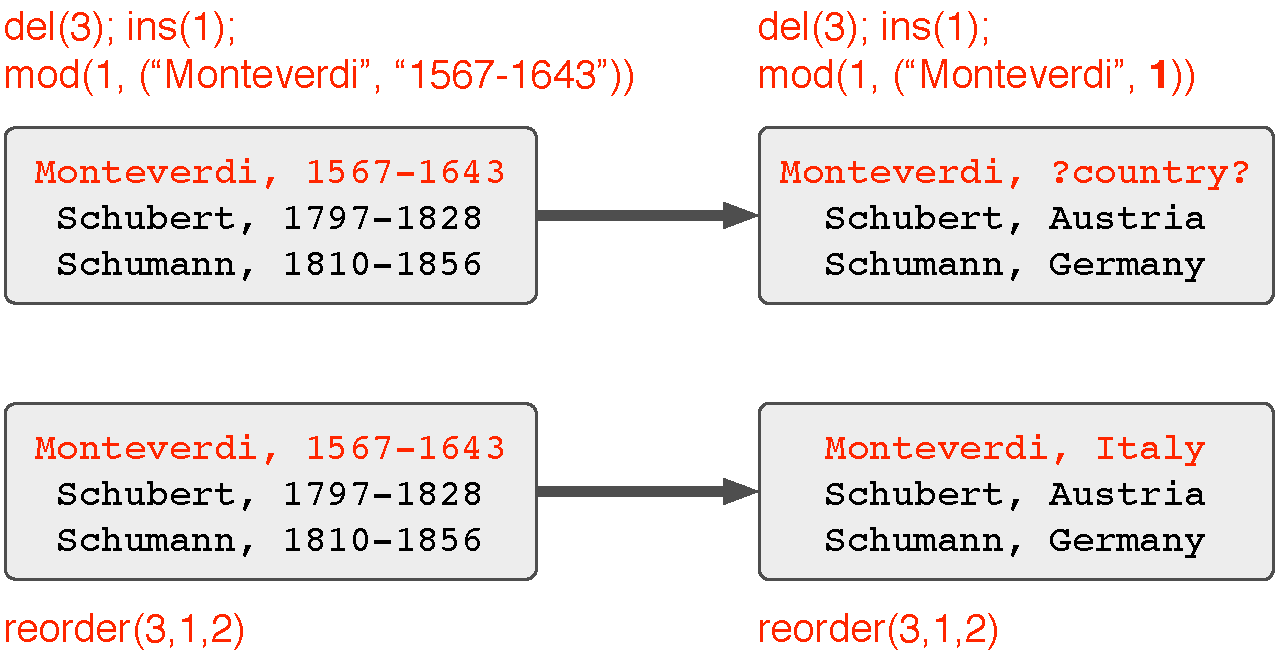
\includegraphics[width=75mm]{images/ex1-5.pdf} \\
        (f) two different edits with the same effect on the left
    \end{center}
\iflater
\discuss{Change the font everywhere to sf}
\fi
    \caption{A simple (complement-less) {\edit} lens in action.}
    \ifdissertation\draftspaced\fi
    \label{fig:example-simple}
\end{figure}

Before diving into technicalities, let's take a brief tour of the main
ideas via some examples.
%
Figure~\ref{fig:example-simple} demonstrates a simple use of {\edit} lenses
to synchronize two replicas\footnote{We use the word ``synchronize''
  informally to mean simply ``maintain a correspondence between two replicas
  by propagating edits in both directions.''  A full-blown synchronization
  tool would also include, at a minimum, some mechanism for dealing with
  conflicts between disconnected edits to the two structures, which is
  outside the scope of this paper.  \iffull Note, though, that we go beyond most
  synchronization tools in allowing the replicas to be structured
  differently and to share only a part of their information.\fi}.  In part (a),
we see the initial replicas, which are in a synchronized state.  On the
left, the replica is a list of records describing composers' birth and death
years; on the right,  a list of records describing the same
composers' countries of origin.  In part (b), the user interacting with the
left-hand replica decides to add a new composer, {\sf Monteverdi}, at the
end of the list.  This change is described by the edit script
{\sf
ins(3); mod(3, (``Monteverdi'', ``1567-1643''))}.
The script says to first
\emph{insert} a dummy record at index three, then \emph{modify} this record by
replacing the left field with ``{\sf Monteverdi}'' and replacing the 
right field with ``{\sf 1567-1643}''.  (One could of course imagine other edit
languages where the insertion would be done in one step.  We represent it
this way because this is closer to how our generic ``container mapping''
combinator in \S \ref{sec:containers} will do things.)  The
lens connecting the two replicas now converts this edit script into a
corresponding edit 
script that adds {\sf Monteverdi} to the right-hand replica, shown in part (c):
{\sf
ins(3); mod(3, (``Monteverdi'', \ONE))}.
Note that the translated {\sf mod} command overwrites the name component but
leaves the country component with its default value, ``{\sf
  ?country?}.''  This is the best it can do, since the edit was in
the left-hand replica, which doesn't mention countries.  
%
Later, an eagle-eyed editor notices the missing country information and
fills it in, at the same time correcting a spelling error in {\sf
  Schumann}'s name, as shown in (d). In part (e), we see that the lens
discards the country information when
translating the edit from right to left, but propagates the spelling
correction. 

Of course, a particular new replica state can potentially be
achieved by many different edits, and these edits may be translated differently.
%
Consider part (f) of Figure~\ref{fig:example-simple}, where the left-hand
replica ends up with a row for {\sf Monteverdi} at the beginning of the
list, instead of at the end. Two edit scripts that achieve this
effect are shown. The upper script deletes
the old {\sf Monteverdi} record and inserts a brand new one (which happens
to have 
the same data) at the top; the lower script rearranges the order of the
list.  The translation of the upper edit leaves {\sf Monteverdi} with a
default country, while the lower edit is translated to a
rearrangement, preserving all the information associated with {\sf
  Monteverdi}.% 

We do not address the question of where these edits come from or who
decides, in cases like part (f), which of several possible edits is
intended.  As argued in~\cite{Matching10}, answers to these questions will
tend to be intertwined with the specifics of particular editing and/or
diffing tools and will tend to be messy, heuristic, and
domain-specific---unpromising material for a foundational theory.  Rather,
our aim is to construct a theory that shows how edits, however
generated, can be translated between replicas of different shapes.

\iflater\finish{A lot of people got lost at this point.  We need to go much more
  gently.  (In particular, start with a roadmap.)  It would help to rename
  $X,Y,Z$ to something more mnemonic.}\fi

Abstractly, the lens we are discussing maps between structures of the form
$(X \times Y)\LIST$ and ones of the form $(X \times Z)\LIST$, where $X$ is the set
of composer names, $Y$ the set of date strings, and $Z$ the set of
countries.  We want to build it compositionally---that is, the whole lens
should have the form $\ell\LIST$, where $-\LIST$ is a ``list mapping'' lens
combinator and $\ell$ is a lens for translating edits to a
single record---i.e., $\ell$ is a lens from $X \times Y$ to $X \times Z$.
Moreover, $\ell$ itself should be built as the product $\ell_1 \times
\ell_2$ of a lens $\ell_1 \in X \to X$ that translates composer edits
verbatim, while $\ell_2$ is a ``disconnect'' lens that maps every edit on
either side to a trivial identity edit on the other side.

In analogous fashion, the edit languages for the top-level structures will
be constructed compositionally.  The set of edits for structures of the form
$(X \times Y)\LIST$, written $\partial ((X \times Y)\LIST)$, will be defined
together with the list constructor $-\LIST$.  Its elements will have the form
$\mlins{i}$ where $i$ is a position, $\mldel{i}$,
$\mlreorder{i_1,\ldots,i_n}$ where $i_1,\ldots,i_n$ is a permutation on
positions (compactly represented, e.g. as a branching program),
\iflater\discuss{people will be suspicious here---how do we know we
  can represent it compactly?}\fi and $\mlmod{p}{\dv}$, where $\dv \in
\partial (X\times Y)$ is an edit for $X \times Y$ structures.  Pair edits
$\dv \in \partial (X \times Y)$ have the form $\partial X \times
\partial Y$, where $\partial X$ is the set of edits to composers and
$\partial Y$ is the set of edits to dates.  Finally, both $\partial
X$ and $\partial Y$ are sets of primitive ``overwrite edits'' that completely
replace one string with another, together with an identity edit $\ONE$
that does nothing at all; so $\partial X$ can be just $\{\unit\} + X$ (with
$\ONE = \mlinl\unit$) and similarly for $Y$ and $Z$.

%% We write $\ONE$ instead of $\mlinl\ONE$ and {\sf
%%   ``x''} instead of $\mlinr x$ in contexts where it is clear that an edit of
%% this form is expected.

%% We can represent an edit to an element of $X \times Y$ as a pair of
%% edits to $X$ and $Y$; that is, $\partial(X \times Y) = \partial X \times
%% \partial Y$.  The application function $\odot_{X \times Y}$ simply applies
%% each of the component edits to the appropriate parts of the
%% product:
%% \iffull \[ \else $ \fi
%% (\dx,\dy) \odot_{X \times Y} (x, y) = (\dx \odot_X x, \dy \odot_Y y)
%% \iffull .\] \else $. \fi
%% We sometimes write $\mlonl\dx$ as an alias for $(\dx,\ONE)$ when we want to
%% emphasize that a particular edit affects only one part of a tuple, and
%% similarly for $\mlonr\dy$.

Our lens $\ell\LIST$ will consist of two components---one for transporting edits
from the left side to the right, written $(\ell\LIST).\dputr \in \partial(X
\times Y)\LIST \to \partial(X \times Z)\LIST$,\footnote{The symbol $\dputr$ is
  pronounced ``put an edit through the lens from left to right,'' or just
  ``put right.''  It is the {\edit}-analog of the $\putr$ function of the
  state-based symmetric lenses in\symmlenses and the
  $\PUT$ function of the state-based asymmetric lenses
  in~\cite{Focal2005,Boomerang07}.} and another for transporting
edits from right to left, written $(\ell\LIST).\dputl \in \partial(X \times
Z)\LIST \to \partial(X \times Y)\LIST$.
%

%% The next step is to lift this translation to lists.  There are two kinds of
%% edits to lists in the example\finish{why is it this way?}:
%% \emph{rearrangements}, which modify the 
%% structure of the list via insertions of dummy elements, deletions, 
%% reorderings (but which do not modify the elements themselves), and
%% \emph{modifications} of the values in the list using the underlying element
%% edits (which do not affect the list structure or order).  We already know
%% how to translate modifications, and rearrangements are easy because the list
%% structure is the same on both sides.  Putting these observations together
%% gives us a translation function $\ell^*.\dputr \in \partial((X\times Y)^*)
%% \to \partial((X \times Z)^*)$ for list edits (the $\dputl$ function is
%% similar): 
%% \iffull
%%   \begin{align*}
%%     \ell^*.\dputr(\mlins i) &= \mlins i \\
%%     \ell^*.\dputr(\mldel i) &= \mldel i \\
%%     \ell^*.\dputr(\mlreorder{i_0,\ldots,i_n}) &= \mlreorder{i_0,\ldots,i_n} \\
%%     \ell^*.\dputr(\mlmod ie) &= \mlmod i{\ell.\dputr(e)}
%%   \end{align*}
%% \else
%% \[
%% \begin{array}{lcl}
%%     \ell^*.\dputr(\di) &=& \di \\&& \mbox{if $\di$ is an $\mlins$,
%%     $\mldel$, or $\mlreorder$}\\
%%     \ell^*.\dputr(\mlmod ie) &=& \mlmod i{\ell.\dputr(e)}
%% \end{array}
%% \]
%% \fi
%% \iflater
%% \bcp{Not exactly sure what we want to say about this---cutting from the
%%   short version.}
%% The reader may wonder why we break list insertions into
%% two stages---first inserting a dummy element and then modifying this dummy
%% element with desired data. The ease of writing the above function is 
%% the answer: since the former stage does not mention elements of the list at
%% all, we need not do any translation, and since the latter stage is
%% simply an edit script, we may dispatch to the underlying lens. 
%% \fi
%% %% Additionally,
%% %% the breakdown lets us preserve a nice factorization property that we discuss
%% %% in the next section.\bcp{where? refer to it by number?}

\begin{figure}
    \ifdissertation\newcommand\lw{0.9\linewidth}\else\newcommand\lw\linewidth\fi
    \begin{tabular}{c}
        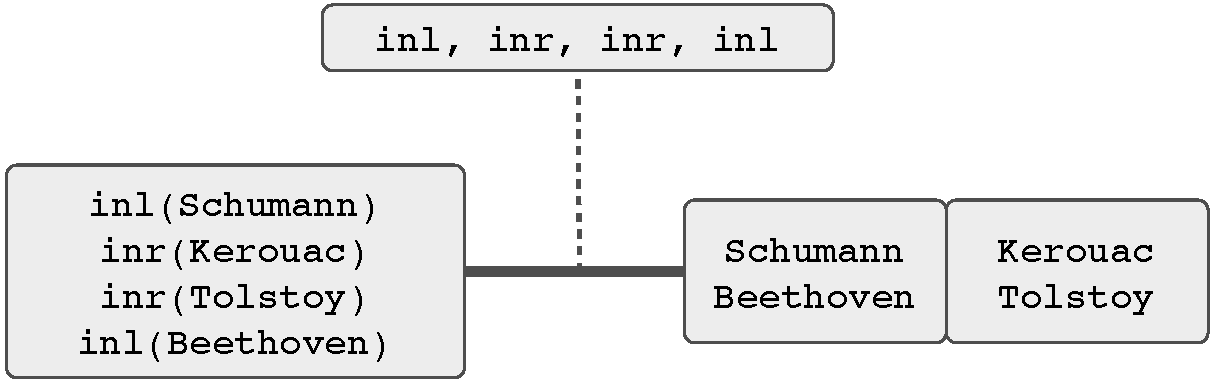
\includegraphics[width=75mm]{images/ex2-0.pdf} \\[.9ex]
        \parbox \lw{(a) the initial replicas: a tagged list of composers and authors on
        the left; a pair of lists on the right; a complement storing just
        the tags}
        \\[3ex]
        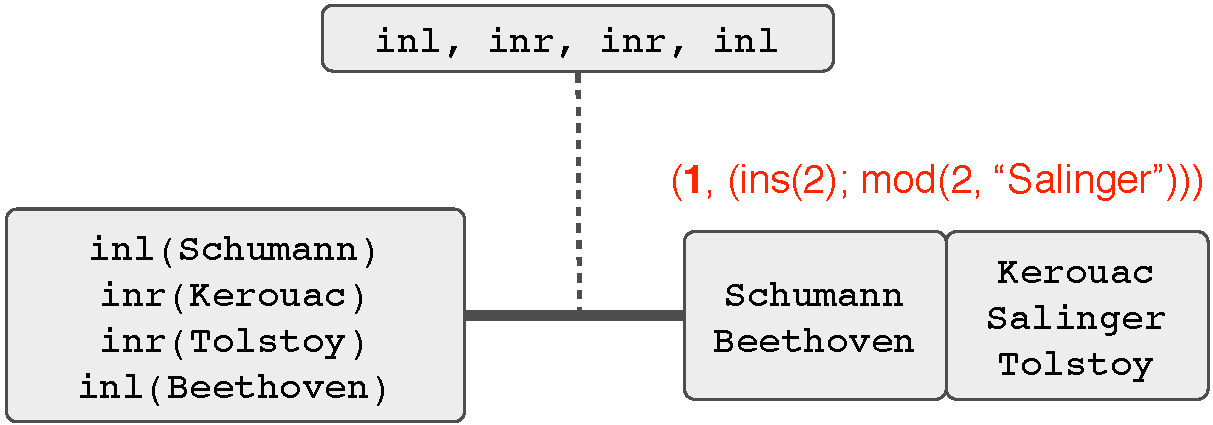
\includegraphics[width=75mm]{images/ex2-1.pdf} \\
        \parbox \lw{\begin{center}(b) an element is added to one of
            the partitions\end{center}} \\[2ex]
        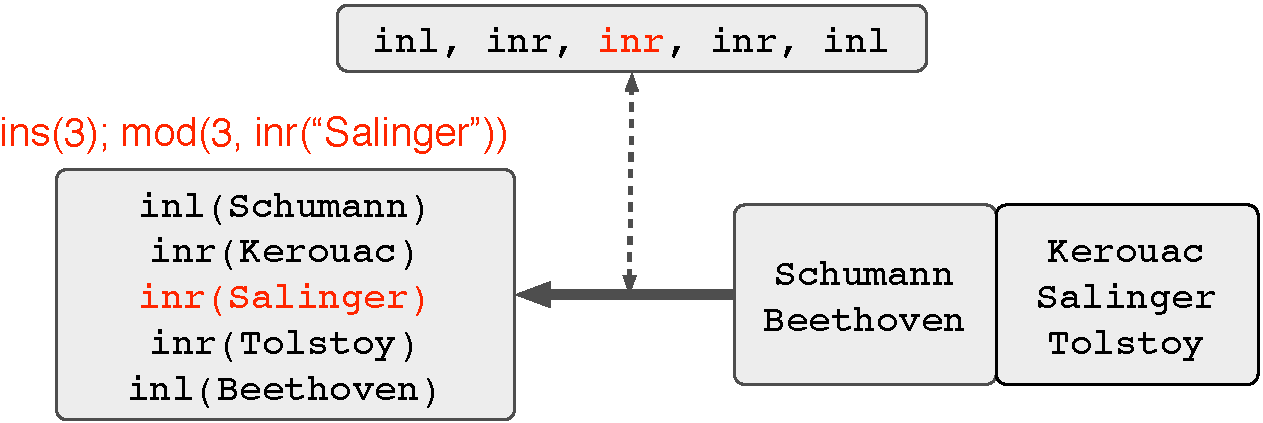
\includegraphics[width=75mm]{images/ex2-2.pdf} \\
        \parbox \lw{\begin{center}(c) the complement tells how to translate the
            index\end{center}} \\[.7ex]
    \end{tabular}
    \caption{A lens with complement.}
    \label{fig:example-partition}
\end{figure}

We sometimes need lenses to have a little more structure than this simple
example suggests. 
To see why, consider defining a {\em partitioning} lens $p$ between
the sets $\partial((X+Y)\LIST)$ and $\partial(X\LIST \times Y\LIST)$.
Figure~\ref{fig:example-partition} demonstrates the behavior of this lens.
%
In part (a), we show the original replicas: on the left, a single list that
intermingles authors and composers (with {\sf inl/inr} tags showing which is
which), and on the right a pair of homogeneous (untagged) lists, one for
authors and one for composers. Now consider an edit, as in (b), that inserts
a new element somewhere in the author list on the right. It is clear that we
should transport this into an insertion on the left replica, but where, exactly,
should we insert it?  If the $\dputl$ function is given just an
insertion edit for the homogeneous author list and nothing else, there is no
way it can translate this edit into a sensible position in the combined list
on the left, since it doesn't know how the lists of authors and composers
are interleaved on the left.  

\iflater\bcp{People were not clear on why the complement was needed.  Also, in this
  example, even with the complement, there is still some arbitrary choice in
  where an inserted element on the right appears in the list on the left.}\fi

The solution is to store a small list, called a {\em complement}, off to the
side, recording the \emph{tags} ($\ml{inl}$ or $\ml{inr}$) from the
original, intermingled list, and pass this list as an extra argument to
translation.  We then enrich the types of the edit translation functions to
accept a complement and return a new complement, so that
%
\iffull \[ \else $ \fi
p.\dputr \in \partial((X+Y)\LIST) \times C \to \partial(X\LIST \times Y\LIST)
\times C
\iffull \] \else $ \fi
and
\iffull \[ \else $ \fi
p.\dputl \in \partial(X\LIST \times Y\LIST) \times C \to \partial((X+Y)\LIST)
\times C
\iffull .\] \else $. \fi
Part (c)
demonstrates the use (and update) of the complement when translating the
insertion.

Note that the complement stores just the {\sf inl/inr} tags, not the actual
names of the authors and composers in the left-hand list.  \iflater\finish{This next
statement made people suspicious---we need to go into more detail.}\fi In general, the
information stored in $C$ will be much smaller than the
information in the replicas; indeed, our earlier example illustrates the
common
case in which $C$ is the trivial single-element set $\Unit$.  The
translation functions manipulate just the complements and the edits, which
are also small compared to the size of the replicas.

%% \finish{Someplace, we need to talk about what happens to edits that don't
%%   make sense on the current state.  There are three possibilities, with a
%%   tradeoff between size of representations and ``accuracy'' of edits:
%%   \begin{itemize}
%%   \item Embed a description of the exact state in the edit and say that the
%%   edit only applies to this state.  This is what Diskin, etc., do.  But it
%%   means that edits are very large.
%%   \item Allow any edit to apply to any state.  Then there are two
%%   sub-possibilities:
%%   \begin{itemize}
%%   \item keep it total but make it behave like the identity (or some other
%%   arbitrary choice) anywhere it doesn't ``make sense''
%%   \item make it partial
%%   \end{itemize}
%%   \end{itemize}
%% }
%% \finish{
%% Old text: Other authors model {\edit}s in other ways; for example, Stevens
%% \finish{citation} chooses functions whose domain and range are equal.
%% Functions are a nice model in some circumstances, but are difficult to
%% inspect: the only operation that can be performed is to apply them to some
%% concrete argument.  Monoids subsume these functions, and some instantiations
%% offer more reflective representations of edits.}

\sect{Edit Lenses}
\label{sec:semantics}

A key design decision in our formulation of edit lenses is to separate the
{\em description} of edits from the {\em action} of applying an edit to a
state.  This separation is captured by the standard mathematical notions of
{\em monoid} and {\em monoid action}.

\begin{defn}
%% \bcp{why do we say a triple here and in
%%     3.2.3, but other places just name the components (e.g., defn of
%%     category)?} 
A \emph{monoid} is a triple $\left<M,\cdot_M,\ONE_M\right>$ of a set
$M$, an associative binary operation $\cdot_M \in M \times M
\to M$, and a unit element $\ONE_M \in M$ --- that is, with $\cdot_M$ and $\ONE_M$ such that
\iffull
\begin{eqnarray*}
x\cdot_M(y\cdot_M z) = (x\cdot_M y) \cdot_M z\\
\ONE_M\cdot_M x = x = x \cdot_M \ONE_M .
\end{eqnarray*}
\else
$x\cdot_M(y\cdot_M z) = (x\cdot_M y) \cdot_M z $ and
$\ONE_M\cdot_M x = x = x \cdot_M \ONE_M$.
\fi
\end{defn}
When no confusion results, we use $M$ to denote both the set and the
monoid, drop subscripts from $\cdot$ and $\ONE$, and write $mn$ for
$m \cdot n$.  
%% In more standard terminology, a ``monoid'' in our sense would
%% be called a \emph{partial monoid}\iflater~\cite{partialmonoids}\fi, but
%% since we always work with partial monoids we find it convenient to drop the
%% qualifier.

The unit element represents a ``change nothing'' edit.  Multiplication of
edits corresponds to packaging up multiple edits into a single one
representing their combined effects\iffull{} (this might be useful, for example, for
offline editing)\fi.

Modeling edits as monoid elements gives us great flexibility in 
concrete representations.
%
The simplest edit language is a {free monoid} whose elements are just words
over some set of primitive edits and whose multiplication is
concatenation.  
%
However, it may be useful to put 
more structure on edits, either (a) to allow 
more compact representations or (b) to capture the intuition that edits to
different parts of a structure do not interfere with each other and can thus
be applied in any order.  We will see an example of (b) in 
\S \ref{sec:monoid-laws}. For a simple example of 
(a), recall from
\S \ref{sec:delta-examples} that, for every set $X$, we can form an {\em
  overwrite} monoid where the edits are just the elements of $X$ together
with a fresh unit element---i.e., edits can be represented as elements of
the disjoint union $\Unit + X$. Combining two edits in this monoid
simply drops the second (unless the first is the unit):
\iffull
\[
\mlinl{\unit} \cdot e = e \qquad
\mlinr{x} \cdot e = \mlinr x
\]
\else
$\mlinl{\unit} \cdot e = e$ and $\mlinr{x} \cdot e = \mlinr x$.
\fi
These equations allow this edit language to represent an arbitrarily long
sequence of updates using a single element of $X$ (and, {\em en passant}, to
recover state-based lenses as a special case of edit lenses). \iflater\bcp{Would it
  actually work to build a whole set of lens combinators with these edits?
  Or are we just saying that, for an arbitrary set $X$, there is an identity
  lens on this module over $X$?  What, exactly, are we saying?}\fi
%
The monoid framework can also accommodate more abstract notions of edit.  For
example, the set of all total functions from a set $X$ to itself forms a
monoid, where the multiplication operation is function composition.  This is
essentially the form of edits considered by
Stevens~\cite{stevens2008tat}\iflater\finish{Not just Stevens---we should
  find a few more citations for this idea.}\fi.  \iflater\bcp{Same question for this one.  At a minimum, we should say that we are not dealing with these examples in detail in the rest of the paper.}\fi
%
We mostly focus on the simple case where edit languages are free monoids.
\S \ref{sec:monoid-laws} considers how additional laws can be added to the
product and sum lens constructions\iffull (laws for lists and general
containers are left for future work)\fi.

\begin{defn}
    Given a  monoid $M$ and a set $X$, a \emph{monoid action} on $M$ and $X$
    is a partial function $\odot \in M \times X \partialto X$ satisfying two laws:
\iffull
    \infax{\ONE \odot x = x}
    \infax{(m \cdot n) \odot x = m \odot (n \odot x)}
\else
$\ONE \odot x = x$ and $(m \cdot n) \odot x = m \odot (n \odot x)$.
\fi
\end{defn}
%
As with monoid multiplication, we often elide the monoid action symbol,
writing $mx$ for $m \odot x$.  In standard mathematical terminology, a
monoid action in our sense might instead be called a ``partial monoid
action,'' but since we always work with partial actions we find it
convenient to drop the qualifier.

A bit of discussion of partiality is in order.  
Multiplication of edits is a total operation: given two descriptions of
edits, we can always find a description of the composite actions of doing
both in sequence.  On the other hand, {\em applying} an edit to a particular
state may sometimes fail.
%
This means we need to work with expressions and equations involving
partial operations. As usual, any term that contains an undefined
application of an operation to operands is undefined---there is no way of
``catching'' undefinedness. An equation between possibly undefined terms 
(e.g., as in the definition above) 
means that if either side is defined then so is the other, and their values
are equal (Kleene equality).

Why deal with failure explicitly, rather than keeping edit application total
and simply defining our monoid actions so that applying an edit in a state
where it is not appropriate yields the same state again (or perhaps some
other state)?  One reason is that it seems natural to directly address the
fact that some edits are not applicable in some states, and to have a
canonical outcome in all such cases.  A more technical reason is that, when
we work with monoids with nontrivial equations, making inapplicable edits
behave like the identity is actually
wrong.%
%
\footnote{Here is a slightly contrived example.  Suppose that the set of
  states is natural numbers and that edits have the form $(x\mapsto y)$,
  where the intended interpretation is that, if the current state is $x$,
  then the edit yields state $y$.  It is reasonable to impose the equation
  $(y\mapsto z)\cdot(x\mapsto y) = (x\mapsto z)$, allowing us to represent
  sequences of edits in a compact form.  But now consider what happens when
  we apply the edit $(5\mapsto 7)\cdot(3\mapsto 5)$ to the state $5$.  The
  second monoid action law demands that $((5\mapsto 7)\cdot(3\mapsto 5))
  \odot 5 = (5\mapsto 7)\odot((3\mapsto 5) \odot 5)$, which, by the equation
  we imposed, is the same as $(3\mapsto 7) \odot 5 = (5\mapsto
  7)\odot((3\mapsto 5) \odot 5)$.  But the left-hand side is equal to $5$
  (since the edit $(3\mapsto 7)$ does not apply to the state $5$), while the
  right-hand side is equal to $7$ (since the first edit, $(3\mapsto 5)$, is
  inapplicable to the state $5$, so it behaves like the identity and returns
  $5$ from which $(5\mapsto 7)$ takes us to $7$), so the action law is
  violated.}

However, although the framework allows for the possibility of edits failing,
we still want to know that the edits produced by our lenses will never
actually fail when applied to replica states arising in practice.  This
requirement, corresponding to the {\em totality} property of previous
presentations of lenses~\cite{Focal2005}, is formalized in Theorem
\ref{nofail}.  In general, we adopt the design principle that partiality
should be kept to a minimum; this simplifies the definitions.

%% Notice that the second law implies that if $m\odot(n\odot x)$ is
%% defined then $m\cdot n$ must be defined and conversely, if $n\odot x$
%% is undefined then $(m\cdot n)\odot x$ must also be undefined for all
%% $m$ even if $m\cdot n$ is defined.

\iflater
\finish{A monoid action is a monoid homomorphism from $M$ to $X \to X$. Can
tie this back to the Stevens work, too, maybe?}
\fi

It is convenient to bundle a particular choice of monoid and monoid
action, plus an initial element, into a single structure:

\begin{defn}
    A \emph{module} is a tuple $\left<X,\, \init_X,\, \partial
    X,\,\odot_X\right>$ comprising a set $X$, an element $\init_X\in X$, a monoid 
    $\partial X$, and a monoid action $\odot_X$ of $\partial X$ on $X$.
\end{defn}
If $X$ is a module, we refer to its first component by either
$|X|$ or just $X$, and to its last component by $\odot$ or simple
juxtaposition.

We will use modules to represent the structures connected by lenses.  Before
coming to the definition of lenses, however, we need one last ingredient:
the notion of a {\em stateful homomorphism} between monoids.  As we saw in
\S \ref{sec:delta-examples}, there are situations where the information in an
edit may be insufficient to determine how it should be translated---we may
need to know something more about how the two structures correspond. The
exact nature of the extra information needed varies according to the lens.
%
To give lenses a place to store such auxiliary information, we
follow\symmlenses and allow the edit-transforming
components of a lens (the $\dputr$ and $\dputl$ functions) to take a {\em
  complement} as an extra input and return an updated complement as an extra
output.
%
\iflater
\discuss{Not sure there's time to change it now, but I found while writing
  that explanation that the word ``complement'' was quite awkward---I kept
  wanting to say just ``state.''  Moreover, the term is technically a bit
  tenuous now, since what we store is not, in fact, anything like a
  complement in the old database sense.}  \soon{complement becomes correspondence}
\fi

\begin{defn}
Given monoids $M$ and $N$ and a {\em complement set} $C$, a \emph{stateful monoid
  homomorphism} from $M$ to $N$ over $C$ is a function $h \in M \times C \to
N \times C$ satisfying two laws:
%
\vspace*{-1ex}
\infrule{}{h(\ONE_M,c) = (\ONE_N,c)}
\infrule{
         h(m,c) = (n,c') \andalso h(m',c') = (n',c'')
}{
         h(m' \cdot_M m,c) = (n' \cdot_N n,c'')
}
%
These are basically just the standard monoid homomorphism laws, except that
$h$ is given access to some internal state $c \in C$ that it uses (and
updates) when mapping from $M$ to $N$; in the second law, we must thread the
state $c'$ produced by the first $h$ into the second use of $h$, and we
demand that both the result and the effect on the state should be the same
whether we send a composite element $m' \cdot m$ through $h$ all at once or
in two pieces.
\end{defn}

The intended usage of an edit lens is as follows. There are two users,
one holding an element of $X$ the other one an element of $Y$, both
referred to hereafter as {\em replicas}.  Initially, they hold $\init_X$ and
$\init_Y$, respectively, and the lens is initialized with complement
$\ell.\missing$. The users then perform actions and propagate them across
the lens. An action consists of producing an edit $\dx$ (or $\dy$), applying
it to one's current replica $x$ (resp.\ $y$), putting the edit through the lens
to obtain an edit $\dy$ (resp.\ $\dx$), and asking the user on the other
side to apply $\dy$ ($\dx$) to their replica.  In the process, the internal
state $c$ of the lens is updated to reflect the new correspondence between
the two replicas.
\iffull

\fi%
We further assume there is some {\em consistency} relation $K$ between $X$,
$Y$, and $C$, which describes the ``synchronized states'' of the replicas
and complement.  This gives us a natural way to state the totality
requirement discussed above: if we start in a consistent state, make a
successful edit (one that does not fail at the initiating side), and put it
through the lens, the resulting edit is guaranteed (a) to be applicable on
the receiving side and (b) to lead again to a consistent state.  We make no
guarantees about edits that fail at the initiating side: these should not be
put through the lens.

\begin{defn}\label{defn:lens}
A \emph{symmetric edit lens} between modules $X$ and $Y$ consists of a
complement set $C$, a distinguished element $\missing\in C$, 
two stateful monoid homomorphisms 
\iffull
\[
\begin{array}{lcl}
\dputr &\in& \partial X \times C \to \partial Y \times C \\
\dputl &\in& \partial Y \times C \to \partial X \times C
\end{array}
\]
\else
$\dputr \in \partial X \times C \to \partial Y \times C$ and
$\dputl \in \partial Y \times C \to \partial X \times C$, 
\fi
%
%% total functions 
%% \[
%% \begin{array}{lcl}
%% \dputr &\in& \partial X \times C \to \partial Y \times C \\
%% \dputl &\in& \partial Y \times C \to \partial X \times C
%% \end{array}
%% \]
%% such that \infax{\dputr(\ONE,c)=(\ONE,c) \qquad \dputl(\ONE,c)=(\ONE,c)}
%% \infrule{ \dputr(\dx_2,c)=(\dy_2,c') \quad
%%   \dputr(\dx_1,c')=(\dy_1,c'') }{ \dputr(\dx_1\ \dx_2,c)=(\dy_1\
%%   \dy_2, c'') } \infrule{ \dputl(\dy_2,c)=(\dx_2,c') \quad
%%   \dputl(\dy_1,c')=(\dx_1,c'') }{ \dputl(\dy_1\ \dy_2,c)=(\dx_1\
%%   \dx_2, c'') } 
and a ternary {\em consistency relation}
$K\subseteq |X|\times C\times |Y|$ such that
\begin{itemize}
\item $(\init_X,\missing,\init_Y)\in K$;
\item if $(x,c,y)\in K$ and $\dx\ x$ is defined and $\dputr(\dx,c)=(\dy,c')$, then $\dy\ y$ is also defined and $(\dx\ x,c',\dy\ y)\in K$;
\item if $(x,c,y)\in K$ and $\dy\ y$ is defined and $\dputl(\dy,c)=(\dx,c')$, then $\dx\ x$ is also defined and $(\dx\ x,c',\dy\ y)\in K$.%
%
\iffull
\footnote{One might consider a more general format with ``creation''
  operations $\creater\in X\rightarrow Y\times C$ and symmetrically
  $\createl$.  This format actually arises as a special case of the one
  above by choosing the edit monoids to include operations of the form
  $\text{set}(x)$ for $x\in X$, with action $\text{set}(x)\odot x'=x$. One
  can then define $\creater(x,c) = \dputr(\text{set}(x),c)$.}
\fi
%
\end{itemize}
% \discuss{BCP will add a note about binary consistency relations.  Dual role: Important sanity check on dputs, but also a part of the external specification of the lens.}
\end{defn}
Since symmetric edit lenses are the main topic of this paper, we will
generally write ``edit lens'' or just ``lens'' for these,
deploying additional adjectives to talk about other variants such
as \iflater\finish{the asymmetric variant or} \fi the state-based
symmetric lenses of\symmlenses.

The intuition about $K$'s role in guaranteeing totality can be formalized as
follows.

\begin{defn}
Let $\ell \in X\lens Y$ be a lens. A \emph{dialogue} is a sequence of
edits---a word in $(\partial X+\partial Y)\LIST$. The {partial}
function
\iffull\[\else $ \fi
\ell.\run \in (\partial X+\partial Y)\LIST\partialto   X\times   \ell.C\times Y
\iffull\]\else $ \fi
is defined by:
\infrule{}{\ell.\run(\NIL) = (\init_X,\ell.\missing,\init_Y)}
\infrule{
    \ell.\run(w)=(x_0,c,y_0)
    \andalso  
    \ell.\dputr(\dx_1,c)=(\dy_1,c_1)
  }{
    \ell.\run(\mlinl{\dx_1} \CONS w) = (\dx_1\,x_0,c_1,\dy_1\,y_0)
  }
\infrule{
    \ell.\run(w)=(x_0,c,y_0)
    \andalso  
    \ell.\dputl(\dy_1,c)=(\dx_1,c_1)
  }{
    \ell.\run(\mlinr{\dy_1} \CONS w) = (\dx_1\,x_0,c_1,\dy_1\,y_0)
  }
\end{defn}

\begin{theorem}\label{nofail}
Let $w$ be a dialogue and suppose that $\ell.\run(w)=(x,c,y)$---in
particular, all the edits in $w$ succeed.
Let $\dx\in\partial X$ be an edit with $\dx\ x$ defined. If
$(\dy,c')=\ell.\dputr(\dx,c)$ then $\dy\ y$ is also defined. An analogous
statement holds for $\dputl$.
\end{theorem}

\iffull
\begin{proof}
By induction on $w$ we can easily show that $(x,c,y)\in \ell.K$. The claim
then follows from the axioms for lenses.
\end{proof}
\fi

\iflater \finish{We need some discussion of why these laws are the
  right ones.  One justification is that they are essentially just
  (stateful versions of) the monoid homomorphism laws.  Another is
  that they give rise to a nice correspondence with state-based lenses
  (is that true?).}  \fi

Beyond its role in guaranteeing totality, the consistency relation in a lens
plays two important roles.  First, it is a sanity check on the behavior of
$\dputr$ and $\dputl$.  Second, if we project away the middle component, we
can present it to programmers as documentation of the synchronized states of
the two replicas---i.e., as a partial {\em specification} of $\dputr$ and
$\dputl$.

One technical issue arising from the definition of edit lenses is that the
hidden complements cause many important laws---like associativity of
composition---to hold only up to {\em behavioral equivalence}.  This phenomenon
was also observed in \ifdissertation\S\ref{equiv}\else\cite[\S
3]{HofmannPierceWagner10}\fi\ for the case of
symmetric state-based lenses, and the appropriate behavioral equivalence
for edit lenses is a natural refinement of the one used there (taking the
consistency relations into account).

\begin{defn}[Lens equivalence]
Two lenses $k,\ell:X\lens Y$ are {\em equivalent} (written $k \equiv \ell$) if,
for all dialogues $w$, 
\begin{itemize}
\item $k.\run(w)$ is defined iff $\ell.\run(w)$ is defined;
\item if $k.\run(w)=(x,c,y)$ and $\ell.\run(w)=(x',d,y')$, then $x=x'$ and
$y=y'$; and
\item if  $k.\run(w)=(x,c,y)$ and $\ell.\run(w)=(x',d,y')$ and $\dx\ x$ is defined and $\ell.\dputr(\dx,c)=(\dy,\_)$ and 
 $k.\dputr(\dx,d)=(\dy',\_)$ then $\dy=\dy'$, and the analogous property for $\dputl$. 
\end{itemize} 
\end{defn}
(Note that the second clause is actually implied by the third.)
% We write $X \Lens Y$ for the set of equivalence classes of lenses
% from $X$ to $Y$.  When $\ell$ is a lens, we write $\EQCLASS{\ell}$
% for the equivalence class of $\ell$ (that is, $\ell \in X\lens Y$
% iff $\EQCLASS{\ell} \in X\Lens Y$).  Where no confusion results, we
% abuse notation and drop these brackets, using $\ell$ for both a lens
% and its equivalence class.  \finish{Do we actually need this
%   convention now?  Doesn't seem like we're making much use of
%   equivalence classes in this paper.}
% \end{defn}

Since the complements of the two lenses in question may not even have
the same type, it does not make sense to require that they be
equal. Instead, the equivalence hides the complements, relying on the
observable effects of the lens actions. However, by finding a
relationship between the complements, we can prove lens
equivalence with a bisimulation-style proof principle:
\begin{theorem}\label{thm:bisim}
Lenses $k,\ell:X\lens Y$ are equivalent iff there exists a relation
$S\subseteq X\times k.C\times \ell.C\times Y$ such that  
\iffull \begin{itemize} \fi
\iffull \item \else (1) \fi $(\init_X,k.\missing,\ell.\missing,\init_Y)\in S$;
\iffull \item \else (2) \fi if $(x,c,d,y)\in S$ and $\dx\ x$ is defined, then if $(\dy_1,c')=
k.\dputr(\dx,c)$ and $(\dy_2,d')=
\ell.\dputr(\dx,d)$, then $\dy_1=\dy_2$ and $(\dx\ x,c',d',\dy_1\ y)\in
S$; and
\iffull \item \else (3) \fi analogously for $\dputl$. 
\iffull \end{itemize} \fi
\end{theorem}

\iffull
\begin{pf}
  For the ``if'' direction we prove by induction on dialogues that if
  $k.\run(w)$ is defined then so is $\ell.\run(w)$ and vice versa and
  if $k.\run(w)=(x,c,y)$ and $\ell.\run(w)=(x',d,y')$ then $x=x'$ and
  $y=y'$ and $(x,c,d,y)\in S$. For the converse we define
  $(x,c,d,y)\in S$ iff there exists a dialogue $w$ such that
  $k.\run(w)=(x,c,y)$ and $\ell.\run(w)=(x,d,y)$ 
% \finish{Checked that
%     this proof is good for the new notion of equivalence. }
\end{pf}

\begin{theorem}
    Lens equivalence is an equivalence relation.
\end{theorem}
\begin{pf}
    Reflexivity: the set $\{(x,c,c,y) \mid (x,c,y) \in \ell.K\}$ witnesses the
    equivalence $\ell\equiv\ell$ for any $\ell$.

    Symmetry: if the set $S$ witnesses the equivalence $k\equiv\ell$, then
    the set $\{(x,d,c,y) \mid (x,c,d,y) \in S\}$ witnesses the equivalence
    $\ell \equiv k$.

    Transitivity: if $S$ witnesses $j \equiv k$ and $T$ witnesses
    $k\equiv\ell$, then
    \[\{(x,c,e,y) \mid \exists d. (x,c,d,y) \in S \land (x,d,e,y) \in T\}\]
    witnesses $j\equiv\ell$. The verification is straightforward.
\end{pf}
\fi

\iffull
\iflater
\discuss{Not sure exactly where this lemma belongs.  When is it used?}The
following lemma asserts that dialogues and runs make sense on the level of
equivalence classes. The proof is a direct induction on runs.
\begin{lemma}
Let $k,\ell \in X\lens Y$ be equivalent lenses ($k\equiv \ell$). Let $w$
be a dialogue and $k.\run(w)=(x,c,y)$ and
$\ell.\run(w)=(x',c',y')$. Then $x=x'$ and $y=y'$. 
\end{lemma}

\discuss{I find this next observation about not being visible at the level
  of equivalence classes to be more confusing than enlightening.  Could we
  just drop it?}
\discuss{Re-reading it, I tend to agree. Probably, we should rather dwell on 
the ``projecting out the complement'' point of view. --Martin}
The consistency relations $K$ are not visible at the level
of equivalence classes of lenses not least because they involve the
complement. As we have seen, their mere presence guarantees that reasonable
edits succeed and this phenomenon is observable at the level of equivalence
classes. But consistency relations are also useful to assert certain shared
properties between the states that are ``synchronized'' by the lens. We now
give a complement-free version of this:

\begin{defn}
A lens $\ell \in X\lens Y$ {\em maintains} a relation $R\subseteq X\times Y$ if,
for any dialogue $w$ and $\ell.\run(w)=(x,c,y)$, we have $x\mathrel{R}y$. 
\end{defn}

\begin{theorem}
If $k\equiv\ell$ are equivalent lenses between $X$ and $Y$, then $k$
maintains a relation $R$ iff $\ell$ does.
%
Moreover, $\ell$ preserves $R$ iff there exists a relation $S\subseteq
X\times\ell.C\times Y$ such that 
\begin{itemize}
\item $(\init_X,\ell.\missing,\init_Y)\in S$;
\item whenever $(x,c,y)\in S$ and
$\dx\ x$ is defined, $\dy\ y$ is also defined and $(\dx\ x,c',\dy\
y)\in S$ when $(\dy,c')=\dputr(\dx,c)$; 
\item the analogous condition for $\dputl$; and
\item $(x,c,y)\in S$ implies $(x,y)\in R$.
\end{itemize}
\end{theorem}

\iffull
\begin{pf}
The ``if'' direction is an easy induction on dialogues. For the ``only
if'' direction we use the relation $S=\{(x,c,y)\mid xRy\wedge \exists
w.\ell.\run(w)=(x,c,y)\}$. 
\finish{Needs to be updated for the new defn of equivalence.}
\end{pf}
\fi
\fi
\fi

\sect{Edit Lens Combinators}\label{sec:combinators}

\iflater\discuss{We don't actually formalize the ``overwrite edits'' lens
  constructor (which takes a set to a module).  We should, since we use it
  in Section 2!}\fi

\iflater
\finish{The extra (fibrationish) laws need to be checked for everything
  here.}\bcp{I guess we've dropped these laws now, but it would be nice to
  get back to discussing them someplace.}
\fi

We have proposed a semantic space of edit lenses and justified its design.
But the proof of the pudding is in the syntax---in whether we can actually
build primitive lenses and lens combinators that live in this semantic space
and that do useful things.

\paragraph*{Generic Constructions}

As a first baby step, here is an identity lens that connects identical
structures and maps edits by passing them through unchanged.

\iffull \begin{defn}[Identity]\  \fi
        \lensdef{w_id}
        {\id_X \in X \lens X}
        {
            C &=& \Unit \\
            K &=& \{ (x,\unit,x) \;|\; x \in X \} \\
            \dputr(\dx,\unit) &=& (\dx,\unit) \\
            \dputl(\dx,\unit) &=& (\dx,\unit)
}
%
Here and below, we elide the definition of the $\missing$ component when
$C=\Unit=\{\unit\}$, since it can only be one thing.

\iffull
\begin{lemma}\ 
    $\id.\dputr$ and $\id.\dputl$ are stateful homomorphisms, and the
    relation $\id.K$ is preserved.
    \label{id-goodlens}
\end{lemma}
\begin{proof}
    Showing that $\dputr$ is a homomorphism involves showing that
    $\id.\dputr(\ONE,\unit)=(\ONE,\unit)$, which is direct, and that if
    $\id.\dputr(\dx,c)=(\dy,c')$ and $\id.\dputr(\dx',c')=(\dy',c'')$,
    then $\id.\dputr(\dx'\dx,c)=(\dy'\dy,c'')$. Since $c=c'=c''=\unit$, it
    follows directly that $\dy=\dx$ and $\dy'=\dx'$, so the final claim is
    true. A similar argument shows that $\dputl$ is a homomorphism.

    To show that $K$ is preserved, choose a consistent triple
    $(x,\unit,x)$ and observe that $\dputr(\dx,\unit)=(\dx,\unit)$ results
    in another consistent triple $(\dx\;x,\unit,\dx\;x)$. A similar argument
    for $\dputl$ applies.
\end{proof}
\else
In lens definitions like this one, the upper box serves both as a typing
rule and as the implicit statement of a theorem saying that the functions in
the box below it inhabit the appropriate types and satisfy the corresponding lens
laws. For lens combinators, the definition also makes an implicit statement
about compatibility with lens equivalence. For brevity, and because they are
generally straightforward, we usually elide these theorems.
\fi
\iffull \end{defn} \fi

Now for a more interesting case:  Given lenses $k$ and $\ell$ connecting $X$ to
$Y$ and $Y$ to $Z$, we can build a composite lens $k;\ell$ that connects $X$
directly to $Z$.  Note how the complement of the composite lens includes
a complement from each of the components, and how these complements
are threaded through the $\dputr$ and $\dputl$ operations.
\iffull \begin{defn}[Composition]\  \fi
        \lensdef{w_composition}
        {\infruleplain{k \in X \lens Y \qquad \ell \in Y \lens Z}{k;\ell \in X \lens Z}}
        {
            C &=& k.C \times \ell.C \\
            \missing &=& (k.\missing , \ell.\missing) \\
            K &=& \{ (x,(c_k,c_\ell),z) \;|\; \\
                        && \qquad \exists y. \;
                        (x,c_k,y) \in k.K  \\
                        && \qquad\hspace{1em} \wedge 
                        (y,c_\ell,z) \in \ell.K\ 
                  \} \\
            \dputr(\dx, (c_k, c_\ell))
            &=& \mllet (\dy, c_k') = k.\dputr(\dx, c_k) \mline \\
            & & \mllet (\dz, c_\ell') = \ell.\dputr(\dy, c_\ell) \mline \\
            & & (\dz, (c_k', c_\ell')) \\
            \dputl(\dz, (c_k, c_\ell))
            &=& \mllet (\dy, c_\ell') = \ell.\dputl(\dz, c_\ell) \mline \\
            & & \mllet (\dx, c_k') = k.\dputl(\dy, c_k) \mline \\
            & & (\dx, (c_k', c_\ell'))
        }
\iffull \end{defn} \fi

\iffull
\begin{lemma}
    Given that $k$ and $\ell$ are lenses, this construction defines a lens:
    \begin{itemize}
        \item $\dputr$ and $\dputl$ are stateful monoid homomorphisms,
        \item relation $K$ is preserved, and
        \item it respects lens equivalence: if $k \equiv k'$ and
            $\ell\equiv\ell'$, then $k;\ell \equiv k';\ell'$.
    \end{itemize}
    \label{composition-goodlens}
\end{lemma}
\begin{pf}\ 

  $\dputr$ is a stateful monoid homomorphism. Since $k.\dputr$ and
  $\ell.\dputr$ are homomorphisms, we know that
  \begin{align*}
      k.\dputr(\ONE,c_k) &= (\ONE,c_k) \\
      \ell.\dputr(\ONE,c_\ell) &= (\ONE,c_\ell)
  \end{align*}
  and hence that
  \[\dputr(\ONE,(c_k,c_\ell))=(\ONE,(c_k,c_\ell)).\]
  Choosing arbitrary $\dx,\dx',c_k,c_\ell$, we can define
  \begin{align*}
      (\dy,c_k') &= k.\dputr(\dx,c_k) \\
      (\dy',c_k'') &= k.\dputr(\dx',c_k') \\
      (\dz,c_\ell') &= \ell.\dputr(\dy,c_\ell) \\
      (\dz',c_\ell'') &= \ell.\dputr(\dy',c_\ell')
  \end{align*}
  and observe that since $k.\dputr$ and $\ell.\dputr$ are homomorphisms, we
  then know:
  \begin{align*}
      k.\dputr(\dx'\dx,c_k) &= (\dy'\dy,c_k'') \\
      \ell.\dputr(\dy'\dy,c_\ell) &= (\dz'\dz,c_\ell'')
  \end{align*}
  We can now calculate
  \begin{align*}
      (k;\ell).\dputr(\dx,(c_k,c_\ell)) &= (\dz,(c_k',c_\ell')) \\
      (k;\ell).\dputr(\dx',(c_k',c_\ell')) &= (\dz',(c_k'',c_\ell'')) \\
      (k;\ell).\dputr(\dx'\dx,(c_k,c_\ell)) &= (\dz'\dz,(c_k'',c_\ell''))
  \end{align*}
  as necessary.

  $\dputl$ is a stateful monoid homomorphism. The argument is very similar
  to the above.

  The relation $K$ is respected. The triple
  $(\init_X,(k.\missing,\ell.\missing),\init_Z)$ is in $K$ because we can
  choose $y=\init_Y$ and observe that $(\init_X,k.\missing,\init_Y)\in k.K$
  and $(\init_Y,\ell.\missing,\init_Z)\in\ell.K$.

  Next, consider consistent triple $(x,(c_k,c_\ell),z)$ and some particular
  $y$ for which $(x,c_k,y) \in k.K$ and $(y,c_\ell,z)\in\ell.K$. (Such a $y$
  is guaranteed to exist by the definition of $K$.) Take $\dx$ for which
  $\dx\;x$ is defined and define:
  \begin{align*}
      (\dy,c_k') &= k.\dputr(\dx,c_k) \\
      (\dz,c_\ell') &= \ell.\dputr(\dy,c_\ell)
  \end{align*}
  By consistency of $k$, we know $\dy\;y$ is defined, and hence by
  consistency of $\ell$ we also know $\dz\;z$ is defined. Furthermore,
  $(\dx\;x,c_k,\dy\;y) \in k.K$ and $(\dy\;y,c_\ell,\dz\;z) \in \ell.K$, and
  hence $\dy\;y$ is a witness to the fact that $(\dx\;x,(c_k,c_\ell),\dz\;z)
  \in (k;\ell).K$, as needed. A similar argument shows that $\dputl$
  respects the consistency relation.

  The combinator respects lens equivalence.
  Suppose for simplicity that $k$ and $k'$ are identical (the general case then follows by symmetry and transitivity of $\equiv$). Using Theorem~\ref{eqchar} assume furthermore that $\ell\equiv \ell': X\lens Y$ 
by virtue of relation $S\subseteq X\times
  C\times C'\times Y$ assuming that $C$ and $C'$ are the complements of
  $\ell,\ell'$. We note $D$ the complement of $k\in Y\lens Z$. 

  Define simulation relation $T\subseteq X\times (C\times D)\times (C'\times D)\times Z$ by
\[
T = \{(x,(c,d),(c',d),z)\mid \exists y. (x,c,c',y)\in S \wedge (y,d,z)\in k.K\}
\]
Suppose that $(x,c,c',y)\in S$ and $(y,d,z)\in k.K$ thus $(x,(c,d),(c',d),z)\in T$ and 
$\dx\in \partial X$ such that $\dx\ x$ is defined. 
Let $(\dy,c_1)=\ell.\dputr(\dx,c)$ and $(\dy',c_1')=\ell'.\dputr(\dx,c')$ and further 
$(\dz,d_1)=k.\dputr(\dy,d)$ and  $(\dz',d_1')=k.\dputr(\dy',d)$. 

We should prove $\dz=\dz'$ and $d_1=d_1'$ and $(\dx\
x,(c_1,d_1),(c_1',d_1),\dz\ z)\in T$.  From $(x,c,c',y)\in S$ we get
$\dy=\dy'$ and $(\dx\ x,c_1,c_1',\dy\ y)\in S$ and $\dz=\dz'$ and
$d_1=d_1'$.  From $(y,d,z)\in k.K$ we then get $(\dy\ y,d_1,\dz\ z)\in
k.K$ and thus all that is required. 
\end{pf}
The following theorem establishes the properties necessary to show that
there is a category with modules as objects and equivalence classes of
lenses as arrows.  In what follows,
we will sometimes note how the properties of our lens
constructions can be restated in terms of standard categorical jargon, but
these observations are intended just as sanity checks; nothing depends on
them, and they can safely be ignored.
\begin{theorem}\ 
    \begin{itemize}
        \item $\id_X;\ell \equiv \ell;\id_Y \equiv \ell$
        \item $(k;\ell);m \equiv k;(\ell;m)$
    \end{itemize}
\end{theorem}
\begin{pf}
    The two relations given below witness $\id_X;\ell \equiv \ell$ and
    $\ell;\id_Y \equiv \ell$ respectively.
    \[\{(x,(c,\unit),c,y) \mid (x,c,y) \in \ell.K\}\]
    \[\{(x,c,(c,\unit),y) \mid (x,c,y) \in \ell.K\}\]

    The relation that re-associates the complements is a witness that
    $(k;\ell);m \equiv k;(\ell;m)$:
    \begin{align*}
        R ={}& \{(w,((c_k,c_\ell),c_m),(c_k,(c_\ell,c_m)),z) \\
            & \quad\mid c_k \in k.C, c_\ell \in \ell.C, c_m \in m.C\}
    \end{align*}
    Suppose we have an element of this relation and an edit $\dw$ for which
    $\dw \; w$ is defined; then define:
    \begin{align*}
        (\dx, c_k') &= k.\dputr(\dw, c_k) \\
        (\dy, c_\ell') &= \ell.\dputr(\dx, c_\ell) \\
        (\dz, c_m') &= m.\dputr(\dy, c_m)
    \end{align*}
    We can compute that:
    \begin{align*}
        ((k;\ell);m).\dputr(\dw,((c_k,c_\ell),c_m)) &= (\dz, ((c_k',c_\ell'),c_m')) \\
        (k;(\ell;m)).\dputr(\dw,(c_k,(c_\ell,c_m))) &= (\dz, (c_k',(c_\ell',c_m')))
    \end{align*}
    Thus, the two lenses output the same edit $\dz$ and transition to
    related complements, as required.
\end{pf}
\else
As might be expected, composition of lenses is associative, and
the identity lens is a unit for composition.  However, as mentioned above,
we need to be a 
little careful: it is not quite the case that $(k;\ell);m = k;(\ell;m)$---in
particular they have different complements.  Instead, what we can show is
that $(k;\ell);m \equiv k;(\ell;m)$\iffull---i.e., they behave the same, even if
they do not work quite the same internally\fi.  
\fi

Another simple lens combinator is dualization: for each lens $\ell \in X
\lens Y$, we can construct its dual, $\ell\op \in Y \lens X$, by swapping
$\dputr$ and $\dputl$.

\iffull
\begin{defn}[Dual]\ 
        \lensdef{w_dual}
        {\infruleplain{\ell \in X \lens Y}{\ell\op \in Y \lens X}}
        {
            C &=& \ell.C \\
            \missing &=& \ell.\missing \\
            K &=& \{ (y, c, x) \mid (x,c,y) \in \ell.K \} \\
            \dputr(\dy, c) &=& \ell.\dputl(\dy, c) \\
            \dputl(\dx, c) &=& \ell.\dputr(\dx, c)
        }
\end{defn}

\begin{lemma}
    Given that $\ell$ is a lens, $\ell\op$ is a lens: $\dputr$ and $\dputl$
    are stateful monoid homomorphisms, the consistency relation is
    preserved, and if $k\equiv\ell$ then $k\op\equiv\ell\op$.
    \label{op-goodlens}
\end{lemma}
\begin{proof}
    $\dputr$ and $\dputl$ are homomorphisms because $\ell.\dputl$ and
    $\ell.\dputr$ are, respectively. The preservation of $K$ is a direct
    consequence of $\ell$ preserving $\ell.K$. If $S$ is a bisimulation
    relation witnessing $k\equiv\ell$, then
    $S\op = \{(y,c,d,x) \mid (x,c,d,y) \in S\}$
    is a bisimulation relation witnessing $k\op\equiv\ell\op$.
\end{proof}

The name ${}\op$ is justified by the following theorem, which establishes
that $(-)\op$ is an involutive contravariant functor and hence that the
category of lenses is self-dual.

\begin{theorem}\ 
    \begin{itemize}
        \item $(\ell\op)\op\equiv\ell$
        \item $\id_X\equiv\id_X\op$
        \item $k\op;\ell\op \equiv (\ell;k)\op$
    \end{itemize}
\end{theorem}
\begin{proof}
    In fact, $(\ell\op)\op=\ell$ and $\id_X=\id_X\op$.

    To show that $k\op;\ell\op \equiv (\ell;k)\op$, consider the relation:
    \[S = \{(z,(c_k,c_\ell),(c_\ell,c_k),x) \mid (z,(c_k,c_\ell),x) \in
    (k\op;\ell\op).K\}\]
    It is clear that the initial complements and initial $x,y$ values are in
    this relation by simply unraveling the definitions of composition and
    dual. So suppose we have consistent $z,c_k,c_\ell,x$ and choose an edit
    $\dz$ for which $\dz\;z$ is defined. We can see that $(z,(c_\ell,c_k),x)
    \in (\ell;k)\op.K$, again by simply unrolling definitions to compare the
    consistency relations for the compositions. Define
    \begin{align*}
        (\dy,c_\ell') &= \ell.\dputl(\dz,c_\ell) \\
        (\dx,c_k') &= k.\dputl(\dy,c_k)
    \end{align*}
    Then we can calculate that:
    \begin{align*}
        (\dx,(c_k',c_\ell')) &= (k\op;\ell\op).\dputr(\dz,(c_k,c_\ell)) \\
        (\dx,(c_\ell',c_k')) &= (\ell;k)\op.\dputr(\dz,(c_\ell,c_k))
    \end{align*}
    The output edits are equal, as required. Since both compositions
    preserve their respective consistency relations, we also know that
    $\dx\;x$ is defined and \dissdis(\dz\;z,(c_k',c_\ell'),\dx\;x) \in
    (k\op;\ell\op).K.\dissdis So we have reached another consistent quadruple.
\end{proof}
\fi

\iffull
\begin{defn}[Disconnect]\ 
    \lensdef{disconnect}
    {\disconnect_{XY} \in X \lens Y}
    {
        C &=& \Unit \\
        K &=& X \times \Unit \times Y \\
        \dputr(\dx,\unit) &=& (\ONE,\unit) \\
        \dputl(\dy,\unit) &=& (\ONE,\unit)
    }
\end{defn}

\begin{lemma}
    This is a good lens: $\dputr$ and $\dputl$ are homomorphisms, and $K$ is
    preserved.
\end{lemma}
\begin{proof}
    First we show that $\dputr$ is a stateful monoid homomorphism. There are
    two things to show; first, that:
    \[\dputr(\ONE,c)=(\ONE,c)\]
    Since $c=\unit$, this follows immediately. Secondly, that if
    \[\dputr(\dx,c) = (\dy,c') \quad\land\quad \dputr(\dx',c') = (\dy',c'')\]
    then
    \[\dputr(\dx'\dx,c) = (\dy'\dy,c'').\]
    Since $c=c'=c''=\unit$ and hence $\dy=\dy'=\dy'\dy=\ONE$, this is trivially
    true. The argument showing that $\dputl$ is a homomorphism is similar.

    Since $K$ is the complete relation, there are no proof obligations to
    show that it is preserved except that $\ONE\;x$ is defined for all
    $x$---which follows from the definition of a module.
\end{proof}
\fi

For the next definition, observe that the set $\Unit$ gives rise to a
trivial monoid structure and, for any given set $X$ and element $x \in X$, a
trivial module with initial element $x$, which we write $\Unit_{x \in
  X}$. When context clearly calls for a module, we will abbreviate
$\Unit_{\unit \in \Unit}$ to simply $\Unit$.

Now, for each module $X$, there is a {\em terminal lens} that connects $X$
to the trivial $\Unit$ module by throwing away all edits.

\iffull \begin{defn}[Terminal]\ \fi
        \lensdef{d_term}
        {\const_X \in X \lens \Unit}
        {
            C &=& \Unit \\
            K &=& X \times \Unit \times \Unit \\
            \dputr(\dx,\unit) &=& (\ONE,\unit) \\
            \dputl(\ONE,\unit) &=& (\ONE,\unit)
        }
\iffull \end{defn} \fi

\iffull
\begin{lemma}
    This is a good lens: $\dputr$ and $\dputl$ are homomorphisms, and $K$ is
    preserved.
\end{lemma}
\begin{proof}
    Immediate, by observing $\const_X=\disconnect_{X\Unit}$.
\end{proof}
\begin{lemma} The $\disconnect$ and $\const$ lenses are closely
    related\ifdissertation\ by the two equations \else: \fi
$\const_X \equiv \disconnect_{X\Unit}$ and
$\disconnect_{XY} \equiv \const_X;\const_Y\op$.
\end{lemma}
\begin{proof}
    The former equivalence is actually an equality: $\const_X =
    \disconnect_{X\Unit}$ can be verified by inspecting the two definitions.
    The complete relation $\{(\unit,\unit)\}$ is a witness to the
    equivalence $\disconnect_{XY} \equiv \const_X;\const_Y\op$.
\end{proof}
\fi

\noindent
The $\disconnect$ lens that we saw in \S \ref{sec:delta-examples} can be
built from $\const$. The $\const$ lens is also unique (up to
equivalence): the 
implementation of $\dputr$ is forced by the size of its range monoid
$\Unit$, and the implementation of $\dputl$ is forced by the homomorphism
laws.  

There is a trivial lens between any two isomorphic modules.  \iffull

\begin{defn}
A \else Formally, a \fi \emph{module homomorphism} $(f,h)$ between modules $X$
and $Y$ is a 
function $f \in X \to Y$ and a monoid homomorphism $h \in \partial X \to
\partial Y$ such that\iffull :
\[ \else $ \fi
f(\init_X)=\init_Y \iffull \qquad\quad \else $ and $ \fi
f(\dx\, x)=h(\dx)\,f(x) 
\iffull \] \else $. \fi
There is an identity $(\lambda x.\,x ,\, \lambda \dx.\,\dx)$ for every module,
and the point-wise composition of module 
homomorphisms is also a homomorphism, so modules form a category.
If module homomorphisms $(e,g) \in X \to Y$ and $(f,h) \in Y \to X$ satisfy
$(e,g);(f,h)=\id_X$ and $(f,h);(e,g)=\id_Y$, then $(e,g)$ is an
\emph{isomorphism} and $(f,h)$ is \emph{inverse} to $(e,g)$.
\iffull \end{defn} \else Now: \fi

\iffull \begin{defn}[Isomorphism]\  \fi
\lensdef{d_bijection}
%
{\infruleplain
        {(f,h) \in X \to Y \andalso (f,h)\mbox{ is inverse to }(f^{-1},h^{-1})}
        {\bij_{(f,h)} \in X \lens Y}
    }
    {
        C &=& \Unit \\
        K &=& \{ (x,\unit,f(x)) \mid x \in X \} \\
        \dputr(\dx,\unit) &=& (h(\dx),\unit) \\
        \dputl(\dy,\unit) &=& (h^{-1}(\dy),\unit)
}
%
The fact that this always defines a lens, plus a couple of other
easy facts, amounts to saying that there is a functor from the
category of module isomorphisms to the category of edit lenses.  \iffull
\end{defn} \fi

\iffull
\begin{lemma}
    This is a good lens: $\dputr$ and $\dputl$ are stateful monoid
    homomorphisms, and $K$ is preserved.
\end{lemma}
\begin{proof}
    $\dputr$ and $\dputl$ are stateful monoid homomorphisms because $h$ and
    $h^{-1}$ are homomorphisms (and the state is trivial).

    The definition of module homomorphisms give exactly the facts needed to
    show that $K$ is preserved. In particular, we must show that
    $(\init_X,(),\init_Y) \in K$, but the definition of a module
    homomorphism tells us that $\init_Y=f(\init_X)$ as necessary. Moreover,
    whenever $\dx\;x$ is defined, the equation $f(\dx\;x)=h(\dx)f(x)$ from
    the definition of module homomorphism tells us what we need to know
    about $\dputr$. Similarly, the equation
    $f^{-1}(\dy\;y)=h^{-1}(\dy)f^{-1}(y)$ tells us what we need to know
    about $\dputl$ whenever $\dy\;y$ is defined.
\end{proof}
\begin{theorem}\ 
    \begin{itemize}
        \item $\bij_{(\id,\id)} \equiv \id$
        \item Given isomorphisms $(e,g) \in X \to Y$ and $(f,h) \in Y \to
            Z$,
            \[\bij_{(e,g)};\bij_{(f,h)} \equiv \bij_{(e,g);(f,h)}.\]
        \item If $(f,h)$ is inverse to $(f^{-1},h^{-1})$, then \[\bij_{(f,h)}\op \equiv
            \bij_{(f^{-1},h^{-1})}.\]
    \item If $(f,h)$ is inverse to $(f^{-1},h^{-1})$, then
    \[\bij_{(f,h)};\bij_{(f^{-1},h^{-1})}\equiv\id. \]
    \end{itemize}
\end{theorem}
\begin{proof}\ 

    \begin{itemize}
        \item We know $\bij_{(\id,\id)}\equiv\id$ because $\bij_{(\id,\id)}=\id$.
        \item It is easy to verify that the following relation satisfies the
            conditions of Theorem~\ref{thm:bisim}:
            \[\{(x,(\unit,\unit),\unit,f(e(x))) \mid x \in X\}\]
        \item In fact, the equivalence is an equality, because
            $(h^{-1})^{-1}=h$.
        \item By the first and second equivalences in the theorem,
    \[\bij_{(f,h)};\bij_{(f^{-1},h^{-1})}\equiv\bij_{(f,h);(f^{-1},h^{-1})}=\bij_{(\id,\id)}\equiv\id.\]
    \end{itemize}
    \ifdissertation\vskip -5.7ex\fi
\end{proof}
\fi

\paragraph*{Generators for free monoids}
For writing practical lenses, we want not only generic combinators like the
ones presented above, but also more specific lenses for structured data
such as products, sums, and lists.
%
We show in the rest of this section how to define simple versions of these
constructors whose associated edit monoids are freely generated.  \S
\ref{sec:containers} shows how to generalize the list mapping lens to other
forms of containers, and \S \ref{sec:monoid-laws} discusses edit languages
with nontrivial laws.

\ifdissertation
Given a set $G$ of generators, one commonly-used monoid is the \emph{free
monoid}: the set of lists $G\LIST$ together with sequence concatenation as
the binary operation and $\NIL$ as the identity.  Defining homomorphisms
from this monoid to another is often most conveniently done by specifying
the homomorphism's behavior on each generator.
\else
Given a set $G$, we write $G\LIST$ for the set of finite sequences of
elements of $G$. We write $\NIL$ for the empty
sequence and $g$ to denote both a generator element 
and the single-element sequence containing such an element. 
Sequence concatenation is denoted by juxtaposition; when discussing a sequence
$g_1 \cdots g_n$, we also use $g$ to refer to the entire sequence. The
notation $|g|$ means the length of a sequence: $|g_1 \cdots g_n|=n$. It
is easy to show that $G\LIST$ together with sequence concatenation and
$\NIL$ forms a monoid.

% TODO: clean up the presentation of all this by observing that stateful
% monoid morphisms are monoid morphisms into the state monoid and monoid
% actions are monoid morphisms into the partial function monoid
It is often convenient to specify the behavior of a monoid
homomorphism by giving its output on each generator.
\fi
Given a function $f\gen \in G \to M$ on
generators\ifdissertation\footnote{We use a different typeface in the
    subscript of $f\gen$ so that it is clear that it is not intended to be
    an index; thus the notation $f_g$ is for the $g$th element of a family
    of functions, while $f\gen$ is for a particular function which we are
    thinking of as specifying a homomorphism.}\fi, the monoid homomorphism $f
\in G\LIST \to M$ is defined by $f(\NIL)=\ONE$ and
\ifdissertation
$f(g \CONS gs)=f\gen(g)f(gs)$%
\else
$f(g_1 \cdots g_n)=f\gen(g_1)f(g_2 \cdots g_n)$%
\fi. Similarly, given a
stateful function $f\gen \in G \times C \to M \times C$, we can define a
stateful monoid homomorphism $f \in G\LIST \times C \to M \times C$ by setting
$f(\NIL,c) = (\ONE,c)$ and
\ifdissertation
\begin{align*}
    f(g \CONS gs,c) ={}& \mllet (m',c') = f(gs,c) \mline \\
    & \mllet (m'',c'') = f\gen(g,c') \mline \\
    & (m''m',c'')
.
\end{align*}
\else
\begin{align*}
    f(g_1 \cdots g_n,c) ={}& \mllet (m',c') = f(g_2 \cdots g_n,c) \mline \\
    & \mllet (m'',c'') = f\gen(g_1,c') \mline \\
    & (m''m',c'')
.
\end{align*}
\fi

\paragraph*{Tensor Product}

Given modules $X$ and $Y$, a primitive edit to a pair in $|X| \times |Y|$
is either an edit to the $X$ part or an edit to the $Y$ part.  
\[G^\otimes_{X,Y} = \{\mlleft\dx \mid \dx \in \partial X\} \cup
                    \{\mlright\dy \mid \dy \in \partial Y\}\]
We can turn these generators into a module by specifying a monoid
action for the free monoid $(G^\otimes_{X,Y})\LIST$:
\begin{align*}
    \mlleft\dx \odot\gen (x,y) &= (\dx\;x,y) \\
    \mlright\dy \odot\gen (x,y) &= (x,\dy\;y)
\end{align*}
The full module is then given by
\[X \otimes Y =
\left<|X|\times|Y|,(\init_X,\init_Y),(G^\otimes_{X,Y})\LIST,\odot\right>.\]

\noindent Now we can build a lens that ``runs two sub-lenses in
parallel'' on the components of a product module. The $\dputr$ and $\dputl$
functions are defined via stateful monoid homomorphism specifications.

\iffull \begin{defn}[Tensor Product]\ \label{d_product} \fi
\lensdef{tensor_simple}
{\infruleplain{k \in X \lens Z \andalso \ell \in Y \lens W}
              {k \otimes \ell \in X \otimes Y \lens Z \otimes W}}
{
    C &=& k.C \times \ell.C \\
    \missing &=& (k.\missing, \ell.\missing) \\
    K &=& \{ \; ((x,z),(c_k,c_\ell),(y,w)) \mid \\
           && \qquad \hspace{.7em} \, (x,c_k,y) \in k.K \\
           && \qquad \wedge \,
               (z,c_\ell,w) \in \ell.K \; \} \\
    \dputr\gen(\mlleft\dx,(c_k,c_\ell))
        &=& \mllet (\dz,c_k') = k.\dputr(\dx,c_k) \mline \\
        & & (\mlleft\dz,(c_k',c_\ell)) \\
    \dputr\gen(\mlright\dy,(c_k,c_\ell))
        &=& \mllet (\dw,c_\ell') = \ell.\dputr(\dy,c_\ell) \mline \\
        & & (\mlright\dw,(c_k,c_\ell')) \\
    \dputl\gen \mbox{ similarly}
}
\iffull \end{defn} \fi

\breakifnearbottom

\begin{theorem}\ 
% The tensor product respects lens equivalence (if $k
% \equiv k'$ and $\ell \equiv \ell'$, then $k \otimes \ell \equiv k' \otimes
% \ell'$) and commutes with composition and identity---i.e., it is a bifunctor
% on the category of lenses.  
    \begin{itemize}
        \item $k\otimes \ell$ is indeed a lens. 
        \item If $k \equiv k'$ and $\ell \equiv \ell'$, then $k \otimes
            \ell \equiv k' \otimes \ell'$.
        \item $\id \otimes \id \equiv \id$.
        \item $(k \otimes \ell);(k' \otimes \ell') \equiv (k;k') \otimes
            (\ell;\ell')$.
        \item $((k \otimes \ell)\otimes m);\bij_{\assoc} \equiv k \otimes (\ell\otimes m)$, where
            $\assoc$ is the  isomorphism between $(X \otimes Y)\otimes Z$
            and $X\otimes (Y\otimes Z)$ for all $X,Y,Z$.
        \item $(k \otimes \ell);\bij_{\swap} \equiv \ell \otimes k$, where
            $\swap$ is the  isomorphism between $X \times Y$ and $Y
            \times X$.
    \end{itemize}
    \label{product-goodlens-and-tensor}
\end{theorem}

\begin{pf}
  For the first statement (being a good lens), first note that preservation
  of monoid multiplication is immediate since
  $\partial(X\otimes Y)$ is free. It remains to show that the
  consistency relation of $k\otimes\ell$ is preserved and guarantees
  definedness. This is direct from the definition and the
  assumption that $k$ and $\ell$ are lenses.

  The remaining statements are direct consequences of the definitions,
  together with Theorem~\ref{thm:bisim}; for example, the third
  equivalence can be witnessed by the simulation relation
\[
\begin{array}{@{}l@{}}
\{
((x,y),((c,d),(c',d')),((c,c'),(d,d')),(x'',y'')) \mid \\ \qquad
\exists (x',y'). \; (x,c,x')\in k.K \wedge (x',c',x'')\in k'.K \\ \hspace*{5.2em} 
                 \mathrel{\wedge} (y,d,y')\in \ell.K\wedge (y',d',y'')\in \ell'.K \}
.
\end{array}
\]
\vskip -1.35\baselineskip
\end{pf}

\iffull
This theorem asserts that $\otimes$ is a symmetric, associative
bifunctor. Thus, the category of edit lenses with tensor product is
almost a symmetric monoidal closed category; the only missing
ingredient being an isomorphism between $X$ and $X\otimes \Unit$. With
the present definition of tensor product such an isomorphism is available
if $\partial X$ is a free monoid, in which case we can map a free
generator $\dx$ to $\mlleft \dx$ and extend homomorphically.
In order for $\dx\mapsto\blist\mlleft\dx\elist$ to be a homomorphism of
modules in general, we would need equations $\blist\mlleft\dx\elist
\cdot \blist\mlleft{\dx'}\elist = \blist\mlleft{\dx\,\dx'}\elist$ and
$\blist\mlleft\ONE\elist = \NIL$. See \S\ref{sec:monoid-laws} for
more detail on this alteration.
\fi

\begin{figure}
\ifdissertation
\lensdef{tensor_sum}
{\infruleplain{k \in X \lens Y \andalso \ell \in Z \lens W}
              {k \oplus \ell \in X \oplus Z \lens Y \oplus W}}
{
    C &=& \iffailed \{\mlfailed\} + \fi k.C + \ell.C \\[.8ex]
    \missing &=& \mlinl{k.\missing} \\[1ex]
    K &=&  \{(\mlinl x,\mlinl c,\mlinl y) \mid (x,c,y) \in k.K\} \\
    &\cup& \{(\mlinr z,\mlinr c,\mlinr w) \mid (z,c,w) \in \ell.K\} \\[1ex]
    c_k &=& k.\missing \\
    c_\ell &=& \ell.\missing \\
    \dputr\gen(\mlswitchll\dx, \mlinl c)
        &=& \mllet (\dy,c') = k.\dputr(\dx,c_k)
          \ \ml{in}\ (\mlswitchll\dy, \mlinl{c'}) \\
    \dputr\gen(\mlswitchrl\dx, \mlinr c)
        &=& \mllet (\dy,c') = k.\dputr(\dx,c_k)
          \ \ml{in}\ (\mlswitchrl\dy, \mlinl{c'}) \\
    \dputr\gen(\mlswitchlr\dz, \mlinl c)
        &=& \mllet (\dw,c') = \ell.\dputr(\dz,c_\ell)
          \ \ml{in}\ (\mlswitchlr\dw, \mlinr{c'}) \\
    \dputr\gen(\mlswitchrr\dz, \mlinr c)
        &=& \mllet (\dw,c') = \ell.\dputr(\dz,c_\ell)
          \ \ml{in}\ (\mlswitchrr\dw, \mlinr{c'}) \\
    \dputr\gen(\mlstayl\dx,\mlinl c)
        &=& \mllet (\dy,c') = k.\dputr(\dx,c)
          \ \ml{in}\ (\mlstayl\dy, \mlinl{c'}) \\
    \dputr\gen(\mlstayr\dz,\mlinr c)
        &=& \mllet (\dw,c') = \ell.\dputr(\dz,c)
          \ \ml{in}\ (\mlstayr\dw, \mlinr{c'}) \\
    \iffailed
    \dputr\gen(e,\mlfailed )
        &=& \mllet (e',c) = \dputr(e,\missing) \\
        & & \ml{in}\ (e',\mlfailed) \\
    \fi
    \dputr\gen(e,c) &=& (\fail,\iffailed \mlfailed \else c \fi)\mbox{ in all other cases} \\[1.2ex]
    \dputl\gen&& \mbox{is analogous}
}
\else
\lensdef{tensor_sum}
{\infruleplain{k \in X \lens Y \andalso \ell \in Z \lens W}
              {k \oplus \ell \in X \oplus Z \lens Y \oplus W}}
{
    C &=& \iffailed \{\mlfailed\} + \fi k.C + \ell.C \\[.8ex]
    \missing &=& \mlinl{k.\missing} \\[1ex]
    K &=& \{(\mlinl x,\mlinl c,\mlinl y) \\
    && \quad \mid (x,c,y) \in k.K\} \\
    &\cup& \{(\mlinr z,\mlinr c,\mlinr w) \\
    && \quad \mid (z,c,w) \in \ell.K\} \\[1ex]
    c_k &=& k.\missing \\
    c_\ell &=& \ell.\missing \\
    \dputr\gen(\mlswitchll\dx, \mlinl c)
        &=& \mllet (\dy,c') = k.\dputr(\dx,c_k) \\
        & & \ml{in}\ (\mlswitchll\dy, \mlinl{c'}) \\
    \dputr\gen(\mlswitchrl\dx, \mlinr c)
        &=& \mllet (\dy,c') = k.\dputr(\dx,c_k) \\
        & & \ml{in}\ (\mlswitchrl\dy, \mlinl{c'}) \\
    \dputr\gen(\mlswitchlr\dz, \mlinl c)
        &=& \mllet (\dw,c') = \ell.\dputr(\dz,c_\ell) \\
        & & \ml{in}\ (\mlswitchlr\dw, \mlinr{c'}) \\
    \dputr\gen(\mlswitchrr\dz, \mlinr c)
        &=& \mllet (\dw,c') = \ell.\dputr(\dz,c_\ell) \\
        & & \ml{in}\ (\mlswitchrr\dw, \mlinr{c'}) \\
    \dputr\gen(\mlstayl\dx,\mlinl c)
        &=& \mllet (\dy,c') = k.\dputr(\dx,c) \\
        & & \ml{in}\ (\mlstayl\dy, \mlinl{c'}) \\
    \dputr\gen(\mlstayr\dz,\mlinr c)
        &=& \mllet (\dw,c') = \ell.\dputr(\dz,c) \\
        & & \ml{in}\ (\mlstayr\dw, \mlinr{c'}) \\
    \iffailed
    \dputr\gen(e,\mlfailed )
        &=& \mllet (e',c) = \dputr(e,\missing) \\
        & & \ml{in}\ (e',\mlfailed) \\
    \fi
    \dputr\gen(e,c) &=& (\fail,\iffailed \mlfailed \else c \fi)\mbox{ in all other cases} \\[1.2ex]
    \dputl\gen&& \mbox{is analogous}
}
\fi
\makeatletter\refstepcounter{\@captype}\makeatother
\label{fig:definition-sum}
\vspace*{-3ex}
\begin{center}
{\bf Figure \ref{fig:definition-sum}:} The sum lens
\end{center}
\vspace*{-3ex}
% \caption{The sum lens}
\end{figure} 

As in\symmlenses, the tensor construction is not quite a full
categorical product, because duplicating information does not give rise to a
well-behaved lens---there is no lens with type $X \lens X \otimes X$ that
satisfies all the equivalences a lens programmer would want.
%
However, tensor product does yield various symmetric monoidal categories
of edit lenses; for lack of space we omit the details. 

\paragraph*{Sum}

We now present one way (not the only one---see footnote~\ref{footnoteseven})
of constructing a sum module and a sum lens.
\iflater
\discuss{That raises a lot of questions, perhaps needlessly.  (What are
the others?  Why did you choose this one? etc.)}\fi
% TODO
% (Recall that there are three separate pieces that must fit together here:
% a description of what changes happened to values from a set with a shape
% like $X + Y$, a way of generating those descriptions---perhaps by
% inspecting two values of the set $X + Y$ and generating a diff of them, or
% perhaps by some other means---and a translation function between those
% edits and edits to the related set $Z + W$. We describe only the first---as
% a module---and the last---as a lens.)
% \discuss{Is this too patronizing? How can we satisfy the one reviewer's need
% for a reminder here without being too obnoxious?}
Given sets of edits $\partial X$ and $\partial Y$, we can describe
the generators for the free monoid of edits to a sum by:
\begin{eqnarray*}
    G^\oplus_{X,Y}
    &=&    \{\mlswitch_{iL}(\dx) \mid i \in \{L,R\}, \dx \in \partial X\} \\
    &\cup& \{\mlswitch_{iR}(\dy) \mid i \in \{L,R\}, \dy \in \partial Y\} \\
    &\cup& \{\mlstayl \dx \mid \dx \in \partial X\} \cup \{\mlstayr \dy \mid \dy \in \partial Y\} \\
    &\cup& \{\fail\}
\end{eqnarray*}
The idea is that edits to a sum can either change just the
content or change the tag (and therefore necessarily also the content, which
is superseded by the given new content).  That is, we want the ``atoms'' of
the edit language to express the operations of editing content and switching
sides.  This gives us the $\mlswitch_{LR}$, $\mlswitch_{RL}$, and $\mlstay$ edits.
%
For present purposes, we could leave it at this and define the monoid of edits to be the free 
monoid over just these generators.  However, in 
\S\ref{sec:monoid-laws} we will introduce a more compact
representation that allows multiple edits to be combined into one, and this
representation will give rise to the other two $\mlswitch$ operations; for example,
$\mlswitch_{LL}$ represents a $\mlswitch_{LR}$ followed by a
$\mlswitch_{RL}$.  To avoid having two similar but subtly different
definitions, we include these edits here in the basic generators as well.
%
Finally, we introduce an always-failing edit to represent sequences of edits
that are internally inconsistent---e.g., a switch to the left side followed
by an attempt to apply an edit which stays on the right
side. These intuitions are formalized in the application function:
\begin{eqnarray*}
    \mlswitchll\dx\odot\gen\mlinl x &=& \mlinl{\dx\,\init_X} \\
    \mlswitchlr\dy\odot\gen\mlinl x &=& \mlinr{\dy\,\init_Y} \\
    \mlswitchrl\dx\odot\gen\mlinr y &=& \mlinl{\dx\,\init_X} \\
    \mlswitchrr\dy\odot\gen\mlinr y &=& \mlinr{\dy\,\init_Y} \\
    \mlstayl\dx\odot\gen\mlinl x &=& \mlinl{\dx\,x} \\
    \mlstayr\dy\odot\gen\mlinr y &=& \mlinr{\dy\,y} \\
    e \odot\gen v && \mbox{undefined in all other cases}
\end{eqnarray*}
We then define the sum of modules $X$ and $Y$ as
\[X \oplus Y =
\left<|X|+|Y|,\mlinl{\init_X},(G^\oplus_{X,Y})\LIST,\odot\right>.\]

We now wish to give a lens combinator $k\oplus\ell$ that runs lens $k$ on
the parts of edits that apply to $\ml{inl}$ values and $\ell$ on
the parts of edits that apply to $\ml{inr}$ values.%
\footnote{\label{footnoteseven}%
In\symmlenses, there is some discussion regarding
``forgetful'' and ``retentive'' sum lenses, with the distinction revolving
around what to do with the complement when an edit switches between sides of
the sum. For state-based lenses, lenses on recursive structures like lists
were given in terms of lenses on the non-recursive structure, and the
retentive sum lens gave rise to a retentive list mapping lens whereas the
forgetful sum lens gave rise to a forgetful list mapping lens. The poor
alignment strategies given in that paper were mediated somewhat by the
retentive map's ability to use complements from previous versions of a list,
making retentive sums somewhat more attractive than forgetful ones. In this
presentation, however, the mapping lens has much better alignment
information, so we eschew the more complicated retentive lenses in favor of
simpler forgetful versions.
}
\iffailed
For brevity, we omit the injections when writing down elements of
$\{\mlfailed\}+S$, writing just $\mlfailed$ when we mean $\mlinl\mlfailed$
and just $s$ to mean $\mlinr s$. The existence of the $\mlfailed$ complement
gives us an explicit escape hatch should the user provide the lens with an
edit that does not match up with the current complement (and, therefore,
does not apply to the current state of his replica). 
\fi
\iffull
\begin{defn}[Sum]
Figure~\ref{fig:definition-sum} defines the sum of two lenses. 
\end{defn}
\else
Figure~\ref{fig:definition-sum} shows the full definition\iffull{} of the
lens.\fi

% TODO: WTF is going on here? why doesn't this theorem appear in the paper??

\begin{theorem}
    When $k$ and $\ell$ are lenses, so is $k \oplus \ell$.
    \label{goodlens:tensor_sum}
\end{theorem}
\begin{pf}
The homomorphism laws are again trivial.  
We must show that the consistency relation $K$ is maintained. We have
\begin{eqnarray*}
&& (\init_{X \oplus Z},\missing,\init_{Y \oplus
W}) \\ & = & (\mlinl{\init_X},\mlinl{k.\missing},\mlinl{\init_Y}) \in K,
\end{eqnarray*}
since
$(\init_X,k.\init,\init_Y) \in k.K$.  So it remains to show that that
$\dputr$ and $\dputl$ preserve this relation. We need only consider 
the case where we begin with an arbitrary consistent triple
$(\mlinl x,\mlinl c,\mlinl y) \in K$ and $\dv \in X \oplus Z$ for which
$\dv\,\mlinl x$ is defined. (The cases where the triple is of the form
$(\mlinr x,\mlinr c,\mlinr y)$ $ \in K$ are similar, swapping $k$ and
$\ell$ in some places; the cases where we are considering a $\dv \in Y
\oplus W$ are similar, but use $\dputl$ instead of $\dputr$ everywhere.)
Since $\dv\,\mlinl x$ is defined, there are three forms of $\dv$ to consider:
$\mlswitchll\dx$, $\mlswitchlr\dz$, and $\mlstayl\dx$. \iffull\else Here is the
most interesting case:\fi
\begin{trivlist} 
\nextcase{$\dv=\mlswitchll\dx$} We define $(\dy,c') =
    k.\putr(\dx,k.\missing)$ and $(x',y')=(\dx\,\init_X,\dy\,\init_Y)$.
    Since $k$ is a lens, we know $(\init_X,k.\missing,\init_Y) \in k.K$ and
    therefore that $(x',c',y') \in k.K$. This means
    $(\mlinl{x'},\mlinl{c'},\mlinl{y'}) \in K$. Since
    $(k\oplus\ell).\dputr(\dv,\mlinl c)=(\mlswitchll\dy,\mlinl{c'})$ and
    $\dv\,\mlinl x = \mlinl{x'}$ and $\mlswitchll\dy\,\mlinl y =
    \mlinl{y'}$, this shows that $K$ is preserved in this case.
\iffull

\nextcase{$\dv=\mlswitchlr\dz$} Nearly identical to the previous one, but
    using the fact that $\ell.K$ is preserved instead of $k.K$.

\nextcase{$\dv=\mlstayl\dx$} We define $(\dy,c') = k.\dputr(\dx,c)$ and use
    similar reasoning to the above cases to observe that then
    $(\mlinl{\dx\,x},\mlinl{c'},\mlinl{\dy\,y}) \in K$ is both what we want
    to show and true because $k.K$ is preserved by $k.\dputr$.
\fi
    \endofpf
\end{trivlist}
\end{pf}

\iffull
\begin{theorem}\ 
    \begin{itemize}
        \item If $k \equiv k'$ and $\ell \equiv \ell'$, then $k \oplus
            \ell \equiv k' \oplus \ell'$.
        \item $\id \oplus \id \equiv \id$.
        \item $(k \oplus \ell);(k' \oplus \ell') \equiv (k;k') \oplus
            (\ell;\ell')$.
        \item $((k \oplus \ell)\oplus m);\bij_{\assoc} \equiv \ell \oplus (k\oplus m)$, where
            $\assoc$ is the  isomorphism between $(X + Y)+ Z$ and $X+ (Y+ Z)$ for all
                  $X,Y,Z$. 
        \item $(k \oplus \ell);\bij_{\swap} \equiv \ell \oplus k$, where
            $\swap$ is the  isomorphism between $X + Y$ and $Y
            + X$.
    \end{itemize}
\end{theorem}

\begin{pf}\ 
    \begin{itemize}
        \item If $k \equiv k'$ and $\ell \equiv \ell'$, then $k\oplus\ell
            \equiv k'\oplus\ell'$.

            Suppose sets $S_k$ and $S_\ell$ witness the two given
            equivalences. Then we can construct a witness $S$ for the
            desired equivalence as follows:
            \begin{align*}
                S_k' ={}& \{(x,c_k,c_{k'},y) \mid (x,c_k,c_{k'},y) \in S_k \\
                & \land (x,c_k,y) \in k.K \land (x,c_{k'},y) \in k'.K\} \\
                S_\ell' ={}& \{(z,c_\ell,c_{\ell'},w) \mid (z,c_\ell,c_{\ell'},w) \in S_\ell \\
                & \land (z,c_\ell,w) \in \ell.K \land (z,c_{\ell'},w) \in \ell'.K\} \\
                S ={}& \{(\mlinl x,\mlinl{c_k},\mlinl{c_{k'}},\mlinl y) \mid
                (x,c_k,c_{k'},y) \in S_k'\} \\
                \cup{}& \{(\mlinr z,\mlinr{c_\ell},\mlinr{c_{\ell'}},\mlinr w)
                \mid (z,c_\ell,c_{\ell'},w) \in S_\ell'\}
            \end{align*}
            It is clear that
            \begin{align*}
                & (\init_{X \oplus Y},(k\oplus\ell).\missing,(k'\oplus\ell').\missing,\init_{Z \oplus W}) \\
            ={} & (\mlinl{\init_X},\mlinl{k.\init},\mlinl{k'.\init},\mlinl{\init_Z}) \\
            \in{} & S
            \end{align*}
            because $(\init_X,k.\init,k'.\init,\init_Z) \in S_k$ and
            $(\init_X,k.\init,\init_Z) \in k.K$ and
            $(\init_X,k'.\init,\init_Z) \in k'.K$.

            To show that $S$ is preserved by $\dputr$ and $\dputl$, it is
            sufficient to consider only the generator edits (since $\dputr$
            and $\dputl$ are homomorphisms). We show here that $\dputr\gen$
            preserves $S$ when starting from $(\mlinl
            x,\mlinl{c_k},\mlinl{c_{k'}},\mlinl y)$; the arguments for
            $\dputl\gen$ and for starting quadruples with $\mlinrx$s are
            nearly identical. Choose arbitrary $\dv$ for which $\dv\;\mlinl
            x$ is defined. There are three cases to consider.

            \begin{enumerate}
                \item If $\dv=\mlswitch_{LL}(\dx)$ and $\dx\;\init_X$ is
                    defined, define:
                    \begin{align*}
                        (\dy_k,c_k') &= k.\dputr(\dx,k.\missing) \\
                        (\dy_{k'},c_{k'}') &= k'.\dputr(\dx,k'.\missing) \\
                        x' &= \dx\;\init_X \\
                        y' &= \dy_k\;\init_Y
                    \end{align*}
                    Since $(\init_X,k.\missing,k'.\missing,\init_Y) \in
                    S_k$, we can conclude that that $\dy_k=\dy_{k'}$, that
                    $\dy_k\;\init_Y$ is defined, and that
                    $(x',c_k',c_{k'}',y') \in S_k$. But now we can calculate
                    that:
                    \begin{align*}
                        (k\oplus\ell).\dputr(\dv,\mlinl{c_k}) &=
                        (\mlswitch_{LL}(\dy_k),\mlinl{c_k'}) \\
                        (k'\oplus\ell').\dputr(\dv,\mlinl{c_{k'}} &=
                        (\mlswitch_{LL}(\dy_{k'}),\mlinl{c_{k'}'})
                    \end{align*}
                    Then the facts we must show (that
                    $\mlswitch_{LL}(\dy_k)=\mlswitch_{LL}(\dy_{k'})$ and
                    that
                    $(\mlinl{x'},\mlinl{c_k'},\mlinl{c_{k'}'},\mlinl{y'})
                    \in S$) follow immediately.
                \item If $\dv=\mlswitch_{LR}(\dz)$ and $\dz\;\init_Z$ is
                    defined, the argument is similar to above, but using
                    $\ell$ and $S_\ell$ and $\mlinrx$ everywhere instead of
                    $k$ and $S_k$ and $\mlinlx$.
                \item If $\dv=\mlstay_L(\dx)$ and $\dx\;x$ is defined,
                    define:
                    \begin{align*}
                        (\dy_k,c_k') &= k.\dputr(\dx,c_k) \\
                        (\dy_{k'},c_{k'}') &= k'.\dputr(\dx,c_{k'}) \\
                        x' &= \dx\;x \\
                        y_k' &= \dy_k\;y \\
                        y_{k'}' &= \dy_{k'}\;y
                    \end{align*}
                    Since $k$ preserves $k.K$, we can conclude that $y_k'$
                    is defined and $(x',c_k',y_k') \in k.K$; since $k'$
                    preserves $k'.K$, we can conclude that $y_{k'}'$ is
                    defined and $(x',c_{k'}',y_{k'}') \in k'.K$; since $k$
                    and $k'$ preserve $S_k$, we can conclude that
                    $\dy_k=\dy_{k'}$ (hence $y_k' = y_{k'}'$) and
                    $(x',c_k',c_{k'}',y_k') \in S_k$. We may now compute
                    \begin{align*}
                        (k\oplus\ell).\dputr(\dx,\mlinl{c_k}) &=
                        (\mlstay_L(\dy_k),\mlinl{c_k'}) \\
                        (k'\oplus\ell').\dputr(\dx,\mlinl{c_{k'}}) &=
                        (\mlstay_L(\dy_{k'}),\mlinl{c_{k'}'})
                    \end{align*}
                    and observe that the above facts are exactly what we
                    need to show that $y' = \mlstay_L(\dy_k)\;\mlinl y$ is
                    defined and the two necessary conclusions:
                    \begin{align*}
                        \mlstay_L(\dy_k) &= \mlstay_L(\dy_{k'}) \\
                        (x',c_k',c_{k'}',y') &\in S
                    \end{align*}
            \end{enumerate}

        \item $\id\oplus\id\equiv\id$

            \dmwit{has a paper proof}

        \item $(k\oplus\ell);(k'\oplus\ell')\equiv(k;k')\oplus(\ell;\ell')$

            \dmwit{has a paper proof}

        \item $((k\oplus\ell)\oplus m);\bij_{\assoc}\equiv
            k\oplus(\ell\oplus m)$

            \finish{dunno what $\bij_{\assoc}$ is, so no proof of this one
            -- it may even be wrong}

        \item $(k\oplus\ell);\bij_{\swap}\equiv\ell\oplus k$

            \dmwit{has a paper proof}
    \end{itemize}
\end{pf}
\fi

\iffull\else
Like
the tensor product, this lens combinator is a bifunctor: $\id\oplus\id\equiv\id$
and $(k\oplus\ell);(k'\oplus\ell')\equiv(k;k')\oplus(\ell;\ell')$.\fi
\fi

\iflater\discuss{Add injections!}\fi

\paragraph*{List module}

\begin{figure}
\lensdef{map}
{\infruleplain{\ell \in X \lens Y}
              {\ell\LIST \in X\LIST \lens Y\LIST}}
{
    C &=& \ell.C\LIST \\
    \missing &=& \NIL \\
    K &=& \{(x,c,y) \mid |x| = |c| = |y| \ \land \\
    &&\qquad \forall 1 \mathord{\le} p \mathord{\le} |x|. \;(x_p,c_p,y_p) \in \ell.K\} \\[.8ex]
    \dputr\gen(\mlmod p\dx,c)
        &=& \mllet (\dy,c_p') = \ell.\dputr(\dx,c_p) \mline \\
        & & (\mlmod p\dy,c[p \mapsto c_p'])) \\
        & & \mbox{ when } p \le n \\
    \dputr\gen(\mlmod p\dx,c)
        &=& (\fail,c) \mbox{ when } p > n \\
    \dputr\gen(\fail,c) &=& (\fail,c) \\
    \dputr\gen(\dx,c)
    &=& (\dx,\dx\,c) \mbox{ in all other cases} \\
    \dputl&& \mbox{similar}
}
\makeatletter\refstepcounter{\@captype}\makeatother
\label{fig:definition-map}
\vspace*{-3ex}
\begin{center}
{\bf Figure \ref{fig:definition-map}:} The list mapping lens
\end{center}
\vspace*{-3ex}
% \caption{The map lens}
\end{figure} 

Next, let us consider lists.  
Given a module $X$, we define the basic edits for lists over $|X|$ to
include in-place modifications, insertions, deletions, and reorderings:
\[
\begin{array}{@{}l@{\ \ }l@{\ \ }l}
    G^{\mathrm{list}}_X &=& \{\mlmod p\dx \mid p \in \NAT^+,\dx \in \partial X\} \\
    &\cup& \{\mlins i \mid i \in \NAT\} \ \ \cup\ \  \{\mldel i \mid i \in \NAT\} \\
    &\cup& \{\mlreorder f \mid \forall i \in \NAT. f(i)\mbox{ permutes }\{1,\ldots,i\}\} \\
    &\cup& \{\fail\}
\end{array}
\]
For compatibility with the generalization to arbitrary containers in \S
\ref{sec:containers}, we slightly change the behavior of these operations 
from what we saw in \S \ref{sec:delta-examples}.
Insertions and deletions are now always performed 
at the end of the list; to insert in the middle of the list, you first
insert at the end, then reorder the list.  The argument $i$ to
$\mlins{i}$ and $\mldel{i}$ now specifies how {\em many} elements to insert or
delete. 
\iflater\discuss{How about enclosing lists in some kind of brackets?}\fi
\ifdissertation
\begin{align*}
    \mlmod p\dx \odot\gen x
    &= x[p\mapsto\dx\,x_p] \\
    \mlins i \odot\gen x
    &= x \cdot \underbrace{\blist\init_{X}, \ldots, \init_{X}\elist}_{i\ \mbox{\tiny times}}\\
    \mldel i \odot\gen x
    &= \blist x_1, \ldots, x_{n-i} \elist \\
    \mlreorder f \odot\gen x
    &= \blist x_{f(n)(1)}, \ldots, x_{f(n)(n)} \elist \\
    \fail \odot\gen x
    &{\phantom{{}={}}} \mbox{undefined}
\end{align*}
\else
\begin{align*}
    \mlmod p\dx \odot\gen x_1 \cdots x_n
    &= x_1 \cdots x_{p-1}\; (\dx\,x_p) \; x_{p+1} \cdots x_n \\
    \mlins i \odot\gen x_1 \cdots x_n
    &= x_1 \cdots x_n \underbrace{\init_{X} \cdots \init_{X}}_{i\ \mbox{\tiny times}}\\
    \mldel i \odot\gen x_1 \cdots x_n
    &= x_1 \cdots x_{n-i} \\
    \mlreorder f \odot\gen x_1 \cdots x_n
    &= x_{f(n)(1)} \cdots x_{f(n)(n)} \\
    \fail \odot\gen x_1 \cdots x_n
    &{\phantom{{}={}}} \mbox{undefined}
\end{align*}
\fi%dissertation
We take $\mlmod p\dx \odot\gen x$ to be undefined when $p > |x|$,
and similarly take $\mldel i \odot\gen x$ to be undefined when $i >
|x|$. The list module is then $X\LIST =
\left<|X|\LIST,\NIL,(G^{\mathrm{list}}_X)\LIST,\odot\right>$.

\iflater\discuss{Should we also mention filtering?} \fi

\paragraph*{Mapping lens}
The list mapping lens $\ell\LIST$ uses $\ell$ to translate
$\ml{mod}$ edits from $X$ to $Y$ and vice versa\iffull\else\ 
(Figure~\ref{fig:definition-map})\fi.  Other kinds of edits ($\ml{ins}$,
$\ml{del}$, and $\ml{reorder}$) are carried across unchanged.
\ifdissertation
\else
The notation
$c[p \mapsto c_p']$ in the rule for $\ml{mod}$ edits means ``the list that is
just like $c$ except that the element in position $p$ is replaced by $c_p'$.''
\fi
When translating non-modification edits, we update the complement in a way
almost identical to the way the two replicas are updated; to reflect this
similarity, we use edit application from the $\Unit_{\ell.\missing \in
\ell.C}\LIST$ module to define the new complement.

\iffull
\begin{defn}[Map]
Figure~\ref{fig:definition-map} defines the list mapping lens. 
\end{defn}

\begin{lemma}
    The mapping lens is well-behaved:
    \begin{itemize}
        \item If $\ell$ is a lens, then $\ell\LIST$ is a lens.
        \item If $k\equiv\ell$ then $k\LIST\equiv\ell\LIST$.
        \item $\id\LIST\equiv\id$
        \item $k\LIST;\ell\LIST\equiv(k;\ell)\LIST$
    \end{itemize}
    \label{lemma:map-functor}
\end{lemma}
\begin{proof}\ 

    \begin{itemize}
        \item Because the lens is defined by specification over a free
            monoid, nothing needs to be verified for the monoid homomorphism
            laws. However, we must still verify that the initial
            repositories are consistent and that consistent triples are
            mapped to consistent triples. Since $\init_X =
            \map(\ell).\missing = \init_Y = \NIL$, it is clear that
            the consistency condition is satisfied: these lists all have the
            same length, and the pointwise-consistent constraint is
            degenerate. To prove that consistent triples are mapped to
            consistent triples, we argue that because the generating
            function $\dputr\gen$ preserves consistency, the resulting
            function $\dputr$ also preserves consistency.

            To show that $\dputr\gen$ maintains consistency, choose an
            arbitrary consistent triple $(x,c,y)$ and applicable basic edit
            $\dx$; these two conditions mean that $|x| = |c| = |y|$, that
            $(x_p,c_p,y_p) \in \ell.K$ for all $p$, and that $\dx \odot\gen x$
            is defined. We now consider each of the cases for $\dx$.

            If $\dx = \mlmod p{\dv_x}$, then we know that $1 \le p \le |x|$ and
            $x_p'=\dv \odot x_p$ is defined (because $\dx \odot\gen x$ is).
            Defining $(\dv_y,c_p') = \ell.\dputr(\dv_x,c_p)$ and
            $y_p'=\dv_y \odot y_p$, we observe that since $\ell$ is a lens, we
            must have $(x_p',c_p',y_p') \in \ell.K$. Hence we know that
            $(x[p \mapsto x_p'],c[p \mapsto c_p'],y[p \mapsto y_p']) \in
            \map(\ell).K$, and, by definition of $\odot\gen$, that:
            \[(\mlmod p{\dv_x} \odot\gen x,c[p \mapsto c_p'],\mlmod p{\dv_y}
            \odot\gen y) \in \map(\ell).K\]
            This is what we needed to show for this case.

            If $\dx = \mlins i$, then we need merely show that the
            additional elements in each list are synchronized. Since $\ell$
            is a lens, we know that $(\init_X,\ell.\missing,\init_Y) \in
            \ell.K$, so this is trivially true.

            Suppose $\dx = \mldel i$ (and hence $i\le|x|$), and let
            $n=|x|-i$. We observe that $|\dx \odot\gen x| = |\dx \odot\gen c| =
            |\dx \odot\gen y| = n$. Moreover, the pointwise-consistent part of
            the condition is clearly satisfied: we must show that $\forall 1
            \le p \le n.\;(x_p,c_p,y_p) \in \ell.K$, but we know the
            stronger condition that $\forall 1 \le p \le |x|.\;(x_p,c_p,y_p)
            \in \ell.K$.

            Suppose $\dx = \mlreorder f$, and let $n = |x|$. Since the
            lengths of the three lists $x$, $c$, and $y$ are all $n$, the
            effect of $\dx$ on each is to apply the permutation $f(n)$.
            Permutations do not affect length or pointwise properties, so
            the resulting permuted lists are also in $\map(\ell).K$, as
            desired.

            Finally, we need not consider the case where $\dx = \fail$
            because this contradicts the assumption that $\dx \odot\gen x$ is
            defined.

            The argument that $\dputl$ maintains consistency is similar.
        \item Suppose $S$ is a witness that $k \equiv \ell$. Define $S'$ by
            the rule:
            \infrule
                {\forall i. (x_i,c_i,d_i,y_i) \in S}
                {(\blist x_1\clist x_n\elist,
                  \blist c_1\clist c_n\elist,
                  \blist d_1\clist d_n\elist,
                  \blist y_1\clist y_n\elist)\in S'}
            Then $S'$ is a witness that $k\LIST\equiv\ell\LIST$. The initial
            quadruple
            \dissdis(\init_{X\LIST},k\LIST.\init,\ell\LIST.\init,\init_{Y\LIST})=(\NIL,\NIL,\NIL,\NIL)\dissdis
            is in $S'$ because the head of the inference rule is degenerate.
            The verification that defined edits preserve the $S'$ relation
            is long, but straightforward. In the $\ml{mod}$ case, we rely on
            the analogous preservation of $S$ for individual points, and in
            all other cases the pointwise property of the inference rule is
            preserved because the same pointwise operation is applied to
            each of the four lists in question (and because
            $(\init_X,k.\init,\ell.\init,\init_Y) \in S$).
        \item Let $f$ be the function that takes a list and returns a list
            of equal length, all of whose elements are $\unit$. Then the
            relation
            \[R = \{(x,f(x),\unit,x) \mid x \in X\}\]
            witnesses the equivalence $\id_X\LIST \equiv \id_X$.
        \item Define the function $\ml{unzip}$ as follows:
            \[\begin{array}{l}
            \ml{unzip}(\blist(x_1,y_1)\mlist(x_2,y_2) \clist (x_n,y_n)\elist) \\
            \qquad = (\blist x_1 \mlist x_2\clist x_n\elist,\blist y_1 \mlist y_2\clist y_n\elist)
            \end{array}\]
            Then the requisite simulation relation is:
            \[R = \{(x,\ml{unzip}(d),d,y) \mid (x,d,y) \in (k;\ell)\LIST.K\}\]

            The interesting property to verify is that if $(x,c,d,y) \in R$
            and $\dx\,x$ is defined, then $(k\LIST;\ell\LIST).\dputr$ and
            $(k;\ell)\LIST.\dputr$ produce the same edit $\dy$ in related
            states. As in the other proofs here, we can show this property
            for the restricted set of edits which contain only one atomic
            edit by case analysis; the stateful homomorphism property of
            $\dputr$ then guarantees the same property for the set of all
            edits.

            Suppose $\dx=\mlmod p{\dx'}$ and $d_p = (s_k,s_\ell)$. Then by
            definition of $\ml{unzip}$, we will have $c=(c_k,c_\ell)$ and
            $(c_k)_p=s_k$ and $(c_\ell)_p=s_\ell$. Hence we will be running
            $k.\dputr$ followed by $\ell.\dputr$ with complements $s_k$ and
            $s_\ell$ respectively in both cases, and will receive related
            outputs as required.

            Otherwise, $\dx$ is an insertion, deletion, or rearrangement,
            and both $k\LIST;\ell\LIST$ and $(k;\ell)\LIST$ will merely apply the
            appropriate insertion, deletion, or rearrangement to the tuple
            of lists and list of tuples, respectively.
    \end{itemize}
\end{proof}
\fi

\newcounter{mark}
\newcommand{\markeqn}[1]{%
  \refstepcounter{mark}%
  \label{ref#1}
  \hfill \hspace{1em} \mbox{\scriptsize (\arabic{mark})\!\!\!}%
}
\newcommand{\markref}[1]{\ref{ref#1}}
\newcommand{\WHEN}{\mbox{ when }}
\newcommand{\AND}{\mbox{ and }}
\newcommand{\WHERE}{\mbox{ where }}
\newcommand{\partitionauxdef}{
    C &=& \{L,R\}\LIST \\
    \missing &=& \NIL \\
    K &=& 
       \{(z, \map_\ml{tagof}(z), (\ml{lefts}(z),\ml{rights}(z)))
    \mid z \in (|X|+|Y|)\LIST\}
}
\newcommand{\partitiondputrgdef}{
    \dputr\gen(\mlmod p\dv,c) &=& (\mlleft\fail,c)\mbox{ when }p > |c|
    \markeqn{rmodbigp}%
 \\
    \dputr\gen(\mlmod p\NIL,c) &=& (\NIL,c)\mbox{ when }1 \le p \le |c|
    \markeqn{rmodempty}%
 \\
    \dputr\gen(\mlmod p{\dv\CONS\dv s},c)
        &=& \partitionarray{(d'\,d,c'')}{
            &&
            1 < n
            &
            (d,c') &=&
            \dputr\gen(\mlmod p{\dv s},c)
            \\
            &&
            1 \le p \le |c|
            &
            (d',c'') &=&
            \dputr\gen(\mlmod p\dv,c')
        }{rmodcons}
 \\
    \dputr\gen(\mlmod p{\mlswitch_{jk}(\dv)},c)
        &=& \partitionarray{(d_2d_1d_0,c[p \mapsto k])}{
            (p_L,p_R) &=& \mlcount(p,c) &
            d_0 &=& \map_{\lambda d.\,\mltag(j,d)}(\mldelete'(p_j)) \\
            d_2 &=& \mltag(k,\mlmod{p_k}\dv) &
            d_1 &=& \map_{\lambda d.\,\mltag(k,d)}(\mlinsert'(p_k))
        }
        {rmodswitch}%
 \\
    \dputr\gen(\mlmod p{\mlstay_j(\dv)},c)
        &=& \partitionarray{(\mltag(j,\mlmod{p_j}\dv),c)}{
            (p_L,p_R) &=& \mlcount(p,c)
        } 
        {rmodstay}\\
    \dputr\gen(\mlmod p\fail,c) &=& (\mlleft\fail,c)
       \markeqn{rmodfail} 
\\
    \dputr\gen(\mlins i,c) &=& (\mlonl{\mlins i},\mlins i\,c)
        \markeqn{rins}%
\\
    \dputr\gen(\mldel i,c)
        &=& \partitionarray{(d_1d_0,\mldel i\,c)}{
            c'        &=& \mlreverse(c) &
            d_0       &=& \mlonl{\mldel{n_L\mathord{-}1}} \\
            (n_L,n_R) &=& \mlcount(i\mathord{+}1,c') &
            d_1       &=& \mlonr{\mldel{n_R\mathord{-}1}}
        }
        {rdel}\\
    \dputr\gen(\mlreorder f,c)
        &=& \partitionarray{(d_Ld_R,c')}{
            h &=& \mliso(c) &
            c' &=& \mlreorder f\,c \\
            h' &=& \mliso(c') &
            (n_L+1,n_R+1) &=& \mlcount(|c|+1,c) \\
            h'' &=& h'^{-1};f(|c|);h &
            f_k(n \ne n_k) &=& \lambda p.\,p \\
            d_L &=& \mlleft{\mlreorder{f_L}} &
            f_L(n_L) &=& \ml{inl};h'';\mluntag \\
            d_R &=& \mlright{\mlreorder{f_R}} &
            f_R(n_R) &=& \ml{inr};h'';\mluntag
        }
        {rreorder}\\
    \dputr\gen(\fail,c) &=& (\mlleft\fail,c)
      \markeqn{rfail}
}
\newcommand{\partitiondputlgdef}{
    \dputl\gen(\mlonl{\mlmod p\dx},c)
        &=& \partitionarray{(\mlmod{p'}{\mlstayl\dx},c)}{
            p' &=& \mliso(c)^{-1}(\mlinl p)
        }
        {lmod}\\
    \dputl\gen(\mlonl{\mlreorder f},c)
        &=& \partitionarray{(\mlreorder{f'},c)}{
            g(\mlinr p) &=& \mlinr p &
            f'(n \ne |c|) &=& \lambda p.\,p \\
            g(\mlinl p) &=& \mlinl{f(n_L)(p)} &
            f'(|c|) &=& h;g;h^{-1} \\
            (n_L+1,n_R+1) &=& \mlcount(|c|+1,c) &
            h &=& \mliso(c)
        }
        {lreorder}\\
    \dputl\gen(\mlonl{\mlins i},c) &=& (\mlins i,\mlins i\;c)
      \markeqn{lins}
\\
    \dputl\gen(\mlonl{\mldel 0},c) &=& (\NIL,c)
      \markeqn{ldel0}
\\
    \dputl\gen(\mlonl{\mldel i},c)
        &=& \partitionarray{(d''\;\mldelete'(p),c'')}{
            h &=& \mliso(c) &
            (n_L+1,n_R+1) &=& \mlcount(|c|+1,c) \\
            p &=& h^{-1}(\mlinl{n_L}) &
            (d'',c'') &=& \dputl\gen(d',c') \\
            c' &=& \mldelete'(p)\;c &
            d' &=& \mlonl{\mldel{i\mathord{-}1}}}
        {ldeli} \\
            && % \hspace{6.7em} 
            \mbox{when }1 \le i \le n_L
\\
    \dputl\gen(\mlonl{\mldel i},c) &=& (\fail,c)\mbox{ otherwise}
      \markeqn{ldelfail}
\\
    \dputl\gen(\mlonl\fail,c) &=& (\fail,c)
      \markeqn{lfail}
\\[1ex]
    \dputl\gen(\mlonr\dy,c) &&\mbox{similar}
}

\ifdissertation
\begin{figure*}[t!]
\lensdef{partition}
{\partition \in (X \oplus Y)\LIST \lens X\LIST \otimes Y\LIST}
{
    \partitionauxdef
\\[1.5ex]
    \partitiondputlgdef
}
\singlespacing
\begin{center}
\makeatletter\refstepcounter{\@captype}\makeatother
\label{fig:definition-partition}
{\bf Figure \ref{fig:definition-partition}:} Part of the $\partition$ lens
(see also Figure~\ref{fig:definition-partition-part-2})
\end{center}
\draftspaced
\end{figure*}
\begin{figure*}[t!]
\lensdef{partition}
{\partition \in (X \oplus Y)\LIST \lens X\LIST \otimes Y\LIST}
{\partitiondputrgdef}
\singlespacing
\begin{center}
\makeatletter\refstepcounter{\@captype}\makeatother
\label{fig:definition-partition-part-2}
{\bf Figure \ref{fig:definition-partition-part-2}:} Part of the $\partition$ lens
(see also Figure~\ref{fig:definition-partition})
\end{center}
\draftspaced
\end{figure*}
\newcommand{\partitionfigures}{Figures~\ref{fig:definition-partition},~\ref{fig:definition-partition-part-2}, and~\ref{fig:definition-partition-supplementary}\xspace}
\else
\begin{figure*}[t!]
\lensdef{partition}
{\partition \in (X \oplus Y)\LIST \lens X\LIST \otimes Y\LIST}
{
    \partitionauxdef
\\[1.5ex]
    \partitiondputrgdef
\\[5ex]
    \partitiondputlgdef
}
\begin{center}
\makeatletter\refstepcounter{\@captype}\makeatother
\label{fig:definition-partition}
{\bf Figure \ref{fig:definition-partition}:} The $\partition$ lens
\end{center}
\end{figure*}
\newcommand{\partitionfigures}{Figures~\ref{fig:definition-partition} and~\ref{fig:definition-partition-supplementary}\xspace}
\fi%dissertation

\begin{figure*}[!tp]
\ifdissertation\singlespacing\fi
\begin{framed}
\vspace{-2.5ex}
\ifdissertation\else
\begin{minipage}[t]{.47\linewidth}
\fi
    \begin{center}
        \begin{minipage}[t]{\ifdissertation0.5\else0.25\fi\linewidth}
            \begin{align*}
                \ml{tagof}(\mlinl x) &= L \\
                \ml{tagof}(\mlinr y) &= R \\[1ex]
                \ml{lefts}(\NIL) &= \NIL \\
                \ml{lefts}(\mlinl x \CONS w) &= x\CONS\ml{lefts}(w) \\
                \ml{lefts}(\mlinr y \CONS w) &= \ml{lefts}(w) \\[1ex]
                \mltag(L,\dx) &= \mlonl\dx \\
                \mltag(R,\dy) &= \mlonr\dy \\[1ex]
                \mlcount(p,\NIL) &= (1,1)
            \end{align*}%
        \end{minipage}%
        \hfill
        \begin{minipage}[t]{\ifdissertation0.5\else0.1\fi\linewidth}
            \begin{align*}
                \map_f(\NIL) &= \NIL \\
                \map_f(c \CONS w) &= f(c)\CONS\map_f(w) \\[1ex]
                \ml{rights}(\NIL) &= \NIL \\
                \ml{rights}(\mlinl x \CONS w) &= \ml{rights}(w) \\
                \ml{rights}(\mlinr y \CONS w) &= y\CONS\ml{rights}(w) \\[1ex]
                \mluntag(\mlinl x) &= x \\
                \mluntag(\mlinr y) &= y \\[1ex]
                \mlcount(1,\ifdissertation w\else c\fi) &= (1,1)
            \end{align*}
        \end{minipage}
    \end{center}
\ifdissertation
\vspace{-4ex}
\begin{align*}
    \mlcount(p,c \CONS w)
    ={}& \mllet (n_L,n_R) = \mlcount(p-1,w) \\
    &\mlinb \cond{(n_L+1,n_R) & c = L \\ (n_L,n_R+1) & c = R}
\end{align*}
\else
\end{minipage}
\hfill
\begin{minipage}[t]{.45\linewidth}
\fi
% TODO: In the dissertation, could split the first six (visual) lines here
% into three lines each in the preceding two columns, which might look
% better. Postponing this since if anything it's a minor visual improvement,
% and there are more important issues at the moment.
    \begin{align*}
        \ml{cycle}_p(n)(m) &= \cond{
            p & p < m = n \\
            m+1 & p \le m < n \\
            m & \mbox{otherwise}
            } \\[1ex]
        \mlreverse(\blist c_1 \clist c_n \elist) &=
            \blist c_n \mlist c_{n-1} \clist c_1 \elist\\
        \mldelete'(p) &= \blist\mldel1\mlist\mlreorder{\ml{cycle}_p}\elist \\
        \mlinsert'(p) &=
            \blist\mlreorder{\lambda n.\;\ml{cycle}_p(n)^{-1}}\mlist\mlins1\elist \\
        \mliso(c) &=
           \lambda p.\;\mllet (n_L,n_R) = 
            \mlcount(p,c) \mlinm \\[-.5ex]
            & \hspace{10em}
            \cond{\mlinl{n_L} & c_p = L \\ \mlinr{n_R} & c_p = R} \\
    \end{align*}
\ifdissertation\else
\end{minipage}\\[-2ex]
\fi
\ifdissertation
\else
\begin{align*}
    \mlcount(p,c_1 \cdots c_n)
    ={}& \mllet (n_L,n_R) = \mlcount(p\mathord{-}1,c_2 \cdots c_n) \mline\ 
    \cond{(n_L+1,n_R) & c_1 = L \\ (n_L,n_R+1) & c_1 = R}
\end{align*}
\fi
\vspace{-1ex}
\end{framed}
\vspace*{-2ex}
\makeatletter\refstepcounter{\@captype}\makeatother
\label{fig:definition-partition-supplementary}
\begin{center}
{\bf Figure \ref{fig:definition-partition-supplementary}:} Supplementary functions for $\partition$
\end{center}
\ifdissertation\draftspaced\fi
\end{figure*}

% TODO: in this section, call the repositories the ``sum'' and ``product''
% repositories (or something similarly unambiguous) rather than ``left'' and
% ``right'', to avoid confusion with the left and right sides of the
% sums/products
\paragraph*{Partition lens}
\partitionfigures give the definition of a list partitioning lens that (as
we saw in \S \ref{sec:delta-examples}) separates a list of tagged elements
into those tagged $\ml{inl}$ and those tagged $\ml{inr}$. Additionally, as
with the mapping lens, we consider the complement to belong to a module;
this time, to the module $\Unit_{L\in\{L,R\}}\LIST$.

These figures may be a bit intimidating at first, but there is 
nothing very deep going on---just some everyday functional programming over
lists.  
To illustrate how it all works, let's consider a few example invocations
of the $\partition$ lens. Each of them begins with the consistent triple
illustrated in Figure~\ref{fig:triple-partition}.  \iflater\discuss{This
  example is almost identical to the one in section 2---why have both?}\fi
%
Note that only the middle part---the complement---is actually available
to the partition lens as it runs: its other input is just an edit.

\tikzstyle{rbox}=[draw,rounded corners]
\begin{figure}
    \begin{center}
        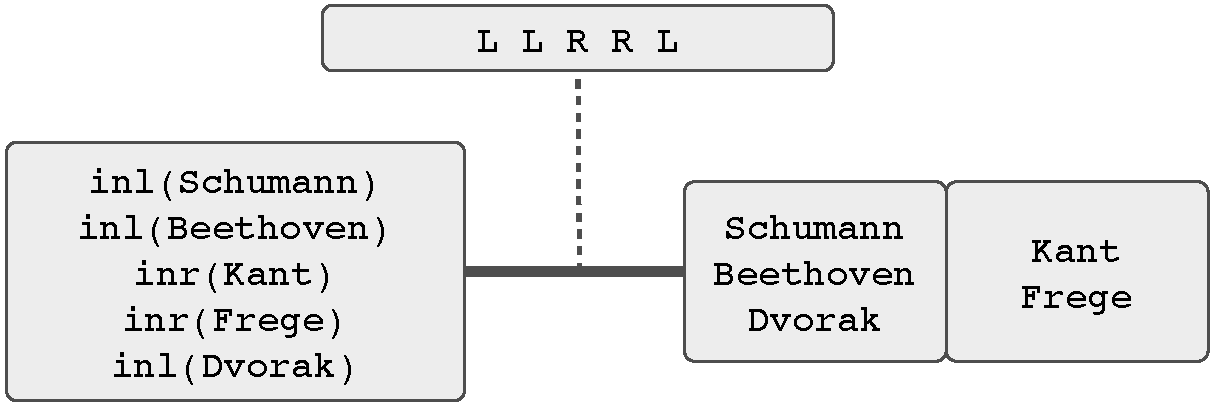
\includegraphics[width=75mm]{images/ex3-0.pdf}
        % \begin{tikzpicture}
        %     \draw
        %         node            (LSchumann)  {$\mlinl{\mbox{Schumann}}$}  (LSchumann)
        %         node[below=1ex] (LBeethoven) {$\mlinl{\mbox{Beethoven}}$} (LBeethoven)
        %         node[below=1ex] (LKant)      {$\mlinr{\mbox{Kant}}$}      (LKant)
        %         node[below=1ex] (LFrege)     {$\mlinr{\mbox{Frege}}$}     (LFrege)
        %         node[below=1ex] (LDvorak)    {$\mlinl{\mbox{Dvorak}}$}    (LDvorak)

        %         (LSchumann) +(7em, 0) node (CSchumann)  {$L$}
        %         (LBeethoven)+(7em, 0) node (CBeethoven) {$L$}
        %         (LKant)     +(7em, 0) node (CKant)      {$R$}
        %         (LFrege)    +(7em, 0) node (CFrege)     {$R$}
        %         (LDvorak)   +(7em, 0) node (CDvorak)    {$L$}

        %         (CKant)+(6.1em, 0)
        %         node            (RBeethoven) {Beethoven}
        %         node[above=1ex] (RSchumann)  {Schumann}
        %         node[below=1ex] (RDvorak)    {Dvorak}
        %         (RBeethoven)+(5em, 0) node {}
        %         node[above=0ex] (RKant)      {Kant}
        %         node[below=0ex] (RFrege)     {Frege}

        %         node[rbox,fit=(LDvorak) (LBeethoven) (LSchumann)]     (left)       {}
        %         node[rbox,fit=(CDvorak) (CSchumann)]                  (complement) {}
        %         node[rbox,fit=(RDvorak) (RSchumann) (RKant) (RFrege)] (right)      {}
        %         node[     fit=(RDvorak) (RBeethoven) (RSchumann)]     (right-inl)  {}
        %         node[     fit=(RKant) (RFrege)]                       (right-inr)  {}

        %         ($(right-inl.east)!0.5!(right-inr.west)$) node (right-center) {}
        %         (right-center |- right.north) -- (right-center |- right.south)

        %         node[below=2ex of complement]    (complement-label) {complement}
        %         (complement-label -| left)  node (left-label)       {left}
        %         (complement-label -| right) node (right-label)      {right}
        %     ;
        % \end {tikzpicture}
    \end{center}
    \caption{A consistent triple for the partition lens.}
    \label{fig:triple-partition}
    \vspace*{-2ex}
\end{figure}

As a warm-up, consider a simple edit: changing Dvorak's name to Dvo\v
r\'ak (with correct diacritics) in the left repository. The edit describing
this has the form \dissdis\mlmod5{\mlstayl{\d n}},\dissdis where $\d n$
describes the string edit to the
name. To translate this edit, we first need to 
translate the index $5$ to an index into the list of composers in the
right-hand repository (line \markref{rmodstay} in
Figure~\ifdissertation\ref{fig:definition-partition-part-2}\else\ref{fig:definition-partition}\fi).  We can do this by simply counting
how many composers 
appear up to and including Dvorak, that is, how many $L$ values appear in the
complement list up to index $5$---in this case, $3$.  We then wrap this
index up, along with the $\d n$ edit, in a new edit of the form
$\mlleft{\mlmod3{\d n}}$; the complement need not change because we
have not changed the structure of the lists. This pattern---count to
translate the index, then re-tag the edit appropriately---can be generalized
to all modifications that stay on the same side of the sum; the $\mlcount$
and $\mltag$ functions defined in
Figure~\ref{fig:definition-partition-supplementary} implement these two
steps.  

The left-to-right translation of other in-place modifications, insertions, and
deletions and the right-to-left translation of in-place modifications,
insertions, and deletions to either list are built from the same primitives, using
$\mlcount$ to translate indices and re-tagging edits with $\mltag$. 
%
In a few cases, we use some edit ``macros'': since insertions
and deletions always happen at the end of a list, we write $\mldelete'$ and
$\mlinsert'$ for edits that do some shuffling to ensure that the inserted or
deleted element moves to the appropriate position.

Perhaps the
most interesting of these is an in-place modification to the left repository
that switches sides of a sum (line~\markref{rmodswitch}).
%
For example, suppose we want to replace Beethoven with Plato. The edit to do
this has the form $\mlmod2{\mlswitch_{LR}(\d n)}$---that is, at position
$2$, switch from an $\mlinlx$ to an $\mlinrx$.  Here, the translated edit
must do \emph{four} things: delete Beethoven from the left list, insert a
new element into the right list, re-tag $\d n$ so that it changes the new
element to Plato, and finally fix up the complement to match the new
interleaving. As before, we can use $\mlcount$ to translate the position $2$
in the interleaved list into a position in the left list in the right
replica. But then we hit a minor snag: deletions only occur at the end of a
list. The solution is to first reorder the list, so that Beethoven appears
at the end, then delete one element.
Figure~\ref{fig:definition-partition-supplementary} defines the $\ml{cycle}$
function, which constructs permutations to do this reordering. The
function $\ml{cycle}_p(n)$ permutes lists of size $n$ by moving position $p$
to the end of the list, and shifting all the other elements after $p$ down
one to fill in the resulting hole. For example, $\ml{cycle}_2(5)$ looks like
this:
\begin{center}
    \begin{tabular}{c|ccccc}
        $p$ & $1$ & $2$ & $3$ & $4$ & $5$ \\
        \hline
        $\ml{cycle}_2(5)(p)$ & $1$ & $3$ & $4$ & $5$ & $2$
    \end{tabular}
\end{center}
So, we can delete position $p$ by first reordering with
$\mlreorder{\ml{cycle}_p}$, then deleting one element with $\mldel1$. The
$\mldelete'(p)$ macro encapsulates this pattern; there is a similar pattern for
inserting a new element at position $p$ encapsulated by $\mlinsert'(p)$.
Finally, since position $2$ in the interleaved list corresponds to positions
$2$ and $1$ in the left and right non-interleaved lists, respectively, the
final edit can be written as
$\mlright{\mlmod1{\d n}}\,\mlright{\mlinsert'(1)}\,\mlleft{\mldelete'(2)}$.
To fix up the complement, we can simply set the flag at position $p$ to
match the new tag: in our case, position $2$ is now an $\mlinrx$, so we
should set $c_2=R$.

% TODO: perhaps interesting: inserts to the right often have a free choice
% about where to insert on the left; discuss this?

The most delicate cases involve translating reorderings.
Consider an edit to the right repository that swaps Schumann and
Dvorak.  One way to write this edit is in terms of
a function that swaps 
indices one and three for lists of size at least three (and does nothing on
lists of size smaller than three):
\[f(n)(p) = \cond{
    4-p & n \ge 3 \land p \in \{1, 3\} \\
    p & n < 3 \lor p \notin \{1, 3\}
    }\]
The edit itself is then $\mlleft{\mlreorder f}$. Our job is now to compute
some $f'$ for which $\mlreorder{f'}$ swaps $\mlinl{\mbox{Schumann}}$ and
$\mlinl{\mbox{Dvorak}}$ in the left repository
(line~\markref{lreorder}). There is one wrinkle: $f$ 
and $f'$ are parameterized by the length of the lists they permute.
Translating $f$ naively would therefore seem to require a way for $f'$ to
\emph{guess}  the number of composers in lists whose lengths do not
match that of the complement. Fortunately,
$f'$ need only behave correctly for exactly those lists that are consistent
with the current complement, for which our ``guess'' about how many
composers there are is guaranteed to be accurate.  So 
we need only construct a single permutation (and use, say, the
identity permutation for all inconsistent list lengths).
%
We use the $\mlcount$ function to construct this permutation.
It is convenient to derive an isomorphism between positions in the left
repository and positions tagged by which list they are indexing into in the
right repository; the $\mliso$ function shows how to use $\mlcount$ to do
this. In our example, the resulting isomorphism looks like this:
\begin{center}
\noindent \begin{tabular}{c|ccccc}
    left  & $1$ & $2$ & $3$ & $4$ & $5$ \\
    \hline
    right & $\mlinl 1$ & $\mlinl 2$ & $\mlinr 1$ & $\mlinr 2$ & $\mlinl 3$
\end{tabular}
\end{center}

We can use $f(3)$ as a permutation on the $\mlinlx$ elements, defining%
\ifdissertation:
\[g(p) = \cond{\mlinr{p'} & p = \mlinr{p'} \\
               \mlinl{f(3)(p')} & p = \mlinl{p'}}\]
\else\ $g(\mlinl p)=\mlinl{f(3)(p)}$ and $g(\mlinr p)=\mlinr p$. \fi Then, to find out
where position $p$ in the left repository should come from, we can simply
translate $p$ into an index into the right repository using $\mliso$, apply
$g$ to find out where that index came from, and translate back into the left
repository using $\mliso^{-1}$. Expanding the table above with these
translations yields:
\begin{center}
\begin{tabular}{@{}c|ccccc@{}}
    left & $1$ & $2$ & $3$ & $4$ & $5$ \\
    \hline
    $\mliso$ & $\mlinl 1$ & $\mlinl 2$ & $\mlinr 1$ & $\mlinr 2$ & $\mlinl 3$ \\
    $\mliso;g$ & $\mlinl 3$ & $\mlinl 2$ & $\mlinr 1$ & $\mlinr 2$ & $\mlinl 1$ \\
    $\mliso;g;\mliso^{-1}$ & $5$ & $2$ & $3$ & $4$ & $1$
\end{tabular}
\end{center}
This swaps indices $1$ and $5$, so our final $f'$ looks like:
\[f'(n)(p) = \cond{
    6-p & n = 5 \land p \in \{1,5\} \\
    p & n \ne 5 \lor p \notin \{1,5\}
    }\]

Translating a reordering of the left repository follows a similar path (line~\markref{rreorder}):
restrict the reordering to lists consistent with the current complement,
then compose the permutation with isomorphisms between the indices in the
two repositories. There is one subtlety here: a reordering of the list
in the left repository may shuffle which positions are $\mlinlx$'s and which
are $\mlinrx$'s. As a result, we must take care to construct \emph{two}
separate position isomorphisms: one for ``before'' the reordering, and one
for ``after.''

% TODO: Somewhere in the above discussion we should probably try to give
% some intuition for what \mlcount does, since it's got such odd base cases.
% An attempt at English might go like this: Suppose we were to insert an L
% (respectively R) before index i in list c. How many Ls (respectively, Rs)
% would there be, up to this newly inserted item? These two numbers are the
% output of \mlcount(i,c).

\iffull
\begin{lemma}
    \label{lemma:unfold-mod-once}
    \[\mlmod p{\dv\CONS\dv s}z=\mlmod p\dv\mlmod p{\dv s}z\]
\end{lemma}

\begin{proof}
    Let $n=|z|$.  Either $p>n$ or not. If it is, then both sides are
    undefined; otherwise:
    \begin{align*}
        \mlmod p{\dv\CONS\dv s}z
            &= z[p \mapsto (\dv\CONS\dv s)z_p] \\
            &= z[p \mapsto \dv(\dv s\,z_p)] \\
            &= \mlmod p\dv(z[p \mapsto \dv s\,z_p]) \\
            &= \mlmod p\dv\mlmod p{\dv s}z
    \end{align*}
\end{proof}

\begin{lemma}
\label{lemma:high-level-delete}
If $1 \le p \le n$, then:
\[\mldelete'(p) \odot v = \blist v_1 \clist v_{p-1} \mlist v_{p+1} \clist v_n \elist\]
\end{lemma}

\begin{proof}
The only tricky part of this proof is evaluating $\ml{cycle}_p(n)$:
\begin{align*}
    \mldelete'(p) \odot v
        &= \blist\mldel 1\mlist\mlreorder{\ml{cycle}_p}\elist \odot v \\
        &= \blist\mldel 1\elist \odot \blist v_{\ml{cycle}_p(n)(1)} \clist v_{\ml{cycle}_p(n)(n)} \elist \\
        &= \blist\mldel 1\elist \odot \blist v_1 \clist v_{p-1} \mlist v_{p+1} \clist v_{n-1} \mlist v_p \elist \\
        &= \blist v_1 \clist v_{p-1} \mlist v_{p+1} \clist v_{n-1} \elist
\end{align*}
If $p=n$, then neither of the first two conditions in the definition of
$\ml{cycle}$ will ever be true, so $\ml{cycle}_p(n)(m)=m$, making the
evaluation given in these equations a special case where the interval from
$p+1$ to $n-1$ is empty and $v_p=v_n$. On the other hand, when $p<n$, the
value of $\ml{cycle}_p(n)$ is exactly in the form given here.
\end{proof}

\begin{lemma}
\label{lemma:high-level-insert}
When $1 \le p \le n+1$:
\[\mlinsert'(p) \odot \blist v_1 \clist v_n \elist =
    \blist v_1 \clist v_{p-1} \mlist \init \mlist v_p \clist v_n \elist\]
\end{lemma}

\begin{proof} Set $v_{n+1}=\init$ so that:
\begin{align*}
    \mlinsert'(p) \odot v_1 \cdots v_n
        &= \mlreorder{\lambda n.\ \ml{cycle}_p(n)^{-1}}\mlins 1 \odot \blist v_1 \clist v_n \elist \\
        &= \mlreorder{\lambda n.\ \ml{cycle}_p(n)^{-1}} \odot \blist v_1 \clist v_n\mlist\init\elist \\
        &= \mlreorder{\lambda n.\ \ml{cycle}_p(n)^{-1}} \odot \blist v_1 \clist v_{n+1} \elist \\
        &= \blist v_{\ml{cycle}_p(n+1)^{-1}(1)} \clist v_{\ml{cycle}_p(n+1)^{-1}(n+1)} \elist \\
        &= \blist v_1 \clist v_{p-1} \mlist v_{n+1} \mlist v_p \clist v_n \elist \\
        &= \blist v_1 \clist v_{p-1} \mlist \init \mlist v_p \clist v_n \elist
\end{align*}
As with Lemma~\ref{lemma:high-level-delete}, the only tricky part is arguing
that this evaluation of $\ml{cycle}_p$ is correct, and the argument is
similar to the one given there, but in reverse.
\end{proof}

\begin{lemma}
\label{lemma:lefts-rights-homomorphism}
The $\ml{lefts}$ and $\ml{rights}$ functions are list homomorphisms, that
is,
\[\ml{lefts}(vw)=\ml{lefts}(v)\ml{lefts}(w),\]
and similarly for $\ml{rights}$.
\end{lemma}

\begin{proof}
We will show the proof for $\ml{lefts}$. We argue by induction on $v$. In
the base case, $v=\NIL$, and:
\begin{align*}
    \ml{lefts}(vw)
        &= \ml{lefts}(w) \\
        &= \NIL\ml{lefts}(w) \\
        &= \ml{lefts}(\NIL)\ml{lefts}(w) \\
        &= \ml{lefts}(v)\ml{lefts}(w)
\end{align*}
Otherwise, $v=v_1 \CONS v'$, we know from the induction hypothesis that
$\ml{lefts}(v'w)=\ml{lefts}(v')\ml{lefts}(w)$, and by case analysis either
$v_1=\mlinl x$ or $v_1=\mlinr y$. In the former case:
\begin{align*}
    \ml{lefts}(vw)
        &= \ml{lefts}(\mlinl x \CONS v'w) \\
        &= x\CONS\ml{lefts}(v'w) \\
        &= x\CONS\ml{lefts}(v')\ml{lefts}(w) \\
        &= \ml{lefts}(\mlinl x \CONS v')\ml{lefts}(w) \\
        &= \ml{lefts}(v)\ml{lefts}(w)
\end{align*}
In the latter:
\begin{align*}
    \ml{lefts}(vw)
        &= \ml{lefts}(\mlinr y \CONS v'w) \\
        &= \ml{lefts}(v'w) \\
        &= \ml{lefts}(v')\ml{lefts}(w) \\
        &= \ml{lefts}(\mlinr y \CONS v')\ml{lefts}(w) \\
        &= \ml{lefts}(v)\ml{lefts}(w)
\end{align*}
\end{proof}

\begin{lemma}
\label{lemma:iso-coherent}
The isomorphism produced by $\mliso$ is coherent in the following sense.
Choose arbitrary $v\in(X+Y)\LIST$ and let $c=\map_{\ml{tagof}}(v)$ be
the list of tags of $v$. If $\mliso(c)(p)=\mlinl{p'}$ then
$\mlinl{\ml{lefts}(v)_{p'}}=v_p$ and likewise if $\mliso(c)(p)=\mlinr{p'}$
then $\mlinr{\ml{rights}(v)_{p'}}=v_p$.
\end{lemma}

\begin{proof}
Suppose there are $n_L$ copies of $L$ and $n_R$ copies of $R$ in $\blist c_1
\clist c_{p-1} \elist$ and $p \le n+1$. Then it is easy to show (by
induction on $c$) that $\ml{count}(p,\blist c_1 \clist c_n
\elist)=(1+n_L,1+n_R)$. Inspecting the definition of $\mliso$, it is
therefore clear that $\mliso(c)(p)=\mlinl{p'}$ exactly when $c_p=L$ and
there are $p'$ copies of $L$ in $\blist c_1 \clist c_p \elist$. This implies
there are exactly $p'$ elements tagged $\ml{inl}$ in $\blist v_1 \clist v_p
\elist$ (and that $v_p$ itself is tagged $\ml{inl}$), hence that
$\mlinl{\ml{lefts}(v)_{p'}}=v_p$.

The argument that $\mliso$ is coherent with $\ml{rights}$ is similar.
\end{proof}

\begin{corollary}
\label{lemma:iso-tag-index}
If $c=\map_{\ml{tagof}}(v)$ and $1 \le p \le |v|$, then
\[\ml{tagof}(v_p)=\ml{tagof}(\mliso(c)(p)).\]
\end{corollary}

\begin{lemma}
\label{lemma:iso-monotonic}
Suppose $\mliso(c)(m)=\mlinl n$ (respectively, $\mlinr n$) and
$\mliso(c)(m')=\mlinl{n'}$ (resp. $\mlinr{n'}$). Then $m<m'$ if and only if
$n<n'$.
\end{lemma}

\begin{proof}
    As shown in the proof of Lemma~\ref{lemma:iso-coherent}, we have
    $\mliso(c)(m)=\mlinl n$ exactly when $c_m=L$ and there are $n$ copies of
    $L$ in $\blist c_1 \clist c_m\elist$. A similar statement relates $m'$
    and $n'$. Since $\blist c_1 \clist c_m \elist$ and $\blist c_1 \clist
    c_{m'} \elist$ share a common prefix, if one has more copies of $L$ than
    the other then it must be longer---that is, $n'>n$ implies $m'>m$. On
    the other hand, since $c_m=c_{m'}=L$, if one is longer than the other
    than it definitely has more copies of $L$---that is, $m'>m$ implies
    $n'>n$.
\end{proof}

\begin{theorem}
The $\partition$ operation defined in \partitionfigures is indeed a
symmetric edit lens.
\label{goodlens:partition}
\end{theorem}

\begin{proof}
According to Definition~\ref{defn:lens}, we must show three things.  First,
$\partition.\dputr$ and $\partition.\dputl$ must be stateful monoid
homomorphisms; since the edit monoid for the list module is freely
generated and the two functions in question are defined by specification,
this is immediate.  Second, the initial state \[(\init_{(X \oplus
  Y)\LIST}, \NIL, \init_{X\LIST \otimes Y\LIST})\] must be an element of $K$;
this is easily verified from the definitions of the initial elements of the
list and product modules.  And third, the $\dputr$ and $\dputl$ operations
must preserve consistent states; this is where some work is required.  We
show that $\dputr\gen$ and $\dputl\gen$ respect $K$; since $\dputr$ and $\dputl$
are defined by specification from these, the fact that they respect $K$
follows by induction on the number of atomic edits they are handed.

\newcommand{\partitiondputrproof}{
We are given some $\dz \in G^{\mathrm{list}}_{X \oplus Y}$ such that
$\dz\;z$ is defined. We can define $(\dz',c')=\dputr\gen(\dz,c)$; then we
must show that $\dz'(x,y)$ is defined and that $(\dz\;z,c',\dz'(x,y)) \in
K$. We proceed by induction on the size of $\dz$.
\begin{trivlist}
\item {\bf Case \markref{rmodbigp}:}
    $\dv \in X \oplus Y$ and $\dz=\mlmod p\dv$ and $p > |c|$.

    \noindent
    Since $|z|=|c|$, we conclude that $\dz\;z$ is undefined, a
    contradiction.

\item {\bf Case \markref{rmodempty}:}
    $\dz=\mlmod p\NIL$ and $1 \le p \le |c|$.

    \noindent
    We calculate:
    \begin{align*}
        \dz' &= \NIL \\
        c' &= c \\
        \dz\;z &= z \\
        \dz'(x,y) &= (x,y)
    \end{align*}
    So $(\dz\;z,c',\dz'(x,y)) \in K$ by assumption:
    $(z,c,(x,y)) \in K$.

\item {\bf Case \markref{rmodcons}:}
    We have all of the following:
    \begin{align}
        \dv &\in G^\oplus_{X,Y} \\
        \dv s &\in \D(X\oplus Y) \\
        \dz &= \mlmod p{\dv\CONS\dv s} \\
        1 &\le p \le |c| \\
        1 &< n \\
        (d,c'') &= \dputr\gen(\mlmod p{\dv s},c) \label{eq:IH-1} \\
        (d',c') &= \dputr\gen(\mlmod p\dv,c'') \label{eq:IH-2} \\
        \dz' &= d'\;d
    \end{align}
    By Lemma~\ref{lemma:unfold-mod-once} and the assumption that $\mlmod
    p{\dv\CONS\dv s}z$ is defined, we know $\mlmod p\dv(\mlmod p{\dv s}z)$ is
    defined, and hence $\mlmod p{\dv s}z$ is defined. The induction
    hypothesis for equation~\ref{eq:IH-1} therefore tells us that $d\;(x,y)$
    is defined and that
    \[(\mlmod p{\dv s}z,c'',d\;(x,y)) \in K.\]
    Again appealing to the induction hypothesis, this time for
    equation~\ref{eq:IH-2}, we also know that $d'\;(d\;(x,y))$ is defined and
    \[(\mlmod p\dv(\mlmod p{\dv s}z),c',d'\;(d\;(x,y))) \in K.\]
    By one final appeal to Lemma~\ref{lemma:unfold-mod-once}, we therefore
    conclude that
    \[(\dz\;z,c',\dz'(x,y)) \in K\]
    as desired.

\item {\bf Case \markref{rmodswitch}:}
    We have:
    \begin{align*}
        \dz &= \mlmod p{\mlswitch_{jk}(\dv)} \\
        1 &\le p \le |c| \\
        \dv &\in \partial X\mbox{ when }k = L \\
        \dv &\in \partial Y\mbox{ when }k = R \\
        \dz' &= d_2d_1d_0 \\
        c' &= c[p \mapsto k] \\
        d_0 &= \map_{\lambda d.\,\ml{tag}(j,d)}(\mldelete'(p_j)) \\
        d_1 &= \map_{\lambda d.\,\ml{tag}(k,d)}(\mlinsert'(p_k)) \\
        d_2 &= \ml{tag}(k,\mlmod{p_k}\dv) \\
        (p_L,p_R) &= \mlcount(p,c)
    \end{align*}
    Let us consider the case when $j=k=L$, whose argument is representative
    of the other cases.

    Since $\dz\;z$ is defined, we know that $z_p = \mlinl v$ for some $v \in
    X$. Taking $v'=\dv\;\init_X$, we can now compute:
    \begin{align*}
        \map_{\ml{tagof}}(\dz\;z)
            &= \map_{\ml{tagof}}(z[p\mapsto\mlinl{v'}]) \\
            &= \map_{\ml{tagof}}(\blist z_1\clist z_{p-1}\elist)\;
               \blist k\elist\;
               \map_{\ml{tagof}}(\blist z_{p+1}\clist z_n\elist)\\
            &= \blist c_1\clist c_{p-1}\mlist k\mlist c_{p+1}\clist c_n \elist\\
            &= c[p \mapsto k] \\
            &= c'
    \end{align*}
    The second line follows from the first because \map is a list
    homomorphism.  Hence $\dputr\gen$ maintains consistency of $c$ in this
    case; it remains to show that $\dputr\gen$ maintains consistency of the
    output. We calculate the effects of $\dz$ and $\dz'$, starting with
    $\dz'$:
    \begin{align*}
        \dz'\;(x,y)
            &= d_2d_1d_0(x,y) \\
            &= d_2d_1(\map_{\lambda d.\ml{tag}(j,d)}(\mldelete'(p_j)))(x,y) \\
            &= d_2d_1(\map_{\ml{left}}(\mldelete'(p_L)))(x,y) \\
            &= d_2d_1(\mldelete'(p_L)x,y) \\
            &= d_2(\map_{\lambda d.\ml{tag}(k,d)}(\mlinsert'(p_k)))(\mldelete'(p_L)x,y) \\
            &= d_2(\map_{\ml{left}}(\mlinsert'(p_L)))(\mldelete'(p_L)x,y) \\
            &= d_2(\mlinsert'(p_L)\mldelete'(p_L)x,y) \\
            &= \mltag(k,\mlmod(p_k,\dv))(\mlinsert'(p_L)\mldelete'(p_L)x,y) \\
            &= (\mlmod{p_L}\dv\mlinsert'(p_L)\mldelete'(p_L)x,y)
    \end{align*}
    We can use Lemmas~\ref{lemma:high-level-delete}
    and~\ref{lemma:high-level-insert} to simplify:
    \begin{align*}
        \dz'\;(x,y)
            &= (\mlmod{p_L}\dv\mlinsert'(p_L)\mldelete'(p_L)\blist x_1\clist x_{n_L}\elist,y) \\
            &= (\mlmod{p_L}\dv\mlinsert'(p_L)\blist x_1\clist x_{p_L-1}\mlist x_{p_L+1}\clist x_{n_L}\elist,y) \\
            &= (\mlmod{p_L}\dv\blist x_1\clist x_{p_L-1}\mlist\init_X\mlist x_{p_L+1}\clist x_{n_L}\elist,y) \\
            &= (\blist x_1\clist x_{p_L-1}\mlist v'\mlist x_{p_L+1}\clist x_{n_L}\elist,y) \\
            &= (x[p_L\mapsto v'], y)
    \end{align*}
    We now make some observations about the effects of $\dz$, making crucial
    use of Lemma~\ref{lemma:lefts-rights-homomorphism}:
    \begin{align*}
        \ml{rights}(\dz\;z)
            &= \ml{rights}(\blist z_1 \clist z_{p-1} \mlist \mlinl{v'} \mlist z_{p+1} \clist z_n \elist) \\
            &= \ml{rights}(\blist z_1 \clist z_{p-1}\elist) \ml{rights}(\mlinl{v'}) \ml{rights}(\blist z_{p+1} \clist z_n \elist) \\
            &= \ml{rights}(\blist z_1 \clist z_{p-1}\elist) \ml{rights}(\mlinl{v}) \ml{rights}(\blist z_{p+1} \clist z_n \elist) \\
            &= \ml{rights}(\blist z_1 \clist z_{p-1}\elist) \ml{rights}(z_p) \ml{rights}(\blist z_{p+1} \clist z_n \elist) \\
            &= \ml{rights}(\blist z_1 \clist z_{p-1} \mlist z_p \mlist z_{p+1} \clist z_n \elist) \\
            &= \ml{rights}(z) \\
            &= y
    \end{align*}
    We now observe that Lemma~\ref{lemma:iso-coherent} implies that
    $\ml{lefts}(\blist z_1 \clist z_{p-1} \elist)=\blist x_1 \clist
    x_{p_L-1} \elist$ and likewise that $\ml{lefts}(\blist z_{p+1} \clist
    z_n \elist)=\blist x_{p_L+1} \clist x_{n_L} \elist$.
    \begin{align*}
        \ml{lefts}(\dz\;z)
            &= \ml{lefts}(z[p \mapsto \mlinl{v'}]) \\
            &= \ml{lefts}(\blist z_1 \clist z_{p-1} \elist)\ml{lefts}(\mlinl{v'})\ml{lefts}(\blist z_{p+1} \clist z_n \elist) \\
            &= \blist x_1\clist x_{p_L-1}\mlist v'\mlist x_{p_L+1}\clist x_{n_L}\elist \\
            &= x[p_L\mapsto v']
    \end{align*}
    Taken together, these last three computations show that
    \[\dz'\;(x,y) = (\ml{lefts}(\dz\;z),\ml{rights}(\dz\;z))\]
    which is just what we needed.

\item {\bf Case \markref{rmodstay}:} Let us consider specifically the case
    where $j=L$; the argument for $j=R$ is very similar. Then we have
    \begin{align*}
        \dz &= \mlmod p{\mlstayl\dv} \\
        \dz' &= \mlonl{\mlmod{p_L}\dv} \\
        (p_L,p_R) &= \mlcount(p,c)
    \end{align*}
    Moreover, since $\dz\;z$ is defined, we know that there is some $v \in
    X$ for which $\dv\;v$ is defined such that $z_p = \mlinl v$ and, by
    appeal to Lemma~\ref{lemma:iso-coherent}, we know in particular that
    $v=\ml{lefts}(z)_{p_L}=x_{p_L}$. Hence $\dz'\;(x,y)$ is defined.

    We now observe that $\mlmod p{\mlstayl\dv}$ does not change any tags or
    any non-$\ml{inl}$ values, so $\map_{\ml{tagof}}(\dz\;z) =
    \map_{\ml{tagof}}(z) = c$ and $\ml{rights}(\dz\;z) = \ml{rights}(z)
    = y$. Furthermore:
    \begin{align*}
        \ml{lefts}(\dz\;z)
        &= \ml{lefts}(\mlmod p{\mlstayl\dv}\;z[p \mapsto \mlinl{x_{p_L}}]) \\
        &= \ml{lefts}(z[p\mapsto\mlinl{\dv\;x_{p_L}}]) \\
        &= x[p_L\mapsto \dv\;x_{p_L}] \\
        &= \mlmod{p_L}{\dv}\;x
    \end{align*}
    That is, $\dz\;z$ and $\dz'\;(x,y)=(\mlmod{p_L}\dv\;x,y)$ are synchronized as desired.

\item {\bf Case \markref{rmodfail}:}
    When $\dz=\mlmod p\fail$ there is nothing to prove, because the
    assumption that the edit application is defined is immediately
    contradicted.

\item {\bf Case \markref{rins}:}
    \begin{align*}
        \dz &= \mlins i \\
        \dz' &= \mlonl{\mlins i}  \\
        c' &= \mlins i\,c
    \end{align*}

    \noindent
    We calculate:
    \begin{align*}
        \dz\;z &= z\replicate i{\init_{X\oplus Y}}
\\
               &= z\replicate i{\mlinl{\init_X}}
\\
        \dz'(x,y) &= (x\replicate i{\init_X},\, y)
\\
        c' &= c\replicate iL
    \end{align*}
    Now, since \map is a list homomorphism, we have:
    \begin{align*}
        \map_\ml{tagof}(\dz\;z)
            &= \map_\ml{tagof}(z)\map_\ml{tagof}\left(\replicate i{\mlinl{\init_X}}\right) \\
            &= c\replicate iL \\
            &= c'
    \end{align*}
    Likewise, by Lemma~\ref{lemma:lefts-rights-homomorphism}:
    \begin{align*}
        \ml{lefts}(\dz\;z)
            &= \ml{lefts}(z)\ml{lefts}\left(\replicate i{\mlinl{\init_X}}\right) \\
            &= x\replicate i{\init_X} \\
        \ml{rights}(\dz\;z)
            &= \ml{rights}(z)\ml{rights}\left(\replicate i{\mlinl{\init_X}}\right) \\
            &= y
    \end{align*}
    These latter two computations amount to showing that
    \dissdis\dz'(x,y)=(\ml{lefts}(\dz\;z),\ml{right}(\dz\;z))\dissdis which, together with
    the observation above that $\map_\ml{tagof}(\dz\;z)=c'$, shows that
    $\dputr\gen$ preserves consistency in this case.

\item {\bf Case \markref{rdel}:}
    \begin{align*}
        \dz &= \mldel i \\
        \dz' &= \mlright{\mldel{n_L-1}}\mlleft{\mldel{n_R-1}} \\
        (n_L,n_R) &= \mlcount(i+1,\mlreverse(c))
    \end{align*}
    (Take careful notice of the definition of $n_L$ and $n_R$ here: it
    differs from the convention established at the beginning of the proof!
    We will use these local definitions for the remainder of this case.)

    The interesting thing to prove is that $\ml{lefts}(\mldel i\;z) =
    \mldel{n_L-1}\ml{lefts}(z)$ (and similarly for $\ml{rights}$). We
    proceed by an inner induction on $i$.

    When $i=0$, we have $\ml{lefts}(\mldel 0\;z)=\ml{lefts}(z)$ and
    \[(n_L,n_R) = \mlcount(1,\mlreverse(c)) = (1,1)\] so that
    $\mldel{n_L-1}\ml{lefts}(z)=\mldel0\ml{lefts}(z)=\ml{lefts}(z)$.

    Suppose $i>0$. Define the abbreviation $c^r=\mlreverse(c)$.
    Then the induction hypothesis says that
    \[\ml{lefts}(\mldel{i-1}\;z)=\mldel{\mlfst(\mlcount(i,c^r))-1}\ml{lefts}(z).\]
    Now, either $c^r_i=L$ or $c^r_i=R$. If the former, then
    $z_{n-i+1}=\mlinl x$ for some $x$ and:
    \begin{align*}
        \mldel{n_L-1}\ml{lefts}(z)
        &= \mldel{\mlfst(\mlcount(i+1,c^r))-1}\ml{lefts}(z) \\
        &= \mldel{1+\mlfst(\mlcount(i,c^r))-1}\ml{lefts}(z) \\
        &= \mldel1\mldel{\mlfst(\mlcount(i,c^r))-1}\ml{lefts}(z) \\
        &= \mldel1\ml{lefts}(\mldel{i-1}\;z) \\
        &= \mldel1\ml{lefts}(\blist z_1 \clist z_{n-i}\mlist\mlinl x\elist) \\
        &= \mldel1(\ml{lefts}(\blist z_1 \clist z_{n-i}\elist)x) \\
        &= \ml{lefts}(\blist z_1 \clist z_{n-i}\elist) \\
        &= \ml{lefts}(\mldel i\;z)
    \end{align*}
    Otherwise, $z_{n-i+1}=\mlinr y$ for some $y$ and:
    \begin{align*}
        \mldel{n_L-1}\ml{lefts}(z)
        &= \mldel{\mlfst(\mlcount(i+1,c^r))-1}\ml{lefts}(z) \\
        &= \mldel{\mlfst(\mlcount(i,c^r))-1}\ml{lefts}(z) \\
        &= \ml{lefts}(\mldel{i-1}\;z) \\
        &= \ml{lefts}(\blist z_1 \clist z_{n-i}\mlist\mlinr y\elist) \\
        &= \ml{lefts}(\blist z_1 \clist z_{n-i}\elist) \\
        &= \ml{lefts}(\mldel i\;z)
    \end{align*}
    as desired.

    A similar argument shows that:
    \[\ml{rights}(\mldel i\;z) = \mldel{n_R-1}\ml{rights}(z)\]

\item {\bf Case \markref{rreorder}:}
    The main idea of the proof for this case is to observe that $c$ contains
    enough information to deduce the length of $x$, $y$, and $z$, and in
    particular which index the various $\ml{reorder}$ edits will be
    specialized to during edit application. We can focus on these indices.
    (We will see that the somewhat strange-looking clause defining $f_k(n
    \ne n_k) = \lambda p.\; p$ is never used -- the lens could use any
    automorphism on $\{1,\ldots,n\}$ in place of the identity there.)

    Because the application of $\dz$ and $\dz'$ are always defined, we need
    only show that the new complement and the output edits are consistent
    with the input edits. We begin by showing the new complement is
    consistent with $\dz\;z$.

    \begin{align}
        \map_{\ml{tagof}}(\dz\;z)
            &= \map_{\ml{tagof}}(\blist z_{f(n)(1)}\clist z_{f(n)(n)}\elist)
            \label{eq:reorder-z} \\
            &= \blist\map_{\ml{tagof}}(z)_{f(n)(1)}\clist\map_{\ml{tagof}}(z)_{f(n)(n)}\elist
            \label{eq:float-index} \\
            &= \blist c_{f(n)(1)} \clist c_{f(n)(n)} \elist
            \label{eq:def-c} \\
            &= \mlreorder f\;c
            \label{eq:def-reorder}
    \end{align}

    Equation~\ref{eq:reorder-z} follows by definition of edit application in
    the list module (and because $|z|=|c|=n$); equation~\ref{eq:float-index}
    is a special property of \map; equation~\ref{eq:def-c} by
    definition of $c$; and equation~\ref{eq:def-reorder} by the definition
    of $\ml{reorder}$'s edit application.

    We will now show that $\ml{lefts}(\dz\;z)=\mlreorder{f_L}\;x$. A similar
    argument to the following also shows that
    $\ml{rights}(\dz\;z)=\mlreorder{f_R}\;y$, and these two facts together
    will conclude the proof (since
    $\dz'\;(x,y)=(\mlreorder{f_L}\;x,\mlreorder{f_R}\;y)$). By the above
    fact about $c'$ and Lemma~\ref{lemma:iso-coherent}:
    \begin{align}
        \mlinl{\ml{lefts}(\dz\;z)_i}
            &= (\dz\;z)_{\mliso^{-1}(c')(\mlinl i)}
            \label{eq:lefts-lemma}\\
            &= (\dz\;z)_{h'^{-1}(\mlinl i)}
            \label{eq:def-h'}\\
            &= z_{f(n)(h'^{-1}(\mlinl i))}
            \label{eq:apply-reordering-to-def-h'}\\
            &= \mlinl{\ml{lefts}(z)_{\mluntag(\mliso(c)(f(n)(h'^{-1}(\mlinl i))))}}
            \label{eq:lefts-unlemma}\\
            &= \mlinl{\ml{lefts}(z)_{\mluntag(h(f(n)(h'^{-1}(\mlinl i))))}}
            \label{eq:def-h}\\
            &= \mlinl{\ml{lefts}(z)_{(\ml{inl};h'^{-1};f(n);h;\mluntag)(i)}}
            \label{eq:semi-syntax}\\
            &= \mlinl{\ml{lefts}(z)_{(\ml{inl};h'';\mluntag)(i)}}
            \label{eq:def-h''}\\
            &= \mlinl{\ml{lefts}(z)_{f_L(n_L)(i)}}
            \label{eq:def-fL}\\
        \ml{lefts}(\dz\;z)_i &= \ml{lefts}(z)_{f_L(n_L)(i)}
            \label{eq:uninl}
    \end{align}
    Equation~\ref{eq:lefts-lemma} is a straightforward application of
    Lemma~\ref{lemma:iso-coherent}; equation~\ref{eq:def-h'} folds the
    definition of $h'$; and equation~\ref{eq:apply-reordering-to-def-h'} applies
    edit $\dz$. Equation~\ref{eq:lefts-unlemma} applies
    Lemma~\ref{lemma:iso-coherent} again, but with the knowledge that the
    tag of the previous line is $\ml{inl}$ (because that is the left-hand
    side of the equality we have already proved). Equations~\ref{eq:def-h},
    \ref{eq:semi-syntax}, \ref{eq:def-h''}, and~\ref{eq:def-fL} just rewrite
    the equation by folding the definitions of $h$, $h''$, and $f_L$ and
    rewriting explicit function application as the application of a function
    composition. The final equation~\ref{eq:uninl} holds by injectivity of
    $\ml{inl}$.

    Now, since $x=\ml{lefts}(z)$ and $|x|=n_L$, we can conclude that
    $\ml{lefts}(\dz\;z)=\mlreorder{f_L}\;x$ as desired.

\item {\bf Case \markref{rfail}:} As in Case~\markref{rmodfail}, there is
    nothing to prove, as the assumption that the edit application is defined
    is immediately contradicted.

\end{trivlist}
}
\newcommand{\partitiondputlproof}{
We will give the proofs for atomic edits of the form $\mlonl\dx$; the proofs
for edits of the form $\mlonr\dy$ are similar. Choose $\dx \in
G^{\mathrm{list}}_X$ such that $\dx\;x$ is defined. We define
$(\dz,c')=\dputl\gen(\mlonl\dx,c)$ and must show that $\dz\;z$ is defined and
that $(\dz\;z,c',(\dx\;x,y)) \in K$. We proceed by induction on the size of
$\dx$.

\begin{trivlist}

\item {\bf Case \markref{lmod}:} In this case, we have the following
    equalities:
    \begin{align*}
        \dx &= \mlmod p\dv \\
        \dz &= \mlmod{p'}{\mlstayl\dv} \\
        c' &= c \\
        p' &= \mliso(c)^{-1}(\mlinl p)
    \end{align*}
    By Lemma~\ref{lemma:iso-coherent},
    $z_{p'}=\mlinl{\ml{lefts}(z)_p}=\mlinl{x_p}$. This gives us enough to
    know that $\dz\;z$ is defined and in fact that
    \begin{align*}
        \dz\;z
            &= z[p' \mapsto \mlstayl\dv\;z_{p'}] \\
            &= z[p' \mapsto \mlstayl\dv\;\mlinl{x_p}] \\
            &= z[p' \mapsto \mlinl{\dv\;x_p}]
    \end{align*}
    Since none of the tags of $z$ changes during this operation, this makes
    the computation of $\ml{lefts}$, $\ml{rights}$, and $\map_{\ml{tagof}}$
    easy:
    \begin{align*}
        \map_{\ml{tagof}}(\dz\;z)
            &= \map_{\ml{tagof}}(z) \\
            &= c \\
            &= c' \\
        \ml{rights}(\dz\;z)
            &= \ml{rights}(z) \\
            &= y \\
        \ml{lefts}(\dz\;z)
            &= \ml{lefts}(z)[p \mapsto \dv\;x_p] \\
            &= x[p \mapsto \dv\;x_p] \\
            &= \dx\;x
    \end{align*}
    These three computations establish that $(\dz\;z,c',(\dx\;x,y)) \in K$,
    as desired.

\item {\bf Case \markref{lreorder}:} We have a slew of equalities in hand to
    begin with. We have some chosen $f$ and three main equalities:
    \begin{align*}
        \dx &= \mlreorder f \\
        \dz &= \mlreorder{f'} \\
        c' &= c
    \end{align*}
    These depend on the additional definitions:
    \begin{align*}
        g(\mlinr p) &= \mlinr p &
        f'(n \ne |c|) &= \lambda p.\,p \\
        g(\mlinl p) &= \mlinl{f(n_L)(p)} &
        f'(|c|) &= h;g;h^{-1} \\
        h &= \mliso(c)
    \end{align*}

    We first observe that $\mlreorder{f'}$ does not affect tags at all. To
    be precise, for $1 \le p \le n$, we have:
    \begin{align}
        \ml{tagof}((\mlreorder{f'}\;z)_p)
            &= \ml{tagof}(z_{(h;g;h^{-1})(p)})
            \label{eq:def-reorder-f} \\
            &= \ml{tagof}((h;g;h^{-1};h)(p))
            \label{eq:swap-index-to-iso} \\
            &= \ml{tagof}((h;g)(p))
            \label{eq:elim-iso} \\
            &= \ml{tagof}(h(p))
            \label{eq:inspect-g} \\
            &= \ml{tagof}(z_p)
            \label{eq:swap-iso-to-index}
    \end{align}
    Equation~\ref{eq:def-reorder-f} follows from the definition of $f'$ and
    edit application. Equation~\ref{eq:swap-index-to-iso} is an application
    of Corollary~\ref{lemma:iso-tag-index}; we can then simplify
    significantly in equations~\ref{eq:elim-iso} and~\ref{eq:inspect-g}
    because $h$ is an isomorphism and $g$ does not modify tags, as is
    evident from its definition. A second application of
    Corollary~\ref{lemma:iso-tag-index}, this time ``in reverse'', gives us
    the final equation~\ref{eq:swap-iso-to-index}. We conclude that
    \[\map_{\ml{tagof}}(\dz\;z) = \map_{\ml{tagof}}(z) = c = c',\]
    part of what we need to show that $(\dz\;z,c',(\dx\;x,y))\in K$. (It
    also means that $h$ is the appropriate isomorphism to use when applying
    Lemma~\ref{lemma:iso-coherent} to $\dz\;z$.)

    Let us now turn our attention to showing that $\dz\;z$ and $\dx\;x$ have
    the appropriate relationship. We reason as follows:
    \begin{align}
        \mlinl{\ml{lefts}(\dz\;z)_p}
            &= (\dz\;z)_{h^{-1}(\mlinl p)}          \label{eq:lreorder-x-iso} \\
            &= z_{(h^{-1};h;g;h^{-1})(\mlinl p)}    \label{eq:lreorder-x-reorder} \\
            &= z_{(g;h^{-1})(\mlinl p)}             \label{eq:lreorder-x-elim-iso} \\
            &= z_{h^{-1}(f(n_L)(p))}                \label{eq:lreorder-x-g} \\
            &= \mlinl{\ml{lefts}(z)_{f(n_L)(p)}}    \label{eq:lreorder-x-iso2}
    \end{align}
    Equation~\ref{eq:lreorder-x-iso} is an application of
    Lemma~\ref{lemma:iso-coherent}. The next three equations,
    \ref{eq:lreorder-x-reorder} through \ref{eq:lreorder-x-g}, are mere
    computations that invoke the definitions of $\dz$, edit application, and
    $g$. The final equation~\ref{eq:lreorder-x-iso2} follows from the
    previous by Lemma~\ref{lemma:iso-coherent}. A similar argument to the
    above, differing only in line~\ref{eq:lreorder-x-g} where the definition
    of $g$ is used, shows that
    \[\mlinr{\ml{rights}(\dz\;z)_p} = \mlinr{\ml{rights}(z)_p}.\]

    We can therefore conclude that $\ml{lefts}(\dz\;z) = \dx\;\ml{lefts}(z)
    = \dx\;x$ and that $\ml{rights}(\dz\;z) = \ml{rights}(z) = y$, that is,
    that $(\dz\;z,c',(\dx\;x,y))\in K$ as desired.

\item {\bf Case \markref{lins}:} We know $\dx = \mlins i$ and $\dz = \mlins
    i$ and $c' = \mlins i\; c$. We compute:
    \begin{align*}
        \map_{\ml{tagof}}(\dz\;z)
            &= \map_{\ml{tagof}}(z \replicate i{\init_{X \oplus Y}}) \\
            &= \map_{\ml{tagof}}(z)\map_{\ml{tagof}}(\replicate i{\init_{X \oplus Y}}) \\
            &= c\replicate iL \\
            &= \mlins i\;c \\
            &= c'
    \end{align*}
    There's a slight left-bias here; in the right- version of this proof, we
    find that $\dputl\gen$ would have to produce a $c'$ with many replicated
    $R$s instead of $L$s, and so would not have quite as compact a syntax
    for this output.
    % TODO: does this mean we should explicitly give \dputl\gen(\mlonr{\mlins
    % i}) when defining the partition lens above?

    \begin{align*}
        \ml{lefts}(\dz\;z)
            &= \ml{lefts}(z\replicate i{\init_{X \oplus Y}}) \\
            &= \ml{lefts}(z)\ml{lefts}(\replicate i{\init_{X \oplus Y}}) \\
            &= x\replicate i{\init_X} \\
            &= \mlinsert(i)\;x \\
            &= \dx\;x
    \end{align*}
    Again, the left-bias means the right- version of this proof relies on
    $\dputl\gen$ being slightly more complicated for the right- analog. In
    particular, $\dputl\gen$ would need to output an edit which did the
    insertion above followed by a series of modifications that turned the
    $i$ final copies of $\mlinl{\init_X}$ into $i$ copies of
    $\mlinr{\init_Y}$.

    A similar computation to the previous one shows that
    $\ml{rights}(\dz\;z)=\ml{rights}(z)=y$.
%
    This concludes the proof of this case, since our three computations have
    shown that $(\dz\;z,c',(\dx\;x,y)) \in K$.

\item {\bf Case \markref{ldel0}:} We have $\dx = \mldel 0$ and $\dz = \NIL$
    and $c' = c$. Since $\dz\;z=z$, $\dx\;x=x$, and $c'=c$,
    we are in the happy situation of having assumed exactly what we need to
    prove, namely that $(\dz\;z,c',(\dx\;x,y))=(z,c,(x,y)) \in K$.

\item {\bf Case \markref{ldeli}:} To fit in with the surrounding
    conventions in the proof, we will rename a few of the bindings
    of this case. To be specific, we have
    \begin{align*}
        \dx &= \mldel i \\
        \dz &= d'd \\
        (d',c') &= \dputl\gen(d'',c'') \\
        d'' &= \mlonl{\mldel{i-1}} \\
        c'' &= d\;c \\
        d &= \mldelete'(\mliso(c)^{-1}(\mlinl{n_L}))
    \end{align*}
    and we know that $1 \le i \le n_L$. Our strategy is to show that
    $(d\;z,c'',(\mldel1\;x,y)) \in K$; the induction hypothesis then
    tells us that $(d'\;(d\;z),c',d''\;(\mldel1\;x,y))\in K$. This means
    that $((d'd)\;z,c',(\mldel i\;x,y)) \in K$, which concludes this case.
    In the remainder of this case, let $m=\mliso(c)^{-1}(\mlinl{n_L})$ so
    that $d=\mldelete'(m)$.

    Let us begin by showing that $\map_{\ml{tagof}}(d\;z)=d\;c$. Then
    Lemma~\ref{lemma:high-level-delete} tells us two things:
    \begin{align*}
        d\;z &= \blist z_1 \clist z_{m-1} \mlist z_{m+1} \clist z_n \elist \\
        d\;c &= \blist c_1 \clist c_{m-1} \mlist c_{m+1} \clist c_n \elist
    \end{align*}
    The desired equality then follows from the fact that $\map$ is a list
    homomorphism and that $\map_{\ml{tagof}}(z)=c$.

    We must also show that $\ml{lefts}(d\;z)=\mldel1\;x$. By
    Lemma~\ref{lemma:iso-coherent}, $z_m=\mlinl{x_{n_L}}$, and by
    Lemma~\ref{lemma:iso-monotonic}, $z_{m'}$ is an $\mlinrx$ for all
    $m'>m$. Since $\ml{lefts}$ is a list homomorphism, we can conclude that
    \begin{align*}
        \ml{lefts}(d\;z) &=
            \ml{lefts}(\blist z_1 \clist z_{m-1} \mlist z_{m+1} \clist z_n \elist)
        \\ &=
            \ml{lefts}(\blist z_1 \clist z_{m-1} \elist)\;
            \ml{lefts}(\blist z_{m+1} \clist z_n \elist)
        \\ &=
            \ml{lefts}(\blist z_1 \clist z_{m-1} \elist)
        \\ &=
            \mldel1\;(\ml{lefts}(\blist z_1 \clist z_{m-1} \elist)\;
                      \ml{lefts}(\blist \mlinl{x_{n_L}} \elist))
        \\ &=
            \mldel1\;(\ml{lefts}(\blist z_1 \clist z_{m-1} \elist)\;
                      \ml{lefts}(\blist \mlinl{x_{n_L}} \elist)\;
                      \ml{lefts}(\blist z_{m+1} \clist z_n \elist))
        \\ &=
            \mldel1\;(\ml{lefts}(z))
        \\ &=
            \mldel1\;x
    \end{align*}
    as desired.

    Next, we show that $\ml{rights}(d\;z)=y$. By
    Lemma~\ref{lemma:iso-coherent}, we know $z_m=\mlinl{x_{n_L}}$. Since
    $\ml{rights}$ is a list homomorphism and $\ml{rights}(\mlinl v)=\NIL$
    for any $v$, we then can compute that:
    \begin{align*}
        \ml{rights}(d\;z) &=
            \ml{rights}(\blist z_1 \clist z_{m-1} \mlist z_{m+1} \clist z_n \elist)
        \\ &=
            \ml{rights}(\blist z_1 \clist z_{m-1} \elist)\;
            \ml{rights}(\blist z_{m+1} \clist z_n \elist)
        \\ &=
            \ml{rights}(\blist z_1 \clist z_{m-1} \elist)\;
            \ml{rights}(\blist \mlinl{x_{n_L}} \elist)\;
            \ml{rights}(\blist z_{m+1} \clist z_n \elist)
        \\ &=
            \ml{rights}(\blist z_1 \clist z_{m-1} \mlist z_m \mlist z_{m+1} \clist z_n \elist)
        \\ &=
            \ml{rights}(z)
        \\ &=
            y
    \end{align*}

    The previous three paragraphs establish that $(d\;z, c'',
    (\mldel1\;x, y)) \in K$. Since $d''=\mlonl{\mldel{i-1}}$ is a smaller
    edit than $\mlonl\dx=\mlonl{\mldel i}$, we can apply the induction
    hypothesis to conclude that $(d'\;(d\;z), c', d''\;(\mldel1\;x, y)) \in
    K$. Since edit application is a monoid action, we know
    $d'\;(d\;z)=(d'd)\;z$. By definition of the edit application, we know
    $d''\;(\mldel1\;x,y)=(\mldel{i-1}\;(\mldel1\;x),y)=(\mldel i\;x,y)$.
    These last two equalities directly mean that $(\dz\;z,c',(\dx\;x,y)) \in
    K$, which completes this case.

\item {\bf Case \markref{ldelfail}:} We know $\dx=\mldel i$ and, since the
    previous cases did not apply, $i>n_L+1$. Hence we know $\dx\;x$ is not
    defined, a contradiction to our assumption that it is.

\item {\bf Case \markref{lfail}:} Since $\dx=\fail$, the assumption that
    $\dx$ successfully applies is immediately contradicted, so there is
    nothing to prove in this case.

\end{trivlist}
}

For the two parts of the proof that follow, choose some $(z,c,(x,y)) \in K$.
We will define $n=|z|$, $n_L=|x|$, and $n_R=|y|$ in the following. By the
definition of $K$, we know
\begin{align*}
    c &= \map_{\ml{tagof}}(z) \\
    x &= \ml{lefts}(z) \\
    y &= \ml{rights}(z).
\end{align*}
In many of the cases below, the definition of $\dputr\gen$ or $\dputl\gen$ has
its own bindings for $n_L$ and $n_R$ using the idiom
\[(n_L+1,n_R+1)=\mlcount(|c|+1,c).\]
At first blush, these definitions conflict with the convention we are
establishing here. However, Lemma~\ref{lemma:iso-coherent} tells us that
these are in fact coincident definitions; so we will not remark on them
further in the cases where they occur.

% TODO: in partitiondputrproof, we clearly label what equations we learn at
% the beginning of each case, but partitiondputlproof deosn't follow this
% very nice structure; make it do so
First we show that $\ifdissertation\dputl\else\dputr\fi\gen$ respects $K$.%
\ifdissertation\partitiondputlproof\else\partitiondputrproof\fi

We  now  show that $\ifdissertation\dputr\else\dputl\fi\gen$ respects $K$.%
\ifdissertation\partitiondputrproof\else\partitiondputlproof\fi
\end{proof}

\fi


\sect{Containers}
\label{sec:containers}
The list mapping lens from the previous section can be generalized to a much
larger set of structures, called {\em containers}, that also includes trees,
labeled graphs, etc.  
%
We will also provide a general construction for ``reorganization lenses''
between {\em different} container types (over the same type of entries).
Together with composition and tensor product, this will provide a set of
building blocks for constructing many useful lenses. The reorganization
lenses also furnish further examples of lenses with nontrivial complements.
%
(Only a small part of \S \ref{sec:monoid-laws}
depends on this material; it can safely be skimmed on a first reading.)

Containers were first proposed by Abbott, Altenkirch, and
Ghani~\cite{1195941}.  The idea is that a container type
specifies a set $I$ of shapes and, for each shape $i$, a set of
positions $P(i)$. A container with entries in $X$ and  belonging to such a
container type comprises a shape $i$ and a function $f:P(i)\rightarrow
X$. For example, lists are containers whose shapes are the natural numbers and
for which $P(i)=\{0,\dots,i\mathord{-}1\}$, whereas binary trees are containers
whose shapes are prefix-closed subsets of $\{0,1\}\LIST$ (access paths)
and where $P(i)=i$ itself. Even labeled graphs can be modeled using
unlabeled graphs as shapes.  One can further generalize the framework
to allow the types of entries to depend on their position, but for the
sake of simplicity we will not do so here.

In the present context, containers are useful because they allow for
the definition of a rich edit language, allowing the insertion and deletion
of positions, modification of particular entries, and 
reorganizations such as tree rotations. We can then define lenses for
containers that propagate these general edit operations.

In the case of the state-based symmetric lenses of\symmlenses, it
has been observed that lens iterators akin to ``fold left'' for inductive
data structures also permit the definition of powerful (state-based) lenses.
In the edit-based framework iterators are less convenient because it is
unclear how edits in an arbitrary module should be propagated to, say, list
edits in such a way that the rich edit structure available for lists is
meaningfully exploited. (Of course, it is possible to propagate everything to
a ``rebuild from scratch'' edit, thus aping the state-based case.)

In the following we slightly deviate from the presentation of
containers from \ifdissertation\S\ref{contain}
and~\cite{1195941}\else\cite{1195941,HofmannPierceWagner10}\fi\ in that we do not
allow the set of positions to vary with the shapes. We rather have a
universal set of positions $P$ and a predicate $\live$ that delineates
a subset of $P$ for each shape $i$. We can then obtain a container
type in the original sense by putting $P(i)=\{p\mid
p\in\live(i)\}$. Conversely, given a container type in the sense of
\cite{1195941}, we can define $P=\{(i,p)\mid p\in P(i)\}$ and
$\live(i)=\{(i,p)\mid p\in P\}$. Furthermore, as we already did
in\symmlenses, we require a \emph{partially-ordered}
set of shapes $I$ and ask that $\live$ be monotone. Formulating
this in the original setting would require a coherent family of
transition functions $P(i)\rightarrow P(i')$ when $i\leq i'$, which is
more cumbersome. Another advantage of the present formulation of
container types is that it lends itself more easily to an
implementation in a programming language without dependent types.
\begin{defn}
A \emph{container type} is a triple $\left<I,P,\live\right>$ comprising 
\iffull \begin{itemize} \fi
\iffull \item \else (1) \fi a \emph{module} $I$ of \emph{shapes} whose underlying set is partially
ordered (but whose action need not be monotone);
\iffull \item \else (2) \fi a set $P$ of \emph{positions}; and
\iffull \item \else (3) \fi a \emph{liveness predicate}
  in the form of a monotone function $\live \in I \to \P(P)$ which tells
  for each shape which positions belong to it.  
\iffull \end{itemize} \fi
\end{defn}

If $T=\langle I,P,\live\rangle$ is a container type and $X$ is a set, we can
form the set $T(X)$ of containers of type $T$ with entries from $X$
by setting
$T(X) = \sum_{i \in I}\live(i) \to X$.  Thus a container of
type $T$ and entries from $X$ comprises a shape $i$ and, for every position
that is live at $i$---i.e.\ every element of $\live(i)$---an entry taken
from $X$.

Our aim is now to explain how the mapping $X\mapsto T(X)$ lifts to a
functor on the category of lenses---i.e., for each module $X$, how
to construct a module $T(X)$ whose underlying set of states is the set
of containers $T(|X|)$, and for each lens $\ell\in X\lens Y$, how to
construct a ``container mapping lens'' $T(\ell) \in T(X)\lens
T(Y)$. We will see that this mapping is well defined on equivalence classes of lenses
and respect identities and composition.
%
We begin by defining a module structure on containers.  

\begin{defn}
  Let $T=\langle I,P,\live\rangle$ be a container type. An edit
  $\di\in\partial I$ is an \emph{insertion} if $\di\ i\geq i$ whenever
  defined. It is a \emph{deletion} if $\di\ i\leq i$ whenever
  defined. It is a \emph{rearrangement} if $|\live(\di\ i)|=
  |\live(i)|$ (same cardinality) whenever defined. We only employ
  edits from these three categories as ingredients of container edits;
  any other edits in the module will remain unused.
This division of container edits into ``pure'' insertions, deletions, and
rearrangements facilitates the later definition of lenses operating on such
edits.
%  \bcp{Some explanation of these distinctions would be
%   helpful.  In particular, there are clearly edits that don't fall into any
% of these categories; why do we want to exclude them?  What's the intuition
% for why things need to be divided up like this? Added a little bit.}
\end{defn}


\begin{defn}
If $\langle I,P,\live \rangle$ is a container type, $\di \in \partial I$,
and $f \in I \to P \to P$, then we say $f$ is \emph{consistent} with $\di$
if, whenever $\di\;i$ is defined, $f(i)$ restricted to $\live(\di\;i)$ is a
bijection to $\live(i)$.
\end{defn}
A typical insertion could be the addition of a node to a binary tree,
a typical deletion the removal of some node, and a typical
rearrangement the rotation of a binary tree about some node.

\begin{defn}[Container edits]
  Given container $T$ and module $X$ we define edits for $T(|X|)$ as
  follows (we give some intuition after
  Definition~\ref{def:containereditapplication}):
% This was a space hack, and was ill-received by reviewers. Let's undo it
% for now, since we're buying extra pages, and re-institute it only if it
% turns out that we're still short on space.
%\iffull
  \[
  \begin{array}{l@{\ }l@{\ }l}
  &\{ \fail \}\\
  \cup & \{ \mlmod p\dx & \mid p\in P, \dx\in\partial X  \}\\
  \cup & \{ \mlinsert (\di) & \mid \di\text{ an insertion} \}\\
  \cup & \{ \mldelete (\di) & \mid \di\text{ a deletion} \}\\
  \cup & \{ \mlrearrange(\di,f) & \mid f\text{ consistent with }\di\}
  \end{array}
  \]
%\else
%$
%  \{ \fail \}
%  \cup  \{ \mlmod p\dx \mid p\in P, \dx\in\partial X  \}
%  \cup  \{ \mlinsert (\di) \mid \di\text{ an insertion} \}
%  \cup  \{ \mldelete (\di) \mid \di\text{ a deletion} \}
%  \cup  \{ \mlrearrange(\di,f) \mid f\text{ consistent with }\di\}$.
%\fi
\end{defn}
In the last case, often either $\di$ will only be defined for very few
$i$ or $f$ will have a generic definition, so the representation of a
rearrangement edit does not have to be large.
\begin{defn}[Edit application]
\label{def:containereditapplication}
     The application of an edit to a container $(i,f)$ is defined as follows: 

    \begin{tabular}{l}
        $\fail \ (i,f) $ is always undefined  \\
        $\mlmod p\dx \  (i,f) = (i,f[p\mapsto\dx\ f(p)])$ when $p\in\live(i)$ \\
        $\mlins\di \ (i,f) = (\di\ i,f')$ \\
        \qquad where $f'(p)=\text{if }p\in\live(i)\text{ then }f(p)\text{ else }\init_X$\\[1.5ex]
        $\mldel\di \ (i,f) = (\di\ i,f\restrictedto\live(\di\ i))$ \\
        $\mlrearrange(\di,f) \ (i,g) = (\di\ i,g')$ \\
        \qquad where $g'(p) = g(f(i)(p))$
    \end{tabular}
\end{defn}
The $\mlmod p\dx$ edit modifies the contents of position $p$
according to $\dx$. If that position is absent the edit fails.  The
shape of the resulting container is unchanged.
%
The $\mlins\di$ edit alters the shape by $\di$, growing the set of
positions in the process (since $\di\ i\geq i$).  The new positions are
filled with $\init_X$.
%
The $\mldel\di$ edit works similarly, but the set of positions may
shrink; the contents of deleted positions are discarded. (The notation
$f\restrictedto S$ stands for the restriction of $f$ to domain $S$.)
%
The $\fail$ edit never applies and will be returned \emph{pro forma}
by some container lenses if the input edit does not match the current
complement.

The $\mlrearrange(\di,f)$ edit, finally, changes the shape of a
container but neither adds nor removes entries. As already mentioned,
a typical example is the left-rotation of a binary tree about the
root. This rotation applies whenever the root has two grandchildren to
the left and a child to the right. For this example, one may worry
about the size of $f$, since it affects many positions; however, it
can be serialized to a small, three line if-then-else. We
do not, at this point, provide edits that copy the contents of some
position into other positions; their investigation is left for
future work.

We define the monoid $\partial T(X)$ as the free monoid generated by
the basic edits defined above. In \S\ref{sec:monoid-laws} we discuss
the possibility of imposing equational laws, in particular with a view
to compact normal forms of container edits.

Setting $\init_{T(X)}=(\init_I, \lambda p.\init_X)$ when
$T=\left<I,P,\live\right>$
completes the definition of the module $T(X)$.
\iffull
Figure~\ref{fig:definition-genericmap} gives the definition of a mapping
lens for arbitrary container types.
\else

\begin{example}
  For any module $X$ we can construe the list module $X\LIST$ as a
  particular container type $\langle I,P,\live\rangle$ where
  $I=\mathbb{N}$ with $\partial I$ generated by $i\in\mathbb{Z}$ with
  $i\odot n=\max(i+n,0)$. Furthermore, $P=\mathbb{N}$ and $\live(n)=\{0,\dots,n-1\}$. 

  Then all list edits arise as specific container edits, however, the
  generic formulation of container edits also includes some esoteric
  edits, such as $\mlinsert(10\cdot (-10))$ which brings a list to
  minimum length $10$ by appending default elements if needed.
\end{example}

In Figure~\ref{fig:definition-genericmap} we define the
mapping lens turning $T(-)$ into an endofunctor on the category of
lenses. We note that this is only the second lens to have a nontrivial
complement (after $\partition$).

\fi
\begin{figure}
\lensdef{w_container}
        {\infruleplain{\ell \in X \lens Y \andalso
                       T=\left<I,P,\live\right>\mbox{ a container type}}
                      {T(\ell) \in T(X) \lens T(Y)}}
        {
            C &=& T(\ell.C) \\[.8ex]
            \missing &=& (\init_I, \lambda p.\ \ell.\missing) \\[.8ex]
            \dputr\gen(\mlmod p\dx,(i,f)) &=& (\mlmod p\dy, (i,f')) \\
                \colspan{\qquad\qquad\text{when }p\in\live(i)\text{ and where }}\\
                \colspan{\qquad\qquad f' = f[p{\mapsto}c'], (\dy,c')=\ell.\dputr(\dx,f(p))}\\
           \dputr\gen(\mlmod p\dx,(i,f)) &=& (\fail,(i,f))\text{ if $p\not\in\live(i)$}
     \\
           \dputr\gen(\mlinsert(\di),(i,g)) &=& (\mlinsert(\di), \\
&&(\di\ i,g[p{\mapsto}\ell.\missing]))\\
&&\mbox{ when }\di\ i\mbox{ is defined }\\
           \dputr\gen(\mldelete(\di),(i,g)) &=& (\mldelete(\di), (\di\
           i,g\restrictedto \live(\di\ i)))\\
&&\mbox{ when }\di\ i\mbox{ is defined }\\
           \dputr\gen(\mlrearrange(\di,h),(i,g)) &=& (\mlrearrange(\di,h),\\
&&           (\di\ i,\lambda p.g(h(i)(p))))\\
&&\mbox{ when }\di\ i\mbox{ is defined }\\
           \dputr\gen(\dz,c) &=& (\fail,c)\mbox{ in all other cases} \\[0.8ex]
           \dputl\gen(-,-) &=& \text{analogous}\\[.8ex]
            K &=& \{ ((i,f),(i,g),(i,f')) \;|\; i\in I \\
&& \wedge \, (f(p),g(p),f'(p))\in \ell.K \}
        }
\makeatletter\refstepcounter{\@captype}\makeatother
\label{fig:definition-genericmap}
\vspace*{-3ex}
\begin{center}
{\bf Figure \ref{fig:definition-genericmap}:} Generic container-mapping lens
\end{center}
\vspace*{-3ex}
% \caption{Generic container-mapping lens}
% \label{fig:definition-genericmap}
\end{figure}
Given that this definition looks complex at first we state and prove
explicitly that it is indeed a lens.  
\begin{theorem}\label{goodlens:containermap}
  If $T=\langle I,P,\live\rangle$ is a container and $\ell$ is a lens
  so is $T(\ell)$. Moreover, $T(-)$ respects lens equivalence and
  preserves the identity lens and composition of lenses (up to
  equivalence), and thus defines a functor on the category of lenses.
\end{theorem}

\iffull
\begin{pf}
  We begin by unraveling the definition. The complement of the
  $T(\ell)$ lens is itself a container of $\ell$-complements; thus,
  even if $\ell$ has a trivial complement the complement in $T(\ell)$
  can be nontrivial.
%
  The consistency relation requires that the shapes of the left and
  right states agree with the shape of the complement and that
  matching entries are consistent in the sense of $\ell$.

  A $\mlmod p\dx$ edit is transported by sending $\dx$ through
  $\ell$ using the appropriate $\ell$-complements contained in the
  complement $(i,f)$ of the mapping lens. When no such $\ell$-complement is
  available, the lens returns
  $\fail$. If $((i,f), (j,g), (i',f'))\in K$ and $\mlmod p\dx
  (i,f)\Defined$, then $p\in\live(i)$, hence $p\in\live(j)$ and
  $p\in\live(i')$. So the
  result of propagating $\mlmod p\dx$ will be $\mlmod p\dy$
  where $(\dy,c')=\ell.\dputr(\dx,g(p))$. Now since
  $(f(p),g(p),f'(p))\in\ell.K$, we know that $\dy\ f'(p)\Defined$ and
  $(\dx\ f(p), c', \dy\ f'(p))\in\ell.K$. It follows that
  $\mlmod p\dy\ (i',f')\Defined$ and the new triple is again in
  $K$.

  As success or failure of the other edit operations only depends on
  the shape, it is clear that success is preserved by the mapping lens
  when starting from a consistent triple.  We must argue, though, that
  the resulting triples remain consistent. We show how this argument
  works using $\mlrearrange(\di,h)$ as an example. The resulting
  triple is $((\di\ i,f\circ h(i)), (\di\ i, g\circ h(i)), (\di\ i,
  f'\circ h(i)))$. Now, since $h(i)\in\live(\di\ i)\simeq\live(i)$
  must be a bijection it follows immediately that this triple is in
  $K$.
% We note that this part of the
%   proof illustrates the need for storing the shape $i$ in the complement:
%   without it, the mapping lens would not know which of the bijections to
%   choose, that is, which $i$ to apply $h$ to.\dmwit{why does the mapping
%   lens need to apply $h$? }
% \mxh{If $\ell$ has a nontrivial complement then the mapping lens needs to store i in addition. If, however, ell has no complement at all, ie unit, then mapping l doesn't require one either. }

  Compatibility of $\dputr,\dputl$ with monoid multiplication is
  trivial here since the edit monoid for containers is freely
  generated.

  Let $T(k);T(\ell)$ be the composition of two mapping lenses. The
  complement of this lens is $T(k.C)\times T(\ell.C)$.  On the other
  hand, the complement of $T(k;\ell)$ is $T(k.C\times \ell.C)$. An
  appropriate simulation relation is defined by \dissdis
  \{(((i,g_k),(i,g_\ell)), (i,g_{k;\ell}))\mid \forall
  p. g_{k;\ell}(p)=(g_k(p),g_\ell(p))\}.\dissdis We omit the
  straightforward verification.
%
  \iffull 
    We also have to show that $T(-)$ is well-defined on
    equivalence classes, so assume that $\ell\equiv k \in X\lens Y$ and let
$S\subseteq X \times \ell.C\times k.C\times Y$ be a witnessing simulation relation, cf.\ Thm.~\ref{thm:bisim}.

The following relation $T(S)$ then witnesses $T(\ell)\equiv T(k)$. 
\begin{align*}
    T(S) ={}& \{(i,f),(i,g),(i,g'),(i,f') \\
            & |\;i{\in}I\wedge \forall p.(f(p), g(p), g'(p), f'(p))\in S\}
\end{align*}
We omit the straightforward verification. 
\else
    We also omit the proof that the mapping lens respects lens
    equivalence. 
 \fi
\end{pf}
\fi

We can also define a restructuring lens between containers of
different container type but with the same type of entries, i.e.
between $T(X)$ and $T'(X)$ where $T=\langle I,P,\live\rangle$ and
$T'=\langle I',P',\live'\rangle$. For this to be possible, we need a
lens $\ell$ between $I$ and $I'$ and for any triple
$(i,c,i')\in\ell.K$ a bijection
$f_{i,c,i'}\in\live'(i')\simeq\live(i)$.  \discuss{Should prove that
  restructuring is a natural transformation w.r.t.\ container map}
\discuss{Specifying lenses by projecting out complements does not work
  for restructuring unless $f_{ici'}$ does not depend on $c$. Maybe
  make this special case the official definition of
  restructuring. Seems to capture all cases we've seen so far.}
% TODO: does f_{i,c,i'} really need to be a bijection? what are the weakest
% conditions we can ask of this relation and still have this be an edit
% lens? peruse the proof to find out
%
The complement of this lens consists of those
triples $(i,c,i')$, and thus ``knows'' at
any time which bijection links the positions at either end. 

One typical instance of this kind of lens is list reversal; another is a lens
between trees and lists which ensures that the list entries agree with the
tree entries according to some fixed order, e.g.\ in-order  or breadth first.
Although the live positions of the containers to be synchronized are
in bijective correspondence, there is---e.g.\ in the case of list
reversal---no fixed edit that, say, a ``modify the second position''
edit is mapped to. Indeed, the restructuring lens we are about to
construct can be seen as a kind of state-indexed isomorphism, but the
full scaffolding of edit lenses is needed to make such a notion
precise. Before proceeding to the details, let us take a quick tour of this
lens' behavior by examining the special case of maintaining a tree and its
in-order traversal as a list.

To model a list, we take $I=\mathbb{N}$; $P=\mathbb{N}$; $\live(i)=\{p\mid
p<i\}$; and for trees, $I'$ comprises prefix closed subsets of $\{0,1\}\LIST$;
$P'=\{0,1\}\LIST$; $\live'(i')=i'$. The monoid $\partial I$ has increment
and decrement operations; the monoid $\partial I'$ has operations for
adding and removing nodes in leaf positions and also for rotating tree
shapes. We illustrate the propagation of an $\mlins\di$ edit---which is one
of the more complex cases.

\ifdissertation\begin{wrapfigure}{r}{1.7in}
\else          \begin{wrapfigure}[7]{r}{1.3in}\hspace*{-3em}
\fi
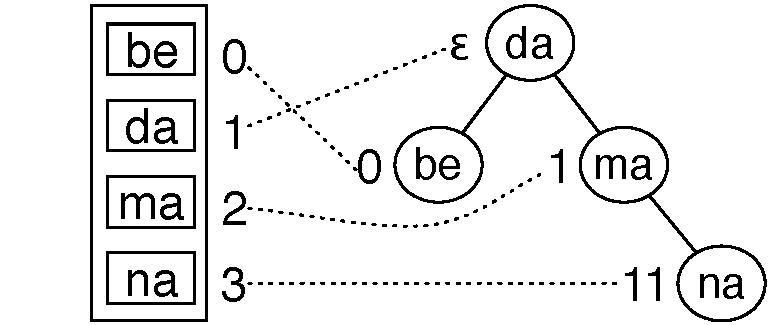
\includegraphics[scale=.32]{images/restruct1.pdf}
\end{wrapfigure}
The lens $\ell\in I\lens I'$ does not know anything about the intended
application; it has a trivial complement $\Unit$ and
merely maintains the constraint that the list shape and the tree shape
have the same number of positions. It has some freedom how it
translates list edits; e.g., it might add and remove tree nodes at the
left.

\ifdissertation
    \begin{wrapfigure}{r}{2in}
    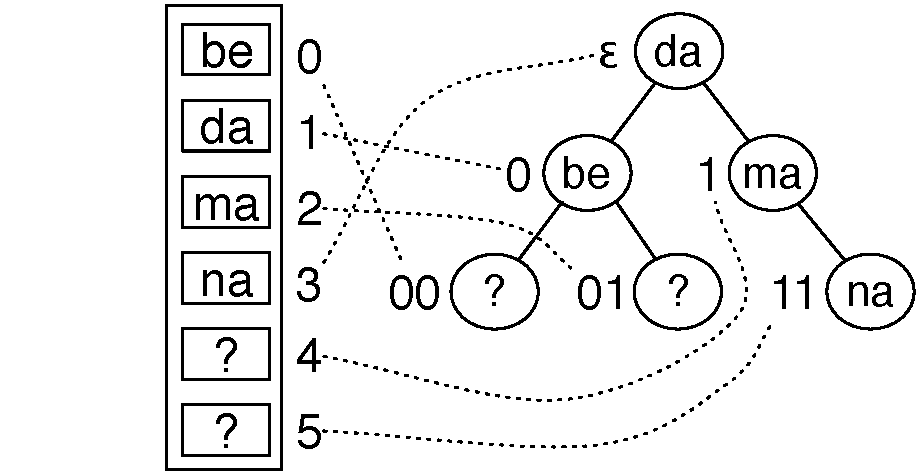
\includegraphics[scale=.32]{images/restruct2.pdf}
    \end{wrapfigure}
    The family of bijections $f_{i,c,i'}$ models the in-order correspondence;
\else
    The family of bijections $f_{i,c,i'}$ models the in-order
    \begin{wrapfigure}[9]{r}{1.3in}
    \hspace*{-4.3em}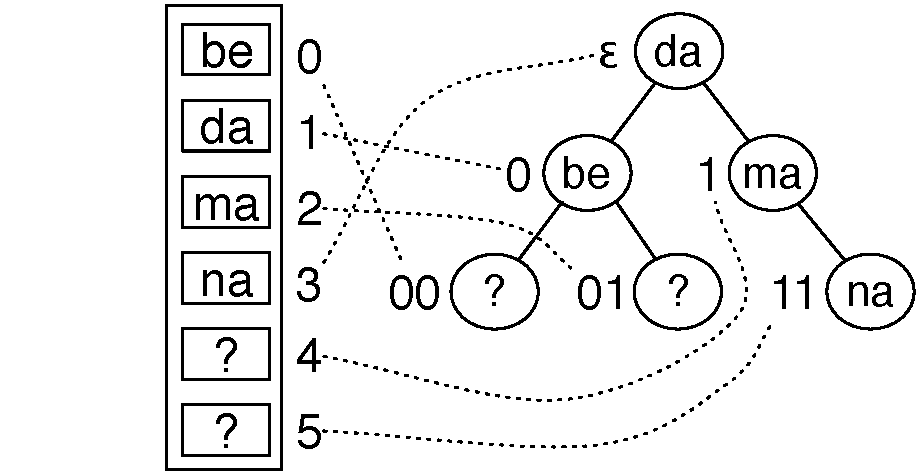
\includegraphics[scale=.32]{images/restruct2.pdf}
    \end{wrapfigure}
    correspondence;
\fi
thus, for example if $i=4$ and $i'=\{\NIL, \blist0\elist, \blist1\elist,
\blist1\mlist1\elist\}$ the bijection
would be as shown above. (For illustration we also indicate possible
$X$-contents of the positions.)
%
Formally, we have $f_{i,c,i'} = \{(0,\blist0\elist), (1,\NIL),
(2,\blist1\elist), (3,\blist1\mlist1\elist)\}$.

Now suppose that $\di\, i = i+2$ and that $\di'$ (the result of $\di$ propagated
through $\ell$) installs two children at the leftmost node. 
%
In our in-order application we then have $f_{\di\, i, c', \di'\, i'} =
\{(0,\blist0\mlist0\elist)$, $(1,\blist0\elist)$,
$(2,\blist0\mlist1\elist)$, $(3,\NIL)$, $(4,\blist1\elist)$,
$(5,\blist1\mlist1\elist)\}$ and
after applying both $\mlinsert(\di)$ and $\mlinsert(\di')$ we are in the
as-yet-inconsistent situation depicted above.
%% \begin{verbatim}
%% 0:be              eps:da
%% 1:da            /       \
%% 2:ma           0:be     1:ma
%% 3:na         /   \          \
%% 4:?        00:?  01:?        11:na
%% 5:?

%% Include the f-links, this time they go wild, eg 0 ----- 00 
%% \end{verbatim}

\ifdissertation\begin{wrapfigure}{r}{2in}
\else          \begin{wrapfigure}[9]{r}{1.3in}\hspace*{-4.3em}
\fi
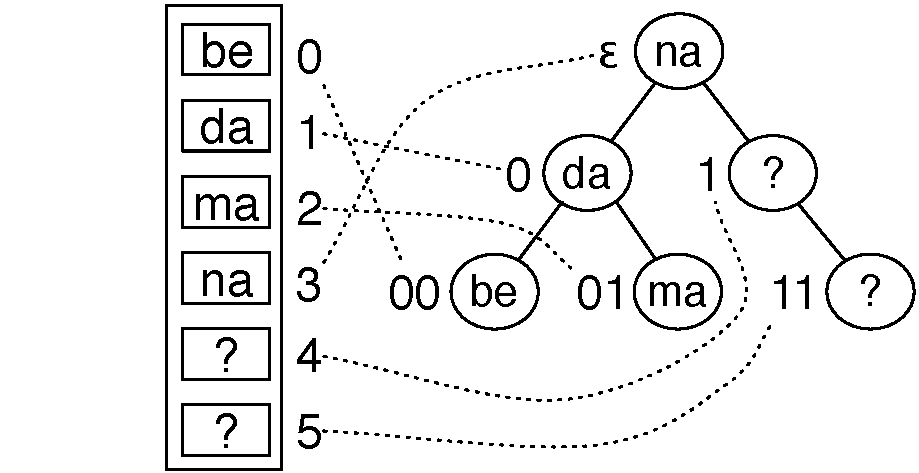
\includegraphics[scale=.32]{images/restruct3.pdf}
\end{wrapfigure}
Since the newly inserted elements in the list come at the end, we can
restore consistency by moving the newly inserted tree elements to positions
that come at the end of the in-order walk. This can be done essentially
automatically just using the in-order walk position bijections: to decide
where a position $p$ in the old tree should reappear in the new tree, we can
simply follow the position through its journey of being flattened and
unflattened using $f_{i,c,i'}$ and $f_{\di\;i,c',\di'\;i'}^{-1}$,
respectively. Thus to restore consistency we apply $\mlrearrange(\ONE,f_\mli)$ where
$f_\mli(i')=\{(\blist0\mlist0\elist,\blist0\elist)$, $(\blist0\elist,\NIL)$,
$(\blist0\mlist1\elist,\blist1\elist)$, $(\NIL,\blist1\mlist1\elist)$,
$(\blist1\elist,\blist0\mlist0\elist)$,
$(\blist1\mlist1\elist,\blist0\mlist1\elist)\}$. We could also have chosen
$f_\mli(i')= \{\dots, (\blist1\elist,\blist0\mlist1\elist)$,
$(\blist1\mlist1\elist,\blist0\mlist1\elist)\}$; since in any case the new
positions are uninitialized, this free choice has little impact.
Of course $f_\mli(i'')$ for $i''\neq i'$ is also
completely unconstrained. After applying $\mlrearrange(\ONE,f_\mli)$ we end up
with the desired consistent state.
%% \begin{verbatim}
%% 0:be              eps:na
%% 1:da            /       \
%% 2:ma          0:da     1:?
%% 3:na         /   \        \
%% 4:?        00:be  01:ma    11:?
%% 5:?
%% \end{verbatim}

\begin{figure}
% http://tex.stackexchange.com/q/121925/16779
\newtoggle{wide-equation}
\ifdissertation\settoggle{wide-equation}{true}\else\settoggle{wide-equation}{false}\fi
\newcommand{\wideeqbreak}{\iftoggle{wide-equation}{}{\\ &&}}
% \vspace*{-2.5ex}
\lensdef{w_restructuring}
{\infruleplain{T = \left<I,P,\live\right>\mbox{ a container type} \\
               T' = \left<I',P',\live'\right>\mbox{ a container type} \\
               \ell \in I \lens I'}
              {[T,T'](\ell) \in T(X) \lens T'(X)}}
 { C &=& \ell.K
  \\[.8ex]
  \missing &=& (\init_I,\ell.\missing,\init_{I'}) \\[.8ex]
  \colspan{K = \{ ((i,f),(i,c,i'),(i',f'))} \\
  \colspan{\qquad \;|\; (i,c,i')\in \ell.K \wedge \,\forall p{\in}\live'(i'). f(f_{i,c,i'}(p))=f'(p) \} } \\[1ex]
  \dputr\gen(\fail,x) &=& (\fail,x)\\
  \dputr\gen(\mlmod p\dx,(i,c,i')) &=& (\mlmod{f^{-1}_{i,c,i'}(p)}\dx, (i,c,i')) \\
  && \text{when }p\in\live(i)\\
  \dputr\gen(\mlinsert(\di),(i,c,i')) &=&
      (\mlrearrange(\ONE,f_\mli)\mlinsert(\di'), \wideeqbreak
      (\di\;i, c', \di'\;i'))\\
  \dputr\gen(\mldelete(\di),(i,c,i')) &=&
    (\mldelete(\di')\mlrearrange(\ONE,f_\mld), \wideeqbreak
    (\di\;i, c', \di'\;i'))\\
  \dputr\gen(\mlrearrange(\di,g),(i,c,i')) &=&
    (\mlrearrange(\di',f_\mlr), \wideeqbreak
    (\di\;i,c',\di'\;i'))\\[.8ex]
  && \text{see below for $f_\mli,f_\mld,f_\mlr$}\\
  \text{in the last three clauses:} && (\di',c')=\ell.\dputr(\di,c)\\
  \dputr\gen(\text{d}c,(i,c,i')) &=& \fail\text{ in all other cases}\\
  \dputl\gen(-,-) &=& \text{analogous}
  }
%
\makeatletter\refstepcounter{\@captype}\makeatother
\label{fig:restructuring-definition}
\vspace*{-3ex}
\begin{center}
{\bf Figure \ref{fig:restructuring-definition}:} Container restructuring lens
\end{center}
\vspace*{-3ex}
%  \caption{A lens for restructuring containers.}
\end{figure}

With this intuition in hand, we are ready to see the details of the
restructuring lens. As discussed above, we must have containers $T$ and
$T'$, an edit lens $\ell$ between their shapes, and a family of bijections
between live sets. We also require that $\ell$ maps insertions to
insertions, deletions to deletions, and rearrangements to rearrangements.
(This is well-defined on equivalence classes of lenses.)
Given these data, we define the restructuring lens in
Figure~\ref{fig:restructuring-definition}, with a few supplementary
definitions below.
%
The additional families of bijections $f_\mli, f_\mld, f_\mlr$ must be chosen in such a
way that the container edits in which they appear are well-formed
(this is possible since $\di'$ is an insertion, deletion, or
restructuring as appropriate) and such that the following three constraints are
satisfied: in each case $i,i'$, etc.,  refer to the current values from above and $p\in \live'(\di'\ i')$ is an arbitrary position. 
\begin{align*}
f_\mli(\di'\ i')(p) &=
\begin{array}[t]{@{}l}
f^{-1}_{i,c,i'}(f_{\di\ i,c',\di'\ i'}(p))\\ 
\quad \text{ when $f_{\di\ i,c',\di'\ i'}(p)\in\live(i)$}
\end{array}\\
f_\mld(i')(p) &= f^{-1}_{i,c,i'}(f_{\di\ i,c',\di'\ i'}(p))\\
f_\mlr(i')(p) &= f_{i,c,i'}^{-1}(g(i)(f_{\di\ i,c',\di'\ i'}(p)))
\end{align*}

These conditions do not completely determine $f_\mli$, $f_\mld$, and $f_\mlr$. In
each case, these families are completely unconstrained on shapes other than
$\di'\;i'$. The propagated edits are supposed to be applied to a container
of the current shape $i'$, so the arbitrary decisions about other shapes do
not really matter;
nevertheless it would be nice if we could be a bit more uniform. This
is indeed possible in the case where $\ell$ is an isomorphism lens, but we
refrain from formulating details.
% TODO: understand this sentence well enough to decide whether to formulate
% some details here-ish

As discussed in the example above, the bijection $f_\mli$ contains a little
more choice, namely the behavior on the $T'$ positions in $f_{\di\
i,c',\di'\ i'}^{-1}(\live(\di\ i)\setminus\live(i))$. Fortunately, they all
contain $\init_X$ so that the choice does not affect the resulting
state after application of the edit, and the alignment is decided not by
$f_\mli$ but by the family of bijections $f_{i,c',i'}$ that parameterize the
lens.

\iffull
\begin{theorem}
The restructuring lens is indeed a lens.
\end{theorem}
\begin{pf}
  As the edit monoid is free, we only need to show that successful
  edits to consistent states get transported to successful edits
  resulting in consistent states. Thus suppose that
  $(i,c,i')\in\ell.K$ and $f(f_{i,c,i'}(p))=f'(p)$ holds for all
  $p\in\live'(i')$ so that $((i,f),(i,c,i'),(i',f'))$ are consistent. We
  will show below that $\dputr$ is correct; the proof about $\dputl$ is very
  similar. In the cases below where there is an edit named $\di$, we will
  write $(\di',c')=\ell.\dputr(\di,c)$ and abbreviate the bijections
  $f_{i,c,i'}$ and $f_{\di\;i,c',\di'\;i'}$ to $f_{pre}$ and $f_{post}$,
  respectively.

  Case $\fail$ is obvious. 

  Case $\mlmod p\dx$: the complement does not change and the edit
  $\dx$ is applied to the same elements.

  Case $\mlins \di$. The resulting new repository states are $(\di\;i,f_1)$
  and $(\di'\;i', f_1')$:
  \begin{align*}
    f_1(p)&=\text{if }p\in\live(i)\text{ then }f(p)\text{ else }\init_X\\
    f_1'(p)&=\text{if }f_\mli(\di'\;i')(p)\in\live(i')\text{ then }f'(f_\mli(\di'\;i')(p))\text{ else }\init_X
  \end{align*}
Also, the bijection $f_\mli(\di'\ i')\in\live'(\di'\ i')\simeq \live'(\di'\ i')$ satisfies
\[
f_{post}(p)\in\live(i)\Rightarrow f_\mli(\di'\ i')(p)= f^{-1}_{pre}(f_{post}(p)).
\]
This assumption lets us conclude that $f_{post}(p) \in \live(i)$ if and only
if $f_\mli(\di'\;i')(p) \in \live'(i')$. In the forward direction, we argue:
\begin{align*}
    f_{post}(p) &\in \live(i) &&\mbox{assumption} \\
    f_{pre}^{-1}(f_{post}(p)) &\in \live'(i') &&f_{pre} \in \live(i) \simeq
    \live'(i') \\
    f_\mli(\di'\;i')(p) &\in \live'(i') &&\mbox{assumed condition of }f_\mli
\end{align*}
In the backward direction, define $q=f_\mli(\di'\;i')(p)$. Then:
\begin{align*}
    f_\mli(\di'\;i')(p) &\in \live'(i') &&\mbox{assumption} \\
    q &\in \live'(i') &&\mbox{definition of }q \\
    f_{pre}(q) &\in \live(i) &&f_{pre} \in \live(i) \simeq \live'(i') \\
    f_{post}(f_{post}^{-1}(f_{pre}(q))) &\in \live(i) &&f_{post}\mbox{ is a bijection} \\
    f_{pre}^{-1}(f_{post}(f_{post}^{-1}(f_{pre}(q)))) &= q
        &&f_{post}\mbox{ and }f_{pre}\mbox{ are bijections} \\
    f_\mli(\di'\;i')(f_{post}^{-1}(f_{pre}(q))) &= q
        &&\mbox{assumed condition of }f_\mli \\
    f_{post}^{-1}(f_{pre}(q)) &= p
        &&f_\mli(\di'\;i')\mbox{ is a bijection and} \\
       &&&\mbox{definition of }q \\
    f_{post}(p) &\in \live(i) &&f_{pre}(q)\in\live(i)
\end{align*}

To conclude the case, we must show that arbitrary $p \in \live'(\di'\;i')$
have $f_1'(p)=f_1(f_{post}(p))$. We consider two cases: either $f_{post}(p)
\in \live(i)$ or not. If so then $f_1(f_{post}(p))=$ $f(f_{post}(p)) = $
$f'(f_{pre}^{-1}(f_{post}(p)))= $ $f_1'(p)$ where the first equation uses
the above characterization of $f_1$; the second one uses consistency of $f$
and $f'$, and the third one uses the characterizations of $f_1'$ and $f_\mli$
(noting that $f_{post}(p) \in \live(i)$ implies $f_\mli(\di'\;i')(p) \in
\live'(i')$). In the other case, $f_{post}(p) \notin \live(i)$, so
$f_\mli(\di'\;i')(p) \notin \live'(i')$. Then $f_1'(p)=\init_X$, but
$f_1(f_{post}(p))=\init_X$, too, by the characterization of $f_1$.

  Case $\mldel \di$. Ignoring domain restrictions, the new repository states
  are $(\di\;i,f)$ and $(\di'\;i',f_\mld(i');f')$. For these to be consistent,
  we must show that $f(f_{post}(p)) = f'(f_\mld(i')(p))$ whenever $p \in
  \live'(\di'\;i')$. Since $\di$ is a deletion, we know $\di\;i \subset i$,
  so that $f_{post} \in \live(\di\;i) \simeq \live'(\di'\;i')$ implies
  $f_{post}(p) \in \live(i)$. Hence we can equate:
  \begin{align*}
      f(f_{post}(p)) &= f'(f_{pre}^{-1}(f_{post}(p)))
          &&\mbox{consistency of }f\mbox{ and }f'\\
      &= f'(f_\mld(i')(p)) &&\mbox{assumed condition of }f_\mld
  \end{align*}

  Case $\mlrearrange(\di,g)$. The new repository states that we must show
  are consistent are $(\di\;i,g(i);f)$ and $(\di'\;i',f_\mlr(i');f')$. Consider
  arbitrary $p \in \live'(\di'\;i')$. Since $f_{post};g(i) \in
  \live'(\di'\;i') \simeq \live(i)$, we know $g(i)(f_{post}(p)) \in
  \live(i)$; this justifies the first equation below.
    \begin{align*}
        f(g(i)(f_{post}(p))) &= f'(f_{pre}^{-1}(g(i)(f_{post}(p))))
            &&\mbox{consistency of }f\mbox{ and }f' \\
        &= f'(f_\mlr(i')(p))
            &&\mbox{condition of }f_\mlr
    \end{align*}
\vskip -1.8\baselineskip
\end{pf}
\fi

\iffull Using the container lens combinators, the
partition lens and
lens mediating between ``built-in'' lists and ``list containers'' we
can then plumb together a variety of useful lenses, e.g.\ one that
partitions the entries of an $X+Y$ labeled tree into $\inl$s and
$\inr$s and then presents the two resulting containers again as trees
over $X$ and $Y$. If one wants one can then use a mapping lens to
change the representation of the $Y$'s in some way.
\fi

\sect{Adding Monoid Laws}
\label{sec:monoid-laws}

The edit languages accompanying the constructions in the previous two
sections were all freely generated.  This was a good place to begin as it
is relatively easy to understand, but, as discussed in \S
\ref{sec:semantics}, there are good reasons for investigating richer
languages.  This section takes a first step in this direction by showing how
to equip the product and sum combinators with more interesting edits. 

Given modules $X$ and $Y$, there is a standard definition of {\em module
  product} 
motivated by the intuition that an edit to an $|X| \times |Y|$ value is a
pair of an edit to the $|X|$ part and an edit to the $|Y|$ part. The monoid
multiplication goes pointwise, and one can define an edit application that
goes pointwise as well.
\[
\begin{array}{@{}c@{}}
X \otimes Y = \left<|X| \times |Y|,(\init_X,\init_Y),\partial X \otimes
\partial Y,\odot_{X \otimes Y}\right> \\[.6ex]
\ONE_{M \otimes N} = (\ONE_M,\ONE_N) \\[.6ex]
(m,n)\cdot_{M \otimes N}(m',n') = (m\,m', n\,n')\\[.6ex]
(\dx,\dy)\odot_{X \otimes Y}(x,y) = (\dx\,x,\dy\,y)
\end{array}
\]

\iffull
\begin{lemma}
    These definitions give rise to a module---that is, $\cdot_{M \otimes N}$
    is associative with identity $\ONE_{M \otimes N}$ and $\odot_{X \otimes Y}$
    satisfies the monoid action laws.
\end{lemma}
\begin{proof}
    To show that $\cdot_{M \otimes N}$ is associative, using the fact that
    $\cdot_M$ and $\cdot_N$ are associative:
    \begin{align*}
        v_1 \cdot (v_2 \cdot v_3)
            &= (m_1,n_1) \cdot ((m_2,n_2) \cdot (m_3,n_3)) \\
            &= (m_1,n_1) \cdot (m_2 \cdot m_3,n_2 \cdot n_3) \\
            &= (m_1\cdot(m_2 \cdot m_3),n_1\cdot(n_2 \cdot n_3)) \\
            &= ((m_1 \cdot m_2) \cdot m_3,(n_1 \cdot n_2) \cdot n_3) \\
            &= (m_1 \cdot m_2, n_1 \cdot n_2)\cdot(m_3,n_3) \\
            &= ((m_1,n_1) \cdot (m_2,n_2)) \cdot (m_3,n_3) \\
            &= (v_1 \cdot v_2) \cdot v_3
    \end{align*}
    To show that $\ONE_{M \otimes N}$ is an identity for $\cdot_{M \otimes
    N}$, assuming $\ONE_M$ and $\ONE_N$ are the respective identities for
    $\cdot_M$ and $\cdot_N$:
    \begin{align*}
        (\ONE,\ONE)\cdot(m,n)
            &= (\ONE \cdot m,\ONE \cdot n) \\
            &= (m,n) \\
            &= (m \cdot \ONE,n \cdot \ONE) \\
            &= (m,n) \cdot (\ONE, \ONE)
    \end{align*}
    To show the monoid action laws are satisfied by $\odot_{M \otimes N}$,
    assuming these laws are satisfied by $\odot_M$ and $\odot_N$:
    \begin{align*}
        (\ONE,\ONE) \odot (x,y)
            &= (\ONE \odot x, \ONE \odot y) \\
            &= (x,y) \\
        ((m,n)\cdot(m',n'))\odot(x,y)
            &= (m \cdot m',n \cdot n')\odot(x,y) \\
            &= ((m \cdot m') \odot x,(n \cdot n') \odot y) \\
            &= (m \odot m' \odot x,n \odot n' \odot y) \\
            &= (m,n) \odot (m' \odot x,n' \odot y) \\
            &= (m,n) \odot (m',n') \odot (x,y)
    \end{align*}
\end{proof}
\fi

One might wonder whether the standard definition has any connection to the
definition we give earlier. One way to bridge the gap is to add equational
laws to the free monoid\footnote{To make this formal, treat the
equations as a relation between words in the free monoid; take the
reflexive, symmetric, transitive, congruence closure of this relation; and
quotient by the resulting equivalence relation.}. The equations below demand
that $\ml{left}$ and $\ml{right}$ be monoid homomorphisms, and that they
commute:
\begin{align*}
    \blist\mlleft\ONE\elist &= \NIL \\
    \blist\mlleft\dx\mlist\mlleft{\dx'}\elist &= \blist\mlleft{\dx\dx'}\elist \\
    \blist\mlright\ONE\elist &= \NIL \\
    \blist\mlright\dy\mlist\mlright{\dy'}\elist &= \blist\mlright{\dy\dy'}\elist \\
    \blist\mlleft\dx\mlist\mlright\dy\elist &= \blist\mlright\dy\mlist\mlleft\dx\elist
\end{align*}
It is not hard to show that the free monoid subject to the above
equations is isomorphic to the natural monoid product.

However, it is not obvious that the definitions relying on the free monoid
product remain well defined after imposing the above equations. In
particular, we must check that any monoid homomorphisms we defined respect
these laws. For homomorphisms $f$ specified via specification
of $f\gen$, it is enough to prove that, for each equational law $g=g'$, the
specification respects the law---i.e., $f(g)=f(g')$.

For example, to check that we can create a well-defined tensor product
module that includes the above equations, we must show that $\odot\gen$
respects the equations. For the commutativity equation, we must show 
\[\mlleft\dx\odot\gen\mlright\dy\odot\gen(x,y) =
\mlright\dy\odot\gen\mlleft\dx\odot\gen(x,y).\]
Simple calculation shows that both sides are equal to $(\dx\;x,\dy\;y)$, so
this law is respected; the rest follow similar lines.

Most importantly, we must check that the $\dputr$ and $\dputl$ functions are
still monoid homomorphisms; indeed, this check
makes these equations interesting as a {\em specification}: 
in addition to the usual round-tripping laws we expect of
state-based lenses, each non-trivial equation in a monoid presentation
represents a behavioral limitation on lenses operating on that monoid.
Take again the commutativity law:
\[\mlleft\dx\;\mlright\dy = \mlright\dy\;\mlleft\dx\]
The force of this law is that lenses operating on a monoid including this
equation must ignore the interleaving of $\ml{left}$ and $\ml{right}$ edits:
those two edits are treated independently by the lens.

\begin{lemma}
    Suppose $k$ and $\ell$ are lenses. For each of the equations above, if
    that equation is in force in the modules on both sides of the
    $k\otimes\ell$ lens, then the $\dputr$ and $\dputl$ functions defined
    above for this lens respect that equation.
\end{lemma}
\begin{proof}
We will show that $\dputr$ treats $\ml{left}$ as a monoid homomorphism and
lets $\ml{left}$ and $\ml{right}$ commute; the proofs that $\dputr$ treats
$\ml{right}$ as a monoid homomorphism and that $\dputl\gen$ respects all these
laws are similar.

To show that $\dputr$ respects the law $\blist\mlleft\ONE\elist=\NIL$:
\begin{align}
    \dputr(\blist\mlleft\ONE\elist,(c_k,c_\ell))
        ={}& \mllet (\dz,c_k')=k.\dputr(\ONE,c_k)\mline \nonumber\\
           & (\blist\mlleft\dz\elist,(c_k',c_\ell)) \nonumber\\
        ={}& (\blist\mlleft\ONE\elist,(c_k,c_\ell)) \label{eq:klens} \\
        ={}& (\NIL,(c_k,c_\ell)) \label{eq:law} \\
        ={}& \dputr(\NIL,(c_k,c_\ell)) \label{eq:one2}
\end{align}
Equation~\ref{eq:klens} follows because $k$ is a lens and hence $k.\dputr$
is a stateful monoid homomorphism. Equation~\ref{eq:law} follows by
assumption, and equation~\ref{eq:one2} follows by definition of $\dputr$.

Next we will show that $\dputr$ respects the law
$\blist\mlleft\dx\mlist\mlleft{\dx'}\elist=\blist\mlleft{\dx\dx'}\elist$. It
will be convenient to name a few things. Pick a state $c_k$ and define:
\begin{align*}
    (\dy',c_k') &= k.\dputr(\dx',c_k) \\
    (\dy,c_k'') &= k.\dputr(\dx,c_k')
\end{align*}
Since $k$ is a lens and hence in particular $k.\dputr$ is a stateful monoid
homomorphism, we can conclude that:
\[k.\dputr(\dx\dx',c_k)=(\dy\dy',c_k'')\]
We may now compute:
\[\begin{array}{l}
    \dputr(\blist\mlleft\dx\mlist\mlleft{\dx'}\elist,(c_k,c_\ell)) \\
    \qquad=
        \mllet (\dy',(c_k',c_\ell')) = \dputr\gen(\mlleft{\dx'},(c_k,c_\ell)) \mline \\
    \qquad{\phantom{={}}}
        \mllet (\dy'',(c_k'',c_\ell'')) = \dputr\gen(\mlleft\dx,(c_k',c_\ell')) \mline \\
    \qquad{\phantom{={}}}
        (\blist\dy''\mlist\dy'\elist,(c_k'',c_\ell'')) \\
    \qquad=
        \mllet (\dy'',(c_k'',c_\ell'')) = \dputr\gen(\mlleft\dx,(c_k',c_\ell)) \mline \\
    \qquad{\phantom{={}}}
        (\blist\dy''\mlist\mlleft{\dy'}\elist,(c_k'',c_\ell'')) \\
    \qquad=
        (\blist\mlleft\dy\mlist\mlleft{\dy'}\elist,(c_k'',c_\ell)) \\
    \qquad=
        (\blist\mlleft{\dy\dy'}\elist,(c_k'',c_\ell)) \\
    \qquad=
        \dputr\gen(\mlleft{\dx\dx'},(c_k,c_\ell)) \\
    \qquad=
        \dputr(\blist\mlleft{\dx\dx'}\elist,(c_k,c_\ell))
\end{array}\]

\ifdissertation
The final equation to preserve is
\else
Finally, we show that $\dputr$ respects the law
\fi
$\blist\mlleft\dx\mlist\mlright\dy\elist=\blist\mlright\dy\mlist\mlleft\dx\elist$.
As before, we choose a $c_k$ and $c_\ell$ and name a few intermediate
computations:
\begin{align*}
    (\dx',c_k') &= k.\dputr(\dx,c_k) \\
    (\dy',c_\ell') &= \ell.\dputr(\dy,c_\ell)
\end{align*}
Now we may compute:
\[\begin{array}{l}
\dputr(\blist\mlleft\dx\mlist\mlright\dy\elist,(c_k,c_\ell)) \\
    \qquad=
        \mllet (\dy',(c_k',c_\ell')) = \dputr\gen(\mlright\dy,(c_k,c_\ell)) \mline \\
    \qquad{\phantom{={}}}
        \mllet (\dx',(c_k'',c_\ell'')) = \dputr\gen(\mlleft\dx,(c_k',c_\ell')) \mline \\
    \qquad{\phantom{={}}}
        (\blist\dx'\mlist\dy'\elist,(c_k'',c_\ell'')) \\
    \qquad=
        \mllet (\dx',(c_k'',c_\ell'')) = \dputr\gen(\mlleft\dx,(c_k,c_\ell')) \mline \\
    \qquad{\phantom{={}}}
        (\blist\dx'\mlist\mlright{\dy'}\elist,(c_k'',c_\ell'')) \\
    \qquad=
        (\blist\mlleft{\dx'}\mlist\mlright{\dy'}\elist,(c_k',c_\ell')) \\
    \qquad=
        (\blist\mlright{\dy'}\mlist\mlleft{\dx'}\elist,(c_k',c_\ell')) \\
    \qquad=
        \dputr(\blist\mlright\dy\mlist\mlleft\dx\elist,(c_k,c_\ell))
\end{array}\]
The final line follows from the previous one by an argument almost identical
(but reversed) to the argument showing that the second-to-last line follows
from the first.
\end{proof}

Adding the first four equations lets us create a projection lens
out of smaller parts by observing that there are some new isomorphisms
available.
\iffull

\begin{defn}[Projection lenses]
\fi
Let $f$ and $g$ be the obvious isomorphisms connecting $X \otimes \Unit$ to
$X$ and $\Unit \otimes Y$ to $Y$.%
%
\iffull
\footnote{%
  \ifdissertation
  Unlike the analogous state-based lenses from Chapter~\ref{chap:complement},
  \else
  Readers familiar with earlier work on symmetric state-based
  lenses~\cite{HofmannPierceWagner10} may observe that, unlike the analogous
  state-based lenses,
  \fi these projections are \emph{not} parameterized by an
  element of the set that is being projected away. Never fear: this element
  is still available, as the $\init$ value of the appropriate module.
  }
\fi
%
\iffull
    \begin{align*}
        \pi_1 &= (\id_X \otimes \const_Y);\bij_f \\
        \pi_2 &= (\const_X \otimes \id_Y);\bij_g
    \end{align*}
\else
{} We can then define $\pi_1 = (\id_X \otimes \const_Y);\bij_f$ and $\pi_2 =
(\const_X \otimes \id_Y);\bij_g$. Thus, $\pi_1$ first throws away any
information in the right-hand part of a tuple with $\const_Y$, then
collapses the (now degenerate) tuple with $f$.
\fi
\iffull \end{defn} \fi

We conjecture that these additional laws introduce enough isomorphisms that
the tensor product gives rise to a symmetric monoidal category---that is,
that tuples may be reordered and reassociated freely, provided the lens
program acting on them is reordered and reassociated accordingly---but we
have not explored this possibility fully.

\iflater
\finish{To define a more useful diagonal in this setting, we could
  consider enriching the monoid structure with a $\mathit{merge}$
  operation...}
\fi

We can perform a similar process for sum edits. We add the following
equations:
\begin{align*}
    \blist\mlswitch_{jk}(m)\mlist\mlswitch_{ij}(m')\elist
        &= \blist\mlswitch_{ik}(m)\elist \\
    \blist\mlswitch_{ij}(m)\mlist\mlstay_i(m')\elist
        &= \blist\mlswitch_{ij}(m)\elist \\
    \blist\mlstay_j(m)\mlist\mlswitch_{ij}(m')\elist
        &= \blist\mlswitch_{ij}(mm')\elist \\
    \blist\mlstay_i(m)\mlist\mlstay_i(m')\elist
        &= \blist\mlstay_i(mm')\elist \\
    \blist d\mlist d'\elist
        &= \blist\fail\elist \qquad \mbox{in all other cases}
\end{align*}
This explains why we did not originally choose to have just two combinators,
$\mlswitch_L$ and $\mlswitch_R$, which would be interpreted as ``switch to
the left (respectively, right) side and reinitialize, no matter which side
we are currently on.'' The idea of the above equations is that they allow
us to collapse any sequence of edits down into a single one; if we only
allowed ourselves $\mlswitch_L$ and $\mlswitch_R$ forms, this would not be
possible. In particular, we need to represent the fact that a $\mlstay_L$
edit followed by a $\mlswitch_i$ edit fails when applied to a value tagged
with $\mlinrx$.

As with products, we must check that the remaining
definitions are well-formed.  \iffull\else In particular, it can be shown that,
in the module defined above for sums, $\odot\gen$ respects the above
equations, and that, if $k$ and $\ell$ are lenses, then
$(k\oplus\ell).\dputr\gen$ and $(k\oplus\ell).\dputl\gen$ respect the above
equations.  \fi

% TODO: \ml{inl} -> \mlinlx ?
\iffull
\begin{lemma}
    In the module defined above for sums, $\odot$ respects the above
    equations.
\end{lemma}
\begin{proof}
    We will give proofs for the first four equations with $i$, $j$, and $k$
    instantiated to $L$ (proofs for other instantiations are nearly
    identical). The final equation is respected because every pair of atomic
    edits not listed in the first four equations results in an edit that
    cannot be successfully applied to any value (just like the $\fail$ edit
    itself).

    For each of the four equations (instantiated to $L$ everywhere) $e=e'$,
    both $e\odot\mlinr y$ and $e'\odot\mlinr y$ are undefined, so we focus
    on $e\odot\mlinl x$ and $e'\odot\mlinl x$.

    \[\begin{array}{l}
        \blist\mlswitchll m\mlist\mlswitchll{m'}\elist \odot \mlinl x \\
        \qquad= \blist\mlswitchll m\elist\odot \mlinl{m'\odot \init} \\
        \qquad= \mlinl{m \odot \init} \\
        \qquad= \blist\mlswitchll{m}\elist \odot \mlinl x
    \end{array}\]

    \begin{align*}
        \blist\mlswitchll m\mlist\mlstayl{m'}\elist \odot \mlinl x
            &= \blist\mlswitchll m\elist \odot \mlinl{m'\odot x} \\
            &= \mlinl{m \odot \init} \\
            &= \blist\mlswitchll m\elist \odot \mlinl x
    \end{align*}

    \begin{align*}
        \blist\mlstayl m\mlist\mlswitchll{m'}\elist \odot \mlinl x
            &= \blist\mlstayl m\elist \odot \mlinl{m' \odot \init} \\
            &= \mlinl{m \odot m' \odot \init} \\
            &= \mlinl{mm' \odot \init} \\
            &= \blist\mlswitchll{mm'}\elist \odot \mlinl x
    \end{align*}

    \begin{align*}
        \blist\mlstayl m\mlist\mlstayl{m'}\elist \odot \mlinl x
            &= \blist\mlstayl m\elist \odot \mlinl{m' \odot x} \\
            &= \mlinl{m \odot m' \odot x} \\
            &= \mlinl{mm' \odot x} \\
            &= \blist\mlstayl{mm'}\elist \odot \mlinl x
    \end{align*}
\end{proof}

\begin{lemma}
    If $k$ and $\ell$ are lenses, then $(k\oplus\ell).\dputr\gen$ and
    $(k\oplus\ell).\dputl\gen$ respect the above equations.
\end{lemma}
\fi

\iffull
\begin{pf}
    We will show only that $\dputr\gen$ respects the equations; the argument
    for $\dputl\gen$ is similar.

    Choose arbitrary sum edits $e_1,e_2$ and initial complement $c_0 \in C$
    and define:
\iffull
    \begin{align*}
        e_{12} &= e_2e_1 \\
        (f_1,c_1) &= \dputr(e_1,c_0) \\
        (f_2,c_2) &= \dputr(e_2,c_1) \\
        (f_{12},c_{12}) &= \dputr(e_2e_1,c_0)
    \end{align*}
\else
$e_{12} = e_2e_1$; 
$(f_1,c_1) = \dputr(e_1,c_0)$;
$(f_2,c_2) = \dputr(e_2,c_1)$; and
$(f_{12},c_{12}) = \dputr(e_2e_1,c_0)$.
\fi
    We must show that $f_{12}=f_2f_1$ and $c_{12}=c_2$. We will go by case
    analysis on $e_1$ and $e_2$; however we can first rule out a few broad
    categories of such cases.
    \iffull
    When
    $\dputr(e_1,c)=(\fail,\mlfailed)$ fails, there is very little to prove;
    we know that $\dputr(e_2,\mlfailed)=(f_2,\mlfailed)$ for some $f_2$, and
    hence that $f_2f_1=\fail$. Furthermore, it is not hard to see by
    inspecting the cases where $\dputr(e_1,c)$ fails that $\dputr(e_{12},c)$
    will also fail for any $e_2$. Hence $f_{12}=\fail=f_2f_1$ and
    $c_{12}=\mlfailed=c_2$. Similarly, when $e_2$ results in a failure, any
    combined edit $e_{12}$ will also result in failure.  As a final broad
    category, when the lens has already failed (that is, when
    $c_0=\mlfailed$), we observe that the lens preserves the ``constructor''
    of the edit. Since the monoid multiplication inspects only the
    constructor, the required equation $f_2f_1=f_{12}$ will hold, and we
    will have $c_{12}=\mlfailed=c_2$.
    \else
    When the lens fails, the complement gets ``stuck'' in the
    $\mlfailed$ state, reducing the problem to checking only the monoid
    part of the function. Since $\fail\,e=e\,\fail=\fail$ these
    equations are easy to check\iflater; the full version of the paper details this\fi.
    \fi

    In the following, we therefore assume that no failure occurs.
    A few definitions will be convenient: \finish{the $s$ definition could
    have been used in the definition of the lens.} 
\[
\begin{array}{c}
        s(L,\dx) = k.\dputr(\dx,k.\missing) \qquad
        s(R,\dx) = \ell.\dputr(\dx,\ell.\missing) \\[1ex]
        t(L,x) = \mlinl x \qquad 
        t(R,y) = \mlinr y \\[1ex]
        u(\mlinl x) = L \qquad
        u(\mlinr y) = R \qquad
        u(\mlfailed) = \mlfailed
\end{array}
\]
    \iffull
    The cases now proceed as follows:
    \else
    We show only one case to give the flavor of the argument. \iflater The full proof
    can be found in the technical report available online.\fi
    \fi
    \begin{trivlist} \item[] 

\nextcase{$e_1=\mlswitch_{hi}(\dx'),e_2=\mlswitch_{ij}(\dx)$} We have
            $e_2e_1=\mlswitch_{hj}(\dx)$. Since we consider only non-failing
            cases, we know $u(c_0)=h$---that is to say, the complement and the
            edit are consistent, and
            we are translating a ``sensible'' edit. We know two
            things: first, $f_1 = \mlswitch_{hi}(\dy')$ for some $\dy'$, and
            second, $u(c_1)=i$. From there, we can define
            $(\dy,c) = s(j,\dx)$, 
            so that
            $(f_2f_1,c_2) = (\mlswitch_{hj}(\dy),t(j,c))$.
            Moreover, simple calculation (again observing that $u(c_0)=h$
            and hence that $e_{12}$ is a sensible edit to apply, according
            to the complement) shows that also
            $(f_{12},c_{12}) = (\mlswitch_{hj}(\dy),t(j,c))$,
            which is equal to the previous tuple, as desired.

\iffull
\nextcase{$e_1=\mlstay_i(\dx),e_2=\mlswitch_{ij}(\dx')$} Since we know no
            failure occurs, we must have $u(c_0)=i$.
            Therefore, $e_2$ is a sensible edit to apply, and so
            \[\dputr(e_2,c_0) = (\mlswitch_{ij}(\dy'),t(j,c))\]
            where $(\dy',c)=s(j,\dx')$. Furthermore, $e_1$ is a sensible
            edit to apply, so we know $u(c_1)=i$, and hence that:
            \[(f_2,c_2) = (\mlswitch_{ij}(\dy'),t(j,c))\]
            Furthermore, since
            \[f_1 = \mlstay_i(\dy)\]
            for some $\dy$, we know $f_2f_1=f_2$. But since $e_{12}=e_2$,
            \begin{align*}
                (f_{12},c_{12}) &= \dputr(e_{12},c_0) \\
                &= \dputr(e_2,c_0) \\
                &= \dputr(e_2,c_1) \\
                &= (f_2,c_2) \\
                &= (f_2f_1,c_2)
            \end{align*}
            as desired.

\nextcase{$e_1=\mlswitch_{ij}(\dx'),e_2=\mlstay_j(\dx)$} Again, we observe
            that we must have $u(c_0)=i$. Therefore we simply appeal to the
            homomorphism laws
            for $k.\dputr$ (when $j=L$) or $\ell.\dputr$ (when $j=R$). For
            example, when $j=L$ and hence $c_0=\mlinl c$, we can define:
            \begin{align*}
                (\dy',c') &= k.\dputr(\dx',k.\missing) \\
                (\dy,c'') &= k.\dputr(\dx,c') \\
                (\dy'',c''') &= k.\dputr(\dx\dx',k.\missing)
            \end{align*}
            Then, by computation:
            \begin{align*}
                (f_1,c_1) &= (\mlswitch_{il}(\dy'),\mlinl{c'}) \\
                (f_2,c_2) &= (\mlstayl\dy,\mlinl{c''}) \\
                (f_{12},c_{12}) &= (\mlswitch_{il}(\dy''),\mlinl{c'''}) \\
                f_2f_1 &= \mlswitch_{il}(\dy\dy')
            \end{align*}
            Finally, appealing to $k.\dputr$'s homomorphism law, we conclude
            $\dy''=\dy\dy'$ and $c'''=c''$, and hence that
            $(f_2f_1,c_2)=(f_{12},c_{12})$.

\nextcase{$e_1=\mlstay_i(\dx'),e_2=\mlstay_i(\dx)$} Much like the
            previous case, since $u(c_0)=i$, we appeal directly to the
            homomorphism law for the underlying $\dputr$ operations; the
            only difference from the previous case is that we begin with a
            complement that may not be $k.\missing$ or $\ell.\missing$.
\fi
    \endofpf
    \end{trivlist}
\end{pf}
\fi

Unfortunately, the $\partition$ lens as given does {\em not} respect the
above equations.  It seems possible to enforce them by also imposing
equations on list edits that coalesce adjacent $\ml{reorder}$ operations. We
leave this to future work.

In a similar vein, we can impose equations on container edits---indeed, we
need them, since we would like lists to form a
special case of containers so that, possibly after
\emph{restructuring}, we can \emph{partition} and reassemble
containers, too. These equations would in particular allow us to
coalesce adjacent reorderings and to reorder insertions and
deletions with other edits so that insertions and deletions
always come first. This would also give rise to a compact normal
form of container edits. Again, we leave this to future work. 

\sect{From State-Based to Edit Lenses and Back} 
\label{stateb}

\ifcomplement
In \cite{HofmannPierceWagner10}, we introduced a
state-based framework for bidirectional transformations called
\emph{symmetric lenses}.  We refer to them here as \emph{state-based symmetric
  lenses}.
\fi
Recall from\symmlenses that a state-based symmetric lens $\ell$
between \emph{sets} $X$ and $Y$ comprises a set of complements $C$, a
distinguished element $\smissing \in C$, and two functions
\begin{eqnarray*}
    \putr &\in& X \times C \to Y \times C\\
    \putl &\in& Y \times C \to X \times C
\end{eqnarray*}
\ifdissertation
satisfying some round-tripping laws.
\else
satisfying the following round-tripping laws:
\infrule[PutRL]{\putr(x,c) = (y,c')}{\putl(y,c') = (x,c')}
\infrule[PutLR]{\putl(y,c) = (x,c')}{\putr(x,c') = (y,c')} 
Equivalence of state-based symmetric lenses is defined through the
existence of a simulating relation between the respective complement
sets that relates the $\smissing$ elements and is preserved by
$\putl,\putr$. A characterization in terms of ``dialogues'' is also given. 
%
State-based symmetric lenses modulo equivalence form a category (they
compose) and support a variety of constructions, in particular tensor
product, sum, lists, trees, and container types.

\fi
Now, for any set $X$ we have the monoid $O_X$ whose elements (edits)
are lists of overwriting elements of $X$ modulo the equality $xx=x$. An
action of $O_X$ on $X$ is defined by $\NIL x=x$ and $\blist x\mlist w\elist\;y=x$
where $x\in X, w\in X\LIST$. Note that this is well defined as
$x(xy)=x=xy$. If, in addition, we have a distinguished element $x\in
X$, we thus obtain a module denoted $X_x$ where $|X_x|=X$ and
$\init_X=x$ and $\DX_x = O_X$.

\iffull
We are now ready to give the definition of the lifting operation that turns
any symmetric, state-based lens between inhabited types into a symmetric
edit lens\footnote{The unique state-based lens between uninhabited types can
be lifted to the unique edit lens between degenerate modules.}.
\lensdef{editize}
{\infruleplain
    {\ell \in X \lens Y \qquad x \in X\\
     \ell.\putr(x,\ell.\smissing) = (y,c_0)
    }
    {\D_x\ell \in X_x \lens Y_y}
}
{
    C &=& \ell.C \\
    \missing &=& c_0 \\
    K &=& \{(x,c,y) \mid \ell.\putr(x,c)=(y,c)\} \\
    \dputr\gen &=& \ell.\putr \\
    \dputl\gen &=& \ell.\putl
}
\else
Let  $\ell$ be  a state-based symmetric lens between $X$
and $Y$ along with element $x\in X$. Defining
$(y,c_0)=\ell.\putr(x,\ell.\smissing)$,
we then construct a symmetric edit lens $\D_x \ell$ between the
modules $X_x$ and $Y_y$ 
as follows: 
(1) $(\D_x\ell).C = \ell.C$;
(2) $(\D_x\ell).\missing = c_0$;
(3) $(\D_x\ell).\dputr\gen = \ell.\putr$;
(4) $(\D_x\ell).\dputl\gen = \ell.\putl$; and
(5) $(\D_x\ell).K = \{(x,c,y) \mid \ell.\putr(x,c)=(y,c)\}$.
\fi
$\D_x \ell$ is a symmetric edit lens and the passage from $\ell$
to $\D_x \ell$ is compatible with the equivalences on symmetric
lenses and symmetric edit lenses. The equations for $\dputr$ and $\dputl$
are well-defined because the round-trip law for symmetric lenses guarantees
that putting the same value twice in a row results in the same output both
times (hence if edits will be coalesced in $X_x$, they will be translated to
edits that get coalesced in $Y_y$),
and the consistency relation is likewise preserved because the roundtrip
laws for symmetric lenses guarantee that any given $\putr$ or $\putl$
results in a ``stable state''.

\iffull
\begin{theorem}
    If $k$ and $\ell$ are state-based lenses and $k\equiv\ell$, then
    $\D_xk\equiv\D_x\ell$.
\end{theorem}

\begin{proof}
Suppose $S$ is a witness that $k\equiv\ell$. Then we define
$\D_xS$ as follows:
\[\D_xS = \{(x,c_k,c_\ell,y) \mid (c_k,c_\ell) \in S
\land x \in X \land y \in Y\}\]

Let us write $(y_k,c_{0k})=k.\putr(x,k.\smissing)$ and
$(y_\ell,c_{0\ell})=\ell.\putr(x,\ell.\smissing)$. Since
$(k.\smissing,\ell.\smissing)\in S$, we know $y_k=y_\ell$ and
$(c_{0k},c_{0\ell})\in S$. The former equality tells us that at least the
two lenses have the same type---that is, $Y_{y_k}=Y_{y_\ell}$ as
modules---while the latter inclusion lets us observe that
\[(\init_{X_x},(\D_xk).\missing,(\D_x\ell).\missing,\init_{Y_y})=(x,k.\smissing,\ell.\smissing,y)\in\D_xS\]
where we abbreviate $y_k$ and $y_\ell$ by the name $y$.

It remains to show that $\D_xS$ is preserved by $\dputr$ and
$\dputl$ (definedness is not in question since the modules in question have
no partial edits); these arguments are very similar, so we focus on the one for
$\dputr$. We have $x_0 \in X,y_0 \in Y,(c_k,c_\ell) \in S,\dx \in X_x$. We
must show that computing $\dputr$ with these values produces values that
form a tuple in $\D_xS$. We proceed by induction on $\dx$.

In case $\dx=\NIL$, we are done: after computing $\dputr$, we still
have $x_0$, $y_0$, $c_k$, and $c_\ell$. Otherwise, $\dx = x_1\CONS\dx'$ and
the induction hypothesis tells us that if the two equations
\begin{align*}
(\D_xk).\dputr(\dx',c_k)&=(\dy_k,c_k')\\
(\D_x\ell).\dputr(\dx',c_\ell)&=(\dy_\ell,c_\ell')
\end{align*}
hold then $(c_k',c_\ell') \in S$ and $\dy_k=\dy_\ell$. We can then conclude
that if $k.\putr(x_1,c_k')=(y_k,c_k'')$ and
$\ell.\putr(x_1,c_\ell')=(y_\ell,c_\ell'')$ then $y_k=y_\ell$ and
$(c_k'',c_\ell'') \in S$ because $S$ is a witness that $k \equiv \ell$.
We now compute with these definitions that
$(\D_xk).\dputr(\dx,c_k)=(y_k\CONS\dy_k,c_k'')$ and
$(\D_x\ell).\dputr(\dx,c_\ell)=(y_\ell\CONS\dy_\ell,c_\ell'')$. But we
have already seen that $y_k\CONS\dy_k=y_\ell\CONS\dy_\ell$ and $(c_k'',c_\ell'') \in
S$, so we are done.
\end{proof}
\fi

Let $X$ be a module. A \emph{differ} for $X$ is a binary operation
$\dif \in X\times X \rightarrow \partial X$ satisfying
$\dif(x,x')x=x'$ and $\dif(x,x)=\ONE$.
%
Thus, a differ finds, for given states $x,x'$, an edit operation $\dx$
such that $\dx\ x=x'$ and $\dx$ is ``reasonable'' at least in the sense that
if $x=x'$ then the produced edit is minimal, namely $\ONE$.  For example,
the module $X_x$ for set $X$ and $x\in X$ admits the \emph{canonical
  differ} given by $\dif(x,x')=x'$ if $x\neq x'$ and
$\dif(x,x)=\ONE$, otherwise.

Given an edit lens $\ell$ between modules $X$ and $Y$,
both equipped with differs, we define a symmetric lens $|\ell|$%
\iffull
. The passage $\ell\mapsto|\ell|$ is compatible with lens equivalence.
\lensdef{uneditize}
{\infruleplain{\ell \in X \lens Y}
              {|\ell|\mbox{ a symmetric lens between }|X|\mbox{ and }|Y|}
}
{
    C &=& |X| \times \ell.C \times |Y| \\
    \smissing &=& (\init_X,\ell.\missing,\init_Y) \\
    putr(x,(x_0,c,y_0)) &=& (\dy\;y_0,(x,c',\dy\;y_0)) \\
    && \mbox{where }(dy,c')=\ell.\dputr(\dif(x_0,x),c) \\
    putl(y,(x_0,c,y_0)) &&\mbox{analogous}
}
\else
\ between $|X|$ and $|Y|$ by
(1) $|\ell|.C = |X|\times \ell.C\times |Y|$;
(2) $|\ell|.\missing = (\init_X,\ell.\missing,\init_Y)$;
(3) $|\ell|.\putr(x,(x_0,c,y_0))= (\dy\ y_0,\, (x,
c',\dy\ y_0))$ where $(\dy,c')=\ell.\dputr(\dx,c)$ and $\dx=\dif(x_0,x)$;
and 
(4) an analogous definition of $|\ell|.\putl$
This defines a symmetric lens $|\ell|$ between $|X|$ and $|Y|$,
and the passage $\ell\mapsto|\ell|$ is compatible with lens
equivalence.
\fi
\begin{theorem}\label{eqchar}
  Let $X,Y$ be sets with distinguished elements $x$ and $y$ and equip
  the associated modules $X_x$ and $Y_y$ with their canonical differs.
 %
  The constructions $|-|$ and $\D_x$ then establish a
  one-to-one correspondence between equivalence classes of edit lenses
  between $X_x$ and $Y_y$, on the one hand, and state-based lenses
  between $X$ and $Y$ for which $x$ and $y$ are already consistent, on the other.
\end{theorem}

\iffull
\begin{pf}
Let $\ell$ be a state-based lens between sets $X$ and $Y$ 
and let $x\in X$, $y\in Y$ satisfy
 $\ell.\putr(x,\ell.\smissing)=(y,\ell.\smissing)$.
To show that $|\D_x\ell|\equiv \ell$ we use the
simulation $R=\{((x,c,y),c)\mid \ell.\putr(x,c)=(y,c)\}$.
%
Conversely, if $\ell\in X_x\lens Y_y$ then $\ell\equiv
\D_{\init_X}|\ell|$. To see this, we use the simulation
$S=\{(x,c,(x,c,y),y)\mid x\in X,y\in Y,c\in\ell.C\}$. We omit the verification
of both simulations.%
\end{pf}
\fi

The theorem's condition that $(x,\ell.\smissing,y)$ already be a consistent
triple may look strong at first, but one can simply take an arbitrary lens
and ``step'' it once by $x$ (producing a new lens whose $\smissing$
component is given by $\putr$) to produce a lens with essentially the same
behavior but a stable $\smissing$ component.
We conjecture that this ``isomorphism'' between state-based and certain edit
lenses is also compatible with various lens constructors, in particular tensor
product and sum.  

\iflater
\sect{Asymmetric Edit Lenses} 

\soon{Needs written.}
\fi

\ifdelta
\iffull
\sect{Modules vs.\ Categories}
\label{cats}
\iflater\discuss{Martin: anything else we should cite here, besides Diskin
  and Johnson?  
%% Maybe: 
%%      Diskin, Z. and Cadish, B. (1995) Algebraic graph-based approach to
%%      management of multidatabase systems. In Proceedings of The Second
%%      International Workshop on Next Generation Information Technologies
%%      and Systems (NGITS '95)
%%   and
%%      Piessens, F. and Steegmans, E. (1995) Categorical data specifications.
%%      Theory Appl. Categ. 1, 156-173.
}\fi{}It has been proposed 
\cite{Diskin-Delta11,Johnson11} that categories should be used for
the role played here by modules. The objects $\text{Ob}(\mathbf{C})$ of the
category $\mathbf{C}$ then play the role of states, and for any two states $x,y$ the
morphisms from $x$ to $y$ (elements of the homset $\mathbf{C}(x,y)$)
represent edits that send $x$ to $y$. Thus, every edit carries with it
a unique state to which it applies,
and we lose the possibility of applying a single edit to more than
one state---a possibility we have exploited in a number of our
constructions here.
% To do this formally, we employ the following
% equivalent but less common presentation of small categories
% (categories that have a set as opposed to a class of objects).

% \begin{defn}
% A small category is given by the following data: 
% \begin{itemize}
% \item  a class $|\CC|$ of objects; 
% \item a set $\text{Mor}(\CC)$ of morphisms, 
% \item  two functions $\text{dom},\text{cod}\in\text{Mor}(\CC)\rightarrow |\CC|$, 
% \item a function
% $\text{id}\in|\CC|\rightarrow \text{Mor}(\CC)$ 
% \item a {partial}
% function $\circ\in\text{Mor}(\CC)\times\text{Mor}(\CC)\rightarrow
% \text{Mor}(\CC)$, such that
% \item $g\circ f$ is defined iff $\text{dom}(g)=\text{cod}(f)$ and then 
%   $\text{dom}(g\circ f)=\text{dom}(f)$ and   $\text{cod}(g\circ f)=\text{cod}(g)$; 
% \item $\text{dom}(\text{id}_X)=X=\text{cod}(\text{id}_X)$; and
% \item the following equations hold whenever they make sense: $f\circ (g\circ h)=(f\circ g)\circ h$ and $f\circ \text{id}_X=f$ and $\text{id}_X\circ f=f$. 
% \end{itemize}
% \end{defn}

More precisely, a module $X$ induces a category $\mathbf{C}_X$
where $\text{Ob}(\mathbf{C}_X) = |X|$ and
$\mathbf{C}_X(x,y)=\{m\mid mx=y\}$.  
%
Conversely, given a category $\CC$, we can construct an associated module
$X:=\Mod(\CC)$ with $|X|=\text{Ob}(\CC)$ and $\partial X=\{(x,f,y)\mid
f\in\CC(x,y)\} /\mathord{\sim}\cup\{\fail\}$ where $\sim$ is the equivalence
relation that identifies all elements of the form
$(x,\text{id}_X,x)$. The monoid multiplication is given by composition
in $\CC$, sending ill-typed multiplications to the left- and
right-absorptive element $\fail$.
%
Note that this construction is well defined on equivalence classes. The
action on $|X|$ is given by $(y,\text{id}_y,y)x=x$, by $(x,f,y)x'=y$ when
$x=x'$, and is undefined in all other cases.  Under a suitable notion of
morphism these back-and-forth constructions induce an equivalence (we omit
it for lack of space). However, these constructions do not constitute an
isomorphism because a single edit $e\in \partial X$ induces a fan of edits
in $\partial \Mod(\mathbf{C}_X)$, namely $\{(x,e,y)\mid ex=y\}$.

\fi%full
\fi%delta

% Consider a category $\CC$ and, by going back and forth, form the
% category $\DD:=\text{Cat}(\text{Mod}(\CC))$. We have $|\CC|=|\DD|$ and
% $\text{Mor}(\DD)=\{ (f,x)\mid f\ x \text{ is defined}\}$. Now, an element
% $(f,x)$ of $\text{Mor}(\DD)$ is either $(\ONE,x)$ where $\ONE$ is the
% equivalence class of all identities or it is of the form $(f,x)$ where
% $f$ is not an identity and $\text{dom}(f)=x$. It is thus clear that
% $\text{Mor}(\DD)$ is in 1-1 correspondence with $\text{Mor}(\CC)$ and
% in fact $\CC$ and $\DD$ are isomorphic categories. 

% Conversely, if we start with a module $X$ and form
% $Y:=\text{Mod}(\text{Cat}(X))$ then we can define a module
% homomorphism from $Y$ to $X$ by sending $x$ to $x$ and $(f,x)$ to $e$
% if $f$ is the equivalence class comprising the identities and to $\dx$
% if $f=(\dx,x')$. Conversely, sending $(\dx,x)$ to $(\dx,x)$ yields a
% module homomorphism from $X$ to $Y$ inverse to the previous one thus
% establishing that $X$ and $Y$ are isomorphic modules.


% \finish{There is a bunch of possibly useful old text commented out at this
%   point in the file.}

%% \subsection*{Old text from section 3...}

%% We sometimes also consider \emph{partial} variants of monoids and
%% modules, where the multiplication and action are partial
%% functions and the laws are understood in the sense that if either side
%% is defined then so is the other and they are equal. So, for example, if
%% $x:=m_1(m_2a)$ is defined, then $m_1m_2$ and $y:=(m_1m_2)a$ must both
%% be defined and $x=y$.

%% \finish{add the definition of the other
%% kind of module homomorphism}
%% \begin{defn}
%%     Given modules $X$ and $Y$, a \emph{module homomorphism}\finish{choose a
%%  new term that doesn't conflict with our earlier definition} from $X$ to $Y$
%%  is a pair of functions $f_0:|X|\rightarrow |Y|$ and 
%%     $f_1:\partial X \times |X| \rightarrow \partial Y$ such that 

%%     \infax{f_0(\dx \cdot x)= f_1(\dx,x)\cdot f_0(x)}

%%     \infax{f_1(\ONE,x)=\ONE}

%%     \infax{f_1(\dx_1 \odot \dx_2,x) = f_1(\dx_1, \dx_2x) \odot f_1(\dx_2,x)}

%% \bcp{A bit of intuition for the third law would be helpful.}

%% \noindent
%%     We write\bcp{angle brackets?} $(f_0,f_1):X\rightarrow Y$ to mean that $(f_0,f_1)$ is a
%%     module homomorphism. Often, the $f_0$ component is clear from the
%%     context, and we refer to the homomorphism merely by its $f_1$
%%     component.
%%     \bcp{Moved the following sentence from below.  But I'm not sure I
%%     understand its precise sense: is this a restriction on which pairs of
%%     functions are homomorphisms, or on what homomorphism application means?
%%     Probably it doesn't matter, but maybe the text can be reworded so the
%%     reader doesn't wonder.}(In the case of partial modules, the function
%%     $f_1$ is defined only on those pairs $(\dx,x)$ where $\dx\ x$ is defined.)

%%     For any module $X$ we have the identity homomorphism $\text{id}_X$
%%     given by $\text{id}_{X0}(x)=x$ and $\text{id}_{X1}(\dx,x)=\dx$. 
%%     If $f:X\rightarrow Y$ and
%%     $g:Y\rightarrow Z$ are module homomorphisms, then their composition
%%     $h=g\circ f$ is the module homomorphism $h:X\rightarrow Z$ given
%%     by $h_0=g_0\circ f_0$ and
%%     $h_1(\dx,x)=g_1(f_1(\dx,x),f_1(\dx,x)x)$.

%%     It is easy to check that this is indeed a homomorphism and that
%%     composition is associative with identities being neutral, so 
%%     (possibly partial) modules form a category $\Mod$.
%% \end{defn}

%% \subsection*{More old text from section 3...}

%% Several authors
%% \cite{waterloo,johnson} have proposed (small) categories as an alternative
%% model for sets of states with update operations. 

%% In this particular application of categories the objects of the
%% category  represent the states or models to be updated
%% whereas the morphisms represent the edits. Thus
%% each edit $f$ operates precisely on one state, namely $\text{dom}(f)$,
%% and the result of applying the edit to that very state will be
%% $\text{cod}(f)$.  As in the case of modules editing is associative and
%% there are identity edits. 

%% If $X$ is a (possibly partial) module then we can construct a category
%% $\Cat(X)$ where $|\Cat(X)|=|X|$ and $\text{Mor}(\Cat(X))=\{(x,\dx)\mid
%% \dx\ x\text{ is defined}\}$. We put $\text{dom}(x,\dx)=x$ and
%% $\text{cod}(x,\dx)=\dx x$ and $(x',\dx')\circ (x,\dx) = (x,\dx'\dx)$
%% provided that $x'=\dx x$. Notice that in this case $\dx'\dx$ is
%% automatically defined. Of course, $\text{id}_x=(\ONE,x)$, and it is easy
%% to see that this indeed defines a category. 

%% This operation extends to a functor in the sense that if
%% $f:X\rightarrow Y$ is a module homomorphism then we obtain a functor
%% $\Cat(f):\Cat(X)\rightarrow \Cat(Y)$ by setting $\Cat(f)_0(x)=f_0(x)$
%% and $\Cat(f)_1(x,\dx)=(f_0(x),f_1(\dx,x))$.


%% \begin{theorem}
%% The categories $\Mod$ of partial modules and $\Cat$ are equivalent. 
%% \end{theorem}
%% \begin{itemize}
%% \item Note that the monoids $\partial X$ and $\partial\Mod(\Cat(X))$ are not isomorphic
%% \item Modules are better for size reasons $\dx$ may be smaller than a morphism because it does not contain the state as part of it. 
%% \item  At least in the total case, are closer to traditional algebraic structures and simpler. 
%% \item There have been presentations of categories as partial monoids before, but the identification of all identities is new and cleaner than previous such attempts. 
%% \end{itemize}


%% \sect{String Edit Lenses}

%% \discuss{Cut this section?  Turn it into an implementation section?  (It
%%   would be nice to be able to say something about an implementation,
%%   particularly if it's ready to be made available publically.)}

%% \finish{this section should really be about reminding the readers of the
%% regular expression types stuff, with a separate section about the
%% implementation for discussing heuristics and things}
%% \begin{itemize}
%%     \item some things missing:
%%         \begin{itemize}
%%             \item parsing
%%             \item pretty-printing
%%             \item computing/representing edits
%%         \end{itemize}
%%     \item parsing/pretty-printing: same approach as with non-edit
%%         string lenses
%%     \item computing/representing edits: domain-specific, and almost
%%         inevitably heuristic at least a little
%%     \item sample domain: editor with two panes (one for each file format)
%%     \item distinction between string edits and edits to the algebraic
%%         structures the represent
%%     \item attach to each lens a translator function which takes the
%%         last-known-good string and a string edit (known to take it to a
%%         next-known-good string) and returns a structured edit
%%     \item modeling string edits: sequences of $\ml{insert}(n,s)$ and
%%         $\mldelete(n_1,n_2)$, where $n$s should be understood as positions
%%         \emph{between} two characters in the string
%%     \item lots more details to work out here
%% \end{itemize}
\mlinjnoargs

\chapter{Prototype Library for Edit Lenses}
\label{chap:implementation}
\label{chap:impl}

\section{Introduction}
\label{sec:impl-intro}
Having developed the theory of lenses and instantiating the framework with a
syntax, we now give an exposition on preliminary efforts to instantiate the
syntax as a concrete program. Our work on a prototype has two main purposes.
% TODO: the wording of this first purpose needs some serious polish
The edit lens framework is predicated on a relatively abstract, algebraic
data model, whereas long-term data storage on computers typically employs a
fairly low-level model based on strings. When only the data is important,
these two realms are typically connected by defining a parser that processes
strings and produces a more structured representation, as well as a
formatter that produces a string representation of a given structure. For
edit lenses, however, not only the data is important; one also wants access
to the edits made to the data. So the primary goal is to investigate what
extensions are needed to describe the connection between edits to strings
and edits to structured data. A secondary goal is to validate that the
fundamental edit lens design is complete; producing a few example
transformations gives an opportunity for any unforeseen infelicities to rear
their head. In the pursuit of these goals, we discuss two artifacts: first,
a core library which closely models the edit lens theory given in
Chapter~\ref{chap:edits}; and second, a demonstration program that
synchronizes two simple, text-based databases according to a predetermined
lens. The latter task involves building a text-editing GUI, connecting the
lens to the GUI, and validating and extracting edits from user actions,
tasks that fall outside the realm of the existing edit lens theory.

We have chosen to implement our demo in Haskell, a language which encourages
high abstraction levels, supports rapid prototyping, and has good library
support. Because one of our primary goals was experimentation, we wanted to
retain a lightweight approach throughout; in particular we chose not to
begin with a mechanization of the theory in a dependently-typed language.
(In retrospect, while it still seems worthwhile to have avoided reproving
all of our results in Coq from an experimentation point of view, it is not
clear that avoiding dependent types entirely was beneficial. For example,
the way we used Haskell's typeclass mechanism to model modules would really
have benefited from dependent types, as we often found ourselves wishing for
the ability to define new types for different choices of $\init$ value.) We
also investigated extending Boomerang~\cite{Boomerang07}, an existing
asymmetric, state-based string lens implementation. Boomerang is very
complete, and consequently would have required many tangential coding
efforts; to avoid distractions, we chose to take a less feature-complete
route. However, we retained Boomerang's choice of string-based data model
since, as discussed above, this closely matches real-world scenarios.

Our primary challenge, which we will discuss in detail below, can be broadly
described as parsing. With edit lenses, there are always two domains of
discourse: the collection of repositories and the collection of edits.
Repositories store ordinary data, and the problem of connecting strings with
structured data is well-studied under the umbrella of parsing. (Turning
structured data into a string---often called serialization---is typically a
significantly simpler task.) However, standard parsing techniques---even
incremental techniques purportedly designed for making it easy to maintain a
correct parse tree in the presence of ongoing updates---do not adequately
describe the connection between string modifications and edits in the sense
described in Chapter~\ref{chap:delta}. One could avoid the situation
entirely by designing a structured editor. Historically, though, structured
editors have failed to take---perhaps because their strictures are too
confining for day-to-day editing tasks---so we chose to avoid this route. We
have proposed a few heuristics that seem to behave acceptably in a number of
standard cases; however, they are relatively special-purpose (tailored to
the file format under consideration here) and do not adequately reflect all
user actions as analogous edits. This seems like a promising area for future
efforts.

\section{Usage Example and Functionality}
\label{sec:impl-usage}
In order to ground the discussion, we give here a quick overview of the
capabilities of the program we have built. When started, the program
presents a GUI containing two text-editing panes in which the user can
freely type. The two texts in the panes are connected by a lens, so that
when the text in one pane has been suitably modified, the text in the other
pane spontaneously changes to maintain synchrony. The particular lens we
will demonstrate below is a variant of the lens in
Figure~\ref{fig:span-lenses}, but instead of connecting teachers, salaries,
and room assignments, we will connect composers, birth years, and birth
countries. In one repository, we will have a list of newline-terminated
records, where each record has a composer's name and birth year separated by
a comma. In the other, each record has a composer's name and birth country
separated by a semicolon. Figure~\ref{subfig:prototype-1} gives a pair of
example synchronized repositories entered into our program's text panes. In
the abstract notation of Chapter~\ref{chap:edits}, the lens connecting the
two panes might be written as $(\id\otimes\disconnect)\LIST$. The concrete
lens used here must include a bit more information---for example,
instructions to change the comma separating parts of the record into a
semicolon, or a check that dates consist of exactly four digits---but we
will skip discussing these surface syntax issues for now.

The remainder of Figure~\ref{fig:prototype-screenshots} demonstrates how the
text panes would evolve under a few plausible edits to the repositories.
Part~\subref{subfig:prototype-2} shows what happens when the user adds an
extra line to the text pane on the right. As the right-hand repository now
has an extra record for Mozart, the lens produces an insertion that adds a
record for Mozart to the repository on the left, using a default birth year.
Since the insertion is inferred by watching the typing commands performed by
the user, the alignment for insertions of this kind can be exact: even if
the user were to duplicate a record from elsewhere in the database, no
confusion would arise, and a new record would appear with default data in
the correct location in the other repository. Similarly, when the user
deletes a line---in this case, the record for Haydn---on the right, the
program maintains synchrony by deleting the record for Haydn from the left
pane, as shown in part~\subref{subfig:prototype-3}. The left pane may also
be edited by the user, as demonstrated in part~\subref{subfig:prototype-4},
where Haydn has been re-inserted into the repository on the left, resulting
in a computed insertion containing a default country on the right. In
addition to the wholesale insertion and deletion of records, the user may
modify parts of a single record, and the program will correctly maintain
alignment of the edited records. Part~\subref{subfig:prototype-5} shows that
modifications to data that appears in only one repository has no effect on
the other, while in part~\subref{subfig:prototype-6} the user has corrected
the name ``Hayn'' to ``Haydn'' in the right repository, and this is
correctly reflected as an update to the left repository without losing
Haydn's birth year. Because we have access to the actions performed by the
user, we need not guess about whether the old ``Hayn'' record should be
aligned with the new ``Haydn'' record in this case. On the other hand, there
are certainly edits where the user intention is still not entirely clear;
parts~\subref{subfig:prototype-7} and~\subref{subfig:prototype-8} show the
user constructing a new record on the right that contains bits and pieces of
several old records (by performing a deletion that crosses record
boundaries). As pictured, our heuristics choose to treat this as a deletion
of all the old records that contributed and the insertion of a completely
fresh record, so a default birth year is used for the new record in the left
repository.

This final example begins to hint at some of the oddities that can arise
when attempting to translate between edits to a serialized structure and
edits to the abstract structure, which we will discuss in
\S\ref{sec:parsing}.

% TODO: this reverse highlighting experiment turned out a little strange
% because of the document's white background; let's try more orthodox
% highlighting or a circle around the change or something like that instead
\begin{figure}
    \centering
    \protofig1{An initial pair of databases in two text editing panes.}
    \hfil
    \protofig2{Insertion on the right introduces some default data on the
    left.}
    \vspace{4ex}

    \protofig3{Deleting a row from either side is reflected to the other
    automatically.}
    \hfil
    \protofig4{A default country is used for the new row on the right.}
    \vspace{4ex}

    \protofig5{Correcting the country has no effect\ldots}
    \hfil
    \protofig6{\ldots but correcting the spelling of either name corrects
    both.}
    \vspace{4ex}

    \protofig7{More bizarre edits, like this deletion that spans
    records\ldots}
    \hfil
    \protofig8{\ldots reset the alignment, but only for the affected region.}
    \vspace{4ex}

    \caption{A demonstration use of the prototype, using the composers lens}
    \label{fig:prototype-screenshots}
\end{figure}

\section{Parsing and edits}
\label{sec:parsing}
% TODO: redo the outline from here out based on committee feedback
annotated code, may describe selected functions or maybe all functions (?)
\begin{enumerate}
    \item edits + edit application: the Module type class
    \item lenses, simple lenses, lens+module triples
    \item basic lenses + maybe a few combinators
    \item unparsing (needs more motivation and explanation, or less if you consider this as not being reusable code)
    \item parsing (needs more motivation and explanation, or less if you consider this as not being reusable code)
    \item connecting to a GUI + storing complements in ref cells
    \item a `bad' choice - modules are based on type classes instead of being records
\end{enumerate}

\section{Conclusion}
\label{sec:impl-conclusion}
\begin{enumerate}
    \item Message: this is an existing library and an associated GUI that extracts alignment information from user actions
    \item Message: the existence of a working library is an indication that nothing important was overlooked in the theoretical foundation
    \item Message: this library could be used for further studies of edit lenses beyond the scope of the current work
        \begin{enumerate}
            \item original purpose: convert a string edit into a tree edit (resulted in a hard problem)
            \item demonstrate usability of the syntax by generating some practical examples
            \item show a performance advantage
            \item demonstrate a practical application of lenses (we have a long list of ideas about this)
        \end{enumerate}
    \item Outcome: we need new techniques for some parts, but core library can be elegant
\end{enumerate}

\section{Full code}
\label{sec:impl-code}
perhaps appendix, or pointers to hosting, or an attachment to the dissertation, or some such thing


\chapter{Related Work}
\label{chap:related}

\section{Graph-based delta lenses}
\label{sec:delta}
% TODO: change "source" and "target" to "domain" and "codomain" everywhere
% below to maintain consistency -- and to make the names \mldom and \mlcod
% more obvious

There is a closely related line of work focused on designing edit-based
lenses which begins with much the same motivation our work
does~\cite{diskin2011asymmetric,Diskin-Delta11,hermann2011correctness}. They
arrive at a slightly different point in the design space compared to us,
with a primary difference being their treatment of edits. For them, edits
are typed---with edit type $x \dedge x'$ classifying edits that can be
applied to value $x$ and result in value $x'$---and edit application is
total. Before we investigate their definitions of asymmetric and symmetric
delta lens, let us review their model of edits in detail. We will begin with
a few standard definitions to put some notation in place. Whenever possible,
we will pun notation between graphs and categories; after all, a graph with
suitable extra structure \emph{is} a category.

\begin{definition}
    A \emph{graph} $G$ is a quadruple $\left<G_0,G_1,\mldom,\mlcod\right>$
    consisting of a set of nodes $G_0$, a set of edges $G_1$, and two
    functions $\mldom,\mlcod \in G_1 \to G_0$ giving the source and target
    of each edge. We will write $e:v \dedge v'$ as shorthand for the
    assertion that $e \in G_1$, that $\mldom(e)=v$, and that $\mlcod(e)=v'$.
    If the directionality of the edge is uninteresting, we will write $e:v
    \uedge v'$ to mean either $e: v \dedge v'$ or $e: v' \dedge v$.
\end{definition}

Below, we will use graphs to model edits: nodes of the graph will correspond
to repository states, and an edge $\dx : x \to x'$ will correspond to an
edit $\dx$ which, when applied to state $x$, results in state $x'$. As in
our development, it is natural to impose a little bit of structure on edges,
such as the existence of a ``do-nothing'' edit and the ability to combine
two edits into one. We introduce these restrictions separately so that we
may talk about lenses between edit models with only some of this structure.
We will also introduce a constraint that says that no matter which two
repository states you choose, there is some edit between them, which may be
an important practical consideration but does not seem to affect the theory
significantly one way or another. For the discussion of symmetric delta
lenses, we will also want to consider edits which can be ``undone''.

\begin{definition}
    A graph $G$ is \emph{reflexive} if it comes equipped with a function
    $\id_G \in G_0 \to G_1$ which chooses a distinguished self loop
    $\id_{G,v} : v \dedge v$ for each node $v$. By abuse of notation, we
    will write $\id_v$ instead of $\id_{G,v}$ when there can be no confusion
    about which graph is meant.
\end{definition}

\begin{definition}
    A graph $G$ is \emph{connected} if for each $v,v'\in G_0$ there exists
    an edge $e : v \dedge v'$.
\end{definition}

\begin{definition}
    A reflexive graph $G$ is \emph{involutive} if it comes equipped with a
    function $\swoop \in G_1 \to G_1$ which associates with each edge $e : v
    \dedge v'$ an opposing edge $e\swoop : v' \dedge v$. It is required to
    be an involution (so that $e\swoop\swoop = e$) and to respect the
    reflexive structure of the graph (so that $\id_v\swoop=\id_v$).
\end{definition}

Before we come to a discussion of the lens frameworks proposed in this line
of work, it is worth comparing our modules to their choice of edit model.
They essentially consider two models: their asymmetric lenses are based on a
connected category model of edits, and their symmetric lenses are based on a
connected involutive graph model of edits.

In both cases, there is an underlying graph, and in particular this means
that each edit must uniquely identify the state that it can be applied to
along with the state it produces. At least naively, this requirement seems
to be in conflict with our goal of representing edits with objects
significantly smaller than the repository states. Many of our edit modules
exploit the ability to reuse edits as modifications to many different
repository states. Nevertheless, totality of edit application is a nice
feature. One can view the two approaches as two extremes, with on one end
graphs with a single node representing all possible repository states and on
the other end graphs with many nodes where each node represents a single
repository state. There may be a middle ground in which graph nodes each
represent many possible repository states; the hope then would be that one
could keep the benefit of a total edit application function while reusing
single edits on many different states. For example, for list edits, one
might consider a graph with one node for each possible length of list. Then
one would have, for example, deletion edges $\mldelete : m \dedge n$ when
$m<n$; such an edge must store marginally more information than our edit
module did (the source and target length rather than a single number telling
their difference), but the set of repositories to which it applies is much
more clearly delimited. Attempting to recast the edit modules and lenses
proposed above in this light would be an interesting area for future work.

The connection between modules and edit graphs can be made precise as
follows. To pass from a module $X$ to a graph $\Gr(X)$, let $\Gr(X)_0=|X|$
be the set of nodes and $\Gr(X)_1=\{m : x \dedge y \mid mx=y\}$ be the set
of edges (so that $\mldom(m : x \dedge y)=x$ and $\mlcod(m : x \dedge y)=y$,
hence $(m : x \dedge y) : x \dedge y$). The graph can be made reflexive by
defining $\id_x = \ONE : x \dedge x$; if we further define the composition
$(m : x \dedge y);(m' : y \dedge z)=mm' : x \dedge z$, the monoid action
laws guarantee that we can regard the graph as a category. Now let us see
how to pass from a category $G$ to a module $\Mod(G)$. (An arbitrary
reflexive graph may be turned into a category: for the arrows between nodes
$v$ and $v'$, use the set of paths from $v$ to $v'$ that do not have any
$\id$ edges\footnote{Equivalently, the set of paths quotiented by the
smallest congruence relation containing the equation that ensures that $\id$
edges are the unit for composition: $\blist \id \elist = \NIL$.}; for the
composition, use path concatenation; and for the identities, use empty
paths.) Let the values $|\Mod(G)|=G_0$ be the set of nodes, and edits $\D
\Mod(G)=\{\fail\}\cup G_1/\sim_\id$ be the set of edges quotiented by the
relation that identifies identities adjoined with a fresh absorptive failing
edit $\fail$. We let the identity element of the monoid $\ONE=\id$ be the
element representing the identities of the objects in the category;
multiplication is composition when well-typed and $\fail$ otherwise. Edit
application of $\ONE$ does nothing ($\ONE\odot x=x$); of well-typed edges
chooses the codomain ($(f : x \dedge y)\odot x=y$); and in all other cases
is undefined. One may choose any object to play the role of $\init$ (so that
there are as many ways to turn a category into a module as there are objects
in the category). Passing from a category to a module and back results in an
isomorphic category (because the freshly-adjoined $\fail$ edit is not an
arrow between any pair of objects); however, passing from a module to a
category and back may produce a significantly more verbose edit language:
each edit $m$ in the source module induces a collection of edits $\{m : x
\dedge y \mid mx=y\}$ in the target module.

The involutive graph model of edits demands the existence of undo edits,
something we did not consider carefully in the edit lens framework above. A
suitable module-based analog of the typed involution would be to require
each module to include an untyped involution $\swoop$ such that
$(\dx\swoop\;\dx)\odot x=x$ whenever $\dx\odot x$ is defined. (Thus
$\dx\swoop\;\dx$ is a restricted identity: not necessarily equal to $\ONE$,
but behaves like it for some subset of the values being edited.) Many of the
modules and module combinators we have defined above can be equipped with
this structure. A notable few that cannot include edit operations which
actually delete information, such as the sum module's $\ml{switch}$ edits
and the list module's $\mldelete$ edits. These edits would need to be
enriched or restricted to include the information being deleted; for
example, one could modify the action associated with $\mldelete$ edits to
only succeed when the list elements being deleted were $\init$ (so that
edits which wish to delete an element must first modify it to being $\init$
with $\mlmodify$ edits), and one could enrich the $\ml{switch}$ edits with
an edit that returns the value to a tagged $\init$ before switching sides of
the sum. Thus in general it seems that requiring an ``undo'' ability can
require mildly larger edit operations.

With these considerations about edits in mind, let us discuss how to
generalize asymmetric, state-based lenses first to asymmetric delta lenses
and then to symmetric delta lenses.

\subsection{Asymmetric}
\label{sec:delta:asymmetric}
Now, let us take the edit model above and see how to enrich asymmetric
lenses to take edit information rather than states. As with the state-based
version, we will assume that there is strictly more information in the
source category $S$ than in the view category $V$. This means that in the
\GET direction, it seems natural to assume that each source edit $\ds : s
\dedge s'$ uniquely determines a view edit $\dv : v \dedge v'$ by ``throwing
away'' the extra information. It is also quite natural to require this \GET
transformation to respect the category structure in $S$: that is, we should
expect $\aget(\id)=\id$ and $\aget(\ds;\ds')=\aget(\ds);\aget(\ds')$.
Together, these say that $\aget$ is a functor from $S$ to $V$.

As always, the \PUT direction is a bit more delicate because it needs to
restore missing information. Suppose we have a view edit $\dv : v \dedge
v'$ and wish to produce a source edit. It seems natural to wish that the
source edit we produce respects typing in the sense that if we produce $\ds
: s \dedge s'$, then $s$ is in the preimage of $v$ and $s'$ is in the
preimage of $v'$. But this is still very unconstrained; in particular, since
there really is a particular $s_0$ which is currently in synch with $v$, we
really want to produce an edit $\ds$ whose source is $s_0$---that is, there
is simply not enough information available in a view edit to produce a
reasonable translation function \PUT. So we cannot translate directly from a
view edit to a source edit; however, the key insight of this line of work is
that we can translate from a view edit to a \emph{family} of source edits
indexed by the source that is currently synchronized with the view.

In detail, given a functor $\aget \in S \to V$, we can construct the
preimage category $S/\aget$ as follows. The objects of $S/\aget$ are the
objects of $V$. The arrows $f : v \dedge v'$ of $S/\aget$ are the functions
which take a preimage $s$ of $v$ (i.e. such that $\aget(s)=v$) and produce
an arrow $f(s) : s \dedge s'$ of $S$ to a preimage $s'$ of $v'$ (i.e. such that
$\aget(s')=v'$). The identity arrow is the one which associates to each $s$
the arrow $\id_s$; the composition is defined by
$(f;g)(s)=f(s);g(\mlcod(f(s)))$. With this category in hand, we are ready to
define asymmetric delta lenses.

\begin{definition}
    An asymmetric delta lens $\ell \in S \adlens V$ between categories $S$
    and $V$ is a pair $\left<\aget,\aput\right>$ of functors $\aget \in S
    \to V$ and $\aput \in V \to S/\aget$ that satisfy the behavioral law:
    \infax[ADPutGet]{\aget(\aput(\dv)(s))=\dv}
\end{definition}

The suggested behavioral law enforces the intuition given above that all of
the information available in the view edits is available in source edits,
too. It turns out that the obvious definitions for identity and composition
lenses satisfy the behavioral law and induce a category whose objects are
categories and arrows are asymmetric delta lenses. As in our discussion
above relating edit lenses to symmetric lenses, one can connect asymmetric
delta lenses to asymmetric state-based lenses by adjoining an operation to
compute the difference between two states. The paper goes on to show that
asymmetric delta lenses only violate the controversial \rn{PutPut} law if
their differencing operation violates a similar \rn{DiffDiff} law---that is,
failure is never due to incorrect edit propagation, only incorrect edit
discovery.

One can construct an edit lens out of an asymmetric delta lens as follows.
The complement set will be source objects adjoined with a fresh $\fail$
value, so that the partial edit application can be extended to a total one
with explicit failure:
\begin{align*}
    \ds \odot_t \mlinl s &= \mlinl {\ds \odot s} & \ds\odot s\Defined \\
    \ds \odot_t s &= \fail & \mbox{otherwise}
\end{align*}
Then the lens construction goes as follows.
\lensdef{delta_symmetrize}
    {\infruleplain
        {\ell \in S \adlens V \quad s \in S_0}
        {\mlsymm_s(\ell) \in \Mod(S) \dlens \Mod(V)}
    }
    {
        C &=& S_0 \uplus \{\fail\} \\
        \missing &=& \mlinl s \\
        K &=& \{(s,\mlinl s,\ell.\aget_0(s)) \mid s \in S_0\} \\
        \dputr(\ds, s) &=& (\ell.\aget_1(\ds),\ds\odot_t s) \\
        \dputl(\dv, \mlinl s) &=& \mllet \ds = \ell.\aput_1(\dv)(s) \mlinm (\ds, \ds\odot_t s) \\
        && \mbox{when }\mldom(\dv)=\ell.\aget_0(s) \\
        \dputl(\dv, s) &=& (\fail,\mlinr \fail) \mbox{ otherwise}
    }
% TODO: prove this is well-defined (respects the equivalence class that \Mod
% introduces) and an edit lens
We conjecture that a construction similar to the one used to decompose
symmetric lenses into a pair of asymmetric, state-based lenses can be used
to decompose edit lenses into a pair of asymmetric delta lenses.
% TODO: could try to flesh out this conjecture a bit

The asymmetric delta lens framework described above is motivated by the
difficulty of alignment problems in the state-based lens world. It seems
plausible that an approach like this one could, indeed, address that
problem; however, no examples of lenses are given. This makes it difficult
to assess whether the behavioral laws are achievable or whether the
alignment problem is suitably addressed.

\subsection{Symmetric}
\label{sec:delta:symmetric}
Diskin et al. also spend some effort considering what machinery is needed to
support transformations between domains that each have missing
information---that is, symmetric transformations~\cite{Diskin-Delta11}. As
we observed in our symmetric lens development, passing from asymmetric to
symmetric lenses is cleanest if one introduces a complement---some extra
information about how the values in the two repositories correspond. This
development similarly allows for extra information, with a little bit of
extra notational complexity arising from the pervasive use of typing: edits
are typed via a category, as discussed above, and correspondence information
is also typed, as we discuss now.

% TODO: this might need more introduction

\begin{definition}
    Given graphs $G$ and $H$, we define the \emph{source-} and
    \emph{target-coincident} edge pairings as follows:
    \begin{align*}
        G \domco H &= \{(e_g,e_h) \mid e_g : v \dedge v' \in G_1 \land e_h :
        v \uedge v'' \in H_1\} \\
        G \codco H &= \{(e_g,e_h) \mid e_g : v \dedge v' \in G_1 \land e_h :
        v' \uedge v'' \in H_1\}
    \end{align*}
\end{definition}

\begin{definition}
    A \emph{symmetric delta lens} $\ell$ connecting model spaces $X$ and
    $Y$, written $\ell \in X \sdlens Y$, consists of:
    \begin{itemize}
        \item a bipartite graph $R$ whose two parts are $X_0$ and $Y_0$ (the
            edges of $R$ are called \emph{correspondence relations}),
        \item a function $\mlfppg \in X \domco R \to Y_1 \times R_1$,
            and
        \item a function $\mlbppg \in Y \domco R \to X_1 \times R_1$.
    \end{itemize}
    We will write $\mlfppg_1$ and $\mlfppg_2$ (and similarly for $\mlbppg$)
    for the $Y_1$ and $R$ parts of $\mlfppg$'s output, respectively.
\end{definition}

The preconditions for $\mlfppg$ above stating that the edit and
correspondence relations are source-coincident is somewhat similar to our
precondition requiring an edit which applies cleanly.

A major contribution of this line of research is an exploration of
behavioral guarantees that reasonable symmetric delta lenses might offer.
The obvious laws are too strong; but the insight of this development is that
if we take the obvious laws and replace equalities by a slightly coarser
equivalence relation, we get laws that are much more plausible. The core of
the problem is that equality on $X$ edits distinguishes between edits that
modify information not available in $Y$; we would prefer a relation that
compares only the parts of the edit that affect the shared information.
At first it seems difficult to define ``shared information'' formally, but
lenses are exactly transformations that define what information is shared;
so the relation is parameterized by a lens.

\begin{definition}
    Given function $f \in X \to Y$ we say $x$ and $x'$ are \emph{equivalent
    under $f$}, denoted $x \under_f x'$, when $f(x)=f(x')$.
\end{definition}

It is easy to see that $\under_f$ is an equivalence relation for any $f$.

\begin{definition}
    Given symmetric delta lens $\ell \in X \sdlens Y$ and a correspondence
    relation $r : x \uedge y$ for $\ell$, we define equivalence relations on
    edits to $x$ and $y$, respectively:
    \begin{align*}
        \eqsharedl*\ell r &={} \under_{\lambda \dx.\;\ell.\mlfppg_1(\dx,r)} \\
        \eqsharedr*\ell r &={} \under_{\lambda \dy.\;\ell.\mlbppg_1(\dy,r)}
    \end{align*}
    When the lens is understood from context, we will write $\dx\eqsharedl
    r\dx'$ instead of $\dx\eqsharedl*\ell r\dx'$ (and similarly for
    $\dy\eqsharedr r\dy'$).
\end{definition}

Armed with this notation, they propose several possible restrictions that
one could place on symmetric delta lenses. The first two restrictions are
analogous to ones discussed in our work above. Like our demand that
applicable edits get translated to applicable edits that restore
consistency, rule \rn{SDWellTyped} below demands that the edits and
correspondence relations involved in an invocation of $\mlfppg$ form a
well-typed square. They also demand that the propagation functions preserve
the self-loop structure of the edit graphs via the \rn{SDIdId} rule.
\infrule[SDWellTyped]
    {\mlfppg(\dx,r) = (\dy,r')}
    {r  : \mldom(\dx) \uedge \mldom(\dy) \\
     r' : \mlcod(\dx) \uedge \mlcod(\dy)}
\infrule[SDId]{r : x \uedge y}{\mlfppg(\id_x,r)=(\id_y,r)}

The edit graphs have another kind of structure given by the $\swoop$
undo operation. One might hope that this structure is preserved in a similar
way; for example, a rule like \rn{SDUndo-Strong*} seems reasonable at first
blush.
\infrule[SDUndo-Strong*]
    {\mlfppg(\dx,r)=(\dy,r')}
    {\mlfppg(\dx\swoop,r')=(\dy\swoop,r)}
Unfortunately, this rule is very restrictive. Suppose the $Y$ side of the
lens were to store some information not available in the $X$ side, and
propagating $\dx$ produces a $\dy$ that deletes some of that information.
Then this information could not be restored from the information in
$\dx\swoop$\footnote{One could imagine storing just enough information in
the correspondence relations to allow undoing one operation. Perhaps this
could be made to work, but it is unlikely this would scale well in
situations where there are composite edits (and hence composite undos).}.
One way to weaken this law to something more plausible would be to demand
that we output something that behaves like $\dy\swoop$ on the shared
information; that is, by weakening the equality in the conclusion to our
coarser equivalence relation from above:
\infrule[SDUndo]
    {\mlfppg(\dx,r)=(\dy,r')}
    {\mlfppg_1(\dx\swoop,r') \eqsharedr{r'} \dy\swoop}

The fourth and final behavioral law proposed demands that the edit
propagation functions be near inverses: that is, if we propagate $\dx$ to
$\dy$, then the corresponding edit determined by the other propagation
function should be $\dx$. As stated, this law is again too strong, because
some of the modifications described by $\dx$ are to unshared data, and hence
are not available in $\dy$ during re-propagation. As before, we can make the
rule more reasonable by weakening from equality to equivalence:
\infax[SDInvertible]{\mlbppg_1(\mlfppg_1(\dx,r),r)\eqsharedl r\dx}
This behavioral law is called a roundtrip law in their development, but that
name is a little misleading, as the update to the $y$ value and the updated
correspondence relation are discarded before applying the $\mlbppg$
function. (It is as if two separate people happened to take flights that
crossed paths in the middle, rather than a single person taking a round
trip.) We will instead call this law a \emph{triple-trip} law---for the two
trips evident in the law plus one trip hidden by the equivalence relation.

The line of research goes on to describe other theoretical
frameworks with interfaces closer to what an end-user programmer might want
to implement that can give rise to symmetric delta lenses. In particular,
they describe a framework they call \emph{consistency
maintainers}~\cite{Diskin-Delta11} which include explicit alignment and
consistency-restoration phases as well as explore conditions under which a
triple-graph grammar can be used to produce a law-abiding
lens~\cite{hermann2011correctness}. No concrete instantiations are given for
any of the three frameworks. We have found that undertaking this endeavor is
a valuable crucible in which to test prospective frameworks, as the design
of a lens language makes a mismatch between behavioral laws and actual
behavior much more clear. (Just as a good framework helps to spot
potential implementation bugs, an implementation helps point out potential
framework bugs.) In particular, sequential composition---in our experience,
a crucial tool for building practical lenses---is not considered, and the
ensuing need for a notion of lens equivalence is not addressed.

The proposed \rn{SDInvertible} and \rn{SDUndo} laws seem on the surface to
be quite natural restrictions. Our development does not have analagous laws,
and it seems that including them would necessitate a stronger equational
theory for many of the modules proposed above. Exploring the consequences of
these laws could be an interesting avenue for future work on edit lenses.

\section{Algebraic rephrasing}
\label{sec:algebraic}
% TODO: Do we need to mention somehow that this is a continuation of the
% (similarly-algebraically-motivated) exploration of state-based lenses in
% the 2007 Stevens paper that's cited elsewhere?
There is a line of work on algebraic foundations for delta lenses that
arrives at a model very similar to the edit lens framework described
above~\cite{stevens2008tat}. They consider, as we do, edit monoids together
with edit translation morphisms and (total) edit application actions.
One significant difference is that they consider generalizing asymmetric
rather than symmetric lenses, adopting correspondingly modified behavioral
laws. In particular, in their setting, a delta lens is a \emph{lens-like
split short exact sequence}. Below we discuss each of these restrictions in
right-to-left order. We begin with two standard definitions to establish
some notation.

\begin{definition}
    The \emph{image} of a function $f \in X \to Y$ is the set of elements
    $\im(f) \subset Y$ that $f$ can output:
    \[\im(f) = \{f(x) \mid x \in X\}\]
\end{definition}

\begin{definition}
    The \emph{kernel} of a monoid homomorphism $f$, denoted $\ker(f)$, is
    the preimage of $\ONE$:
    \[\ker(f) = \{x \mid f(x) = \ONE\}\]
\end{definition}

\begin{definition}
    An \emph{exact sequence} is a sequence $\blist f_1 \clist f_n \elist$ of
    monoid morphisms with compatible domains and codomains, that is,
    \begin{diagram}
        \path
            node                      (0)    {$X_0$}
            node[right=2.5em of 0]    (1)    {$X_1$}
            node[right=2.5em of 1]    (2)    {$X_2$}
            node[right=2.5em of 2]    (dots) {$\cdots$}
            node[right=2.5em of dots] (n2)   {$X_{n-2}$}
            node[right=2.5em of n2]   (n1)   {$X_{n-1}$}
            node[right=2.5em of n1]   (n0)   {$X_n$}
            (0)    edge[->] node[above] {$f_1$}     (1)
            (1)    edge[->] node[above] {$f_2$}     (2)
            (2)    edge[->] node[above] {$f_3$}     (dots)
            (dots) edge[->] node[above] {$f_{n-2}$} (n2)
            (n2)   edge[->] node[above] {$f_{n-2}$} (n1)
            (n1)   edge[->] node[above] {$f_n$}     (n0)
        ;
    \end{diagram}
    and such that $\im(f_i)=\ker(f_{i+1})$ for each $i$.
\end{definition}

\begin{definition}
    An exact sequence is \emph{short} if it has four morphisms and starts
    and ends at $\D\Unit$:
    \begin{diagram}
        \path
            node                   (1-1) {$\D\Unit$}
            node[right=4em of 1-1] (K)   {$K$}
            node[right=4em of K]   (X)   {$\DS$}
            node[right=4em of X]   (Y)   {$\DV$}
            node[right=4em of Y]   (1-2) {$\D\Unit$}
            (1-1) edge[->] node[above] {$i$} (K)
            (K)   edge[->] node[above] {$k$} (X)
            (X)   edge[->] node[above] {$f$} (Y)
            (Y)   edge[->] node[above] {$s$} (1-2)
            ;
    \end{diagram}
    We will say \emph{around} to mean the third element of a sequence, as
    in, ``$\blist i \mlist k \mlist f \mlist s \elist$ is a short exact
    sequence around $f$.''
\end{definition}

Before we define what split and lens-like mean, let us consider when an
edit translation homomorphism $f \in \DS \to \DV$ may be extended to a short
exact sequence. The homomorphism $s \in \DV \to \D\Unit$ must be the
constantly-$\ONE$ function (there are no other functions with that type), so
that its kernel is $\ker(s)=Y$. Hence the restriction $\im(f)=\ker(s)$ that
arises from extending the sequence to the right says that $f$ must be
surjective. On the other hand, the sequence may always be extended to the
left by choosing $K$ to be the submonoid $\ker(f)$ and $k$ to be the
inclusion function. (The homomorphism $i$ is completely determined by the
homomorphism laws once we have chosen a monoid $K$: it must map the sole
input element $\ONE_{\D\Unit}$ to $\ONE_K$.) Other choices for $K$ are
possible---for example, by adding a fresh generator to $K$ that $k$ maps to
any non-trivial element of $X$---but we will not be interested in this
ability below.

In lens terms, one should think of $f$ as being an edit-lens analog of the
asymmetric lens framework's \GET function. Giving a short exact sequence
amounts to identifying an edit translation function $f\in\DS\to\DV$ that is
compatible with the monoid structure on edits and such that each $V$-edit
has at least one analogous $S$-edit.

\begin{definition}
    A short exact sequence around $f\in\DS\to\DV$ is said to \emph{split} if
    there is a homomorphism $g\in\DV\to\DS$ such that $g;f = \id_{\DV}$.
\end{definition}

We are guaranteed that there is a \emph{function} $g$ by the fact that $f$
is surjective, but not guaranteed that any such function is a monoid
homomorphism. If we do have such a homomorphism $g$ that splits the
sequence, then in lens terms we should consider that $g$ to be an edit-lens
analog of the \PUT function. Then $g;f = \id_{\DV}$ says that all the
information available in $V$-edits are also available in $S$-edits, an
analogous restriction to the one on state-based lenses that says that all
the information available in the view repository is available in the source
repository.

The final condition placed on this variant of delta lenses is that they be
lens-like. Thus far, all the conditions have been purely in terms of edits;
this final pair of properties connect the world of edits and the world of
states. This is similar to the edit lens law that requires $\dputr$ and
$\dputl$ to respect a consistency relation on states.

\begin{definition}
    A monoid action $\odot \in \DX \times |X| \to |X|$ is \emph{transitive}
    if for all $x,x' \in |X|$ there is $\dx \in \DX$ such that $\dx\odot
    x=x'$. We will say a module is transitive when its action is.
\end{definition}

\begin{definition}
    A short exact sequence around $f\in\DS\to\DV$ split by $g$ is
    \emph{lens-like} if it comes equipped with transitive, total modules for
    $\DS$ and $\DV$ such that two conditions hold:
    \infrule[LL1]
        {\ds\;\init_S = \ds'\;\init_S}
        {f(\ds)\;\init_V = f(\ds')\;\init_V}
    \infrule[LL2]
        {\dv\;f(\ds)\;\init_V = f(\ds)\;\init_V}
        {g(\dv)\;\ds\;\init_S = \ds\;\init_S}
\end{definition}

Rule \rn{LL1} amounts to saying that $f$ is (part of) a module homomorphism
(not just a monoid homomorphism). Rule \rn{LL2} is a bit more subtle, but is
motivated by this rephrasing of the state-based asymmetric lens framework's
\rn{GetPut} law:
\infrule[GetPutAlt]
    {\aget(s)=v}
    {\aput(v,s)=s}
Rule \rn{GetPutAlt} says, roughly, ``if the view $v$ has not changed since
the last synchronization, then the source $s$ should not change, either.''
Similarly, \rn{LL2} says, roughly, ``if the edit we are about to translate
does not change the view $f(\ds)\;\init_V$, then the edit we output should
not change the source $\ds\;\init_S$.''

That work goes on to explore the properties of this kind of delta lens. One
can take a lens-like sequence around $f\in\DS\to\DV$ equipped with a diffing
operation $\dif\in|S|\times|V|\to\DV$ (satisfying the obvious sanity
condition) and produce an asymmetric, state-based lens. Additionally, there
is a close relationship between demanding the existence of inverse
edits---that is, working with edit groups rather than edit monoids---and the
\rn{PutPut} asymmetric lens law:
\infax[PutPut]{\aput(v,\aput(v',s))=\aput(v,s)}
They show that one can define suitably restricted submonoids $\DV \subset V
\to V$ and $\DS \subset S \to S$ and lift \rn{PutPut}-abiding asymmetric
lenses into a lens-like sequence on groups. Furthermore, the two
translations agree with each other: converting a lens to a lens-like
sequence and back is the identity transformation, regardless of the choice
of $\dif$ operation in the latter transformation.

The primary difference between their work and ours is that they consider
only asymmetric situations. However, they also consider many fundamentally
different restrictions than the current development does, even after
accounting for the different setting. For example, they propose a law
requiring that when $g$ splits a sequence around $f$ we additionally have
$g;f=\id$. Since $f$ is surjective, this is the same as demanding $f;g;f=f$,
akin to Diskin's proposed triple-trip law discussed above. As mentioned in
that discussion, it is not a law that we have considered carefully; but it
seems we may be able to achieve something similar in many of the lenses we
defined by introducing appropriate equalities to our edit monoids for
structured data. The paper also spends some time discussing the
ramifications of demanding an edit group rather than an edit monoid. We have
not explored this restriction deeply, but some cursory investigations
suggest that including enough information to undo each operation may be at
odds with the size benefits promised above. Another restriction they have
throughout their development is that their edit application actions are
invariably total. We believe that partiality of these actions is an
important real-world consideration. Treating it carefully allows us to
distinguish between error conditions and edits which successfully do
nothing, and to give a guarantee that our lenses do not spuriously turn a
succesful nothing into an error condition.

They also treat backwards-compatibility with asymmetric, state-based lenses
very seriously, which gives rise to their lens-like restrictions.  Their
rule \rn{LL1} stating that the \GET direction is a module homomorphism can
be seen as saying that edit translation is consistent with state
translation.  Our demand that the edit translations preserve a consistency
relation can be seen as a generalization of this. On the other hand, their
rule \rn{LL2}---necessary to ensure that their delta lenses behave like
state-based lenses regardless of $\dif$ operation---seems quite strong. The
goal appears to be to preserve the state-based behavior that changing
nothing on one side changes nothing on the other; however, it is our view
that demanding that the distinguished do-nothing edit from one module be
translated to the distinguished do-nothing edit from the other module
already captures this intuition. There are edits which appear to do nothing
to a given view but which nevertheless have semantic content, and should
therefore be allowed to be distinguished by a lens. Consider the example of
Figure~\ref{fig:school-salaries} again, reproduced here as
Figure~\ref{fig:school-salaries-delins}. An edit which deletes the last
element of the secretary's view, then inserts a fresh element with value
``Mary Jones'', apparently does nothing to the current view. Nevertheless,
it seems quite natural\footnote{Possibly even desirable---an obviously
incorrect value is often preferable to a plausible incorrect value.} for the
translation of this edit to reset the salary associated with ``Mary Jones''
to a default value; a rule like \rn{LL2} would prevent lenses from having
this kind of nuanced behavior.

\begin{figure}
    \begin{minipage}{0.5\linewidth}
        \centering
        \begin{tabular}{lr}
            Teacher name & Salary \\
            \hline
            Sam Rickard & 57,000 \\
            Jon Jacobs & 50,000 \\
            Mary Jones & 65,000 \\
        \end{tabular}
        \subcaption{HR's view}
        \label{fig:school-salaries-delins-hr}
    \end{minipage}%
    \begin{minipage}{0.5\linewidth}
        \centering
        \begin{tabular}{l}
            Teacher name \\
            \hline
            Sam Rickard \\
            Jon Jacobs \\
            Mary Jones \\
        \end{tabular}
        \subcaption{A secretary's view}
        \label{fig:school-salaries-delins-sec-pre}
    \end{minipage}%
    \caption{A school's staff list, as seen by HR and by the principal's secretary}
    \label{fig:school-salaries-delins}
\end{figure}

Finally, our development includes significantly more effort instantiating
the lens framework to particular lenses and lens combinators. We believe
that this is good evidence that our behavioral restrictions are relaxed
enough to accomodate important use cases; nevertheless, they were strict
enough to prevent many genuinely undesirable behaviors in early proposals
for these combinators (not documented here).

% TODO: notation correspondence
% our \D\Unit is their 1
% our \init is their \Omega
% we use f and g for a split sequence; they use \mu and \lambda
% we use \ds and \dv for edits, they use g
% we say \dif operation; they say oracle

\section{Matching lenses}
\label{sec:matching}
% defining good alignment heuristics along with your lens
% decouples alignment discovery from lens operation
% does give concrete operations for discovering alignments; but is
% significantly more complex
Dictionary lenses~\cite{Boomerang07} and their sequel, matching
lenses~\cite{Matching10}, are also motivated by the alignment problems
discussed above. We will consider a variation of our motivating example from
Chapter~\ref{chap:introduction} which showcases a particularly annoying
example of bad alignment---annoying both because it is a common scenario and
because it seems especially clear how to get the right answer.
Figure~\ref{fig:school-salaries-keys} shows again the bad behavior of
positional alignment. Gray annotations mark changes with respect to a
previous version of a given repository. The salary column of the updated
source repository is marked in red because it has been misaligned with the
updated view: the names have been shuffled, but the salaries have not.

\begin{figure}
    \begin{diagram}
        \draw
            node[tabular, hline] (S) {
                Teacher name & Salary & Room \\
                Sam Rickard & 57,000 & 314 \\
                Jon Jacobs & 50,000 & 108b \\
                Mary Jones & 65,000 & 109 \\
            }
            (S.north east) +(2, 0)
            node[matrix anchor=north west, tabular, hline] (V) {
                Teacher name & Room \\
                Sam Rickard & 314 \\
                Jon Jacobs & 108b \\
                Mary Jones & 109 \\
            }
            (V.south) +(0, -1)
            node[matrix anchor=north, tabular, hline] (V') {
                Teacher name & Room \\
                Jon Jacobs & 108b \\
                Mary Jones & |[fill=lightgray]| 111 \\
                Sam Rickard & 314 \\
            }
            (S |- V')
            node[tabular, hline] (S') {
                Teacher name & Salary & Room \\
                Jon Jacobs  & |[darkred]| 57,000 & 108b \\
                Mary Jones  & |[darkred]| 50,000 & |[fill=lightgray]| 111 \\
                Sam Rickard & |[darkred]| 65,000 & 314 \\
            }

            ($(V'-2-2.east |- V'-2-2.east) +(0.5em,0)$) edge[reorder, bend left=60] ($(V'-2-2.east |- V'-4-2.east) +(0.5em,0)$)
              (V'-2-2.east |- V'-3-2.east)              edge[reorder, bend right]     (V'-2-2.east |- V'-2-2.east)
              (V'-2-2.east |- V'-4-2.east)              edge[reorder, bend right]     (V'-2-2.east |- V'-3-2.east)

            ($(S'-2-1.west) +(-0.5em,0)$) edge[reorder, bend right=60] ($(S'-4-1.west) +(-0.5em,0)$)
              (S'-3-1.west)               edge[reorder, bend left]       (S'-2-1.west)
              (S'-4-1.west)               edge[reorder, bend left]       (S'-3-1.west)

            (S)  edge[->] node[above] {\GET}                    (V)
            (V)  edge[->] node[right] {\tiny user modification} (V')
            (V') edge[->] node[below] {\PUT}                    (S')
            (S.east) +(0, -1ex) edge[bend left=90] (S'.east)
            ;
    \end{diagram}
    \caption{An easily fixed misalignment}
    \label{fig:school-salaries-keys}
\end{figure}

The observation of dictionary lenses is that the teacher names in the view
repository act somewhat like a key: the reordering that the user did can be
recovered by comparing the order of names before and after the modification.
Experience with lens programming shows that the existence of a key is fairly
common, so merely giving the programmer the ability to specify which parts
of the data correspond to keys can improve the \PUT behavior in a wide range
of applications. However, there is an unfortunate behavioral regression:
with positional alignment, changing a key is handled gracefully, but with a
dictionary lens, a changed key results in a loss of any associated
information. Figure~\ref{fig:school-salaries-key-change} gives an example of
a dictionary lens resetting a salary that a plain lens would preserve. The
observation here is that simple key equality is too strict. Matching lenses
relax this restriction; they parameterize lenses by an alignment
strategy---which can do arbitrary computation---that computes how chunks of
the old and new copies of the repository correspond. Several heuristics that
satisfy the interface of an alignment strategy are given, for example, for
computing the least-cost alignment according to some function that computes
the cost of a single-chunk change.

\begin{figure}
    \begin{diagram}
        \draw
            node[tabular, hline] (S) {
                Teacher name & Salary & Room \\
                Sam Rickard & 57,000 & 314 \\
                Jon Jacobs & 50,000 & 108b \\
                Mary Jones & 65,000 & 109 \\
            }
            (S.north east) +(2, 0)
            node[matrix anchor=north west, tabular, hline] (V) {
                Teacher name & Room \\
                Sam Rickard & 314 \\
                Jon Jacobs & 108b \\
                Mary Jones & 109 \\
            }
            (V.south) +(0, -1)
            node[matrix anchor=north, tabular, hline] (V') {
                Teacher name & Room \\
                Sam Richards & 314 \\
                Jon Jacobs & 108b \\
                |[fill=lightgray]| Mary Smith & 109 \\
            }
            (S |- V')
            node[tabular, hline] (S') {
                Teacher name & Salary & Room \\
                Sam Richards & 57,000 & 314 \\
                Jon Jacobs & 50,000 & 108b \\
                |[fill=lightgray]| Mary Smith &
                \path
                    node[anchor=west] (phantom) {\phantom{65,000}} (phantom.east)
                    node[anchor=east, darkred, fill=lightgray] {0}
                    ;
                & 109 \\
            }

            (S)  edge[->] node[above] {\GET}                    (V)
            (V)  edge[->] node[right] {\tiny user modification} (V')
            (V') edge[->] node[below] {\PUT}                    (S')
            (S.east) +(0, -1ex) edge[bend left=90] (S'.east)
            ;
    \end{diagram}
    \caption{With dictionary lenses, changing a key causes information loss}
    \label{fig:school-salaries-key-change}
\end{figure}

Matching lenses give a concrete way to separate alignment discovery from
update propagation, and propose several promising discovery heuristics.
There is also an implementation available for a string-based data model.

The basic model discussed handles a sort of mix of our container mapping and
restructuring lenses: the structure of the source and view containers need
not be identical, but there must be an identical set of positions (and the
connection between the positions in the source and the positions in the view
must be the trivial one---that is, no reordering). They show how to extend
the basic model to allow the contained values to have different types, to
allow reordering, and to allow the contained values to themselves be
containers. The framework of the basic model of matching lenses is already
complicated; by the time it is extended in this way, the machinery is quite
baroque. By comparison, the basic formalism of edit lenses can be summarized
quite compactly, and is nevertheless flexible enough to accommodate all the
extensions proposed. Additionally, edit lenses support a more flexible array
of container operations, and in particular may be used to define lenses
between structures with differing numbers of holes.

\section{Hole-based delta lenses}
\label{sec:holes}
% lenses that operate on full data structures with node
% creation/deletion/modification ``holes'' in them -- tackles alignment
% problems, but not size or symmetry
%
% some text below that we can also scan for ideas about what to write here

\section{Constraint maintainers}
\label{sec:constraint-maintainers}
% symmetric, but we improve in many ways
%
% some text below that we can also scan for ideas about what to write here

\section{Fibrations}
\label{sec:fibrations}
% Johnson+Rosebrugh's work on sketch-based data modeling; see FogBugz for a
% list of resources to consult when it comes time to write this section
%
% still digesting, but it seems they have a notion of edit but that it
% doesn't help with alignment (?) and that they don't really propose much in
% the way of syntax -- they only give a way to check if a particular
% hand-constructed transformation is allowed

\section{Others}
\label{sec:other-related-work}
% In case of time crunch, may be able to drop this section!

\subsection{Graph transformations}
\label{sec:other-related-work:graph}
% BiG-lab's stuff -- check if they make any attempt at symmetry or edits

\subsection{Triple graph grammars}
\label{sec:other-related-work:triple}
% gives an attempt at parsing graphs; some of the tools are symmetric, and
% may be in use, but need to review a bit before knowing what to say here

\subsection{Incremental XML transformations}
\label{sec:other-related-work:xml}
% sort of tangentially related; lots of stuff is based on tree transducers;
% very interested in good models for edits and edit transformations so
% perhaps we have something to teach them there

% dump from our delta lenses paper {{{
%
%The most closely related attempt at developing a theory of update
%propagation is \cite{Diskin-Delta11} by Diskin et al. Their starting
%point is the observation (also discussed in \cite{Matching10}) that discovery of
%edits should be decoupled from their propagation. They thus propose a
%formalism, \emph{sd-lenses}, for the propagation of edits across
%synchronized data structures, bearing some similarities with our
%edit lenses. The replicas, which we model as modules, are there modeled
%as categories (presented as reflexive graphs)\iffull, as we discussed in 
%\S \ref{cats}\fi. Thus, for any two states $x,x'$ there is a set of
%edits $X(x,x')$. An sd-lens then comprises two reflexive graphs $X,Y$
%and for any $x\in X$ and $y\in Y$ a set $C(x,y)$ of
%``correspondences'' which roughly correspond to our
%complements. Forward and backward operations similar to our $\dputl$ and
%$\dputr$ then complete the picture. No concrete
%examples are given of sd-lenses, no composition, no notion of equivalence, and
%no combinators for constructing sd-lenses; the focus of the paper is
%rather on the discovery of suitable axioms, such as invertibility and
%undoability of edits, and a 
%generalization of {\em hippocraticness} in the sense of
%Stevens~\cite{Stevens07}. They also develop a comparison 
%with the state-based framework (cf.\ \S \ref{stateb} above). In
%our opinion, the separation of edits and correspondences according to
%the states that they apply to or relate has two important
%disadvantages.  First, in our examples, it is often the case that one
%and the same edit applies to more than one state and can be
%meaningfully propagated (and more compactly represented) as such. For example, while many of the
%container edits tend to only work for a particular shape, they are
%completely polymorphic in the contents of the container. Second, the
%fact that state sets are already categories suggests 
%that a category of sd-lenses would be
%2-categorical in flavor, entailing extra technical difficulties such as
%coherence conditions. 
%
% [dmwit comments after the fact: perhaps there is a middle ground! e.g. a
% category whose objects represent a set of similar states -- lists might
% have one object per length, for example. also I don't understand the
% complaint about 2-categorical flavor; seems it is the *objects* of the
% sd-lens category that have categorical structure, whereas the difficulties
% of 2-categories arise from arrows having categorical structure.]
%
%%% \finish{Here's a quick start from a brief scan of their most recent
%%%   paper~\cite{Diskin-Delta11} by BCP...
%%%   \begin{itemize}
%%%   \item Their motivations and goals are exactly the same.
%%%   \item The technicalities of their approach are pretty dense.  I haven't
%%%   internalized them yet.  In particular, I don't have a good intuition for
%%%   their ``sameness'' relations---what they say makes sense for ``flat''
%%%   structures like lists or simple graphs, but not for more structured data
%%%   (where you'd want to know about correspondences at various levels of
%%%   structure). 
%%%   \item They don't say anything about the size of their deltas, and at
%%%   least a naive representation would be big.  We're much more careful about
%%%   this. 
%%%   \item They propose two new laws (weak invertability and undoability).  I'm
%%%   not sure what to say about these, but I guess it's an important point of
%%%   comparison, since it's one of the main points of their paper.
%%%   \item They don't handle $\missing$ (a small point)
%%%   \item They don't define any combinators, just the semantic space itself (a
%%%   larger point, and related) 
%%%   \item Their Definition 19 and Theorem 5 relate their delta-lenses to our
%%%   symmetric lenses.  I'm not completely sure how to interpret it (does our
%%%   ``trivial module'' correspond to their ``simple graph''?), but in any case
%%%   our result is stronger because it goes both directions.  (Their
%%%   characterization of our symmetric lenses is a little bit wrong---it puts
%%%   $C$ in the wrong place---but I'm not sure this matters.)
%%%   \end{itemize}
%%% }
%
%Meertens's seminal paper on {\em constraint maintainers}~\cite{Meertens98}
%discusses a form of containers for lists equipped with a notion of edits
%similar to our edit language for lists, but does not develop a general
%theory of edit-transforming constraint maintainers.
%
%A long series of papers from the group at the University of Tokyo
%\cite[etc.]{Hu04, Mu2004, MuAlgebraic2004, HuModels07,
%  Hidaka10}\iffull\discuss{double-check these, and add more, and add to abstract
%  too}\fi{} deal with the alignment issue using an approach that might be
%characterized as a hybrid of state-based and edit-based.  Lenses work with
%whole states, but these states are internally annotated with tags showing
%where edits have been applied---e.g., marking inserted or deleted elements
%of lists.
%%
%Barbosa et al.'s {\em matching lenses}~\cite{Matching10} offer another 
%approach to dealing with issues of alignment in the framework of pure
%state-based lenses.  
%
%
%%% \noindent
%%% Other things we definitely need to compare to:
%%% \begin{itemize}
%%% \item Diskin's ``tile algebras'' \cite{DBLP:conf/gttse/Diskin09}
%%% \item The other delta-lens papers that Diskin refers to in the intro
%%% of~\cite{Diskin-Delta11} 
%%% \item Other papers addressing the alignment problem in different ways (e.g.,
%%% our Matching Lenses~\cite{Matching10}, Tokyo group papers such
%%% as~\cite{Mu2004} and maybe the ICFP10 paper on bidirectional graph
%%% transformations)
%%% \item Maybe some papers on edits in the context of version management (see
%%% last year's grant proposal for some citations)
%%% \item other lens-like things that have used some kind of deltas~\cite{HuModels07} 
%%% \begin{itemize}
%%% \item \finish{Meertens \cite{Meertens98} introduces edit operations in section 5.3
%%% (p. 68ff) to talk about edits to lists.  I have not grokked yet exactly how
%%% all this works, or how it fits into his general framework of constraint
%%% maintainers.  Some possible text:}
%
%%% \item 
%%% \end{itemize}
%%% \end{itemize}
%
%%% \iflater
%%% \finish{
%%% Other things to think about:
%%% \begin{itemize}
%%%     \item other research on edit lenses
%%%     \item practical tools that use notions of an edit
%%%     \item Is there any correspondence with other tools like SVN, Unison,
%%%     ...? 
%%% \item operation transform papers?
%%% \end{itemize}
%%% }
%%% \fi
%
% }}}

% dump from our complement lenses paper {{{
%
%There is a large literature on lenses and related approaches to
%propagating updates between connected structures.  We discuss only the most
%closely related work here; good general surveys of the area can be found
%in~\cite{FosterThesis,DBLP:conf/icmt/CzarneckiFHLST09}.  Connections to the
%literature on {\em view update} in databases are surveyed
%in~\cite{Focal2005-shortcite}. \iffull A short version of this paper is available
%in~\cite{HofmannPierceWagner10}.\fi
%
%The first symmetric approach to update propagation was proposed by
%Meer\-tens~\cite{Meertens98} and followed up \iffull in the context of
%model-driven design \fi by Stevens~\cite{Stevens07},
%Diskin~\cite{DBLP:conf/models/Diskin08}, and Xiong, et
%al~\cite{xiong2009supporting}.
%%
%Meertens suggests modeling synchronization between two sets
%$X$ and $Y$ by a {\em consistency relation} $R\subseteq
%X\times Y$ and two {\em consistency maintainers}
%$\triangleleft: X\times Y\rightarrow X$ and $\triangleright: X\times Y
%\rightarrow Y$ such that $(x\triangleleft y) \relR y$ and
%$x \relR (x\triangleright y)$ always hold, and such that $x \relR y$ implies
%$x \triangleleft y = x$ and $x \triangleright y = y$.
%
%The main advantage of symmetric lenses over consistency maintainers is
%their closure under composition. Indeed, all of the aforementioned
%authors note that, in general, consistency maintainers do not compose
%and view this as a drawback.
%%
%Suppose that we have relations $R\subseteq X\times Y$ and
%$R'\subseteq Y\times Z$ maintained by $\triangleright,\triangleleft$
%and $\triangleright', \triangleleft'$, resp. If we want to construct a
%maintainer for the composition $R;R'$, we face the problem that, given
%$x\in X$ and $z\in Z$, there is no canonical way of coming up with a
%$y\in Y$ that will allow us to use either of the existing maintainer
%functions. Concretely, Meertens gives the following counterexample.
%Let $X$ be the set of nonempty context free grammars over some alphabet, and let
%$Y$ be the set of words over that same alphabet. Let $R\subseteq
%X\times Y$ be given by $G \relR x\iff x\in L(G)$. It is easy to define
%computable maintainer functions making this relation a constraint
%maintainer. Composing this relation with its opposite yields an 
%undecidable relation (namely, whether the intersection of two context-free
%grammars is nonempty), so there cannot be computable maintainer functions.
%
%We can transform any constraint maintainer into a  symmetric lens as
%follows: take the relation $R$ itself (viewed as a set of pairs) as
%the complement, and define $\putl(x',(x,y))=(x'\triangleright
%y,(x',x'\triangleright y))$ and similarly 
%for $\putr$. If we compose such a symmetric lens with its opposite
%we obtain $R\times R\op$ as the complement and, for example,
%$\putr(x',((x_1,y_1),(y_2,x_2))) = 
%(x_2\triangleleft(x'\triangleright y_1), ((x',x'\triangleright
%y_1),(x'\triangleright y_1,x_2\triangleleft(x'\triangleright y_1))))$. 
%%
%For Meertens' counterexample, we would have complements of the form
%$((G_1,w_1),(w_2,G_2))$, with $w_1\in L(G_1)$
%and $w_2\in L(G_2)$; ``$\putr$''-ing a new grammar
%$G_1'$ through the composed lens yields the complement
%$((G_1',w_1'),(w_1',G_2'))$, where $w_1'$ is $w_1$ if $w_1\in L(G_1)$ and
%some default otherwise, and where $G_2'=G_2$ if $w_1'\in L(G_2)$ and
%$S{\rightarrow}w_1'$ (where $S$ is the start state) otherwise. We observe
%that there is a property of lenses analogous to Meertens' requirement that
%$x \relR y$ implies $x \triangleleft y = x$. This property is not
%necessarily preserved by composition, and in particular the lens described
%above for synchronizing languages does not have it.
%%
%Meertens recommends using a {\em chain} of consistency maintainers in such a
%situation to achieve a similar effect; however, the properties of such
%chains have not been explored.
%
%%%%%%%%%%%%%%%%%%%%%%%%%%%%%%%%%%
%
%For asymmetric lenses, a number of alternative \iffull choices of behavioral
%\fi
%laws 
%have been explored.  Some of these are \iffull strictly \fi weaker than ours; for
%example, a number of papers from a community of researchers based in Tokyo
%replace the \rn{PutGet} law with a somewhat looser \rn{PutGetPut} law,
%permitting a broader range of useful behaviors for lenses that duplicate
%information.  It would be interesting to see what kind of categorical
%structures arise from these choices.  The proposal by Matsuda et
%al.~\cite{matsuda2007btb} is particularly interesting because it also employs
%the idea of complements.  Conversely, stronger laws can be imagined, such as
%the \rn{PutPut} law discussed by Foster et
%al.~\cite{Focal2005-shortcite}\iffull{} and the more refined variants
%in~\cite{updatable-security-views}\fi\iflater\finish{Say something more
%  about this?}\fi.
%
%A different foundation for defining lenses by recursion was explored by
%Foster et al.~\cite{Focal2005-shortcite}, using standard tools from domain
%theory to define monotonicity and continuity for lens combinators
%parametrized on other lenses.  The main drawback of this approach is that
%the required (manual) proofs that such recursive lenses are total tend to be
%somewhat intricate.  By contrast, we expect that our initial-algebra
%approach can be equipped with automatic proofs of totality (that is, choices
%of the weight function $w$) in many cases of interest.
%
%\ifdelta
%\finish{
%Updates: (note that the point in our paper is not update as such but rather
%how to marry it with lenses)  \finish{BCP will look for a good canonical
%  reference for updates}
%\begin{itemize}
%\item lens-like things that have used deltas~\cite{Hu04,Meertens98,MuAlgebraic2004,HuModels07}
%\item old update transformation
%\item old view update stuff
%\item new Waterloo stuff 
%\begin{itemize}
%\item flexibility, not efficiency
%\item no proposal for syntax---composition is the only operator they study
%at all
%\end{itemize}
%\end{itemize}
%}
%\fi
%
% }}}


\chapter{Conclusion}
\label{chap:conclusion}
\label{chap:conc}

\section{Future Work}
\label{sec:future}

\begin{itemize}
    \item associative sum
    \item symmetric monoidal structure of tensor product edit lens
    \item partially-ordered homsets: perhaps we can't get a product or sum
        in our category, but could get a variant where the required
        equations are replaced by inequalities
    \item edit modules for more container shapes, esp. graphs (for
        model-driven development) and relations (for databases)
    \item monoid laws for the various edit monoids
    \item typed edits/complements; some text moved here from the related
        work section:

        One can view the two approaches as two extremes, with on one end
        graphs with a single node representing all possible repository
        states and on the other end graphs with many nodes where each node
        represents a single repository state. There may be a middle ground
        in which graph nodes each represent many possible repository states;
        the hope then would be that one could keep the benefit of a total
        edit application function while reusing single edits on many
        different states. For example, for list edits, one might consider a
        graph with one node for each possible length of list. Then one would
        have, for example, deletion edges $\mldelete : m \dedge n$ when
        $m<n$; such an edge must store marginally more information than our
        edit module did (the domain and codomain length rather than a single
        number telling their difference), but the set of repositories to
        which it applies is much more clearly delimited. Attempting to
        recast the edit modules and lenses proposed above in this light
        would be an interesting area for future work.
    \item wiring diagrams; some text copied here from the original
        complements paper:

        More speculatively, it is a well-known folklore result that
        symmetric monoidal categories are in 1-1 correspondence with wiring
        diagrams and with first-order linear lambda calculus. We would like
        to exploit this correspondence to design a lambda-calculus-like
        syntax for symmetric lenses and perhaps also a diagrammatic
        language. The linear lambda calculus has judgments of the form
        $x_1{:}A_1,\dots,x_n{:}A_n\vdash t:A_0$, where $A_0,\dots,A_n$ are
        sets or possibly syntactic type expressions and where $t$ is a
        linear term made up from basic lenses, lens combinators, and the
        variables $x_1,\dots,x_n$. This could be taken as denoting a
        symmetric lens $A_1\otimes\dots\otimes A_n\lens A_0$. For example,
        here is such a term for the lens $\mathit{concat}'$ from
        \S\ref{concatprime}:
        \[\begin{array}{@{}l}
        z{:}\Unit \oplus A \otimes A\LIST\otimes A\LIST\vdash
            \begin{array}[t]{@{}l}
            \textit{match}\ z\ \textit{with} \\
            \quad \mid\mlinl\unit \mapsto \const_{\NIL}\op\\
            \quad\mid\mlinr(a,al,ar)\mapsto \mathit{concat}(a\CONS al,ar)
            \end{array}
        \end{array}
        \]
        The interpretation of such a term in the category of lenses then
        takes care of the appropriate insertion of bijective lenses for
        regrouping and swapping tensor products.
    \item parsing/unparsing string edits to structured edits
    \item hyperlenses
    \item laws about undo-able edits, and requiring that \emph{edits} ``roundtrip''
    \item implementation
    \item edit lenses for recursive types + investigate shape alignment
    \item automatically discover weight functions for symmetric lens
        iteration
    \item how closely do symmetric lens and edit lens constructions like
        tensor product and sum correspond? (can we get a theorem like the
        one saying how asymmetric lens constructions lift to symmetric lens
        constructions?)
    \item how closely do (symmetric) edit lenses and asymmetric delta lenses
        correspond? (can we get a theorem like the one saying how to
        factor a symmetric lens into two asymmetric ones?)
\end{itemize}


\appendix
\chapter{Full code}
\label{app:code}
\label{app:source}
\label{chap:code}
\label{chap:source}
\footnotesize
\section{\texttt{LICENSE}}
\begin{verbatim}
Copyright (c)2011, Daniel Wagner

All rights reserved.

Redistribution and use in source and binary forms, with or without
modification, are permitted provided that the following conditions are met:

    * Redistributions of source code must retain the above copyright
      notice, this list of conditions and the following disclaimer.

    * Redistributions in binary form must reproduce the above
      copyright notice, this list of conditions and the following
      disclaimer in the documentation and/or other materials provided
      with the distribution.

    * Neither the name of Daniel Wagner nor the names of other
      contributors may be used to endorse or promote products derived
      from this software without specific prior written permission.

! This software is provided by the copyright holders and contributors
! "as is" and any express or implied warranties, including, but not
! limited to, the implied warranties of merchantability and fitness for
! a particular purpose are disclaimed. In no event shall the copyright
! owner or contributors be liable for any direct, indirect, incidental,
! special, exemplary, or consequential damages (including, but not
! limited to, procurement of substitute goods or services; loss of use,
! data, or profits; or business interruption) however caused and on any
! theory of liability, whether in contract, strict liability, or tort
! (including negligence or otherwise) arising in any way out of the use
! of this software, even if advised of the possibility of such damage.
\end{verbatim}

\section{\texttt{demos/edit-lenses-demo.cabal}}
\begin{verbatim}
name:                edit-lenses-demo
version:             0.1
synopsis:            Programs demoing the use of symmetric, stateful edit lenses
Description:         Some simple demo programs showing ways to use the edit-lenses package.
-- Homepage:            http://dmwit.com/edit-lenses
license:             BSD3
license-file:        LICENSE
author:              Daniel Wagner
maintainer:          daniel@wagner-home.com
category:            Data
build-type:          Simple
cabal-version:       >=1.8

flag gtk
    description: Build demos that require a GUI.
    default: False

executable lens-editor
  if flag(gtk)
    build-depends:
      base >= 3.0 && < 5,
      containers >= 0.4,
      data-default >= 0.3,
      Diff >= 0.1 && < 0.2,
      edit-lenses >= 0.2,
      gtk >= 0.12,
      regex-pcre >= 0.94
    extensions: GeneralizedNewtypeDeriving
    other-modules: Data.Lens.Edit.String Data.Module.String
    main-is: lens-editor.hs
  else
    build-depends: base >= 3.0 && < 5
    main-is: no-gtk.hs
\end{verbatim}

\section{\texttt{demos/lens-editor.hs}}
\label{mod:lens-editor}
\lstinputlisting{code/demos/lens-editor.hs}

\section{\texttt{demos/no-gtk.hs}}
\label{mod:no-gtk}
\lstinputlisting{code/demos/no-gtk.hs}

\section{\texttt{demos/Data/Lens/Edit/String.hs}}
\label{mod:Data.Lens.Edit.String}
\lstinputlisting{code/demos/Data/Lens/Edit/String.hs}

\section{\texttt{demos/Data/Module/String.hs}}
\label{mod:Data.Module.String}
\lstinputlisting{code/demos/Data/Module/String.hs}

\section{\texttt{lib/edit-lenses.cabal}}
\begin{verbatim}
name:                edit-lenses
version:             0.2
synopsis:            Symmetric, stateful edit lenses
Description:         An implementation of the ideas of the paper /Edit Lenses/,
                     available at <http://dmwit.com/papers/201107EL.pdf>.
-- Homepage:            http://dmwit.com/edit-lenses
license:             BSD3
license-file:        LICENSE
author:              Daniel Wagner
maintainer:          daniel@wagner-home.com
category:            Data
build-type:          Simple
cabal-version:       >=1.8

library
  exposed-modules:
    Data.Container,
    Data.Iso,
    Data.Module,
    Data.Module.Class,
    Data.Module.List,
    Data.Module.Primitive,
    Data.Module.Sum,
    Data.Module.Product,
    Data.Module.Container,
    Data.Module.Shape,
    Data.Lens.Bidirectional,
    Data.Lens.Edit,
    Data.Lens.Edit.Container,
    Data.Lens.Edit.List,
    Data.Lens.Edit.Stateless,
    Data.Lens.Edit.Stateful,
    Data.Lens.Edit.Sum,
    Data.Lens.Edit.Primitive,
    Data.Lens.Edit.Product
  build-depends:
    base >= 3.0 && < 5,
    containers >= 0.3,
    data-default >= 0.3,
    lattices >= 1.2,
    mtl >= 2.0
  extensions:
    FlexibleContexts,
    FlexibleInstances,
    GeneralizedNewtypeDeriving,
    ScopedTypeVariables,
    TypeFamilies,
    TypeOperators
  if impl(ghc)
    -- The meaning of the TypeFamilies extension changed between GHC 7.0 and
    -- GHC 7.2: superclass equality constraints were not possible prior to 7.2.
    -- Since there's no way to depend on a version of GHC, this is the next
    -- best thing: depend on a version of base that's quite new.
    base >= 4.4
\end{verbatim}

\section{\texttt{lib/Data/Container.hs}}
\label{mod:Data.Container}
\lstinputlisting{code/lib/Data/Container.hs}

\section{\texttt{lib/Data/Iso.hs}}
\label{mod:Data.Iso}
\lstinputlisting{code/lib/Data/Iso.hs}

\section{\texttt{lib/Data/Module.hs}}
\label{mod:Data.Module}
\lstinputlisting{code/lib/Data/Module.hs}

\section{\texttt{lib/Data/Lens/Bidirectional.hs}}
\label{mod:Data.Lens.Bidirectional}
\lstinputlisting{code/lib/Data/Lens/Bidirectional.hs}

\section{\texttt{lib/Data/Lens/Edit.hs}}
\label{mod:Data.Lens.Edit}
\lstinputlisting{code/lib/Data/Lens/Edit.hs}

\section{\texttt{lib/Data/Lens/Edit/Container.hs}}
\label{mod:Data.Lens.Edit.Container}
\lstinputlisting{code/lib/Data/Lens/Edit/Container.hs}

\section{\texttt{lib/Data/Lens/Edit/List.hs}}
\label{mod:Data.Lens.Edit.List}
\lstinputlisting{code/lib/Data/Lens/Edit/List.hs}

\section{\texttt{lib/Data/Lens/Edit/Primitive.hs}}
\label{mod:Data.Lens.Edit.Primitive}
\lstinputlisting{code/lib/Data/Lens/Edit/Primitive.hs}

\section{\texttt{lib/Data/Lens/Edit/Product.hs}}
\label{mod:Data.Lens.Edit.Product}
\lstinputlisting{code/lib/Data/Lens/Edit/Product.hs}

\section{\texttt{lib/Data/Lens/Edit/Stateful.hs}}
\label{mod:Data.Lens.Edit.Stateful}
\lstinputlisting{code/lib/Data/Lens/Edit/Stateful.hs}

\section{\texttt{lib/Data/Lens/Edit/Stateless.hs}}
\label{mod:Data.Lens.Edit.Stateless}
\lstinputlisting{code/lib/Data/Lens/Edit/Stateless.hs}

\section{\texttt{lib/Data/Lens/Edit/Sum.hs}}
\label{mod:Data.Lens.Edit.Sum}
\lstinputlisting{code/lib/Data/Lens/Edit/Sum.hs}

\section{\texttt{lib/Data/Module/Class.hs}}
\label{mod:Data.Module.Class}
\lstinputlisting{code/lib/Data/Module/Class.hs}

\section{\texttt{lib/Data/Module/Container.hs}}
\label{mod:Data.Module.Container}
\lstinputlisting{code/lib/Data/Module/Container.hs}

\section{\texttt{lib/Data/Module/List.hs}}
\label{mod:Data.Module.List}
\lstinputlisting{code/lib/Data/Module/List.hs}

\section{\texttt{lib/Data/Module/Primitive.hs}}
\label{mod:Data.Module.Primitive}
\lstinputlisting{code/lib/Data/Module/Primitive.hs}

\section{\texttt{lib/Data/Module/Product.hs}}
\label{mod:Data.Module.Product}
\lstinputlisting{code/lib/Data/Module/Product.hs}

\section{\texttt{lib/Data/Module/Shape.hs}}
\label{mod:Data.Module.Shape}
\lstinputlisting{code/lib/Data/Module/Shape.hs}

\section{\texttt{lib/Data/Module/Sum.hs}}
\label{mod:Data.Module.Sum}
\lstinputlisting{code/lib/Data/Module/Sum.hs}


\normalsize

% TODO: name abbreviation style isn't consistent
\bibliographystyle{plainnat}
\bibliography{bcp,harmony,complement,delta,tree,dissertation}

\end{document}
